\documentclass[
  12pt,
  openright,
  oneside,
  a4paper,
  chapter=TITLE,
  section=TITLE,
  brazil,
  english,
]{abntex2}

\usepackage{./Estilo/udesc}
\usepackage{tikz}
\usepackage{pgf-pie}
\usepackage{pgfplots}
\usepackage{adjustbox}
\usepackage{bm}
\usepackage{float}
\usepackage{multicol}
\usepackage[linesnumbered]{algorithm2e}
\usepackage{multirow}
\usepackage{ulem}
\usepackage{subcaption}
\usepackage{siunitx}

\pgfplotsset{compat=1.14}

\DeclareMathOperator*{\argmin}{argmin}

\usepackage{lastpage}

% TODO: get a title
\titulo{A Self Adaptive Greedy Evolutionary Algorithm using Monte Carlo Fragment Insertion and Conformation Clustering}
\autor{RENAN SAMUEL DA SILVA}
\local{Joinville}
\instituicao{Santa Catarina State University - UDESC}
\campus{Center of Technological Sciences - CCT}
\curso{Graduate Program in Applied Computing - PPGCA}
\data{2019}
\fulldata{25th, August of 2019}

\inforosto{Master thesis submitted to the Computer Science Department  at the College of Technological Science of Santa Catarina State University in fulfillment of the partial requirement for the Master's degree in Applied Computing.}
\orientador{Dr. Rafael Stubs Parpinelli}
\orientadorRotulo{Dr. }

\begin{document}

\imprimircapa

\imprimirfolhaderosto*

% ---
% Caso a Biblioteca da UDESC forneça, utilize o comando
% ---
% \begin{fichacatalografica}
%     \includepdf{fig_ficha_catalografica.pdf}
% \end{fichacatalografica}

% ---
% Geração da Ficha Catalográfica Via LaTeX
% ---
\begin{fichacatalografica}
	\vspace*{\fill}					% Posição vertical
	\begin{center}					% Minipage Centralizado
	\begin{minipage}[c]{12.5cm}		% Largura
	
	\imprimirautor
	
	\hspace{0.5cm} \imprimirtitulo  / \imprimirautor. --
	\imprimirlocal, \imprimirdata-
	
	\hspace{0.5cm} \pageref{LastPage} p. : il. (algumas color.) ; 30 cm.\\
	
	\hspace{0.5cm} \imprimirorientadorRotulo~\imprimirorientador\\
	
	\hspace{0.5cm}
	\parbox[t]{\textwidth}{\imprimirtipotrabalho~--~\imprimirinstituicao,
	\imprimirdata.}\\
	
	\hspace{0.5cm}
		1. Tópico 01.
		2. Tópico 02.
		I. Prof. Dr. xxxxx.
		II. Universidade do Estado de Santa Catarina.
		III. Centro de Ciências Tecnológicas.
		IV. identificação xxxx\\ 			
	
	\hspace{8.75cm} CDU 02:121:005.7\\
	
	\end{minipage}
	\end{center}
\end{fichacatalografica}

% ---
% Folha de Aprovação
% ---
% Exemplo de folha de aprovação antes da Banca. Após isso, incluia o pdf digitalizado com as assinaturas%
% \includepdf{folhadeaprovacao_final.pdf}
\begin{folhadeaprovacao}

	\begin{center}
		{\ABNTEXchapterfont\bfseries\imprimirautor}
		\vspace{6em}

			\ABNTEXchapterfont\bfseries\imprimirtitulo
		
	\end{center}
		\vspace{1em}
		{\justify
		This content was submitted to examination board as partial fulfillment to obtain the title of
    	{\ABNTEXchapterfont\bfseries Master in Applied Computing},   
   		area of concentration in "Computational Systems", by the Graduate Program in Applied Computing at the College of Technological Science of Santa Catarina State University.}

% 		{\justify
% 		This Master thesis was considered adequate to obtain the title of
%     	{\ABNTEXchapterfont\bfseries Master in Applied Computing},   
%    		area of concentration in "Computational Systems",
%    		and approved in its final form by the Graduate Program in Applied Computing at the College of Technological Science of Santa Catarina State University.}

	\vspace{3em} 
	\noindent
	{\bfseries Examination Board:}
	\assinatura{\textbf{\imprimirorientador} \\ Advisor} 
    \assinatura{\textbf{Dr. Rafael Rodrigues Obelheiro} \\ CCT-UDESC}
    \assinatura{\textbf{Dr. Adriano Fiorese} \\ CCT-UDESC}

    \vspace*{\fill}
    \begin{center}
    	\imprimirlocal,\,\imprimirfulldata
    \end{center}
\end{folhadeaprovacao}

% ---
% Dedicatória
% ---
\begin{dedicatoria}				
To my Father that is no longer with us and to my Mother that always stood by me.
\end{dedicatoria}

% ---
% Agradecimentos
% ---
\begin{agradecimentos}
Firstly I would like to thank my mother, Tatiana. Without her continuous and never ending support
I would not been here. Not only did she financially and emotionally support me, she also
did encourage me since I was very young to study and go after my dreams. This shaped me
into who I am.

I also would like to deeply thank Rafael Parpinelli for supporting me over this journey
and helping me push the limits of my knowledge. I also thank all my friends that were with
me since my first day at the university. In special Andressa Umetsu, Rafael Castro, Vinicius Zuchi,
Tiago Heinrich,
Aurelio Grott, Mateus Boiani, William Pereira, Karll Henning, Dalmo Neto, Lucas Zanatta and many others.
They all made my days more bearable and fun.
To all the teachers that served both as friends and a role models,
in special professor Omir. I had the pleasure of working for more than two years with him.
The experience that I gained while working with him helped define who I am today as an academic.
To my team lead at JobScore, Thiago, who can understand what is like to be working and doing a master
degree at the same time and helped along the path as well. 

Finally I would like to thank Andressa Umetsu for becoming one of the closest friends that
I have. Her friendship made me a happier person. 

\end{agradecimentos}

% ---
% Epígrafe
% ---
\begin{epigrafe}	
``Ever tried. Ever failed. No matter. Try Again. Fail again. Fail better.''
\\
\par
Samuel Beckett
\end{epigrafe}

% ---
% RESUMOS
% ---

% ---
% Ao usar o modo twoside (anverso e verso) o resumo não se posiciona na página ímpar.
% Dessa forma, deve-se forçar o resumo para iniciar em uma página ímpar, usando o seguinte comando:
% ---

%\newpage\null\thispagestyle{empty}\newpage

% Português
\begin{resumo}
The Protein Structure Prediction Problem (PSPP) is currently one of the most important and more challenging open problems
in both computer science and in structural bioinformatics. Being able to accurately predict protein conformations
would have a significant impact on several fields. Proteinopathies would be better understood, intelligent protein
based drugs could be designed more easily and the overall understanding of the protein functions in organisms would
be further increased. Albeit the problem being several decades old, it still largely unsolved, being only able to
predict small proteins. As such, this work has as its main goal to attempt to improve the prediction power of
\textit{ab initio} methods by hybridizing an Differential Evolution algorithm with online parameter control with
a Monte Carlo based fragment insertion. With this, a powerful meta heuristic is utilized as the core of the
conformation sampling process with fragment insertion feeding domain specific information into the process. The
online parameter control allows the method to adapt to proteins of different characteristics and also to adapt
to different stages of the optimization process. The main contributions of this work are the study of online parameter
control in the PSPP and the impact of using hybridization. In order to access the performance of the proposed methods
they were compared against each other using statistical methods. The best performing methods were then compared against
compatible methods in the literature. Accordingly to the experimentation ran and its respective results, it was
verified that the use of online parameter control had a positive impact on the proposed methods. Furthermore, the
combined use of online parameter control and hybridization led to better results than competing methods found
in the literature.
 \\ 
 \vspace{\onelineskip}
 \noindent
 \textbf{Keywords}: Differential Evolution, Hybrid Methods, Monte Carlo, Fragment Insertion, Protein Structure Prediction Problem, Parameter Control.
\end{resumo}

% ---
% Ao usar o modo twoside (anverso e verso) o resumo não se posiciona na página ímpar.
% Dessa forma, deve-se forçar o resumo para iniciar em uma página ímpar, usando o seguinte comando:
% ---

%\newpage\null\thispagestyle{empty}\newpage

% Inglês
\begin{resumo}[Resumo]
 \begin{otherlanguage*}{brazil}
O Problema de Predição de Estrutura de Proteínas (PPEP) é atualmente um dos mais importantes e difíceis problemas 
em aberto na Ciência da Computação e na Bioinformática Estrutural.
A capacidade de poder predizer com precisão a conformação de proteínas
teria um impacto significativo em diversas áreas de pesquisa. Tais como, 
Proteinopatias seriam melhor entendidas; Drogas inteligentes baseadas em proteínas seriam mais facilmente
desenvolvidas; O entendimento geral da função das proteínas nos organismos seria melhorado.
Apesar do problema estar em aberto por diversas décadas, de modo geral ainda não foi resolvido. Atualmente
apenas pequenas proteínas podem ser preditas com precisão. À vista disto, este trabalho tem como seu objetivo
principal melhorar o poder preditivo de métodos \textit{ab initio} atráves a hibridização da Evolução Diferencial
com controle online de parâmetros acoplado com inserção de fragmentos baseada em Monte Carlo.
Deste modo, uma poderosa meta heurística é utilizada como núcleo de busca de conformações e tem a inserção
de fragmentos como um método de agregar informações sobre o domínio do problema no processo.
O uso de controle online de parâmetros permite que o método se adapte a proteínas de diferentes características
e a diferentes fases do processo de otimização. As principais contribuiçoes deste trabalho estão no estudo
do uso de controle online de parâmetros no contexto do PPEP e no impacto do uso de métodos híbridos.
Com o objetivo de avaliar o desempenho dos métodos propostos os mesmos foram comparados entre si utilizando
métodos estatísticos. Os melhores métodos foram então comparados contra métodos compatíveis na literatura.
De acordo com a experimentação conduzida e os respectivos resultado, o uso de controle online de parâmetros
teve um impacto positivo no poder preditivo do método. A combinação de controle online de parâmetros e hibridização
promoveram resultados melhores que os métodos compatíveis encontrados na literatura.
  \\
   \vspace{\onelineskip}
   \noindent 
   \textbf{Palavras-chave}: Differential Evolution, Métodos Híbrids, Monte Carlo, Inserção de fragmento, Problema de Predição de Estrutura de Proteínas, Controle de Parâmetros.
 \end{otherlanguage*}
\end{resumo}

% ---
% Lista de Figuras
% ---
\pdfbookmark[0]{\listfigurename}{lof}
\listoffigures*
\cleardoublepage
% ---

% ---
% Lista de Tabelas
% ---
\pdfbookmark[0]{\listtablename}{lot}
\listoftables*
\cleardoublepage


% TODO: Update list of acronyms
\begin{siglas}
  \SingleSpacing
  %AAAAAAAAAAAAAAAAAAAAAAAAAAAAAAAAAAAAAAAAAAAAAAAAAAAAAAA
  \acro{AMBER}{Assisted Model Building with Energy Refinement}
  \acro{ABC}{Artificial Bee Colony}
  \acro{ACO}{Ant Colony Optimization}
  \acro{APL}{Angle Probability List}
  %BBBBBBBBBBBBBBBBBBBBBBBBBBBBBBBBBBBBBBBBBBBBBBBBBBBBBBB
  %CCCCCCCCCCCCCCCCCCCCCCCCCCCCCCCCCCCCCCCCCCCCCCCCCCCCCCC
  \acro{CASP}{Critical Assessement of Structure Prediction}
  \acro{CC}{Conformation Clustering}
  \acro{CHARMM}{Chemistry at HARvard Macromolecular Mechanics}
  %DDDDDDDDDDDDDDDDDDDDDDDDDDDDDDDDDDDDDDDDDDDDDDDDDDDDDDD
  \acro{DE}{Differential Evolution}
  \acro{DNA}{Deoxyribonucleic Acid}
  %EEEEEEEEEEEEEEEEEEEEEEEEEEEEEEEEEEEEEEEEEEEEEEEEEEEEEEE
  \acro{EDA}{Estimation of Distribution Algorithm}
  \acro{EA}{Evolutionary Algorithms}
  \acro{EC}{Evolutionary Computation}
  %FFFFFFFFFFFFFFFFFFFFFFFFFFFFFFFFFFFFFFFFFFFFFFFFFFFFFFF
  \acro{FA}{Firefly Algorithm}
  \acro{FCC}{Face Centered Cubic}
  \acro{FFI}{Forced Fragment Insertion}
  \acro{FI}{Fragment Insertion}
  %GGGGGGGGGGGGGGGGGGGGGGGGGGGGGGGGGGGGGGGGGGGGGGGGGGGGGGG
  \acro{GA}{Genetic Algorithms}
  \acro{GDT-TS}{Global Distance Test Total Score}
  \acro{GDT-HA}{Global Distance Test High Accuracy}
  \acro{GRASP}{Greedy Randomied Adaptive Search Procedure}
  \acro{GROMOS}{GROningen MOlecular Simulation}
  %HHHHHHHHHHHHHHHHHHHHHHHHHHHHHHHHHHHHHHHHHHHHHHHHHHHHHHH
  \acro{HM}{Homology Modeling}
  \acro{HP}{Hydrophobic-Polar}
  %IIIIIIIIIIIIIIIIIIIIIIIIIIIIIIIIIIIIIIIIIIIIIIIIIIIIIII
  \acro{ILS}{Iterative Local Search}
  %JJJJJJJJJJJJJJJJJJJJJJJJJJJJJJJJJJJJJJJJJJJJJJJJJJJJJJJ
  %KKKKKKKKKKKKKKKKKKKKKKKKKKKKKKKKKKKKKKKKKKKKKKKKKKKKKKK
  %LLLLLLLLLLLLLLLLLLLLLLLLLLLLLLLLLLLLLLLLLLLLLLLLLLLLLLL
  \acro{LSOP}{Large Scale Optimization Problem}
  %MMMMMMMMMMMMMMMMMMMMMMMMMMMMMMMMMMMMMMMMMMMMMMMMMMMMMMM
  \acro{MH}{Meta Heuristics}
  \acro{MA}{Memetic Algorithm}
  \acro{MC}{Monte Carlo}
  \acro{MCMC}{Monte Carlo Markov Chain}
  %NNNNNNNNNNNNNNNNNNNNNNNNNNNNNNNNNNNNNNNNNNNNNNNNNNNNNNN
  \acro{NMR}{Nuclear Magnetic Resonance}
  %OOOOOOOOOOOOOOOOOOOOOOOOOOOOOOOOOOOOOOOOOOOOOOOOOOOOOOO
  \acro{OPC}{Online Parameter Control}
  %PPPPPPPPPPPPPPPPPPPPPPPPPPPPPPPPPPPPPPPPPPPPPPPPPPPPPPP
  \acro{PDB}{Protein Databank}
  \acro{PSO}{Particle Swarm Optimization}
  \acro{PSPP}{Protein Structure Prediction Problem}
  \acro{PSP}{Protein Structure Prediction}
  \acro{PCA}{Principal Component Analysis}
  %QQQQQQQQQQQQQQQQQQQQQQQQQQQQQQQQQQQQQQQQQQQQQQQQQQQQQQQ
  %RRRRRRRRRRRRRRRRRRRRRRRRRRRRRRRRRRRRRRRRRRRRRRRRRRRRRRR
  \acro{RNA}{Ribonucleic Acid}
  \acro{REU}{Rosetta Energy Unit}
  \acro{REMC}{Replica Exchange Monte Carlo}
  \acro{RMSD}{Root-Mean-Square Deviation}
  %SSSSSSSSSSSSSSSSSSSSSSSSSSSSSSSSSSSSSSSSSSSSSSSSSSSSSSS
  \acro{SaDE}{Self Adaptive Differential Evolution}
  \acro{SASA}{Solvent-accessible surface area}
  \acro{SVD}{Single Variable Decomposition}
  \acro{SA}{Simulated Annealing}
  \acro{SI}{Swarm Inteligence}
  %TTTTTTTTTTTTTTTTTTTTTTTTTTTTTTTTTTTTTTTTTTTTTTTTTTTTTTT
  \acro{TM}{Thread Modeling}
  \acro{TM-Score}{Thread Modeling Score}
  \acro{TSP}{Traveling Salesman Problem}
  %UUUUUUUUUUUUUUUUUUUUUUUUUUUUUUUUUUUUUUUUUUUUUUUUUUUUUUU
  %VVVVVVVVVVVVVVVVVVVVVVVVVVVVVVVVVVVVVVVVVVVVVVVVVVVVVVV
  %WWWWWWWWWWWWWWWWWWWWWWWWWWWWWWWWWWWWWWWWWWWWWWWWWWWWWWW
  %XXXXXXXXXXXXXXXXXXXXXXXXXXXXXXXXXXXXXXXXXXXXXXXXXXXXXXX
  %YYYYYYYYYYYYYYYYYYYYYYYYYYYYYYYYYYYYYYYYYYYYYYYYYYYYYYY
  %ZZZZZZZZZZZZZZZZZZZZZZZZZZZZZZZZZZZZZZZZZZZZZZZZZZZZZZZ
\end{siglas}

% TODO: Update list of symbols
\begin{simbolos}
  \SingleSpacing
\item[$NP$] The population size used in populational algorithms
\item[1ZDD] Disulfide-Stabilized mini protein A domain
\item[1CRN] Crambin
\item[1ENH] DNA binding protein of Drosophila
\item[1AIL] Influenza A RNA binding protein
\item[1A3N] Deoxy Human Hemoglobin
\item[1CTF] Ribosomal Protein from E. Coli
\item[1PLW] Methionine-Enkephalin
\item[4ZRY] Human Keratin
\item[$D$] Problem dimensionality
\item[$F$] DE's scaling factor
\item[$Cr$] DE's crossover ratio
\item[$\Vec{w}$] The new solution vector
\item[$\Vec{x}_{r}$] Random solution vector
\item[$\Vec{x}_{best}$] Best solution vector
\item[C$_\alpha$] Alpha Carbon of the protein backbone
\item[$\chi_i$] The $i$-th dihedral angle of the protein side chain
\item[$\phi$] The dihedral angle in the $N-C_\alpha$ atom pair
\item[$\psi$] The dihedral angle in the $C_\alpha-C$ atom pair
\item[$\omega$] The dihedral angle in the $C-N$ atom pair
\item[SADE-DE] The base implementation of SaDE with the full set of DE operators
\item[SADE-DE-MC] The proposed method with SaDE, the DE operators and MC search
\item[SADE-DE-REMC] The proposed method with SaDE, the DE operators and REMC search
\item[SADE-MC] The proposed method with SaDE and MC search
\item[SADE-REMC] The proposed method with SaDE and REMC search
\end{simbolos}

\pdfbookmark[0]{\contentsname}{toc}
\tableofcontents*
\cleardoublepage

\textual

\pagestyle{eudesc}
\aliaspagestyle{chapter}{eudesc}

\chapter{INTRODUCTION}\label{chap:introduction}

% What are proteins
There are four main types of macromolecules essential to life as we know: proteins,
carbohydrates, lipids and nucleic acids. Proteins are responsible for several
functions in the human body, such as structural, regulatory and metabolic,
where its functionality is directly dependent on the three-dimensional
structure conformation~\cite{kihara2014protein}.

% Why they are important
In cases where the conformation is incorrectly structured (or misfolded) due to
some environmental or genetic influence, a series of problems will usually appear.
Proteins can gain toxic properties or suffer loss of functionality,
then it can cause damage to cells,
tissues, and organs. The diseases rooted in abnormal proteins formation or somehow
caused by them are known as proteinopathies~\cite{shrestha2015yeast}.
In this context, knowing the conformation of a protein can give insights on its
functionality, aid the design of drugs and help understand, treat and even prevent diseases.

% How do we find out the structure of a protein
The \ac{DNA} (or \ac{RNA} in some less complex forms of life) encodes the information
required to synthesize a protein. From the \ac{DNA}, the information is used to
synthesize a protein through the process of translation and transcription. The
construction of protein happens by chaining a series of amino acids, which are
held together with peptide bonds. This chain of amino acids is called the primary
sequence, and it can uniquely identify a protein. Determining the primary
sequence is a very straightforward process and relatively cheap and can be
achieved by processes such as protein mass
spectroscopy~\cite{domon2006mass,covey1999protein}
or via Edman Degradation~\cite{edman1967protein}.

On the other hand, determining the three-dimensional structure of a protein is a
much harder and expensive process~\cite{guntert2004automated}.
Currently, the two main methods are
\acf{NMR} and X-Ray Crystallography. Both methods take more
time and money and are susceptible to have errors in the results.

Due to these differences in determining the sequence and structure of a
protein, there is a significant difference between the number of known protein
primary and tertiary structures. There are \num{158532418} protein sequences 
catalogued in UniProtKB/TrEMBL\footnote{\url{https://www.ebi.ac.uk/uniprot/TrEMBLstats}},
whereas only \num{154243} protein structures are catalogued in
the \ac{PDB}\footnote{\url{https://www.rcsb.org/}}\footnote{Numbers from June 26, 2019}.
This is often referred as the protein gap, and currently measures three orders of magnitude.
It is worth noting that this number considers repeated proteins, which might have
more than one structure associated from one or more repeated experiments. If
structures with homologous sequences are removed, this number drops down to
\num{37475}\footnote{\url{http://www.rcsb.org/pdb/results/results.do?tabtoshow=Current&qrid=B237D5AC}},
further increasing the gap to four orders of magnitude.

% What is the protein structure prediction
Given the ever so growing protein gap, several scientists from the fields of
mathematics, physics, chemistry, biology, and computer science have worked for
decades with the common goal to predict the conformation of a sequence
of amino acids and help close this gap. This problem is known as the
\acf{PSPP} and has been one of the leading open problems
in structural biology and Computer Science~\cite{dorn2014three}. The \ac{PSPP} consists of
taking an amino acid sequence as input and outputting a prediction of the protein structure.

% Why it is hard
Since solving the \ac{PSPP} has proven to be a very challenging problem, even
after more than 20 years no general viable solution has been found. From a
strictly computational point of view, the \ac{PSPP} is expected to be a
$\mathcal{NP}$-hard problem. No proof of the $\mathcal{NP}$-hardness of the
problem has been found for the more complex and accurate models, such as the
full atom model~\cite{rohl2004protein}. However, the model which is arguably
considered the less complex one, the \ac{HP} model, has been proved to be a
$\mathcal{NP}$-hard problem~\cite{berger1998protein}. Furthermore, several
other models such as the triangular 2D and 3D \ac{HP}
model~\cite{agarwala1997local} and the \ac{FCC} model~\cite{hoque2007protein},
which have an increasing level of complexity, have been found to be
$\mathcal{NP}$-hard problems.  Therefore, it is reasonable to expect the
problem using an atomic model to be $\mathcal{NP}$-hard as well.

From a practical point of view, each amino acid in the protein has between 10
to 27 atoms, where each one requires three variables to describe its position.
Except for the smallest of the proteins, they will have hundreds or thousands
of variables, and can even reach millions assuming that all atoms have the
three variables. Therefore, one can consider that the \ac{PSPP} is a
\ac{LSOP}~\cite{mahdavi2015metaheuristics}, which happens to be a very
challenging problem.

% What are the main methods of solving it (ab initio, threading modeling, homology modeling)
There are two main approaches to solving the \ac{PSPP}: knowledge-based methods
and \textit{ab initio} methods. Knowledge-based methods have two subgroups:
Threading and Homology-based method. Threading modeling is based on the use of
templates that represents the vast majority of the proteins. These templates
are them combined and aligned in order to predict the protein conformation.
Homology-based methods rely on homologous proteins having the same (or similar)
conformation. Therefore, if a protein has an amino acid sequence very similar
to a protein of known structure, it will probably have a similar structure.
Homology methods require homologous protein, whereas Threading methods relies
on the templates being representative of the (unknown) target conformation. In
contrast with Knowledge-based methods, \textit{ab initio} methods do not rely
on previously known information. The main feature of \textit{ab initio}
method is that it operates by building the conformation from scratch guided by
an energy function. Its advantage over the other
methods is that it can (theoretically) predict any protein, regardless of a
presence of a template or homologous protein. Furthermore, it can lead to
further insights on the folding process. The \textit{ab initio} method itself
can be further divided into pure \textit{ab initio} methods, where only
physicochemical properties are used, and \textit{de novo} methods, where
statistical data gathered over the years is utilized to improve the predictions.
It is worth noting that some authors does not utilize this distinction, including
CASP itself. The present work focuses on solving the \ac{PSPP} with an
\textit{ab initio} method. More specifically, with an \textit{de novo} approach.

% How can proteins be represented computationally (on and off-lattice)
The \textit{in silico} modeling and representation of proteins are split in two
groups: On lattice and off-lattice models. The former limits the angles between
the amino acids in discrete increments, in such way that the protein is limited
to be placed over a point in the lattice and can be considered to be a discrete
problem. It also uses a much-simplified protein model, where each amino acid is
very often represented as a sphere or as a point in space~\cite{berger1998protein}.
The latter does not force the limitation of using a
lattice and can be considered as a problem with
a continuous search space. \textit{Off lattice} models have several
sub-models, with different levels of complexity and accuracy. The main models
found in the literature are $C_\alpha$ Coordinates, all heavy atoms
coordinates, backbone and centroid coordinates, backbone and side chain torsion
angles, and all atoms coordinates~\cite{dorn2014three,rohl2004protein}.
This work uses two models in its proposals: Backbone and centroids, and backbone and side chains, both using torsion angles.

% Energy potential
Solving the \ac{PSPP} in an \textit{ab initio} approach requires an energy function
which must be able to estimate the potential energy of a conformation. Since a
protein \textit{in natura} will fold towards the point of least potential
energy, by estimating its potential energy \textit{in silico}, it is possible to
use an optimizer to find the global minimum and give a prediction of the
protein structure. The computational representation of this potential energy is
an approximation of the real world interactions between the atoms and aminoacids
in the protein~\cite{alford2017rosetta}. Therefore,
different energy representations can lead to
significantly different conformations. Furthermore, more accurate energy
functions will take more processing power to be evaluated and may not be
proportionally more accurate~\cite{xu2012ab}. At this point,
there is a clear trade-off between time and accuracy.
This work uses the energy functions and protein representations provided by
Rosetta~\cite{rohl2004protein,leaver2011rosetta3}.

% What are metaheuristics and natural computing
Given that the \ac{PSPP} can be represented as a $\mathcal{NP}$-hard optimization
problem, a robust set of solvers for this kind of problem such as
\ac{MH} are required, and in particular, bio-inspired Meta Heuristics~\cite{kar2016bio}.
Some of the most employed \ac{MH}s in the literature are the
\ac{GA}~\cite{holland1992genetic} and the
\ac{DE}~\cite{storn1997differential}. Both of them are
\ac{EA} due to their inspiration by the Darwinian process of natural
selection. As all \ac{EA}s, \ac{GA} and \ac{DE} relies on a population
(set of solutions) where an
individual (a candidate solution) compete among each other in which the fittest (the one
with the best objective function) will have a higher chance of surviving into
the next generation.

% What is parameter control and why do we need it
Bio-inspired algorithms are known to have several parameters and their
performance dependent on both the problem instance and the set of parameters in
use~\cite{parpinelli18review}.
Finding the best set of parameters for a given \ac{MH} is a time-consuming
process since it requires the runs of the same \ac{MH} for the same instances
several times to assess its performance. Furthermore, using a different set of
instances on the \ac{MH} with the previously found set of parameters may give a
sub-optimal performance, requiring the same process to be rerun.  This process
is known as offline parameter control. One way to avoid this time-intensive
process is to enable the \ac{MH} to be able to detect parameters that have the best
improvement potential and which operations lead more successful explorations of
the solution space. The process of changing the parameter while the algorithm
is running is known as online parameter control and is an active area of
research.

% What are hybrid algorithms
Furthermore, given the high complexity of the problem, a blind optimizer might
underperform due to the roughness of the energy function and the large
search space. In this case, it is possible to employ a hybrid
algorithm~\cite{blum2011hybrid}. A hybrid algorithm employs an optimizer which has no
knowledge of the problem domain with a procedure that has. This allows for the
optimization procedure to be guided to search directions which are more
relevant, and thus, possibly improve the overall performance. Given the
high dimensionality of the problem and its multimodality, this becomes a
requirement in order to improve the overall prediction quality.

% Close the intro. How are we planning on solving PSPP.
This work has as its primary goal to study and attempt to solve the \ac{PSPP}. For this an
off-lattice \textit{ab initio} method will be used. The proteins will be
represented computationally as torsion angles of the backbone and side chain
centroids. The \textit{ab initio} model will be optimized using a hybrid
optimizer based on \ac{MC} and Local Search with online parameter control.
More over, a passive control of population diversity will be employed in
conjunction with a conformational clustering routine in order to identify
promising regions of the search space.


\section{Motivation}\label{sec:chap1_motivation}

% Relevancy and Applications of the problem
The \ac{PSPP} is currently one of the leading open problems in computer science and
structural bioinformatics, hence, it is a highly relevant one. Solving
the \ac{PSPP} has numerous implications over many fields. It can help to better
understand proteinopathies and aid the development of new smart drugs.
Also, it can give access to research groups that cannot afford the use of the
machinery required to determine the conformation of proteins and by doing so
help to generate further knowledge.

% Difficulty of the problem
Due to the $\mathcal{NP}$-hardness of the problem and its inherent complexity,
being able to solve it in a reasonable time frame can lead to better
understanding of the solving process of this kind of problems. It also can lead
to better understanding of the optimization mechanisms as well, giving insight on
how to design better optimizers.

\section{Objectives}\label{sec:chap1_objectives}

This work has as its main objective to explore the \ac{PSPP} and to develop a
competitive solver for the off-lattice \textit{ab initio} \ac{PSPP} using a
hybrid optimizer with online parameter control. For this, several secondary
objectives have to be achieved as well:

\begin{itemize}
    \item Propose a flexible and configurable framework for predicting protein conformations;
    \item Assess the performance of the proposed method on several proteins;
    \item Compare the reached performance against the state-of-the-art approaches.
\end{itemize}

% This work has three hypothesis to test and/or confirm. They are:
% \begin{enumerate}
%     \item ??;
% \end{enumerate}

\section{List of Publications}\label{sec:list_of_publications}

\begin{itemize}
    \item SILVA, R. S.; PARPINELLI, R. S. A multistage simulated annealing for protein structure prediction using rosetta. Anais do Computer on the Beach, p. 850–859, 2018. Best paper award.
    \item PARPINELLI, R. S. et al. A review of technique for on-line control of parameters in swarm intelligence and evolutionary computation algorithms. International Journal of Bio-Inspired Computation (IJBIC), 2019. v. 13. p. 1-20.
    \item SILVA, R. S.; PARPINELLI, R. S. A self-adaptive differential evolution with fragment insertion  for  the  protein  structure  prediction  problem.  In:  SPRINGER. International Workshop on Hybrid Metaheuristics. 2019. p. 136–149.
\end{itemize}

\section{Document Structure} \label{sec:chap1_document_structure}

This document is organized as follows:
Chapter~\ref{chap:systematic_literature_review} presents the background
required to understand this work, the literature review and the related work;
Chapter~\ref{chap:methodology} presents the proposed methodology;
Chapter~\ref{chap:experiments_and_results} presents the experimentation,
results and its respective analysis;
Chapter~\ref{chap:final_considerations} presents the final considerations for
this work and future research directions.


\chapter{Literature Review}\label{chap:systematic_literature_review}

% Intro to the chapter
This Chapter presents the background required to better understand
this work and its literature review. Topics on Proteins are presented on
Section~\ref{sec:proteins}. Section~\ref{sec:psp} contains the literature
review on the Protein Structure Prediction Problem. Section~\ref{sec:bioinspired}
presents the literature review for Optimization and Bio-Inspired algorithms.
Section~\ref{sec:related_works} presents the related works.

\section{Proteins}~\label{sec:proteins}

% What are proteins
Proteins are macromolecules synthesized by the body with direct information from
the \ac{DNA}. The \ac{DNA} encodes an amino acid sequence, that when assembled correctly it
will originate the desired protein. Upon creation and shortly after the protein
assumes its native conformation. This conformation, i.e. the three dimensional
structure, is directly responsible for the protein function
\cite{lee2017ab}.

The process of protein assembly happens spontaneously, in a complex manner which
is not currently fully understood~\cite{dill2008protein}.
While each protein can be identified uniquely by
its amino acid sequence, it is possible that the protein folds incorrectly.
When this occurs the protein either can stop performing its
original functionality or assume a toxic state where it can harm cells,
tissues and even whole organs.
If this is a systematic issue then it is called a proteopathy.

\subsection{Amino Acids}~\label{sec:amino-acids}

% What are amino acids
The building blocks of proteins are amino acids. There are 20 known naturally
occurring amino acids with varying degrees of complexity. Of these, the human
body can only synthesize 10, and the other 10 must be externally supplied
(in the food). The lack of any of these amino acids will cause diminishing
body functions, as shown in~\cite{crews1969weight}.

% Amino acid structure
Amino acids are composed of a main Carbon atom, called the $\alpha$ Carbon
or $C_\alpha$, bound to 4 elements: An hydrogen atom; A Carboxyl Group; An
Amino Group; And a side chain, also named R-Group.
Figure~\ref{fig:amino-acid-structure} contains a visual representation of
an amino acid.

\begin{figure}
    \centering
    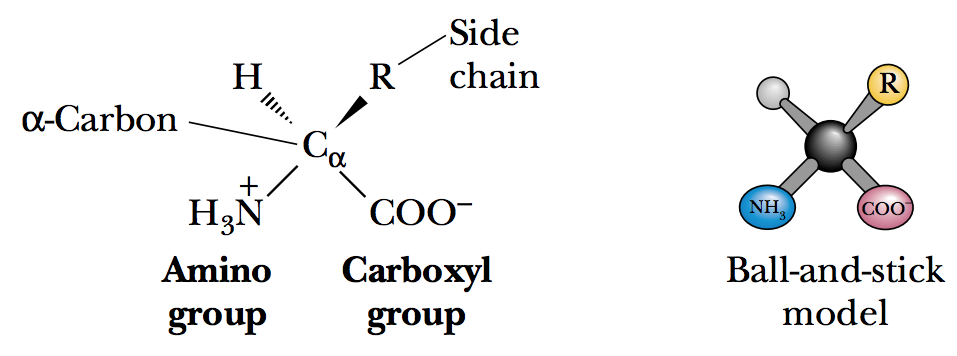
\includegraphics[width=0.7\textwidth]{Figuras/amino-acid.png}
    \caption{Amino Acid Structure (Source:~\cite{garrett1999biochemistry})}
    \label{fig:amino-acid-structure}
\end{figure}

Each amino acid has several designated identifications, as shown in
Table~\ref{tab:amino-acids}. The first column shows the amino acid name.
The second shows the 3 letter code. The third column shows the 1 letter code.
The 1 letter code is commonly used to describe amino acid sequences and
will be used throughout this work.

\begin{table}[h]
    \centering
    \begin{tabular}{c|c|c} \hline \hline
        Name          & 3 Letter Code & 1 Letter Code \\ \hline \hline
        Alanine       & Ala  & A \\
        Arginine      & Arg  & R \\
        Asparagine    & Asn  & N \\
        Aspartic acid & Asp  & D \\
        Cysteine      & Cys  & C \\
        Glutamic acid & Glu  & E \\
        Glutamine     & Gln  & Q \\
        Glycine       & Gly  & G \\
        Histidine     & His  & H \\
        Isoleucine    & Ile  & I \\
        Leucine       & Leu  & L \\
        Lysine        & Lys  & K \\
        Methionine    & Met  & M \\
        Phenylalanine & Phe  & F \\
        Proline       & Pro  & P \\
        Serine        & Ser  & S \\
        Threonine     & Thr  & T \\
        Tryptophan    & Trp  & W \\
        Tyrosine      & Tyr  & Y \\
        Valine        & Val  & V \\ \hline \hline
    \end{tabular}
    \caption{The 20 Naturally Occurring Amino Acids}
    \label{tab:amino-acids}
\end{table}

Each amino acid can be split into groups accordingly to its properties.
There are six commonly used groups~\cite{garrett1999biochemistry}:
The Aliphatic Hydrophobic; The Aromatic Hydrophobics; The neutrals;
The Basics (Positively Charged); The Acids (Negatively Charged);
and the Unique Amino Acids. The Aliphatic Hydrophobic group is composed of
Alanine, Isoleucine, Leucine, Methionine and Valine. The Aromatic Hydrophobic
is composed of Phenylalanine, Tryptophan and Tyrosine. The neutral group is made
out of Asparagine, Cysteine, Glutamine, Serine and Threonin. The acid group is
composed of the Aspartic acid and Glutamic acid. The basic group contains Arginine,
Histidine and Lysine. The Unique Amino Acids group contains Proline and Glycine.
The Knowledge of these groups allow for further insight into the amino acids
function inside a protein and are of valuable use in this work.

% Peptide bonds
The composition of two or more amino acids to compose a protein is called
a peptide bond. This bound happens between the amino group of an amino acid
and the carboxyl group of another amino acid. In this process, as shown in
Figure~\ref{fig:peptide-bond}, the carboxyl group loses an Oxygen and a Hydrogen
atom which bounds with an Hydrogen atom of the amino group from the other amino
acid. The bound is then formed between the carbon of the carboxyl group and the
nitrogen of the amino group. This process can happen several times, where each
time it happens a new amino acid is aggregated to the chain and a water
molecule is created in the process as a residue~\cite{garrett1999biochemistry}.

\begin{figure}
    \centering
    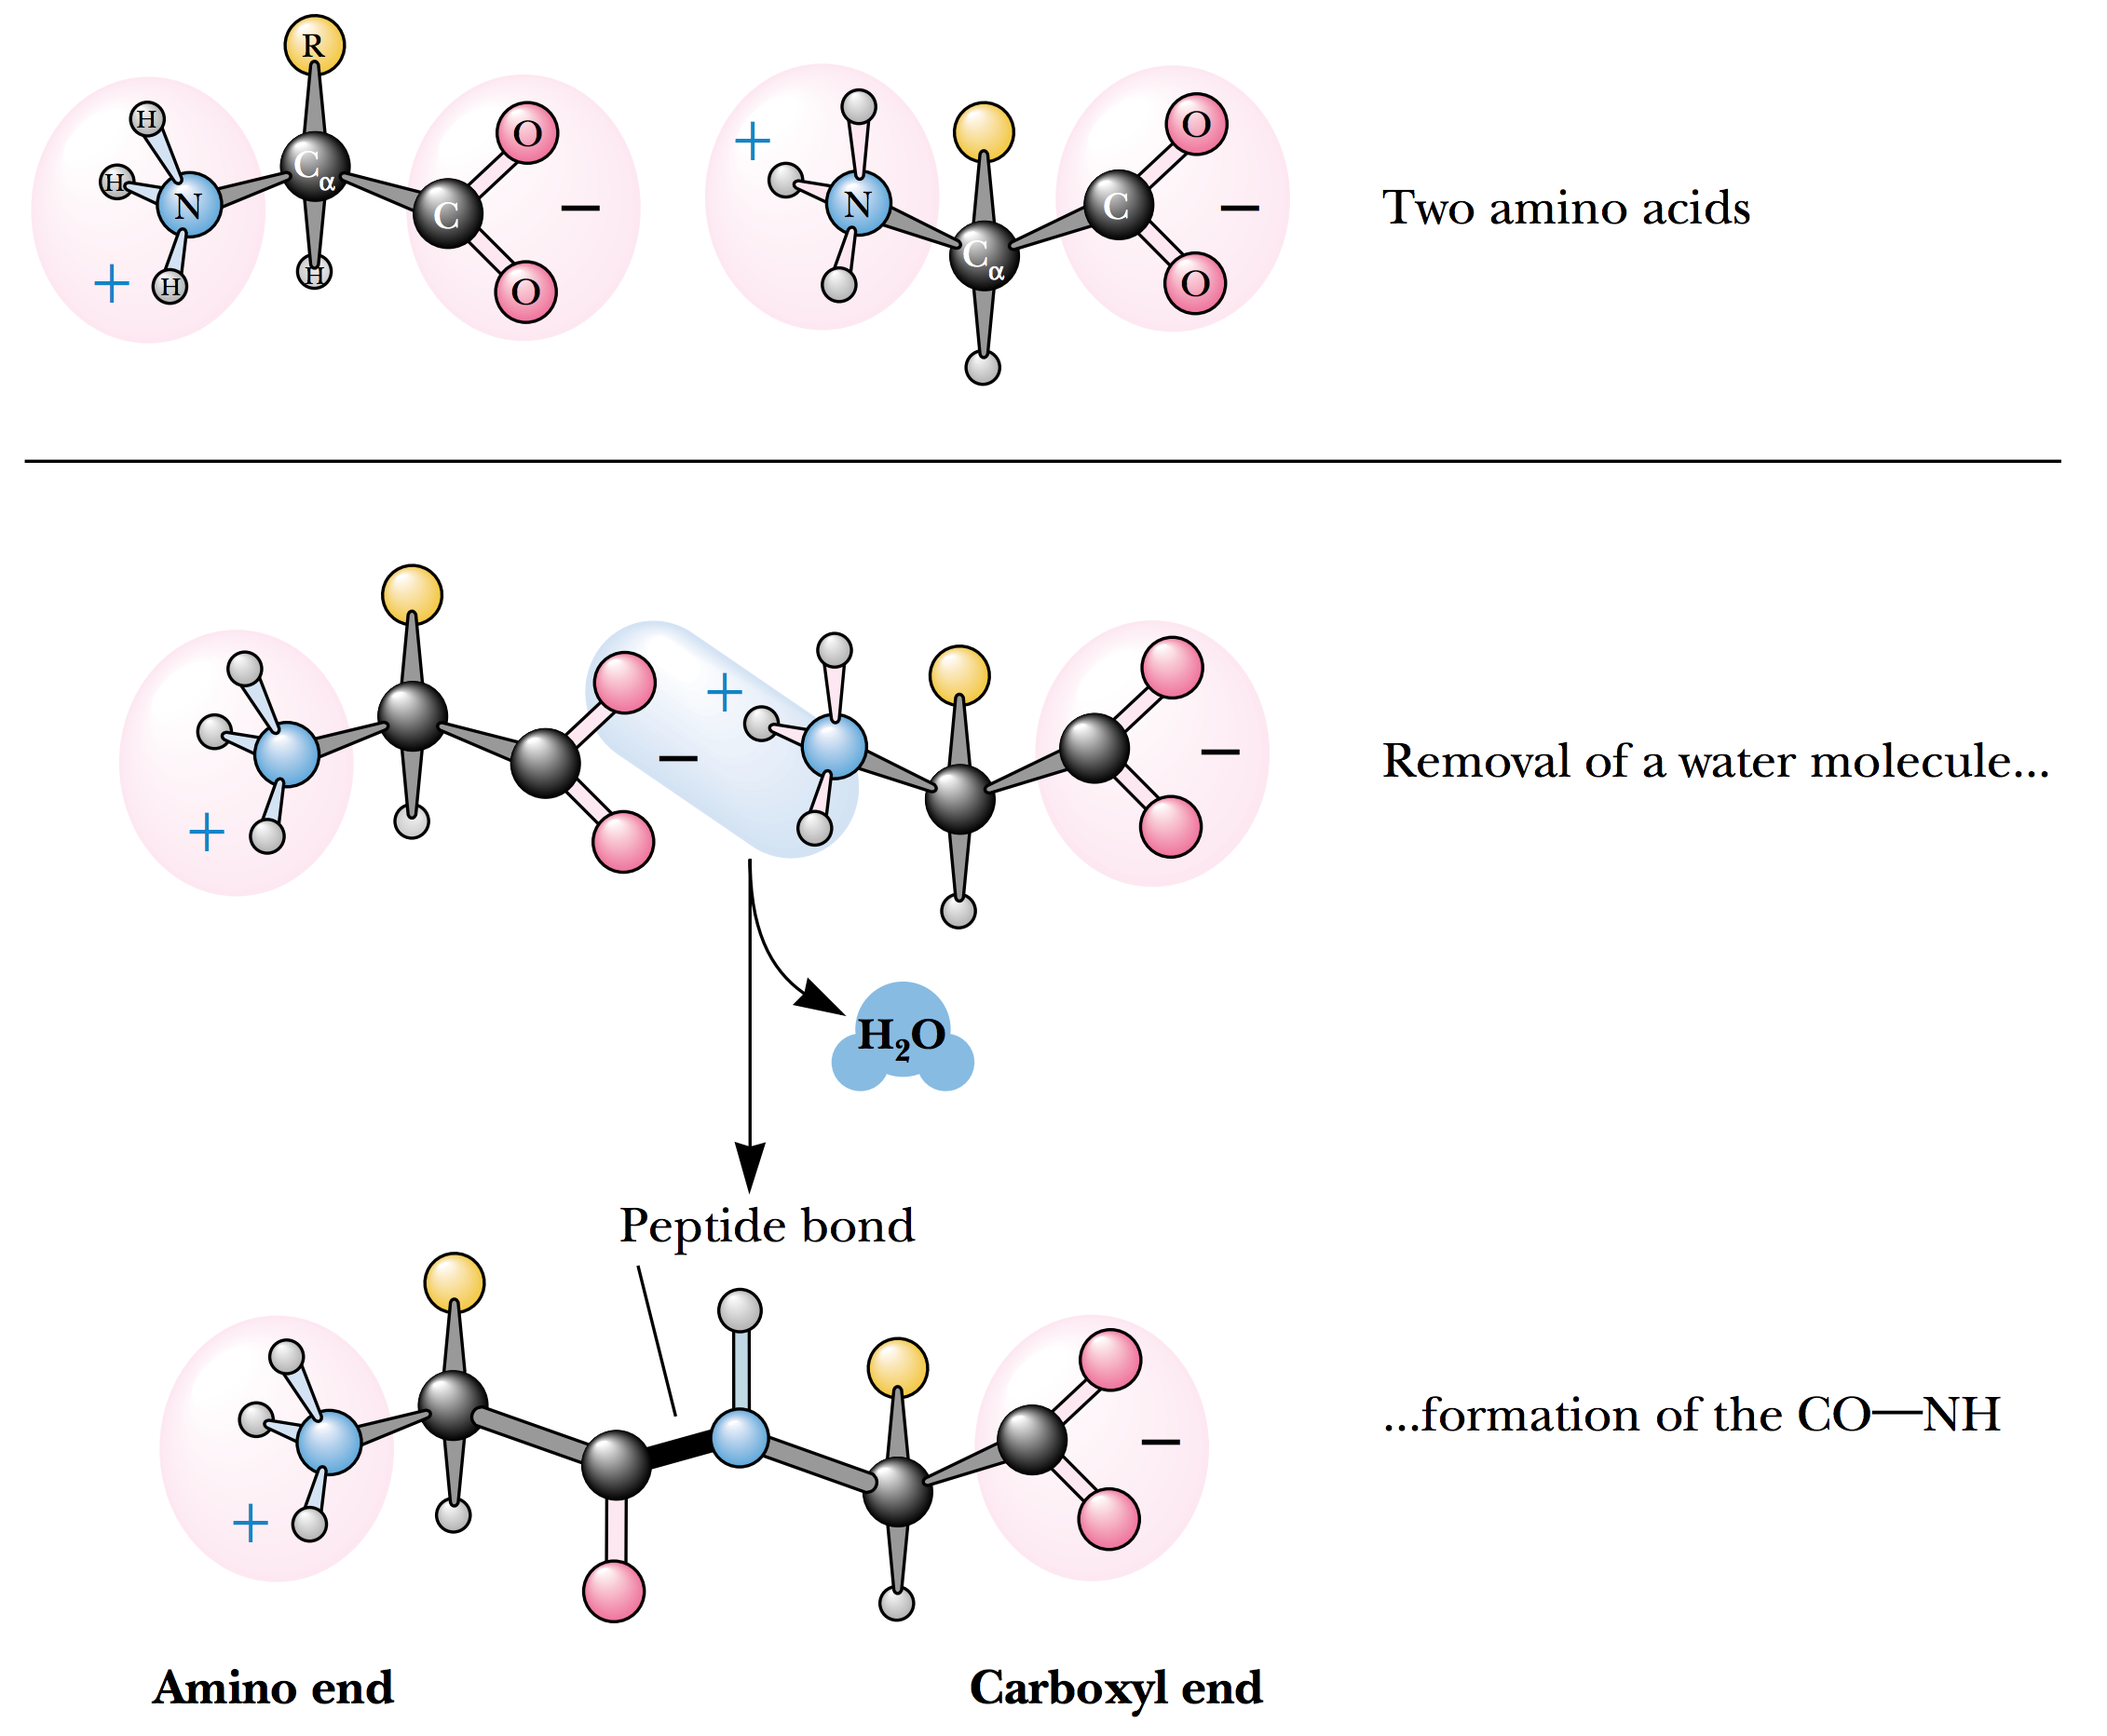
\includegraphics[width=\textwidth]{Figuras/peptide-bond.png}
    \caption{The Peptide Bond (Source: ~\cite{garrett1999biochemistry})}
    \label{fig:peptide-bond}
\end{figure}

When a peptide bond is formed and it starts to grow, it will assume a three
dimensional conformation. The manner in which the chain grows is directly
dependent on the dihedral angles that the peptide bond assumed. The dihedral
angles are enough to describe the protein to a high level of detail. The $N -
C_\alpha$ bound is described by the angle $\phi$. The $C_\alpha - C$ bound is
described by the angle $\psi$. Both the angles and $\phi$ and $\psi$ are
virtually free to rotate around its axis, limited only by steric clashes when a
part of the chain gets too close to itself. The $C - N$ pair is described by
the angle $\omega$. Due to complex interactions between the atoms in the chain
and its resonating properties, the $C - N$ bound behaves as if it was a double
bound. This limits the potential angles that $\omega$ can assume to regions
close to $0^{\circ}$ and $180^{\circ}$. The position where each dihedral angle
operates is shown on
Figure~\ref{fig:angles}.

\begin{figure}
    \centering
    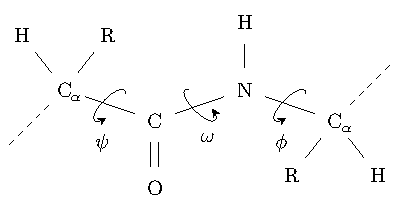
\includegraphics[width=0.7\linewidth]{Figuras/angles.pdf}
    \caption{Dihedral angles of an amino acid}
    \label{fig:angles}
\end{figure}

The sequence of bonds $N - C_\alpha$, $C_\alpha - C$ and $C - N$ is called the
backbone. This chain extends over all the protein and is responsible for the
shape that it assumes, along with its interactions with the side chains. Due to
the constraints for $\omega$, the $N, C_\alpha, H$ and $O$ atoms will tend to
be co-planar. Two possible configurations are possible, the \textit{cis} and
\textit{trans}. In the \textit{cis} configuration the $\omega$ angle will be
approximately $180^\circ$ and the side chains will have alternate sides after
each peptide bond. This configuration is the most stable one. For the
\textit{trans} configuration, which a $\omega$ angle of $0^\circ$, the side
chains will be on the same side, making this configuration much less stable and
consequently less frequent.

While the tuple $(\phi, \psi, \omega)$ of dihedral angles is enough to
accurately describe the backbone, it lacks information about the side chains.
Due to the nature of the side chains, different side chains will have different
dihedral angles. Table~\ref{tab:side-chain-angles} shows the amino acids and
the number of side chain angles required to describe it.

\begin{table}[]
    \centering
    \begin{tabular}{l|l} \hline \hline
        Amino Acid & Angles \\ \hline \hline
        GLY, ALA, PRO & N/A \\
        SER, CYS, THR, VAL & $\chi_1$ \\
        ILE, LEU, ASP, ASN, PHE, TYR, TRP & $\chi_1$, $\chi_2$ \\
        MET, GLU, GLN & $\chi_1$, $\chi_2$, $\chi_3$ \\
        LYS, ARG & $\chi_1$, $\chi_2$, $\chi_3$, $\chi_4$ \\
        \hline \hline
    \end{tabular}
    \caption{Side Chain Angles}
    \label{tab:side-chain-angles}
\end{table}

\subsection{Protein Structures}
\label{sec:protein-structures}
%What are primary, secondary, tertiary and quaternary structures

% Present the different levels of details of the proteins at micro and macro
% levels
The analysis of a protein happens on increasing levels of details. There are
four structures commonly used in proteomics to identify, study and describe a
given protein and its properties~\cite{tsai2003introduction}.

% Primary structure
The primary structure of a protein is determined by the chain of amino acids
that form it. This sequence is encoded on the \ac{DNA}, and after the protein
syntheses is complete it will be inside the protein. The primary structure is
unique for each protein and can be used to uniquely identify it. For instance,
the
\textit{Methionine-Enkephalin}\footnote{\url{https://www.rcsb.org/structure/1plw}}
(1PLW) is a very simple polypeptide formed by 5 amino acids: Tyrosine, Glycine,
Glycine, Phenylalanine and Methionine. Using the one letter notation, the
primary sequence can be presented as YGGFM. This one letter sequence of amino
acids is available on protein sequence databases, such as the UniProtKB
database\footnote{\url{https://www.uniprot.org/help/uniprotkb}}.

% Secondary
The secondary protein structure consists of local patterns occurring on the
protein conformation. These patterns are three dimensional and together they
are used to assemble the protein. There are 8 accepted protein secondary
structures: 3 types of helices, 2 types of sheets, turns, loops and
coils~\cite{geourjon1995sopma}.

% helices
The helices can be split into three types: $\alpha$-helix, $3_{10}$-helix and
$\pi$-helix. Helices are characterized for having the $i$-th amino acid bonded
to the $i+k$-th amino acid, for a sequence of several amino acids. This bond is
a hydrogen bond between the amino group of the $i$-th amino acid and the
carboxyl group of the $i+k$ amino acid. The values of $k$ vary from 3 to 5, and
they determine the type of helix.

The more common type of helix is the $\alpha$-helix, which has $k=4$. That is,
the amino group of an amino acid is bonded with a hydrogen bond to the carboxyl
group of the amino acid four positions (in the primary sequence) after. There
are approximately $3.6$ amino acids per $\alpha$-helix turn, as shown in
Figure~\ref{fig:alpha-helix}. The secondary chain of the amino acids in this
type of helix are located on the outside of the  helix. The amino acids inside
this type of helix will have torsion angles close to ($\phi$, $\psi$) = (-58,
-47). An $\alpha$-helix can have from only one turn (formed by 4 amino acids)
to more than thirty, such as the human keratin (4ZRY).

\begin{figure}
    \centering
    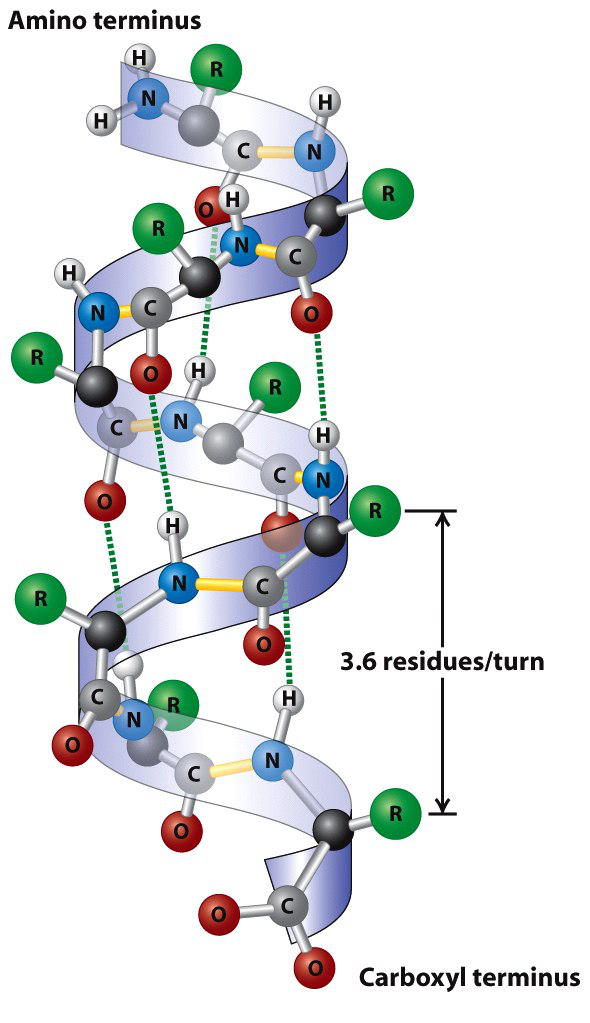
\includegraphics[width=0.5\textwidth]{Figuras/alpha-helix.jpeg}
    \caption{An $\alpha$-helix (Source:~\cite{lodish2008molecular})}
    \label{fig:alpha-helix}
\end{figure}

A seldom found type of helix is the $3_{10}$-helix. For this type of helix the
amino acids are bonded to the amino acid three positions after. This implies in
a helix more densely packed, and thus, less stable. Each turn has $3$ amino
acids and the torsion angles are around (-74, -4). A rarer type of helix is the
$\pi$-helix, where the hydrogen bonds happens 5 amino acids apart. There, each
turn as approximately 4.6 amino acids and the torsion angles are (-57, -70).
Accordingly to~\cite{borguesan2015apl}, $\alpha$-helix happens 34.1\% of the
time, $3_{10}$-helix less than 1\% of the time and $\pi$-helix about 4\% of the
time. Together, the three types of helix makes up for 39.1\% of the secondary
structures.

% Sheets
Another group of secondary structures are the sheets. They are characterized
for mainly for having planar surfaces. There are two types of sheets:
$\beta$-strands and $\beta$-sheets. The $\beta$-strands are sequence of usually
$3$ to $10$ amino acids with torsion angles of (-135, 135). $\beta$-strands and
$\beta$-sheets compose 25.2\% and 1.3\% of the secondary structures.

The $\beta$-sheets are formed from 2 or more $\beta$-strands, where each strand
bonds the adjacent ones. This bond is a hydrogen bond between the amino and
carboxyl groups of the amino acids, which happens in a alternating manner.
There are 2 types of $\beta$-sheets: Parallel and Anti Parallel. In the
parallel $\beta$-sheets all chains run in the same direction, as seem in
Figure~\ref{fig:parallel-beta-sheet}. In the anti parallel $\beta$-sheet the
chains runs in oposite directions, as represented in
Figure~\ref{fig:anti-parallel-beta-sheet}.

\begin{figure}[htbp]
    \centering
    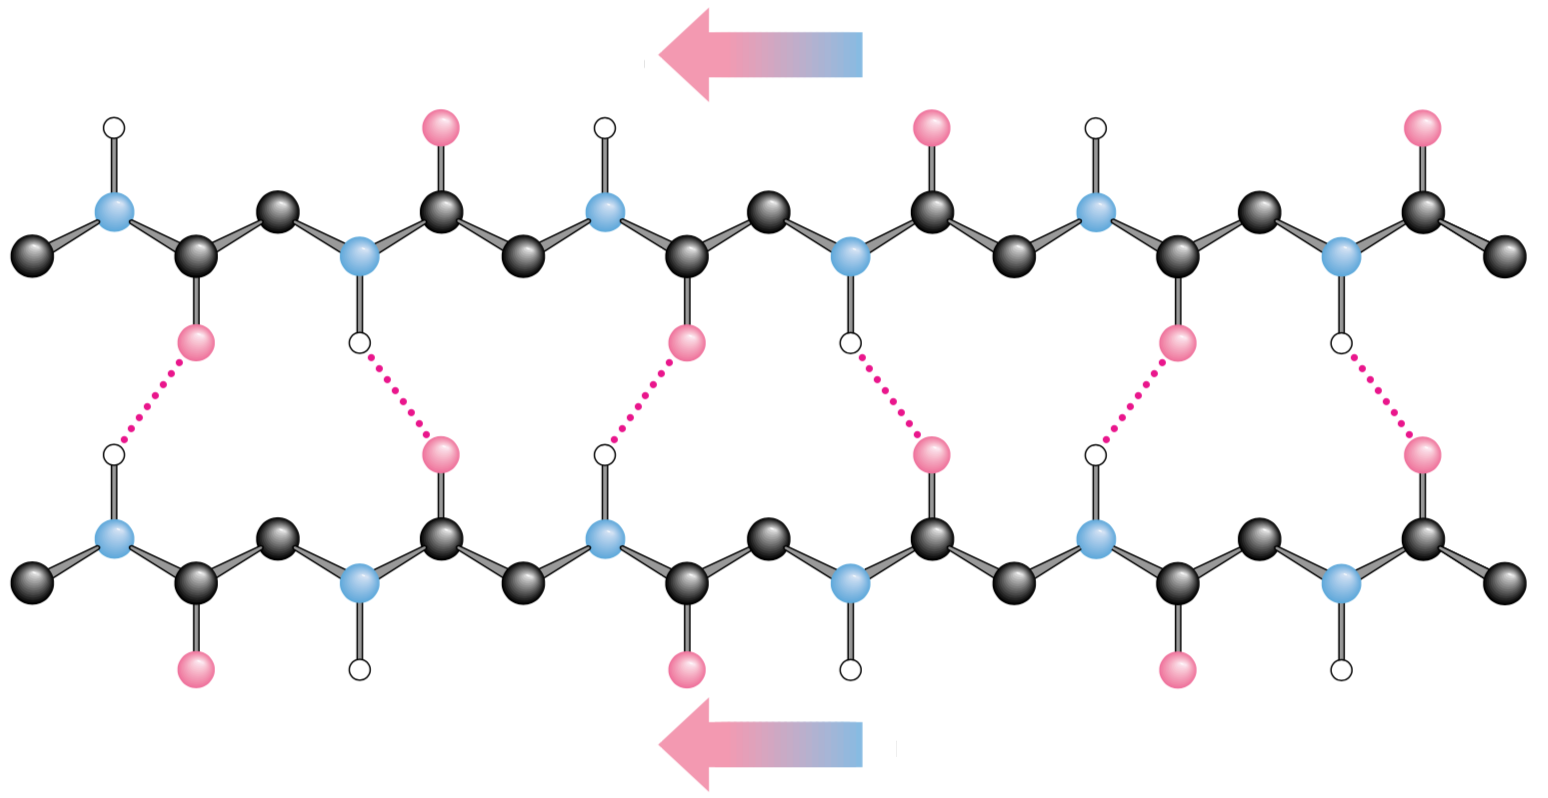
\includegraphics[width=0.5\textwidth]{Figuras/parallel-beta-sheet.png}
    \caption{A parallel $\beta$-sheet (Source: ~\cite{garrett1999biochemistry})}
    \label{fig:parallel-beta-sheet}
\end{figure}

\begin{figure}[htbp]
    \centering
    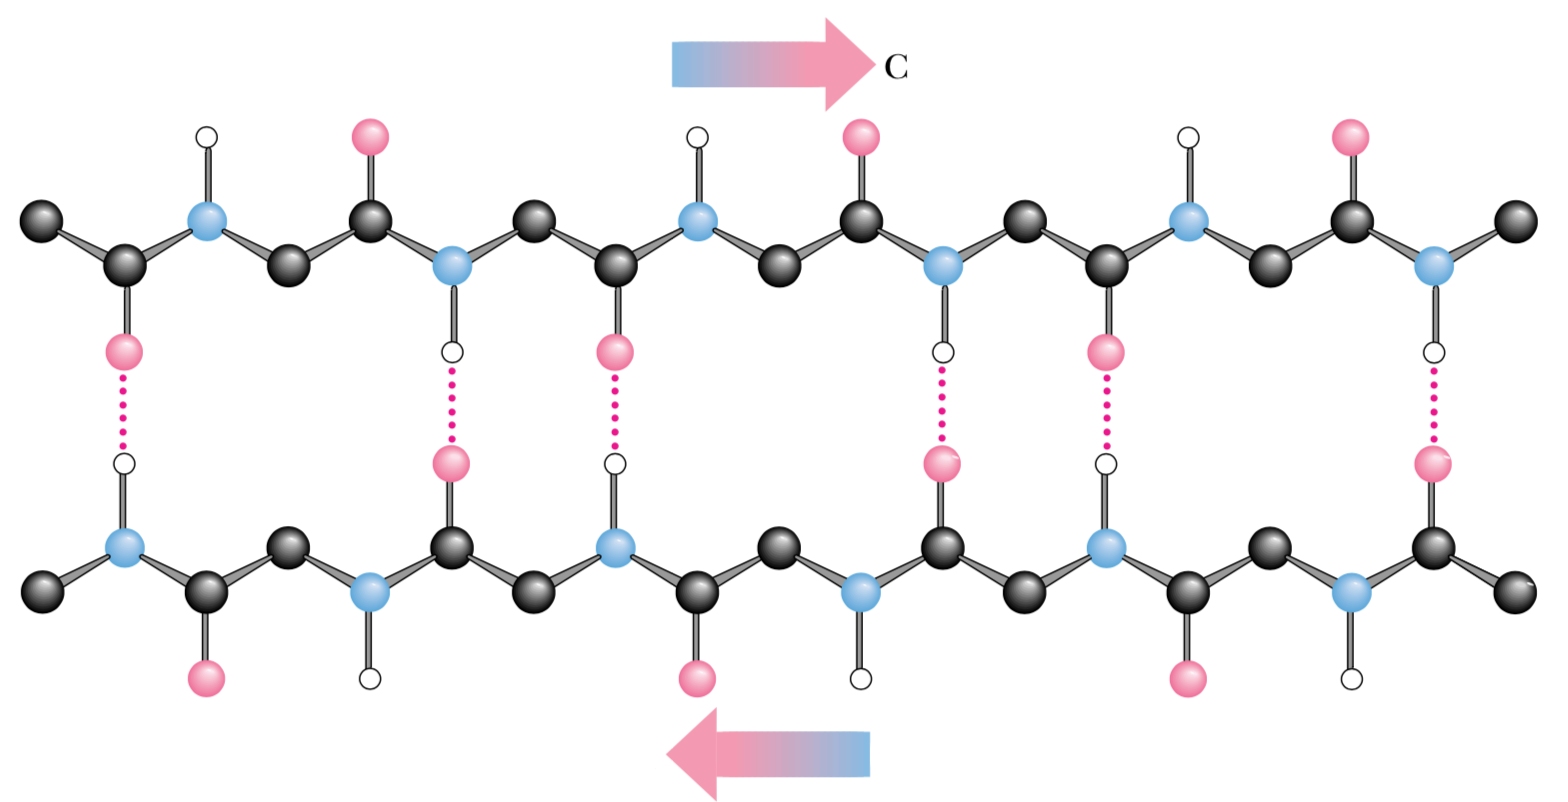
\includegraphics[width=0.5\textwidth]{Figuras/anti-parallel-beta-sheet.png}
    \caption{An anti-parallel $\beta$-sheet (Source: ~\cite{garrett1999biochemistry})}
    \label{fig:anti-parallel-beta-sheet}
\end{figure}

It is also possible for more than two $\beta$-strands to align forming a bigger
structure, called pleated sheets. In this structures, several $\beta$-strands
of the same alignment (parallel/anti-parallel) run along each other. This
allows for a $\beta$-strand to connect with the two neighbor $\beta$-strands.
An example of a anti-parallel pleated sheet in shown in
Figure~\ref{fig:pleated-sheet}. It is also possible that the ends of the sheet
bond to each other while being off-set by a single bond, thus making a shape
than resembles a cylinder.

\begin{figure}[htpb]
    \centering
    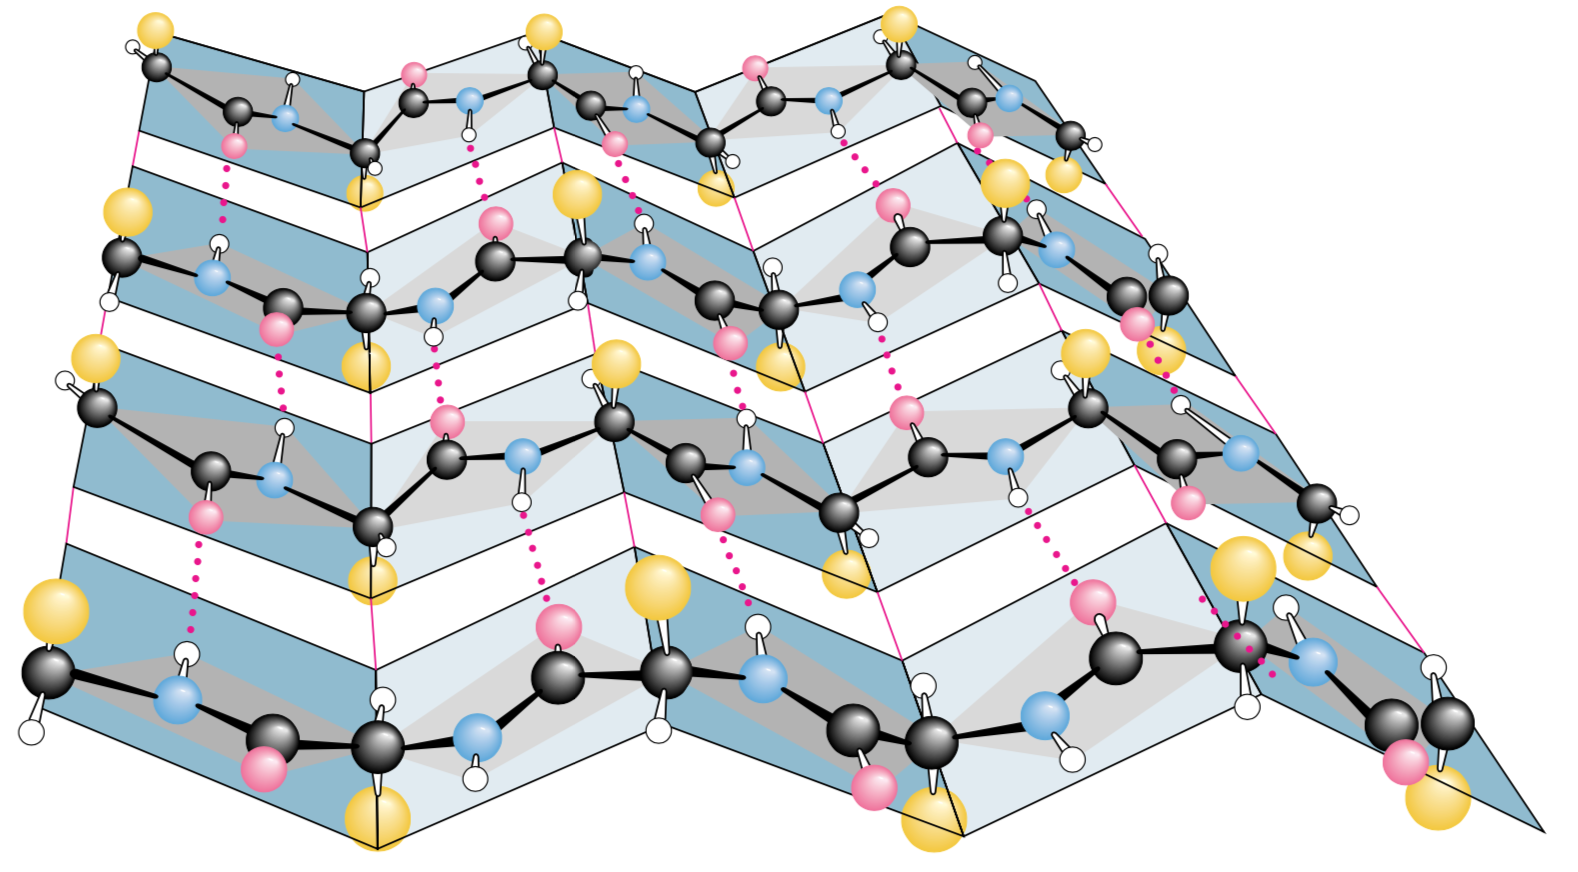
\includegraphics[width=0.75\textwidth]{Figuras/pleated-sheet.png}
    \caption{An anti-parallel pleated-sheet (Source: ~\cite{garrett1999biochemistry})}
    \label{fig:pleated-sheet}
\end{figure}

% other stuff (coils, turns and loops)
Finally, when there are no recurrent patterns on the secondary structure, it
can be either a loop, turn or a coil. A loop is a sequence of amino acids that
holds two helix or $\beta$-sheets together. If a loop is short and makes a
quick $180^\circ$ it is called a turn. If the amino acid sequence is located at
the start or the end of a protein, then it is called a coil. Turns and loops
represent 19.1\% of the secondary structures while coils represent 16.3\%.

% Tertiary
The tertiary structure is the three dimensional configuration of the amino
acids of a given protein. It can be also referenced as the native conformation.
The tertiary structure of a protein is directly dependant on the primary
structure. Also, the functionality of the protein is dependent on the tertiary
structure. A fact that rises the importance of being able to determine the
native conformation of a protein.

While the secondary structure references amino acids only locally, on the
tertiary structure all amino acids are relevant to the final structure.
Figure~\ref{fig:1ctf} shows a ribosomal protein of the Escherichia Coli
(1CTF)\footnote{http://www.rcsb.org/structure/1CTF} composed by 74 residues.
The figure shows the native conformation of the protein, i.e. its tertiary
structure. It also shows grouped in colors the secondary structures. The
$\alpha$-helices are presented in pink, $\beta$-sheets are presented in yellow
and white denotes coils. The combination of the secondary structures assemble
the tertiary structure. Furthermore, the tertiary structure describes how each
secondary structure relates to each other.

\begin{figure}[htbp]
    \centering
    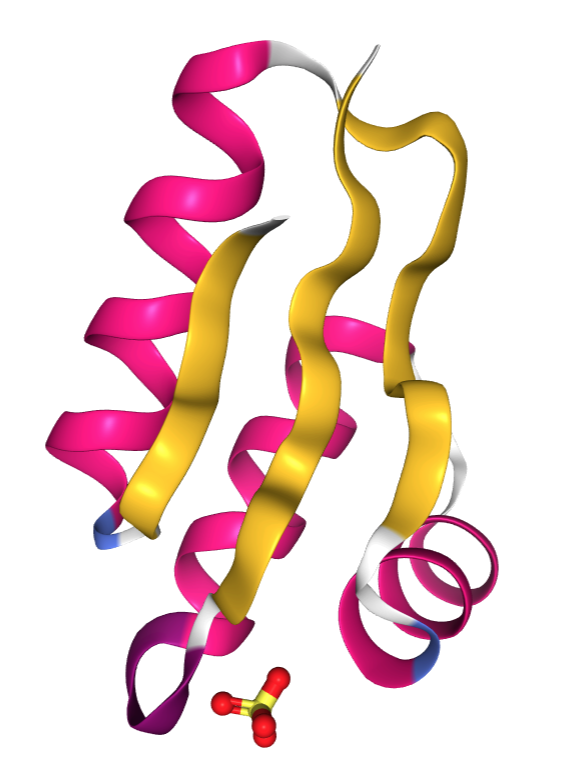
\includegraphics[angle=90,origin=c,width=0.6\textwidth]{Figuras/1ctf.png}
    \caption{The native conformation of protein 1CTF (Source: RCSB PDB)}
    \label{fig:1ctf}
\end{figure}

% Levintal's paradox describes a seemingly paradoxical situation where the protein

% Quaternary
There are certain groups of proteins that on its own are not able to exercise
its function. They need to be combined in pairs or even in bigger numbers. This
agglomeration of proteins is the quaternary structure, present in some (groups
of) proteins. A well know protein with a quaternary structure is the human
hemoglobin (1A3N)\footnote{\url{https://www.rcsb.org/structure/1a3n}}, formed
by 4 proteins. Figure~\ref{fig:human-hemoglobin} shows the assembly of four
proteins, the green point at the center shows a point of rotational symmetry
between the proteins.

\begin{figure}
    \centering
    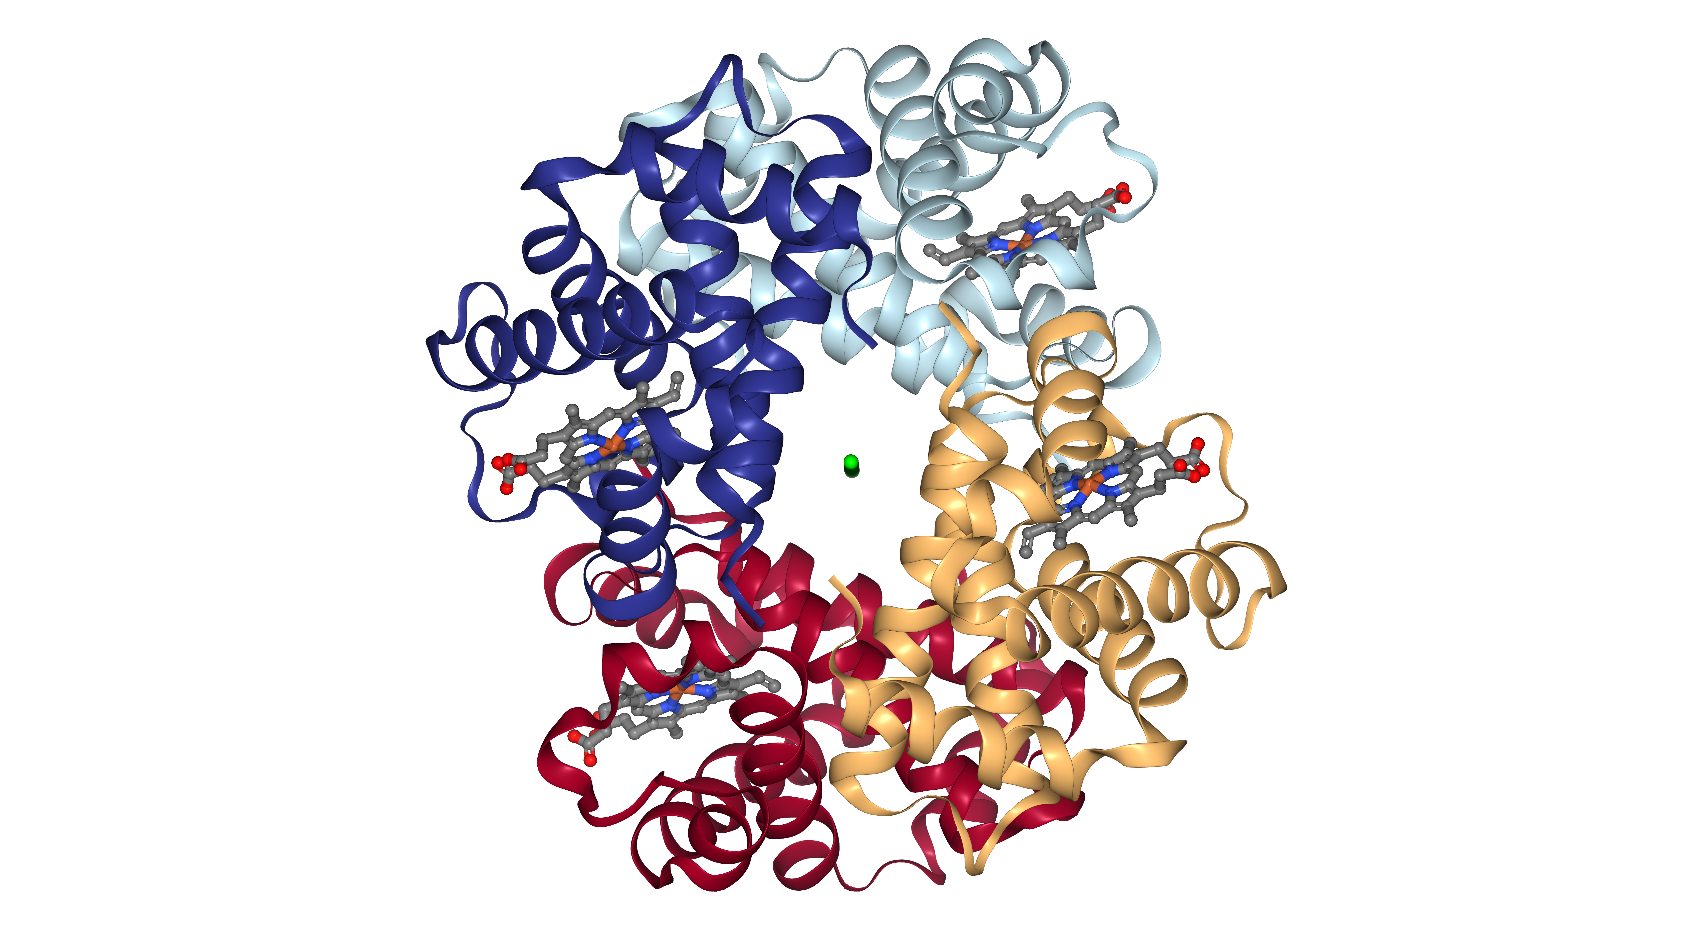
\includegraphics[width=0.6\textwidth]{Figuras/1a3n.png}
    \caption{The quaternary structure of the hemoglobin. Each color denotes one protein chain. The green point in the middle marks the point of radial symmetry. (Source: RCSB PDB)}
    \label{fig:human-hemoglobin}
\end{figure}

\subsection{Protein Secondary Structure Prediction}
\label{sec:secondary-structure-prediction}
%Secondary protein structure prediction problem

As previous shown on Section \ref{sec:protein-structures}, the secondary
structure plays a significant role in describing the native conformation of a
given protein. While not enough on its on, knowing in advance the secondary
structure of a protein allows one to work on how the groups of amino acids in
each substructure relates to each other instead of having to figure out how all
amino acids relates to each other. Therefore, knowing, even only approximately,
the secondary structure of a protein is a very important asset during the
process of predicting the tertiary structure.

Currently, there is no \textit{in vitro} method of determining only the
secondary structures of a protein. However, it is possible to employ
mathematical and computational methods. Considering that some amino acids have
more propensity of forming certain secondary structures, it is possible to
conduct an statistical analysis in order to assess the likelihood of an amino
acid forming a particular structure. This kind of analysis has been done
in~\cite{dunbrack1993backbone} and~\cite{borguesan2015apl}.

Given the number of proteins with a known structure, it is possible to use data
mining and artificial intelligence methods for predicting the secondary
structure. This approach is the more explored one so far.
In~\cite{wang2016protein} the authors used deep neural networks for predicting
the secondary structure. Feed forward neural networks were used
in~\cite{meng2016computational}. In~\cite{kathuria2018predicting} the authors
employed random forests to predict the secondary structure.
In~\cite{baldi1999exploiting} the authors used recurrent neural networks.
In~\cite{kim2018dihedral} the use of generative adversarial networks was
explored to predict the dihedral angles of the secondary structures.
In~\cite{pollastri2002improving} and~\cite{mcguffin2000psipred} the authors
used the output of (multiple) sequence alignment algorithms as the input of
simple feed forward neural networks. These two implementation were ranked top
in the \ac{CASP}~\cite{moult1999critical} and are still largely used to this
date. More details on secondary structure prediction are available
in~\cite{jiang2017protein}.


\section{Protein Structure Prediction}
\label{sec:psp}
\label{sec:pspp}
\label{sec:protein-structure}

%In contrast to the methods presented in Section~\ref{sec:protein-structure},
%\textit{in silico} methods required only information that is more easily and
%fastly obtainable. At this point, however, they are not viable for larger
%(more than 100 amino acids) proteins. Nevertheless, a significant effort has
%been put into improving the current methods.

%In this section it is presented topics on protein computational
%representation, on and off lattice models and the main prediction methods are
%presented as well.

%\subsection{Protein Representation} \label{sec:protein-representation} on and
%off lattice

In a laboratory environment, i.e. \textit{in vitro}, it is possible to
determine the native conformation of a given protein using mainly two methods.
The first method is know as X-Rays crystallography~\cite{nelson2008lehninger}.
Overall, the X-Ray crystallography has a better quality in the data generated,
however, it can only work on crystallized structures. Due to this fact, it is
possible that during the process of crystallization of a given protein sample
it crystallizes in a conformation that is not exactly its native one. Proteins
\textit{in natura} are dynamic molecules, that can vibrate and tumble around.
This property is lost when using X-Ray crystallography.

The other more recent method is ~\ac{NMR}~\cite{nelson2008lehninger}. This
method has a slighter lesser accuracy, however, it can work with proteins in an
aqueous environment. Thus, having a trade off that can offset the downsides of
X-Ray crystallography. Nevertheless, both methods are error prone, possibly
outputting noisy data. They also are expensive and take a considerable human
effort and economic resources to be utilized.  Thus the need for a \textit{in
silico} method of determining/predicting the protein structure.

The process of predicting the structure of a protein requires that it be
represented computationally in some way. The folding process \textit{in natura}
happens very fast, spontaneously and in a continuous environment. However, in
order to represent the protein computationally, some trade off is required
between level of detail and processing power required. Arguably the main
division between the models are the on lattice models and the off lattice
models.

The on lattice model, as the name implies, are models where the structures are
constrained to a lattice. Possibly the simplest model is the 2D \ac{HP} Model.
It is composed of points representing the amino acids, which can be either
hydrophobic or polar and are constrained to a 2D quadrilateral lattice. Despite
its simplicity, this model is already
$\mathcal{NP}$-complete~\cite{berger1998protein}. A 3D approach to a \ac{FCC}
lattice is presented in~\cite{hoque2007protein}, which also is a
$\mathcal{NP}$-complete problem. A triangular lattice approach is studied
in~\cite{agarwala1997local} in two and three dimensions. At the time of the
publication it was not know if that particular model was a
$\mathcal{NP}$-complete problem, latter it was proved to be. In fact, as
demonstrated by~\cite{hart1997robust}, the protein structure prediction problem
is $\mathcal{NP}$-complete regardless of the lattice used to represent it.

% explain off lattice models
Despite the on lattice model simplicity, it still is an intractable problem on
large scale due to its $\mathcal{NP}$-completeness. Furthermore, from a
practical point of view, these models can not represent a protein with enough
details to be able to replace an \textit{in vitro} method for determining the
protein structure. Therefore, a more robust representation is required. This
higher representation power is possible using off lattice models, that is, a
model that is not constrained by a lattice.

What can possible be considered the simplest model is the AB Off lattice model,
which represents the amino acids as spheres that are either hydrophobic or
polar, and the angles between them are not
constrained~\cite{berger1998protein}.  A more detailed model consists of using
the coordinates of the $C_\alpha$. In this model the amino acids are abstracted
into spheres, however, they maintain their properties such as polarity and
hydrophobicity, allowing for a increased level of detail. It is possible to
represent each of the amino acid heavy atoms (Nitrogen, Carbon and Oxygen)
individually, instead of using an sphere to represent the whole amino acid.
This model allows for interactions between individual atoms in the  backbone to
be considered during the prediction.

Evolving even more the level of detail, it is possible to represent all atoms
in the backbone, including the Hydrogen atoms. This permits that hydrogen bonds
be taken into account, which plays a significant role in the formation of
secondary structures and in the interactions between them. Furthermore, it is
possible to include an ellipsoid (also called centroid) to describe the amino
acid side chain. With this, the shape of each amino acid also can be considered
when predicting the three dimensional structure of the protein.

To fully represent the protein, there are two main models. Backbone and side
chain torsion angles and all atoms coordinates~\cite{rohl2004protein}.  The
former describes all atoms in the protein, including the side chain. However,
the bond length between these atoms are fixed as well as the position of the
hydrogen atoms. This model is enough to describe the protein very accurately
and to take into account most of its interactions. Nevertheless, since
artificial constrains are imposed in the model, it is possible that some
proteins can not be correctly predicted because it depends on one of the
aspects that the model removed. For this reason the all atom coordinates model
can be employed. In this model all atoms are considered and have all their
degrees of freedom. Currently, this model is the most accurate one, at the
expense of adding up a hundred variables per amino acid.

\subsection{Ab Initio Methods}\label{sec:ab-initio}

One of the main class of protein prediction algorithms are the ab initio
methods~\cite{lee2017ab}. From the Latin, ab initio means \textit{first
principles}. These methods are called as such because they work based only on a
primordial aspect of the proteins: They are physicochemical objects. And as
such, they follow well know rules.

The information about the physical and chemical properties from the proteins
are encoded on the protein representation as discussed on
Section~\ref{sec:pspp}. Its interactions are evaluated by energy functions (or
scoring functions). A given protein \textit{in natura} seeks its point of least
potential energy~\cite{anfinsen1973principles}. Based on this fact, an energy
function for an \textit{ab initio} method tries to evaluate the potential
energy of a given conformation. Then, with a search procedure it is
(theoretically) possible to find its point of least potential energy, which
should be at least close to its respective native conformation. In other words,
\textit{ab initio} methods can be seem as an optimization problem where the
objective function is the energy function of the protein and its variables are
the degrees of freedom from its computational representation.

% present some energy functions
There are several energy functions in the literature which allows for an
\textit{ab initio} approach, such as the \ac{AMBER}, \ac{GROMOS}, \ac{CHARMM} e
Rosetta.  The \ac{AMBER}~\cite{salomon2013overview} package contains a set of
scoring functions based only on the potential energy of proteins (and other
molecules). Its original use was intended for molecular dynamics simulations.
However, its is possible to use it just to score a given conformation. Another
package which offers energy functions for proteins is
\ac{CHARMM}~\cite{brooks2009charmm}. Similar to \ac{AMBER}, it is also
primarily intended for molecular dynamics simulations for several organic
molecules of interest. Nevertheless, its scoring can be used for \textit{ab
initio} methods. The \ac{GROMOS} package~\cite{eichenberger2011gromos++} also
intended for molecular dynamics simulations can provide energy scoring of
protein conformations. A more detailed discussion of the energy functions is
available at~\cite{dorn2014three}. In~\cite{narloch2016diversification}
explored the differences between \ac{AMBER}, \ac{CHARMM} and Rosetta. A further
discussion on energy fields (from molecular dynamic packages) can be found
in~\cite{vlachakis2014current}.

Several energy functions are used in the literature. The Rosetta
suite~\cite{rohl2004protein,kaufmann2010practically} contains multiple energy
functions for all atom coordinates models, backbone and side chain torsion
angles and backbone torsion angles with centroids for the side chains. This
suite also allows for the customization and creation of new energy functions.
The energy functions there consider both the physicochemical properties of the
protein as well as its statistical nature, based on a knowledge database with
propensities of each amino acids. Information regarding the compactness of the
structure and other properties such as the formation of side chain structures
are also computed. This removes the possibility of scoring the protein with an
physical unit of measurement. Instead, the energy functions are measured by the
\ac{REU}. More information about the information considered is available
in~\cite{alford2017rosetta}.

% Briefly present the optimizers
With an energy function for scoring the protein conformations, it is possible
to employ an optimizer in order to search for an conformation of least
potential energy. This procedure must sample the conformation space accessible
from the computational representation of a given protein. A vast range of
methods has been employed over the years in the literature.
In~\cite{li1987monte} a Monte Marlo based search is used to optimize a set of
dihedral angles. Basin-hopping is a method where a random perturbation is
applied to the conformation and then a hill-climbing type of algorithm is
employed to find a local minima. It has been used in~\cite{prentiss2008protein}
and~\cite{olson2012efficient}.

One particular branch of algorithms that have been used extensively in the
literature are bio inspired algorithms. The more well established algorithms
are present in the literature, such as the \ac{PSO}~\cite{geng2017protein},
\ac{DE}~\cite{hao2017conformational} and the \ac{GA}~\cite{higgs2010genetic}.
Other algorithms that are not so widely used have been also explored for the
\ac{PSPP} such as the Cucko Search (CS)~\cite{ramyachitra2017modcsa} and the
Bee Colony Algorithm~\cite{li2015balance}. This topic is explored in further
detail in Section~\ref{sec:bioinspired}.

\subsubsection{The Rosetta Suite} \label{sec:rosetta}

Practically, working with an \textit{ab initio} method is very time consuming,
due to the high amount of boilerplate code required to be able to model the
protein and its molecular dynamics from scratch. Furthermore, this process is
also very error prone. The Rosetta Suite~\cite{rohl2004protein} introduces a
robust and validated suite for working with proteins and other macromolecules.
It also includes multiple utilities for manipulating, pre-processing and
post-processing the protein conformations in a pipeline. The Rosetta Suite is
free for academic use, open-source and is available at
\url{https://www.rosettacommons.org/}.

One of the tools available at Rosetta and required for this work is fragment
insertion. A fragment consists of a sequence of continuous amino acids at a
specific configuration extracted from some protein of known structure. This
sequence must fully match to some continuous sequence of amino acids in the
target protein, where the structure is not yet known. The purpose of this is to
use multiple fragments as building blocks. It is worth noting that fragments
from homologous structures are removed, as for to remove the potential sampling
from the same protein from another organism for example.

The process of creating a set of fragments for a particular target protein
is required to be run only once per target and per fragment size. Two sizes of
fragments commonly used are 3 and 9. So if a fragment set is being created
for a given target protein, then the fragment picker must be run twice. The
fragment picker is the module responsible by searching a database of
non redundant protein conformations and sampling it in order to assemble
fragments. More information about the inner workings of the Rosetta Fragment
Picker is available at~\cite{gront2011generalized}.

Rosetta includes two fragment insertion operators (called \textit{movers} in
Rosetta). One is the classical\footnote{Found in Rosetta as
ClassicFragmentInsertion} fragment insertion and the other operator is the
smooth\footnote{Found in Rosetta as SmoothFragmentInsertion} fragment
insertion. The classical operator simply replaces one portion of the protein
with its respective fragment. This change can be very aggressive and have a
high changing impact on the protein conformation. Due to the high impact of
this operator, there is a high chance that the operator will produce a
conformation with a worse energy score, and therefore be rejected if used under
a \ac{MC} search.

The smooth fragment insertion applies a classic fragment insertion followed by
a second fragment insertion that tries to minimize the Gunn
Cost~\cite{gunn1997sampling}. The Gunn Cost measures the amount of change in a
conformation due to the arm lever effect. That is, the further away from the
insertion point an amino acid is, the more it will move. Since the smooth
fragment insertion tends to negate some of the change it will preserve some of
the structure of the protein, leading to a more localized change in the
conformation. It is worth noting that the smooth fragment insertion is an
optimization problem as well, which minimizes the Gunn Cost.  Since this
operator tries to minimize the amount of change by its application, the impact
on the energy score will be smaller, leading to smaller and more refined
changes. This, under a \ac{MC} situation will potentially lead to a higher
acceptance rate.

\subsection{Knowledge Based Methods}

% Why use it
Due to the limitation that \textit{ab initio} methods currently have, other
methods have been utilized in the literature with greater success. These two
methods are the \ac{TM} Methods~\cite{dorn2014three} and \ac{HM}
Methods~\cite{leach2001molecular}. Contrary to the \textit{ab initio} methods,
these two methods require previous information to be available in order to be
successful.

%Threading
\ac{TM} assumes that protein structure is, to some degree, preserved during the
evolution of organisms. Therefore, proteins with a certain degree of difference
in the primary sequence may have a very similar tertiary structure. A set of
template proteins is used as to represent the conformation space. Then, the
amino acid sequence of the target and template protein are aligned in order to
fit the target protein into the template. Then, the model is refined and the
final prediction is then output. In the event of the target protein having the
same overall fold as the template, the prediction can achieve very high levels
of accuracy. However, if a suitable template can not be found, the prediction
will be of poor quality. This is one of the main downsides of the \ac{TM}
method. It requires a suitable template. Nevertheless, \ac{TM} has had the best
results in recent \ac{CASP} events~\cite{moult2018critical}.

%Homology
\ac{HM} is to an extent similar to \ac{TM}. However, while \ac{TM} relies on
potential evolutionary similarities between proteins, HM expects homologous
(similar primary sequence) to have similar tertiary structures. Thus, HM
depends on the existence of a protein with a sufficient degree of similarity.
If such protein exists (and has its native conformation available) then it is
possible to arrive a high degrees of accuracy.

% downsides
Both \ac{TM} HM require that a suitable known protein to exist to be used as
template. Either one with evolutionary similarity for \ac{TM} a homologous
protein for HM. If such proteins do exist, then these methods will have a very
high chance of outperforming \textit{ab initio} methods. However, as the degree
of similarity decays so does the performance of the method. At this point
\textit{ab initio} methods have a chance of outperforming knowledge based
methods.

\subsection{Evaluating Protein Errors}\label{sec:protein-metrics}

Regardless of the method being used for predicting the protein structure, in
order to conduct research in this area it is necessary to measure error in the
prediction. Error measurement has been an active sub area of research in the
\ac{PSP} field, with dozen of such metrics being proposed since the \ac{PSP}
started to grow in
interest~\cite{xu2010significant,zhang2005tm,siew2000maxsub}.  Different
metrics focus on different aspects of the prediction, and while they should be
somewhat directly correlated between then it is possible that different metrics
do not always agree on the quality of a prediction. Therefore, it is important
to know the metrics and how they can evaluate a prediction.

Currently, when conducting a research, the main way of measuring error is to
compare the predicted structure against the one that was found \textit{in
vitro}. With this, it is possible to measure how far (or close) a prediction is
from the ground truth. This approach, however, has some flaws. The main one is
that determining the protein structure \textit{in vitro} has an error margin.
That is, the native conformation found by \ac{NMR} and X-Rays crystallography
methods has a finite resolution, typically in the order
of 1 to 3 Angstroms. Due to that, getting and error too low is rather
pointless, since instead of measuring against the native conformation
it would be measuring against the method itself. Other point that is
worthwhile to take into account is that it may be required to have the
protein in a crystal form in order to study its conformation
\textit{in vitro}. Naturally, the proteins are in an aqueous environment,
surrounded by several substances. The crystallization process therefore
removes the protein from its natural environment and forces it in a
solid state~\cite{wuthrich1989protein}.
This also inserts some degree of error into the model. As it can be seen
on Figure~\ref{fig:protein-error}, 19 conformation samples obtained
\textit{in vitro} are superimposed and show a noticeable variation.
This variation occurs dues to the reasons listed above.

\begin{figure}
    \centering
    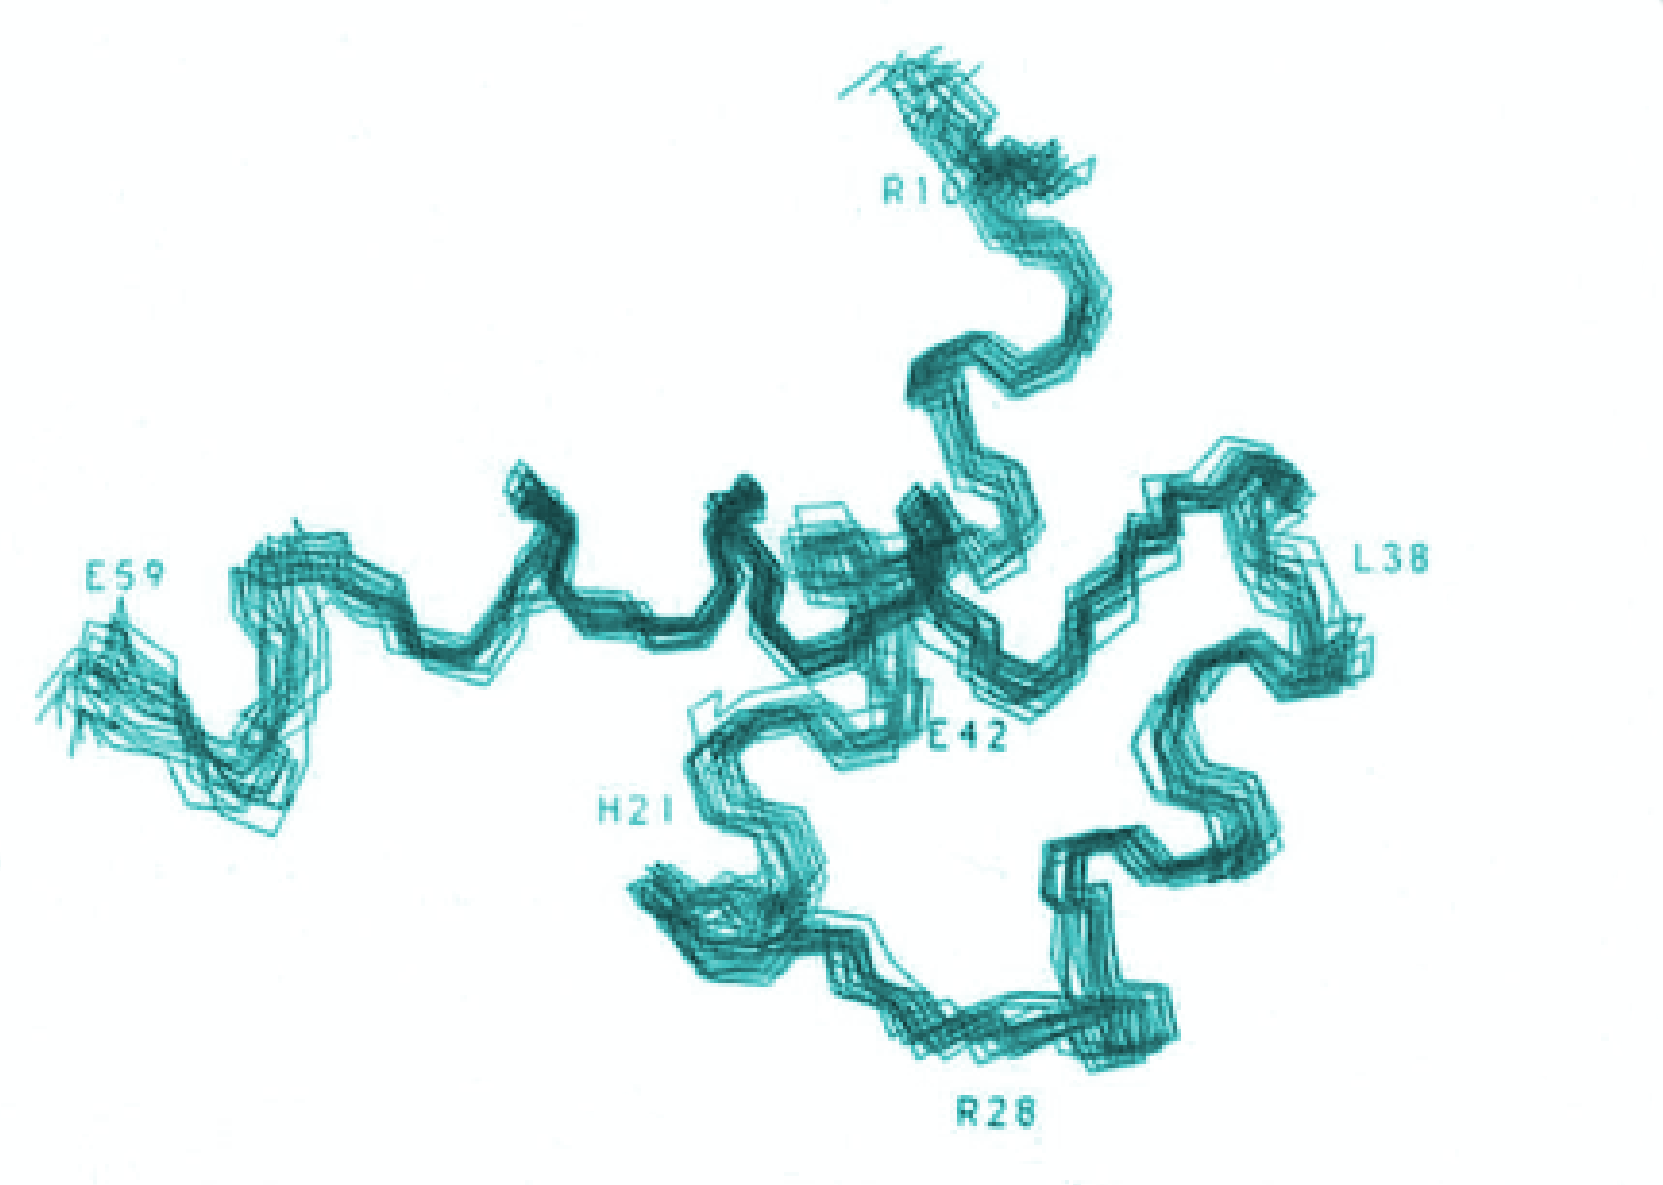
\includegraphics[width=0.7\linewidth]{Figuras/protein-error.png}
    \caption{19 aligned samples of a protein determined by \ac{NMR} (SOURCE (ADAPTED): \cite{wuthrich1989protein})}
    \label{fig:protein-error}
\end{figure}

Possibly the most well known protein prediction measuring method is the
\ac{RMSD}. It is typically applied to the alpha carbons, and thus only
measuring the error in the backbone. However, it can also be applied to all
atoms in the protein. The formula for the \ac{RMSD} is shown in
Equation~\eqref{eq:rmsd}. As the name suggests, the \ac{RMSD} is calculated as
the Square Root of the mean from the squared deviation.

%\textbf{REVEJA ESTAS EQUAÇÕES, PRINCIPALMENTE ONDE APARECEM RAIZ QUADRADA E
%DIVISÕES.} \textcolor{red}{O q exatamente é pra rever?}

\begin{equation} RMSD (A, B) = \sqrt[2]{\frac{\sum^{n}_{i = 1}{(A_i -
B_i)^2}}{n}} \label{eq:rmsd} \end{equation}

The fact that the deviation is squared and averaged leads to some downsides in
this measurement method. Firstly, a bigger protein can have a much higher error
due to the deviations being squared over the number of atoms being considered.
This makes the comparison of prediction quality between different proteins
impractical. For example, an error of $4{\AA}$ in a 50 residue protein is
different from $4{\AA}$ in a 150 residue protein. Furthermore, since the
deviation is squared, small deviations in some keys places of the conformation
will lead to an error that propagates over the protein due to an arm lever
effect.

In order to avoid the downsides of the \ac{RMSD}, several other metrics have
been proposed. Two of them saw great use in \ac{CASP}~\cite{moult2018critical}:
\ac{GDT-TS}~\cite{zemla2003lga} and the \ac{TM-Score}~\cite{zhang2004scoring}.
\ac{GDT-TS}, meaning Global Distance Test-Total Score is a measurement which
considers four successive alignments and is shown in Equation \ref{eq:gdt-ts}.
Each alignment uses a cutoff from $1{\AA}$ to $8{\AA}$ going in powers of two.
The score consists of the mean of the ration of the maximum number of atoms
that can be aligned using there cutoffs. It is worth noting that calculating
the \ac{GDT-TS} is a $\mathcal{NP}$-Hard problem on its own. Nevertheless,
heuristics that are sufficiently fast and accurate have been developed to make
it of practical use.

\begin{equation} \text{GDT-TS} = ( GDT_1 + GDT_2 + GDT_4 + GDT_8 ) / 4
\label{eq:gdt-ts} \end{equation}

The \ac{TM-Score} can be considered an extension of the \ac{GDT-TS}. While
\ac{GDT-TS} improves upon \ac{RMSD}, it has some downsides of its own. For
instance, the fixed thresholds may lead to semantic differences when
considering proteins of different sizes. That is, a smaller protein will be
able to fit more atoms inside the threshold more easily than a bigger protein,
thus rendering the measurement method somewhat dependent on residue length,
even though the score is normalized between 0 and 1.

\ac{TM-Score} aims to provide a dynamic threshold value based on the protein
length, and with this, provide a more meaningful score regardless of the
protein length. \ac{TM-Score} also allows for proteins of different size to be
compared. It is worth nothing that the \ac{TM-Score} of A compared to B is
different from B compared to A (unless they have the same size).
Equation~\eqref{eq:tm-score} shows how the error is measured, where
$L_{target}$ is the length of the target protein (the native conformation in
the case of the \ac{PSP}) and $L_{aligned}$ is the protein which is being
evaluated (the predicted conformation in the \ac{PSP}). The distance between
two pair of atoms $i$ is $d_i$. The dynamic threshold is shown as $d_0$ in
Equation~\eqref{eq:tm-score-d0}.


\begin{align}
    \text{TM-score}&=\max\left[ \frac{1}{L_\text{target}}\sum_i^{L_\text{aligned}}\frac{1}{1+\left(\frac{d_i}{d_0(L_\text{target})}\right)^2} \right] \label{eq:tm-score} \\
    d_0(L_\text{target})&=1.24\sqrt[3]{L_\text{target}-15}-1.8 \label{eq:tm-score-d0}
\end{align}

When comparing \ac{GDT-TS} and \ac{TM-Score} to \ac{RMSD} some key points are
worth noting. Firstly, \ac{RMSD} scales quadratically, meaning that the same
difference between the \ac{RMSD} of two conformations at difference magnitudes
are not necessarily equally proportional. For example, the error between two
conformations of an \ac{RMSD} of 2 and 3 is bigger than two conformations of
\ac{RMSD} 6 and 7. \ac{GDT-TS} offers a linearly proportional metric. Another
key point is that \ac{GDT-TS} and \ac{TM-Score} offers a normalized value which
is meaningful over different proteins. That is, it is possible to measure if a
method performs better on one protein on another directly. Lastly, studies such
as~\cite{xu2010significant} shows that some values of these scores can be used
as milestones. For instance a value of 0.5 or higher indicates that the same
fold was achieved. For \ac{GDT-TS} a score less than 0.2 corresponds to the
performance of a random search. For \ac{TM-Score} that value is somewhere
between 0.15 and 0.2. With this information it is possible to evaluate a
methods performance using only these error metrics.

% \section{Bio Inspired Metaheuristics}~\label{sec:bioinspired}
\section{Optimization}~\label{sec:bioinspired}

% Present and show its applications
As shown in Section~\ref{sec:ab-initio}, \textit{ab initio} methods require an
objective function and an optimizer for it in order to search for a
conformation of low potential energy where its performance depends both on an
accurate energy function and a robust search procedure for optimization.
Several search methods can be utilized for this purpose. However, it is
important to be mindful of the properties that the selected optimization
algorithm has.

It is possible to split optimization methods into two classes: Construction and
Improvement methods~\cite{russell2016artificial}. The class of construction
methods is characterized by starting with an empty solution for a given problem
and step by step constructing it until the end of the algorithm, where a
complete solution will be available as the output from the algorithm. Examples
of this class of algorithm are the Dijkstra
Algorithm~\cite{dijkstra1959dijkstra} and A*~\cite{hart1968formal}. Most of the
instances of Construction Algorithms are exact methods (such as the Dijkstra
Algorithm) or heuristic ones (as the A* and \ac{ACO}~\cite{dorigo1999ant}.  The
other class of optimization algorithms consists of improvement algorithms. This
one is characterized by starting with a (set of) solution(s) and step by step
improving it. Thus, they start with a solution and output a solution that has
been improved based on the original one. Improvement algorithms can also be
called trajectory algorithms. This is a reference to the fact the a solution
starts on the search space and is moved until the algorithm stops, and in the
end there will be a trajectory left by the successive moves by the solution.

It is also possible that a more complex optimization method employs other
optimizer algorithms inside. For instance, the \ac{GRASP} is a metaheuristic
which utilizes both construction and improvement algorithms
inside~\cite{feo1995greedy}. %This kind of algorithm is often referenced as
being a Hyper-heuristic~\cite{burke2003hyper}, a heuristic acting upon another.

Going further, it is also possible to characterize trajectory algorithms into
being single or multi-trajectory. As the name implies, the categorization is
based on the number of trajectories that the algorithm has. Single trajectory
methods utilize only one during the full extent of the algorithm. Examples of
single trajectory algorithms are \ac{SA}~\cite{kirkpatrick1983optimization},
Tabu Search~\cite{glover1998tabu} Variable Neighborhood
Search~\cite{mladenovic1997variable} and \ac{MC}~\cite{hastings1970monte}. On
the other hand, multi-trajectory methods employ at least two trajectories which
are propagated on the search space over time.

% Bio Inspired Metaheuristics
A set of very successful multi-trajectory optimizers that have been vastly
utilized and explored both in the literature an commercially are bioinspired
algorithms~\cite{olariu2005handbook}. It has been used to solve classical
combinatorial problems, such as the
\ac{TSP}~\cite{chatterjee1996genetic} and Graph Coloring~\cite{costa1995embedding}.
It has been also used for more commercial applications, such as placing
antennas~\cite{calegari1997parallel} and predicting bandwidth
usage~\cite{swaminathan1999bandwidth}. It has also seems its use in other fields
such as in economics~\cite{li1996economic}, medicine~\cite{wehrens1993hips},
biology~\cite{cotta2002inferring} and bioinformatics~\cite{cotta2009metaheuristics}.

% Present EA
When considering bioinspired algorithms for optimization, two main groups
exists: \ac{EA}~\cite{back1996evolutionary} and
\ac{SI}~\cite{mavrovouniotis2017survey}. \ac{EA}s have its roots in the
Darwinian theory of evolution. In the theory of evolution the fittest
individuals have a higher chance of surviving until being able to reproduce and
create offspring. The offspring will have some of the characteristics from its
parents with a small chance of mutation. Over many
generations, the fittest individuals will be more numerous while the not so fit
individuals will tend towards extinction.

% GA
Possibly the most widespread \ac{EA} is the \ac{GA}~\cite{holland1992genetic},
which is strongly based on the Darwinian theory of evolution. Several other
algorithms based on it also exists. Such examples are
Evolution Strategies~\cite{michalewicz1996evolution},
Genetic Programming~\cite{koza1992genetic},
Evolutionary Programming~\cite{yao1996fast} and
Differential Evolution~\cite{storn1997differential}. The common characteristic
between all of them is having a fitness function to guide the optimization process,
a selection procedure in order to keep the best solutions and a mutation/recombination
procedure that changes the solution pool over time. Furthermore, they all are population
based, in the sense that the method has several solutions at a given time.

% An GA is classically composed of population of solutions, where each one has a binary
% sequence that encodes the variables from the problem. At each generation the individuals
% of the population undergoes mutation, where random bits can be swapped and recombination,
% where two parents generates two offspring with a similar solution to their parents. The
% offspring and the parents of the whole population then compete between them in order to
% survive to the next generation. The competition is based on the fitness function, which
% uses the objective function to determine if a given solution is better than others.

% Present SI
Other class of bioinspired algorithms are the \ac{SI} algorithms, where differently from
\ac{EA}s, the individuals(solutions) does not compete between them to replace each other.
Instead, each solution improves over time based on a set of simple local rules which
gives rise to emergent behavior. \ac{PSO}~\cite{eberhart1995new} is a classic
example of a \ac{SI} algorithm, which operates on a continuous domain.
\ac{ACO}~\cite{dorigo1997ant} is and SI algorithm with operates in a discrete environment, being specially
well suited for graph applications. Many other \ac{SI} algorithms also exists, such
as the \ac{ABC}~\cite{karaboga2007powerful} and the
\ac{FA}~\cite{yang2009firefly}.

% \cite{yang2010nature}

\vspace{2mm}

% \begin{algorithm}[H]
% \SetAlgoLined
% \KwResult{Write here the result}
% Set $F$, $Cr$ and $NP$\;
% Initialize $Pop$ with $NP$ vectors $\Vec{x}$ with $D$ dimensions\;
% Evaluate $f(\Vec{X}_i)$ for all individuals\;
%     \While{function evaluations remaining}{
%         $Pop_{new} \gets \varnothing$\;
%         \For{$i\gets0$ \KwTo $NP$}{
%             Select the best individual $\Vec{x}_{best}$\;
%             Select random individuals $\Vec{x}_{r1}$ and $\Vec{x}_{r2}$\;
%             \For{$j\gets0$ \KwTo $D$}{
%                 \eIf{$rand(0,1) \leq Cr$}{
%                     $\Vec{y}_j \gets x_{best_j} + F \cdot (\Vec{x}_{r1,j} - \Vec{x}_{r2,j})$\;
%                 }{
%                     $\Vec{y}_j \gets x_{ij}$\;
%                 }
%             }
%         }
% 
%         \eIf{$f(\Vec{y}) > f(\Vec{x}_i)$}{
%             $Pop_{new_i} \gets \Vec{y}$\;
%         }{
%             $Pop_{new_i} \gets \Vec{x}_i$\;
%         }
% 
%         $Pop \gets Pop_{new}$
%     }
%     \caption{Standard Differential Evolution}
%     \label{algo:de}
% \end{algorithm}

\subsection{Parameter Control in EAs}

It is a well established fact that the parameters play a big role in the
performance of metaheuristics, often being pointed as one of its bigger
downsides and limitations~\cite{parpinelli18review}. There are two relevant points to this.
The first is that an specific \ac{EA} is intended to be used to a vast range of
problems and instances of that problem. Where each problem and its instance
may have a better performance with a different set of parameters. In order
to find this optimal set of parameter for a given scenario it is often
ran the optimizer with several different parameters. This process is
very time consuming and requires reevaluation if there is any major
change in the procedure. Finding the optimal set of parameters for a given
\ac{MH} applied to a problem is called offline parameter tuning.
It has been shown in several studies that the choice of parameters
is critical for the performance of \ac{DE}~\cite{karafotias2015parameter}.

Other point to this argument is that even if one assumes that an
optimal set of parameters is being used, there is no guarantee that
this set is optimal over the course of the \ac{MH} execution. Putting it
in other words, different steps of the optimization process may require
different parameters~\cite{narloch2017protein}.
Changing the parameters during the optimization
process can not be done \textit{a priori}, since it is a reactive process.
Changing the parameters during the optimization process is known as
online parameter control or simply parameter control.

Several parameter control algorithms have been proposed and utilized
in the literature to great degrees of success. Many are the alternatives
of control techniques for parameters. A careful inspection is
required in order to find a suitable one that has the best
potential of increasing the performance of a \ac{MH} consistently.

There are many such control algorithms in the literature.
In~\cite{huang2013improved} the authors used sine and cosine functions
to change the parameters $F$ and $Cr$ in a deterministic manner
over optimization process. It is a very simple control technique
which allows for the program to have fixed periods of
exploration and exploitation. However, they remove two parameters
and add four (or more depending on the level of tuning required) in its place.
In~\cite{kovavcevic2014vns} a proposal that counts the success rate for discretized
values of $F$ is used. There, the values of $F$ that lead to improvement in the past
has a higher chance of being used again. The value of $Cr$ is generated randomly using
a parametric distribution. This approach has the advantage of
not introducing new parameters to the algorithm which removing $F$ and $Cr$.
This feature is desirable since replacing two older parameters with new ones
simple moves the problem of parameter control to a meta level where
instead of tuning the parameter of the algorithm the user has to tune
the parameters of the parameter control technique.
A control method that reacts to the fitness variance of the population
is presented in~\cite{ali2004population}. In this approach, the algorithm
prioritizes exploration at the start and exploitation at the end of the optimization
process. A reactive component is added, where the exploration/exploitation is controlled
based on the distance between the fitness of the best and worst individuals.
A quality that is also desired, since it helps to avoid premature convergence.
These three parameter control techniques exemplifies the many possibilities
that are available and some features that are or are not desirable. A further
much detailed study is available in~\cite{parpinelli18review},
which as developed in parallel with this work.

Some variants of \ac{DE} have been proposed which take into the design of the algorithm
the parameter control. In CoDE~\cite{wang2011differential} three sets of random parameters
are generated and used to create three trial vectors which are them evaluated, only
the best one is kept. This algorithm has one downside of expending function evaluations
three times as fast than the typical \ac{DE}. In jDE~\cite{brest2006self} the parameters
are encoded in the solution vector, with the reasoning that individuals with the best
parameter set will have a higher chance of improving its fitness.
In SHADE\cite{tanabe2013evaluating} a success history of the parameters
which lead to increases in the fitness function are used to control parameters $F$ and $Cr$.
A variant of SHADE, the SHADE-ILS~\cite{molina2018shade} uses local search
operators to further increase exploitation. The local search operators are used based
on the improvement that they achieved. In \ac{SaDE}~\cite{qin2005self,qin2009differential}
the authors generate the values of $F$ randomly based on a Gaussian distribution.
The values of $Cr$ are generated based on a success history per operator. \ac{SaDE},
differently from the other methods controls which operators are applied. Also,
each operator has its own set of parameters, which further extends the
potential of the algorithm.

\subsection{Self-Adaptive Differential Evolution}

\ac{SaDE} is a variant of the classical \ac{DE}, which improved upon it. The \ac{DE} algorithm
uses only one operator and relies on a fixed set of parameters during its full
operation. On the other hand, \ac{SaDE} can use a set of operators, which will
be employed accordingly to how successful the operator is at improving
a given solution vector. Furthermore, \ac{SaDE} can also adapt the $CR$ parameter
for each operator in order to seek the optimal set of parameters.

The Algorithm~\ref{algo:sade} shows the pseudo-code for \ac{SaDE}. In line 1
$NP$ is set to the population size and $LP$ to the learning phase size.
The counter $G$ for the number of generations is set to 0 and
$K$ is set to the number of operator available. Line 2 sets the vector
$CRm_k$ to 0.5 an $CRmemory_k$ to an empty set. The vector $CRm_k$ is used
to store the mean of a Gaussian distribution which is update at every
generation. The set $CRmemory_k$ stores the successful values of the
parameter $CR$ for the operator $k$. On line 3 $P_{k,G}$ is initialized
to $\frac{1}{K}$. This controls the chance of a given operator $k$ being
selected, and it starts with a equal probability for all operators. The
two lists $ns_{k,G}$ and $nf_{k, G}$ stores the successes and failures
for an operator $k$ at the generation $G$.

On line 5 the optimization loop starts, where it runs while there are
function evaluations left to be used. On Like 6 $P_{k,G}$ is updated using
Equations~\eqref{eq:p-update} and~\eqref{eq:p-update2}
if the learning phase is over, i.e. $G > LP$.
The update is based on the relative success of each operator $k$. The success
of an operator $k$ is the ration between the success it had over the number of
times it was applied over the last $LP$ generations. A Vector $F$ is initialized
with random values from a Gaussian distribution with mean $0.5$ and a standard
deviation of $0.3$. This gives a change of $0.997$ of $F_i$ being in the range
$[-0.4, 1.4]$, giving chances for both exploration and exploitation.

\begin{align} \label{eq:p-update}
    p_{k,G} &= \frac{S_{k,G}}{\sum^{K}_{k=1}S_{k,G}} \\
    \label{eq:p-update2}
    S_{k,G} &= \frac{\sum^{G-1}_{g=G-LP}ns_{k,G}}{\sum^{G-1}_{g=G-LP}ns_{k,G} + \sum^{G-1}_{g=G-LP}nf_{k,g}}
\end{align}

\begin{algorithm}[ht]
\SetAlgoLined
Set $NP$, $LP$, $G=0$ and $K$ as the number of operators\;
Set $CRm_k = 0.5, CRmemory_k = \{\} \forall k \in K$\;
Set $P_{k,G} = \frac{1}{K}, ns_{k,G}$ and $nf_{k, G} = 0 \forall k \in K$\;
Initialize $\Vec{X}_i$ randomly inside the variables bounds\;
    \While{function evaluations remaining}{
        Update $P_{k,G}$ \textbf{IF} $G > LP$

        $F_i \gets Gaussian(0.5, 0.3) \forall i \in 0..NP$\;
        $CRm_k \gets Median(CRmemory_k) \forall k \in 0..K$ \textbf{IF} $G > LP$\;
        $CR_{k,i} \gets Gaussian(CRmemory_k, 0.1) \forall k \in 0..K, \forall i \in 0..NP$\;
        Generate $\Vec{U}^k_{i,G}$ using operator $k$ with parameters $F_i$ and $CR_{k,i}$\;
        Evaluate all $\Vec{U}^k_{i,G}$\;

        \For{$i \in 0..NP$}{
            \eIf{$f(\Vec{U}^k_{i,G}) > f(\Vec{X}_{i,G})$}{
                $\Vec{X}_{i,G} \gets \Vec{U}^k_{i,G}$\;
                $CRmemory_k \gets CRmemory_k \bigcup CR_{k,i}$\;
                $ns_{k,G} += 1$\;
            }{
                $nf_{k,G} += 1$\;
            }
        }
        $G += 1$\;
    }
    \caption{Self Adaptive Differential Evolution}
    \label{algo:sade}
\end{algorithm}

On line 8, if the learning phase is over, the vector $CRm_k$ is set to be
the median of $CRmemory_k$ for each operator $k$. In other words, the median of
the successful values of the $CR$ parameter of each operator is selected and stored
for later use. Next, on line 9, the $CR$ parameter is generated for each
operator and solution vector, where $CR_{k,i}$ gets a random number from
a Gaussian distribution with mean $CRm_k$ and standard deviation $0.1$.
That is, a Gaussian distribution centered around the median of the successful
values of $CR$ for the operator $k$. What this does, is to try and use the
most successful values, while giving a chance to find new nearby
good parameters.

The generation of the trial solution vectors is accomplished on line 10. There,
for each individual $i$ and operator $k$ is chosen based on $P_{k,G}$ using a
simple probability matching selection algorithm. The parameters
$F_i$ and $CR_{i,k}$ are also considered. The trial vector is then
generated as in the \ac{DE} algorithm shown in Algorithm~\ref{algo:de}. On line
11 all solution vectors are evaluated using the fitness function.

From lines 12 to 20 the parameter history is updated. Each
solution vector $i$ in the population is compared with its
respective trial vector $i$. If it improved the solution vector
then the parameter $CR$ used from the operator $k$
(that was used to generate the trial vector in question) is appended
to $CRmemory_k$. The $ns$ list is also updated with the successful use of
that operator. If the trial vector did not improve upon the solution vector
then a failure for the operator $k$ used to generate the trial vector is stored.
On line 21 the generation counter $G$ is updated and the loop repeats.

In summary, \ac{SaDE} is able to use the history of successful parameters $CR$
for each operator $k$ to generate new operators $CR$ for the next generations.
The new parameter is generated using nearby values, which allows for the
more successful parameter to be used while giving a change for the
parameter to slowly be updated towards a possibly more successful value.
The successful improved of the operators is record as well as the failed
attempts. This success (and failure) history is used to select the operators
in the future, in a way where the operators that had the biggest
contribution to the improvement of the fitness function will be used more often.

As the name implies, \ac{SaDE} was originaly intended to work as an improvement upon
\ac{DE}. However, it is plasible to completely remove all elements of \ac{DE} from
\ac{SaDE} and use the parameter adaptation and operator selector on a different
optimizer. Two strategies for controlling parameters can be employed, namely the
ones from $Cr$ and $F$, where the former will find and use an optimal value and
the latter will randomly select values from a predetermined distribution. The
operator selector component can be used to select different optimination strategies
that does not belong to \ac{DE}, extending the capabilities of \ac{SaDE}.

\subsection{Monte Carlo Methods} \label{sec:monte-carlo-methods}

The \ac{MC} method, proposed in~\cite{metropolis1949monte},
is a single-trajectory improvement method based on random sampling in a given search
space. First proposed in
1949, it was intended to solve complex equations for particle dynamics,
which at the time were too complex to solve. Instead, the \ac{MC} method was
used to randomly sample the possible behaviors and achieve a probabilistic
result. In~\cite{metropolis1953equation} a variant of the \ac{MC} using a probabilistic
acceptance of random samples was proposed, which later was named
the Metropolis-Hastings algorithm. In~\cite{hastings1970monte} the
method was generalized into the \ac{MCMC} method.

The use of \ac{MC} with the Metropolis Criterion consists of randomly sampling,
where the acceptance of a new sample into the trajectory is subjected to
the Equation~\eqref{eq:metropolis} where $\Delta E$ is the difference
between the energy (value of the energy function) of the current sample and
the previous one and $T$ is a Temperature parameter, which determines the
likelihood of a degrading (energy wise) sample being accepted. With this,
the \ac{MC} method can sample a search space, guided by an energy function
(objective function), where improving samples will always be accepted.
Degrading samples can be accepted proportionally to the $T$ parameter
and inversely proportional to the $\Delta e$ parameter. This allows
for the method to quickly converge while allowing the escape
of local minimums.

\begin{equation} \label{eq:metropolis}
    a = e^\frac{\Delta E}{T}
\end{equation}

A further extension of the \ac{MC} method is the use of multiple
search trajectories. This turns the \ac{MC} from a single trajectory
method into a multiple trajectory one. Many such variations
have been proposed an are presented and studied in~\cite{iba2001extended}.
One particular variation that has been extensively used
in the literature for the PSPP is the \ac{REMC}
explored first in in~\cite{swendsen1986replica}. In this variation,
multiple independent trajectories are run in parallel, each
with its own temperature $T$. With a given probability, a trajectory
can be swapped or replaced with other using the Metropolis-Hastings
criterion. One of the main advantages of \ac{REMC} is a better equilibrium
between exploration and exploitation, since trajectories with a higher
$T$ will be operating on a more global level, while ones if a lower $T$
will be operating at a more local level. Also, there is the possibility
that a value from the global trajectory will be picked by one (or several)
local trajectories for further exploitation.

\subsection{Hooke-Jeeves Local Search}

The Hooke-Jeeves Pattern Search is an optimization method presented
in~\cite{hooke1961direct}. It consists of a single trajectory search, which
detects an optimal pattern (direction) for searching the variable space and
repeatedly advances in that direction. Once it no long improves a given
objective function, a new pattern is searched. A decreasing level of tolerance
is utilized until a target tolerance is reached and no improving pattern can be
found and the current solution is returned.

More formaly, Hooke-Jeeves Pattern Search can be defined in four steps:
\begin{enumerate}
    \item Find the best point $x_{neighbor}$ in the neighborhood of the current
    solution $x_{current}$ by pertubating $x_{current}$ by a set ammount $tol$.
    Find the vector $\vec{v} = x_{neighbor} - x_i$.
    \item Move the current solution in the search space in the direction $\vec{v}$
    until $f(x_{current} + \vec{v}) > f(x_{current})$.
    \item Repeat steps 1 and 2 until $\vec{v}$ is $(0, 0)$.
    \item Reduce $tol$ by some factor.
    \item Repeat steps 1 through 4 until the desided level of accuracy is reached.
\end{enumerate}

There are two way to utilize Hooke-Jeeve Pattern Search. The first is find a
random point in the search space and use it as the starting point of the optimization.
Then, Hooke-Jeeves can be considered as an optimization routine on its own. Another
use of Hooke-Jeeves is to optimize a given function with a coarse optimizer and then
feed the optimal coarse solution found to Hooke-Jeeves. With this, an initial
optimizer can quickly sample the search space taking aggressive steps and the best
solution found by it can then be refined and improved.

\section{Related Work}~\label{sec:related_works}

In~\cite{sudha2015protein} the authors applied \ac{SaDE} with a diversity control
strategy and local search operators to the PSPP. This modified version of
\ac{SaDE}, called DCSaDE-LS, was then compared with \ac{SaDE} and other
competing methods. DCSaDE-LS was able to outperform the other methods. However,
it is worth noting that the authors used Met-enkephalin (1PLW), a very small
protein composed of only 5 amino acids, for the testing.

In~\cite{borguesan2015apl} the authors present a \ac{GA} and a \ac{PSO} use
of \ac{APL}. Both \ac{GA} and \ac{PSO}sider the statistical distribution of
dihedral angles in the search operators. The use of that information lead to a
significant boost in prediction performance.

In~\cite{garza2016generating} an approach based on a GA based Memetic algorithm
is presented. It uses fragment assembly as a form of local search and a special
type of crossover is employed a well. This new crossover operator operates
exchanging loop regions between two parent proteins to generate new offspring.
As pointed earlier in Section~\ref{sec:protein-structures}, $\alpha$-helix and
$\beta$-sheets are relatively stable, predictable and well defined structures.
Meanwhile, loop regions on the protein are highly unpredictable and have a high
impact on the conformation of the protein. Therefore, one of the main
contributions of this work is the use of operators specific for loop regions,
as well as a local search operators in an memetic environment.

Another memetic approach is presented in~\cite{correa2016memetic}. There, a multi-population
based \ac{GA} is employed in order to maintain diversity. Special crossover operators enforce
and application of secondary structures to specific parts of the protein in order
to more easily assemble them during the optimization process. A local operator is
also employed in order to exploit possible good conformations. This operators
replace random dihedral angles in the protein with angles gathered from
\ac{APL}~\cite{borguesan2015apl}, a database with statistical data about dihedral angle
distributions. Also, a simulated annealing algorithms is utilized after the angle
exchange in order to explore the conformation neighborhood. A restart procedure is also
employed to go around premature convergence and convergence stagnation.

In~\cite{narloch2017protein} the authors explored the use different operators
throughout the optimization process in order do maintain diversity and control
exploration/exploitation. The results do point out that maintaining diversity
and controlling exploitation/exploration improves the prediction results.
The diversification point is explored in further detail in~\cite{narloch2016diversification}
and the point about controlling exploration/diversification is confirmed
in~\cite{simoncini2017balancing}.

A method based on a variant of the \ac{EDA} is proposed in~\cite{hao2017double}. In
this work, the authors utilize a variant of \ac{EDA} that works based on the energy
distribution of the conformational energy as well as the acceptance rate of fragment
insertions. With that, the conformations with a better energy are sampled more often
and the search is focused on the areas that have a smaller acceptance rate. This
leads to an effective sampling of conformations while avoiding spending a high
amount of function evaluations on regions that have a high acceptance rate (such
as $\alpha$-helix) and focusing on less stable regions (such as coils and loops)
that have a bigger affect on the conformation.


A \ac{DE} approach is studied in~\cite{hao2017conformational} where the authors
employed the use of multiple subpopulations. Each subpopulation is based on a cluster
constructed using a feature reduction method. With this, similar solution vectors
can be found, and then operators can be applied on similar individuals with the goal
of intensifying the search. Extra cluster operators are also applied and help
maintain diversity and share information between clusters.


In~\cite{de2017sequential} the authors argue that sequential sampling leads to a better
efficiency in terms of function evaluations as well as a better prediction. The sequential
sampling based on fragment insertion follows the direction that proteins are assembled
naturally. A reverse order sampling method and a non-sequential one were also explored.
A key difference in this work is that the conformational sampling starts with a small
number of amino acids and more are added over the optimization. This, in a way, mimics
the natural process where the protein is being folded while it is being assembled.


In~\cite{oliveira2017sade} a method named SADE-SPL, consisting of a a data-mining
approach is proposed. There, the authors process the PDB base in search of structural patterns
for coils and loops in the proteins of knows structure. The result of this search, called
SPL, is then used as a domain specific operator in \ac{SaDE}. This work successfully utilized
\ac{SaDE} in a hybrid environment, however, due to the data-mining approach to find structural
patterns, this work might be considered a mix of an ab-initio method with some
characteristics of thread modeling, namely, the use of templates (structural patterns).

A proposal based on the Genetic Algorithm is presented in~\cite{borguesan2018genetic}. It uses
a Restricted Tournament Selection as a mean of focusing the crossover operations on individuals
of at least a certain degree of similarity. This helps to maintain diversity and to cluster
similar individuals. This work also uses a specialized fragment library,
which focus on inserting fragments which covers contiguous sections of the same secondary structure.
The \ac{GA} operators also uses information from NIAS, an \ac{APL} derivative,
which feeds information into the sampling process.

A multi stage strategy is utilized in~\cite{silva2018multistage} where the authors
presented the Multistage Simulated Annealing (MSA), which applies 5 different
SA runs sequentially to a model with increasing levels of detail. Initially a
very rough model is constructed and over time it is refined until a full atom
configuration is used and a final refined model is output.

In~\cite{kandathil2018improved} the authors proposed two changes to the Rosetta
\textit{Ab Initio} protocol. The first consists of using a Bilevel
Optimization~\cite{sinha2018review}. As pointed by the authors, this approach had
a sub par result. The another proposal was the use of \ac{ILS}. With ILS forced
perturbations are employed for loop regions, where a perturbation is accepted
regardless of the impact it had. The use of \ac{ILS} inside Rosetta's
\textit{Ab Initio} protocol lead to an improvement in prediction power.
The authors also note the negative impact that mispredicted secondary structures
can have on the tertiary structure prediction.

The use of the Artificial Bee Colony (ABC) meta-heuristic is presented
in~\cite{correa2018knowledge}. Both the standard version of ABC with only
minor improvements and a modified version (MOD-ABC) are availed.
The modified version focus the search on coils, loops and turn regions. Both versions
use \ac{APL} as a way to feed domain specific information into the search.

In~\cite{gao2018incorporation} a Multi Object Evolution Strategy based on
CHARMM is presented. The authors added \ac{SASA} as one of the three objectives
being optimized, along with bond and non-bond terms from the CHARMM22 energy
function. A method using \ac{PSO} and \ac{SVD} is presented in~\cite{alvarez2018protein},
where \ac{SVD} is utilized to reduce the number of variables, similarly to the
more common \ac{PCA} method. Another Multi Objective \ac{PSO} is proposed
in~\cite{song2018adoption}, where it uses two solution achives, density estimation
and a mutation operator. The output of the system consists of a set of cluster
centroids, which allows for the end user to choose from a set of proteins the
one with the desired properties.

In~\cite{narloch2019knowledge} the authors present the application of \ac{SaDE}
using data from \ac{APL} as a way to hybridize the method. The work compared the
results from the proposal with four variants of \ac{DE}, each with a different
operator. The modeling consists of a custom variant of Rosetta's score3 function
using a centroid protein model. A method presented by~\cite{varela2019crowding}
interleaves the stages of Rosetta Classic Abinitio protocol with \ac{DE} using
Crowding. The proposal is to develop a hybrid methid which improve upon the
Classic Abinitio protocol from Rosetta by adding several runs of \ac{DE}.

Another multiobjective \ac{EA} is presented in~\cite{zaman2019balancing}, which
consists of a memetic EA using \ac{MC}-based fragment insertion. A Crowding operator
is utilized in order to keep the genotipic diversity and prevent some regions
of the search space from getting oversampled. The population is generated using
the first two steps from Rosetta'as Classic AbInition protocol.

% Close the chapter / literature review
Based on the literature review, there are several noteworth points:
\begin{itemize}
    \item The use of online parameter controls (self adaptive methods) for the PSPP.
    Only two works (both from the same authors) using online parameter control
    were found, and one of them is arguably not an pure \textit{ab initio}.
    Hence, this is an under-explored area of research.
    \item The use of hybrid methods for the PSPP. While recently this has received
    attention, it still has several points left for exploring. One of these points
    is the use of fragment insertion as a way of integrating domain specific operators.
    \item The use of clustering as a way of outputing more than one solution in a
    sistematic manner without simply bruteforcing it. This, in turn, allows for
    a more direct use of the optimizer by a third-party which wants to predict the
    conformation from a protein. This allows for it to chose from a set of conformation.
\end{itemize}

These points can be explored in simultainly through a hybrid evolutionary
algorithm using online parameter control with domain specific operators. And with
this leverage the advantage of several optimization algorithms and other tools.

\chapter{A Hybrid Method Based on Monte Carlo fragment Sampling \ac{PSPP}}\label{chap:methodology}

This Chapter presents the methods for approaching the \textit{ab initio}
\ac{PSPP}. There are three points that need to be specified for an \textit{ab
initio} method~\cite{dorn2014three}: The protein computational representation,
the energy function and the the conformation sampling procedure. These three
points are visited in
Sections~\ref{sec:computation-representation},~\ref{sec:energy-function}
and~\ref{sec:conformation-sampling}, respectively.

\section{Computational Representation}
\label{sec:computation-representation}

This work aims for a full atom prediction of a given target protein, which
limits the possible representations that can be utilized.  Considering its
properties, a full atom backbone representation was utilized.  The backbone is
manipulated by changing the three dihedral angles $(\phi, \psi, \omega)$.  The
Side chain is abstracted into an ellipsoid of similar mass and shape, in order
to maintain some of its properties. Therefore, the model utilized consists of a
backbone torsion angle representation with side chain ellipsoids.

For this work, the protein model includes more information than just the atoms
and its respective conformation. The model is split into three components and
is illustrated in Figure~\ref{fig:protein-model} using the 1PLW polypeptide as
example. The first component is a pose object that stores the conformation of a
given protein considering all its atoms. This object is responsible for
updating the atoms when an angle is alternated. Such changes must be propagated
down to the chain considering an arm lever effect. The second component of this
model consists of a vector which acts as an interface for the optimization
algorithm and holds all the backbone dihedral angles. The optimizer does not
act directly upon the pose object, instead, it operates on this vector. When
this vector is changed, the pose object changes accordingly. The third
component is another vector containing a sequence of predicted secondary
structures and its confidence intervals. This information is used to coordinate
the sampling procedure.

From Figure~\ref{fig:protein-model}, the top part consists of the pose model,
responsible for holding the atom representation of the protein. The middle part
consists of a vector of dihedral angles. Since 1PLW has 5 amino acids, the
angle vector has 15 elements.  The first three elements represents the $(\phi,
\psi, \omega)$ angles for the first amino acid, the second three elements
represents the dihedral angles for the second amino acid and so on. The bottom
part models the predicted secondary structure. For the 1PLW it consists of
simply a coil along all the protein.  Each cell of this vector holds the
probabilities for each predicted secondary structure.  For instance, the middle
amino acid in 1PLW named GLY could have $(C=0.9123, A=0.0731, B=0.0146)$,
meaning that the predicted probability of that amino acid being a coil is of 91
percent, 7 percent for an $\alpha$-helix and 1 percent for a $\beta$-sheet. In
the actual model all 8 classes presented in
Section~\ref{sec:secondary-structure-prediction} are considered.

\begin{figure}
    \centering
    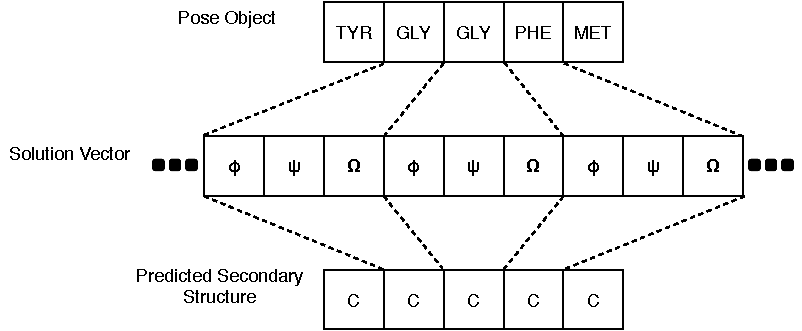
\includegraphics{Figuras/protein-representation.pdf}
    \vspace{1mm}
    \caption{The Protein Computational Model (Source: Author)}
    \label{fig:protein-model}
\end{figure}

The secondary structures are classified using a DSSP8
notation~\cite{frishman1995knowledge}.  For this work they were predicted using
the PSIPRED\footnote{Available for academic use in:
\url{http://bioinf.cs.ucl.ac.uk/psipred/}}  server~\cite{mcguffin2000psipred}. The knowledge from the secondary
structure prediction is incorporated in the model using fragment insertion,
which will be further explained in Section~\ref{sec:conformation-sampling}.

At the end of the prediction, the output consists of a full atom protein
representation, including the side chains. For this, an off-the-shelf repacker
available in Rosetta toolkit was utilized.  The repacker replaces the
ellipsoids with the actual side chains. This introduces a series of (potential)
hysterical clashes between the side chains, specially in more densely packed
structures. To solve this problem, a gradient descent optimization is
performed, where the Van der Waals repulsive forces are slightly varied during
the gradient descent.  With this, the gradient descent can rotate the side
chains and move the backbone in order to make room for the newly inserted side
chain structures.  The final result of this is a full atom representation of
the predicted protein, which is the output of the proposed approach.

\section{Energy Functions Employed}
\label{sec:energy-function}

The energy function represents the domain information from the \ac{PSPP} in a
mathematical equation. Different energy functions considers different aspects
of the problem, which can be useful for different steps of the prediction. This
work makes use of three energy functions available in Rosetta.

The first energy function utilized is referenced in Rosetta as score0. This
energy function consists solely of the repulsive Van der Waals forces. The goal
of this energy is to aid the generation of initial conformations. Since only
the repulsive forces are considered, a score0 with a value of $0$ indicates
that a given conformation has no clashes between different parts of the
protein. The assembly of the protein guided by the score0 function leads to
more plausible starting proteins.

The second energy function utilized is referenced in Rosetta as score3. It uses
a full atom representation of the backbone and an ellipsoid to represent the
side chains. A more in depth explanation of this energy function is explained
in~\cite{alford2017rosetta}. Unfortunately, the only up to date documentation
found for the energy functions is the Rosetta source code itself.  The score3
energy function is used during the main portion of the prediction process
described next section.

Finally, the last energy function is the scorefxn, as found in Rosetta. It
encompasses the same information as score3, however, it considers a full atom
representation of the side chain as well. This energy function is utilized
during the last step of the prediction in order to output a full atom
representation of the protein.

\section{Conformation Sampling}
\label{sec:conformation-sampling}

% Given the computational complexity of the problem, exact search procedures are
% not fast enough. Therefore, due to its limitations,
% metaheuristic methods must be employed in order to search for good results
% in a reasonable amount of time.
Many metaheuristics can be employed
on the \ac{PSPP}, as shown in Section~\ref{sec:bioinspired}
For this work, an Evolutionary Algorithm is employed due to its capability
of easily integrating with the necessary tools,
% while having the required level of performance.
while being able of detecting promising regions in the search landscape of the
problem. Furthermore, to increase
its performance, and online parameter control technique will be
utilized based on the \ac{SaDE} framework~\cite{qin2005self,qin2009differential}.
Since this work does not use any of the operators from \ac{DE}, from now on
\ac{SaDE} will be referenced as \ac{SaEA}, with the goal of clarifying
and reinforce that the proposed method in use does not rely on \ac{DE}.
Nevertheless, regarding online parameter control, \ac{SaDE} and \ac{SaEA}
are all the same.

In~\cite{kim2009sampling} is stated that the bottleneck of solving the
\ac{PSPP} is the conformation sampling procedure. Therefore, it is the part
that must be more focused on, since increasing its performance will likely lead
to better predictions. Furthermore, a blind optimizer that has no knowledge
about the problem domain can inherently have a worse performance, since it will
spent more time sampling regions of the conformation space that are not
biologically plausible. Thus, having an efficient sampling procedure and
utilizing problem domain knowledge is important and can possibly lead to a
better predictor.

The domain specific operator utilized in this work consists of
fragment insertion. Four fragment insertion operators are employed.
Two classic fragment insertion operators of size 3 and 9 are utilized
as well as two smooth fragment insertions of size 3 and 9.

The classic fragment insertion can be considered a global search
operator, as it leads very often to very impactful changes
in the conformation. Due to the proportions of these changes,
this operator will have a decreasing chance of making a move
that can improve the current solution as the optimization process
progresses.

The smooth fragment insertion on the other hand can be thought as
being a local search operator. The nature of this operator
is to try to negate the changes of the first fragment insertion by using
a second one specially localized. This leads to smaller changes on the
overall protein conformation, even though twice the residues are changed.
The use of this operator allows for \ac{SaEA} to have a domain specific local
search, which stays effective over the whole optimization process.

These four fragment insertion operators require a criteria to be used. For
this, a \ac{MC} based search is employed. Two different Monte Carlo based
approaches are utilized. The first being a simple \ac{MC} search, where
\ac{SaEA} selects one of the four fragment insertion operator and runs a small
(less than 100 iterations) batch of insertions. The other procedure consists of
a Replica Exchange Monte Carlo (REMC). In \ac{REMC} either a fragment is
inserted or the whole conformation is exchanged with another conformation
previously analyzed. This exchange happens also under the Metropolis criteria.
That is, a good conformation will always be accepted while a worse has a
inversely proportional change of being accepted based on how worse it is.  The
use of \ac{REMC} allows for a good conformations to be explored more while bad
ones will have a chance of being ignored. Since the Metropolis criteria will
always favor the better conformation, \ac{REMC} could lead to a very fast
premature convergence, where it would replicate the same conformation to all
solution vectors.  In order to avoid this, a ring topology is utilized. The
$i$-th conformation can only compete with the $i-1$-th conformation, and the
first one with the last. This adds a latency for the best conformation to
replace all the others, giving a chance of another good conformations being
found.

Another important tool in the conformation sampling step is the \ac{FFI}.
\ac{FFI} consists of inserting a random fragment regardless of its impact. That is,
differently from the \ac{MC} fragment insertion, \ac{FFI} applies the fragment
without taking into account the energy impact that it has. This in effect has
two direct consequences. Firstly it has the potentially bad action that it can
destroy good conformations. On the other hand, it can also escape from local
minima, therefore, increasing the sampling efficiency.

Determing when \ac{FFI}
occurs is of paramount importance. If it happens often, good conformations will
keep being destroyed and the sampling procedure will be impaired. If it seldom 
happens, then the benefit of escaping local minima will rarely be used. Therefore,
the strategy has to be tuned in a way that we escape local minima often enough
to avoid wasting too many function evaluations while not destroying too many
good conformations. In addition, exploring local minima is by itself import.
While the optimization is happening, there is no way of knowing if the best local
minima found so far is the global minima or not. So, if local minima are not
explored enough, it is possible that \ac{FFI} prevents the optimal point from
being found.

Despite its potential downsides, using \ac{FFI} can help prevent premature
convergence in the system. It adds diversity to conformation pool in a controlled
manner. With that, a constant stream of information is added to the optimizer.
Finally, coupled with the optimizer itself, \ac{FFI} acts as a catalyst for the
optimizer to be able to do big changes in the conformation, because \ac{FFI} can
bypass the greedy nature of the \ac{EA} utilized.

Figure~\ref{fig:search-procedure} presents a flowchart of the proposed
approach. It is split into three main steps: The initialization phase, the
optimization phase and post processing phase. These three steps assemble the
predictor as a whole.

\begin{figure}
    \centering
    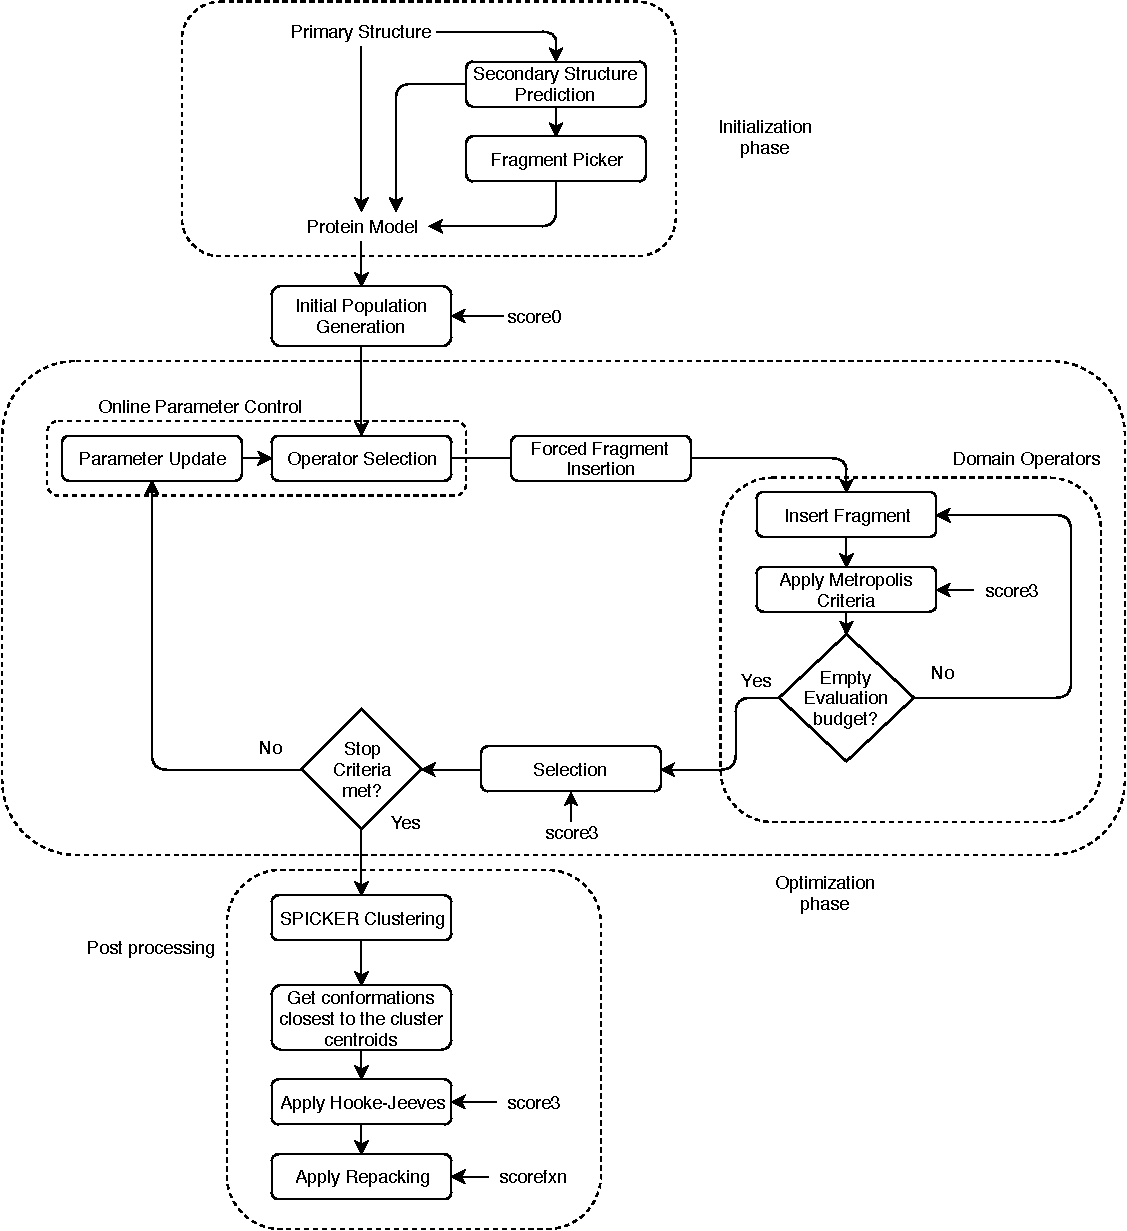
\includegraphics[width=\linewidth]{Figuras/search-procedure.pdf}
    \caption{The Proposed Search Procedure (Source: Author)}
    \label{fig:search-procedure}
\end{figure}

In the initialization phase the primary sequence is taken as input in the FASTA
format, which consists of the one letter code sequence of amino acids. The
primary sequence is then stored for later use. It is also used as input for
PSIPRED, the secondary structure predictor. PSIPRED outputs a probability
matrix mapping probabilities for the cartesian product of secondary structures
versus the amino acid sequence. This output is also stored for later use and is
fed into the fragment picker.  The fragment picker used is the Rosetta Fragment
Picker and it is responsible for selecting a set of fragments for all possible
combinations of contiguous amino acids of size 3 and 9. The fragment set is
stored to be used as input for tertiary prediction routine. Since the
initialization phase consists only of preprocessing, its time is not taken into
account when measuring the time required to predict a given target protein.
Specially considering the waiting time for the PSIPRED server.

The second phase is the optimization phase.  It starts with the step of
generating the initial population. The initial population generation consists
of assembly random protein conformations using the fragments generated in the
initialization phase. A Monte Carlo search is ran using the score0 energy
function in order to search for protein conformations that have no (or as few
as possible) hysterical clashes. This step stops when a fixed number of samples
is used for each solution vector in the population or when the score0 function
reaches zero.

With the initial population generated, the optimization procedure itself starts
guided by the score3 energy function. The basis of the search procedure is
carried out by the \ac{SaEA} algorithm, which consists of the \textit{Online
Parameter Control} part without the \textit{Differential Evolution Operators}.
The hybridization happens when the \textit{Domain Operators} are added to the
search procedure.

Firstly, the online parameter control portion of \ac{SaEA} selects which
operator to use for each individual in the population.
%
The operators can be either \ac{MC} or \ac{REMC}, with different fragment sizes.
Once it is selected, a small sub search procedure starts, corresponding to the
operator itself.
%
Before the operator is applied, the check for \ac{FFI} happens. The check occurs
for all solution vectors. If the \ac{FFI} check passes, then a random fragment
is applied. Regardless of \ac{FFI} being used or not, the next step is to apply
the standard fragment insertion.
%
A \ac{MC} or \ac{REMC} search procedure is initialized,
based on the operator chosen. This search takes a fixed amount of function
evaluation that is fed as a parameter. When this search procedure stops the
output is fed to the selection routine. From there it is checked if the stop
criteria was met. If it was not, then the parameter update routine is called,
updating the parameter Cr (for all operators) as well as the
probabilities for each operator. Since \ac{DE} is not used, the $Cr$ parameter
actually controller the \ac{MC} temperature parameter. The parameter control is
agnostic to which parameter it is updating. Once the Parameter Update step is
finished, the optimization cycle starts over again from the operator selection.

The when stop criteria is ultimately met, the optimization phase stops and the
post processing phase starts. The first post-processing step is to cluster the
conformations. After the clustering process finishes, the cluster centroids are
selected. The number of clusters are a parameter of the algorithm.
The conformations closest to the centroids are found and feed forward
to the next steps, while the centroids themselves are discarded. A Hooke-Jeeves
local search is applied. This helps to reach nearby local minima that might have
been inaccessible by the fragments alone. Once the local search finishes, the
repacking procedure is applied to all the conformations that were selected in
the clustering phase and then re-optimized. The repacking procedure removes the
centroids and places rotamers (side-chains fragments). The conformation is again
re-optimized, this time using a gradient descent guided by the scorefxn energy
function. After this step finishes the conformations are returned. Returning
the conformation nearest to each centroid (and re-optimizing/repacking it) allows
for a human specialist to inspect multiple conformations that are apart from
each other and select the best one. In this way, one run can provide multiple
potentially useful solutions.

Two variant of this algorithm exist. One using \ac{MC} for the fragment insertion
and the other using \ac{REMC}. It is expected that the \ac{MC} variant will have
a bigger overall diversity, and thus, returning conformations that are more
different apart. Meanwhile, the \ac{REMC} variant is expect to exploit more at
the expense of conformation diversity. That is, it may get stuck in a local
minima more easily in exchange for a increased chance of finding a better solution.
The first method is named SADE-MC-FINAL and the second is named SADE-REMC-FINAL.
\chapter{Experiments, Results and Analysis}\label{chap:experiments_and_results}

% Present the chapter
In this Chapter, the results are presented and a rigorous
analysis is realized. In Section~\ref{sec:design_of_experiments}
the design of experiments is presented, where the outlines of how
and where the experiments were executed is explained. The methodology
for comparison is also discussed in that section. In
Section~\ref{sec:methods-analysis} a rigorous set of statistical
tests is presented and applied to the results, with the goal of
comparing the proposed methods against references in the literature.
The genotipic and fenotipic diversity of the two proposed method is
inspected and analysed in~\ref{sec:convergence-analysis}.
An analysis of the two proposed methods is presented in
Section~\ref{sec:methods-duel}, where it is verified if there is one with a
superior performance and which one.
In Section~\ref{sec:repacking-impact} an analysis of the impact that
repacking has on the proposed methods is presented. This, compares how
the RMSD and energy, relative to rosetta, changed when repacking was
applied. This section has two goals. First, to identify if repacking
did or did not influence the results from the statistical tests.
Secondly, to document its impact.

The processing time required to run the proposed methods is exposed in
Section~\ref{sec:time-and-evals}, along with the number of spent function
evaluations. Then, in Section~\ref{sec:competing-methods} an in depth
analysis of the two proposed methods is presented, where they are
compared versus more than 20 works in the literature.
Section~\ref{sec:other-metrics} presents an analysis using GDT-TS
and TM-Score, with the aim of providing further insight on the results.
Furthermore, the raw data from the experiments is also provided with
the object of allowing further works to more easily compare with the
presented methods. A visual analysis of the best conformations is
presented in Section~\ref{sec:visual-analysis}, where some of the
prediction problems can be identified and are commented.

\section{Design of Experiments}\label{sec:design_of_experiments}

% Present the hardware setup
The experiments were all conducted on a single machine using the same hardware
throughout the full experimentation. Table~\ref{tab:machine-setup}
presents the machine utilized to run all the experiments. Each run of a
prediction method consists of a serial program that run continually without
interruption. The experiments were run in parallel, limited to at most one
running test per core\footnote{Only physical cores were considered. No virtual
(Hyper-threading) core was involved in the computations.}. To ensure maximum
repeatability the machine had no graphical interface enabled or any other form
of user interaction during the course of the experimentation.

\begin{table}[th]
    \centering
    \begin{tabular}{r|l} \hline \hline
        Name & Value \\ \hline \hline
        Operating System & Arch Linux \\ \hline
        Kernel &  Arch Linux Kernel 4.18.16 \\ \hline
        CPU & Intel(R) Core(TM) i5-3570K CPU @ 4.20GHz \\ \hline
        Number of Cores & 4 Physical cores, no hyper-threading cores \\ \hline
        RAM & 16 GB @ 1400 MHz \\ \hline \hline
    \end{tabular}
    \caption{The Machine Setup}
    \label{tab:machine-setup}
\end{table}

The experimentation consisted of running the two proposed methods, namely
PPF-REMCc and PPF-MC. One of the methods proposed
in~\cite{silva2019self} is also included, namely SADE-REMC.
Lastly, the Rosetta Ab Initio protocol is also included, amounting to four
different methods being ran.

The analysis is divided in two steps. In the first one, the two proposed methods
are compared against the work from~\citeonline{silva2019self} and the Rosetta Ab Initio
Protocol.
Rosetta was selected as an representative of the state of art,
while the other method, SADE-REMC, is a precursor of the two proposed methods.
Since there is open
access to both methods, it is possible to run and analyze experiments with them
more easily and to do a direct statistical analyse on the results.

% Present the "in house" comparison
The metrics utilized are the \textit{scorefxn} energy value of the
best solution and the \ac{RMSD} associated with the this conformation. The
results were collected over 50 independent runs of each method for each target
protein. A graphical analysis is conducted in order to identify visually the
relative performance between the proposed methods. Considering that a visual
analysis is not enough (in this case), a more rigorous numerical statistic set
of test is conducted. The Shapiro-Wilk~\cite{wilk1968joint} normality test is
employed with a confidence level of 5\%, i.e. $\alpha = 0.05$, to assess the
presence (or lack) of an underlying normal distribution. Based on its result, a
parametric/non-parametric test is employed with a confidence level of $\alpha =
0.05$. Due the presence of multiple comparisons, the Kruskal-Wallis test is
applied in order to detect if there is any method with a performance that
is different than the others. If there is, then, the pairwise Mann-Whitney test is
employed with the proposed methods against its competitors.

% Explain the clustering results
The use of clustering to extract and return different conformations from the
proposed methods is highly important in a complex and extremely multi-modal
problem such as the PSPP. With clustering, it is possible to identify conformations
that are far apart from each other in the energy landscape, however, that have
similar energies. This process require extra steps during the analysis.
First, the main use of
returning several conformations is to allow an human expert to choose one that
has the desired properties. This, can not be automated in a test environment where
hundreds of experiments are performed computationally each day. As such, the human
expert, for the purposes of performance evaluation, must be replaced by a
computer oracle. This oracle can always find the conformation with the lowest
RMSD or the conformation with the lowest energy. This, of course, would not
be possible in a real world scenario where a protein without a known structure is
being predicted. With that in mind, the analysis of the two proposed methods is
divided in two sub groups. The first is named \texttt{best-by-rmsd} and the second
is named \texttt{best-by-energy}.

% Present the "free for all" analysis
In the second analysis step, a direct comparison against several works in the
literature is considered. Since there is a severe lack of standardization in the
literature regarding experimentation, the following methodology was used. Works
that provided the best RMSD had their proteins listed. The proteins that occurred
the most were used for comparison. It is worth noting that the majority of works
provide little information about how the experimentation was conducted. The way
in which the results are analysed lacks a standard. As such, this work does a
direct comparison using the best RMSD achieved in a set of runs. While this is
not ideal, due to different works running each method different number of times,
this is possibly the only way to a comparison against several works. %The presence of outliers also weaken this comparison. Also, since only the most used proteins are select, it is possible that some works are only represented partially, i.e. some of the results are left out. 
Nevertheless, at the end of the day for the PSPP what matters is having the lowest possible error. As such, comparing the best RMSD is a worthwhile analysis. %, albeit not ideal.

% Present the protein set
With that in mind, the set of proteins presented in Table~\ref{tab:protein-targets}
was chosen. The column \textbf{Name} contains the protein identification code
as in PDB.  The \textbf{Size} column shows the number of amino acids in the protein.
The \textbf{Backbone Angles} column shows the number of angles in the backbone,
this also has a one to one relation to the number of variables to be optimized
for a given protein. The \textbf{Structure} column holds the secondary
structures present in the protein set represented by $\alpha$-helices or
$\beta$-sheets.

\begin{table}[bh]
  \centering
  \begin{tabular}{ l | c | c | c | c }
    \hline \hline
    Name & Size & Backbone Angles & Structure         \\ \hline \hline
    1l2y & 20   & 60              & $2\alpha$         \\ \hline
    1wqc & 26   & 78              & $2\alpha$         \\ \hline
    1acw & 29   & 87              & $1\alpha, 2\beta$ \\ \hline
    1zdd & 35   & 105             & $2\alpha$         \\ \hline
    2mr9 & 44   & 132             & $3\alpha$         \\ \hline
    1crn & 46   & 138             & $2\alpha, 2\beta$ \\ \hline
    1enh & 54   & 162             & $3\alpha$         \\ \hline
    1rop & 63   & 189             & $2\alpha$         \\ \hline
    1utg & 70   & 210             & $4\alpha$         \\ \hline
    1ail & 72   & 216             & $3\alpha$         \\ \hline
    \hline
  \end{tabular}
  \caption{Target proteins and their features}
  \label{tab:protein-targets}
\end{table}

% Present the parameters
The two proposed methods all operates with the same parameters, as presented
in Table~\ref{tab:parameters}. The first column contains the parameter name and the
second one its respective value.
Population Initialization refers to the \ac{MC} search that is made using
\texttt{score0}. It has $10000$ function evaluations available, such that up to
$100$ are used for each solution vector.
The SaDE learning Phase has its default value,
as presented in~\cite{qin2009differential}. There are 100 simultaneous
trajectories throughout the execution, i.e. a population size of 100. A million
function evaluations are available for the optimization phase, where each
fragment insertion routine can use up to 25 at a time. \ac{FFI} uses a fragment
size of 9 and is applied with a probability of 2\% before each standard fragment
insertion. The other methods being compared use the same values from
Table~\ref{tab:parameters} as applicable.

\begin{table}[ht]
    \centering
    \begin{tabular}{r|l} \hline \hline
        Parameter & Value \\ \hline \hline
        Population Initialization Evaluation Budget & 10000 \\ \hline
        SaDE learning Phase & 50 \\ \hline
        Population Size & 100 \\ \hline
        Function Evaluation Budget & 1000000 \\ \hline
        MC/REMC Function Evaluation Budget & 25 \\ \hline
        Spicker cluster size & 10 \\ \hline
        \ac{FFI} probability & 0.02 \\ \hline
        \ac{FFI} length & 9 \\ \hline \hline
    \end{tabular}
    \caption{Parameters utilized in the proposed methods}
    \label{tab:parameters}
\end{table}

\section{Energy and RMSD Analysis}\label{sec:methods-analysis}

% Introduce the analysis
Due to the amount of data generated by the experiments, most of the analysis will
be conducted by visual inspection or by summarizing the results and key-points.
However, for the sake of completude and scientific rigor, complementary
information is provided in Appendix~\ref{appendix:table-results}.
Moreover, the analysis is divided in three main parts. In the first part, a visual
analysis using boxplots is used in order to observe the overall performance of
the proposed methods. Following, a statistical framework is used to assess the methods
performance relatively to each other. Then, a Pareto front analysis is presented
using the best results from the four methods.
% In
% Section~\ref{sec:statistical-analysis} a strictly statistical analysis is
% presented. Section~\ref{sec:pareto-front-analysis} presents an analysis of the
% best results achieved using Pareto Front.

% Present the box plots
In Figure~\ref{fig:boxplot-rmsd} the RMSD from the predictions is presented as box-plots.
The proteins, presented in the x-axis, are displayed in lexicographical order.
The y-axis presents the RMSD, where lower is better. The methods are grouped
horizontally by protein.

It is possible to verify that for 9 out of 10 proteins (with exception for 1rop) the
two proposed methods, in orange and green, had a very close overall performance,
considering the median, presented as the line inside the box of each method.
For 1rop, the PPF-MC outperformed the other methods by a significant margin.
Moreover, the two proposed methods had better medians than
the other methods (not including rosetta) in 8 of the 10 proteins,
with exception for 1rop and 1zdd.
For 1rop, the SADE-REMC had the second best result, behind PPF-MC, while PPF-REMC
had the worst result.
For the 1zdd protein, the two proposed methods had the two worst
medians, however, by a relatively small amount.

In a direct comparison against rosetta, proteins 1acw, 1enh, 1l2y, 1utg and 2mr9
the proposed methods had a significant improvement upon rosetta.
For 1crn the rosetta appears to have had
a slightly better performance compared to the proposed methods.
In the remaining proteins, 1ail, 1rop, 1wqc and 1zdd, it is not
possible to visually detect in a objective manner if there was
a significant performance improve. This, will be address later with statistical
tests.
% visual inspection is not enough to accurately detect significant performance differences.

Some other behaviours are worth noting. The manifestation of each
proteins uniqueness is visible in the distribution of different methods. For example,
a simple visual inspection on Figure~\ref{fig:boxplot-rmsd} shows that on
2mr9, rosetta had a worst performance than the other methods by a significant margin,
whereas the other methods had a very similar performance. For 1utg, the two proposed
methods outclassed the other methods, including rosetta. Furthermore, the worst
result from PPF-REMC was better than the medians of all the other methods.
Now, interestingly, for 1wqc and 1crn, rosetta and the two proposed methods had
better performance than the other methods. Also, for some proteins, such as 1enh,
the overall performance is much closer. One possible explanation for this difference
in results, considering that all the methods had the same input, is the conformation
sampling strategy. Some strategies might best suit some proteins with a given conformation
structure more than others. All these visual observations are later confirmed with
statistical tests.

\begin{figure}
  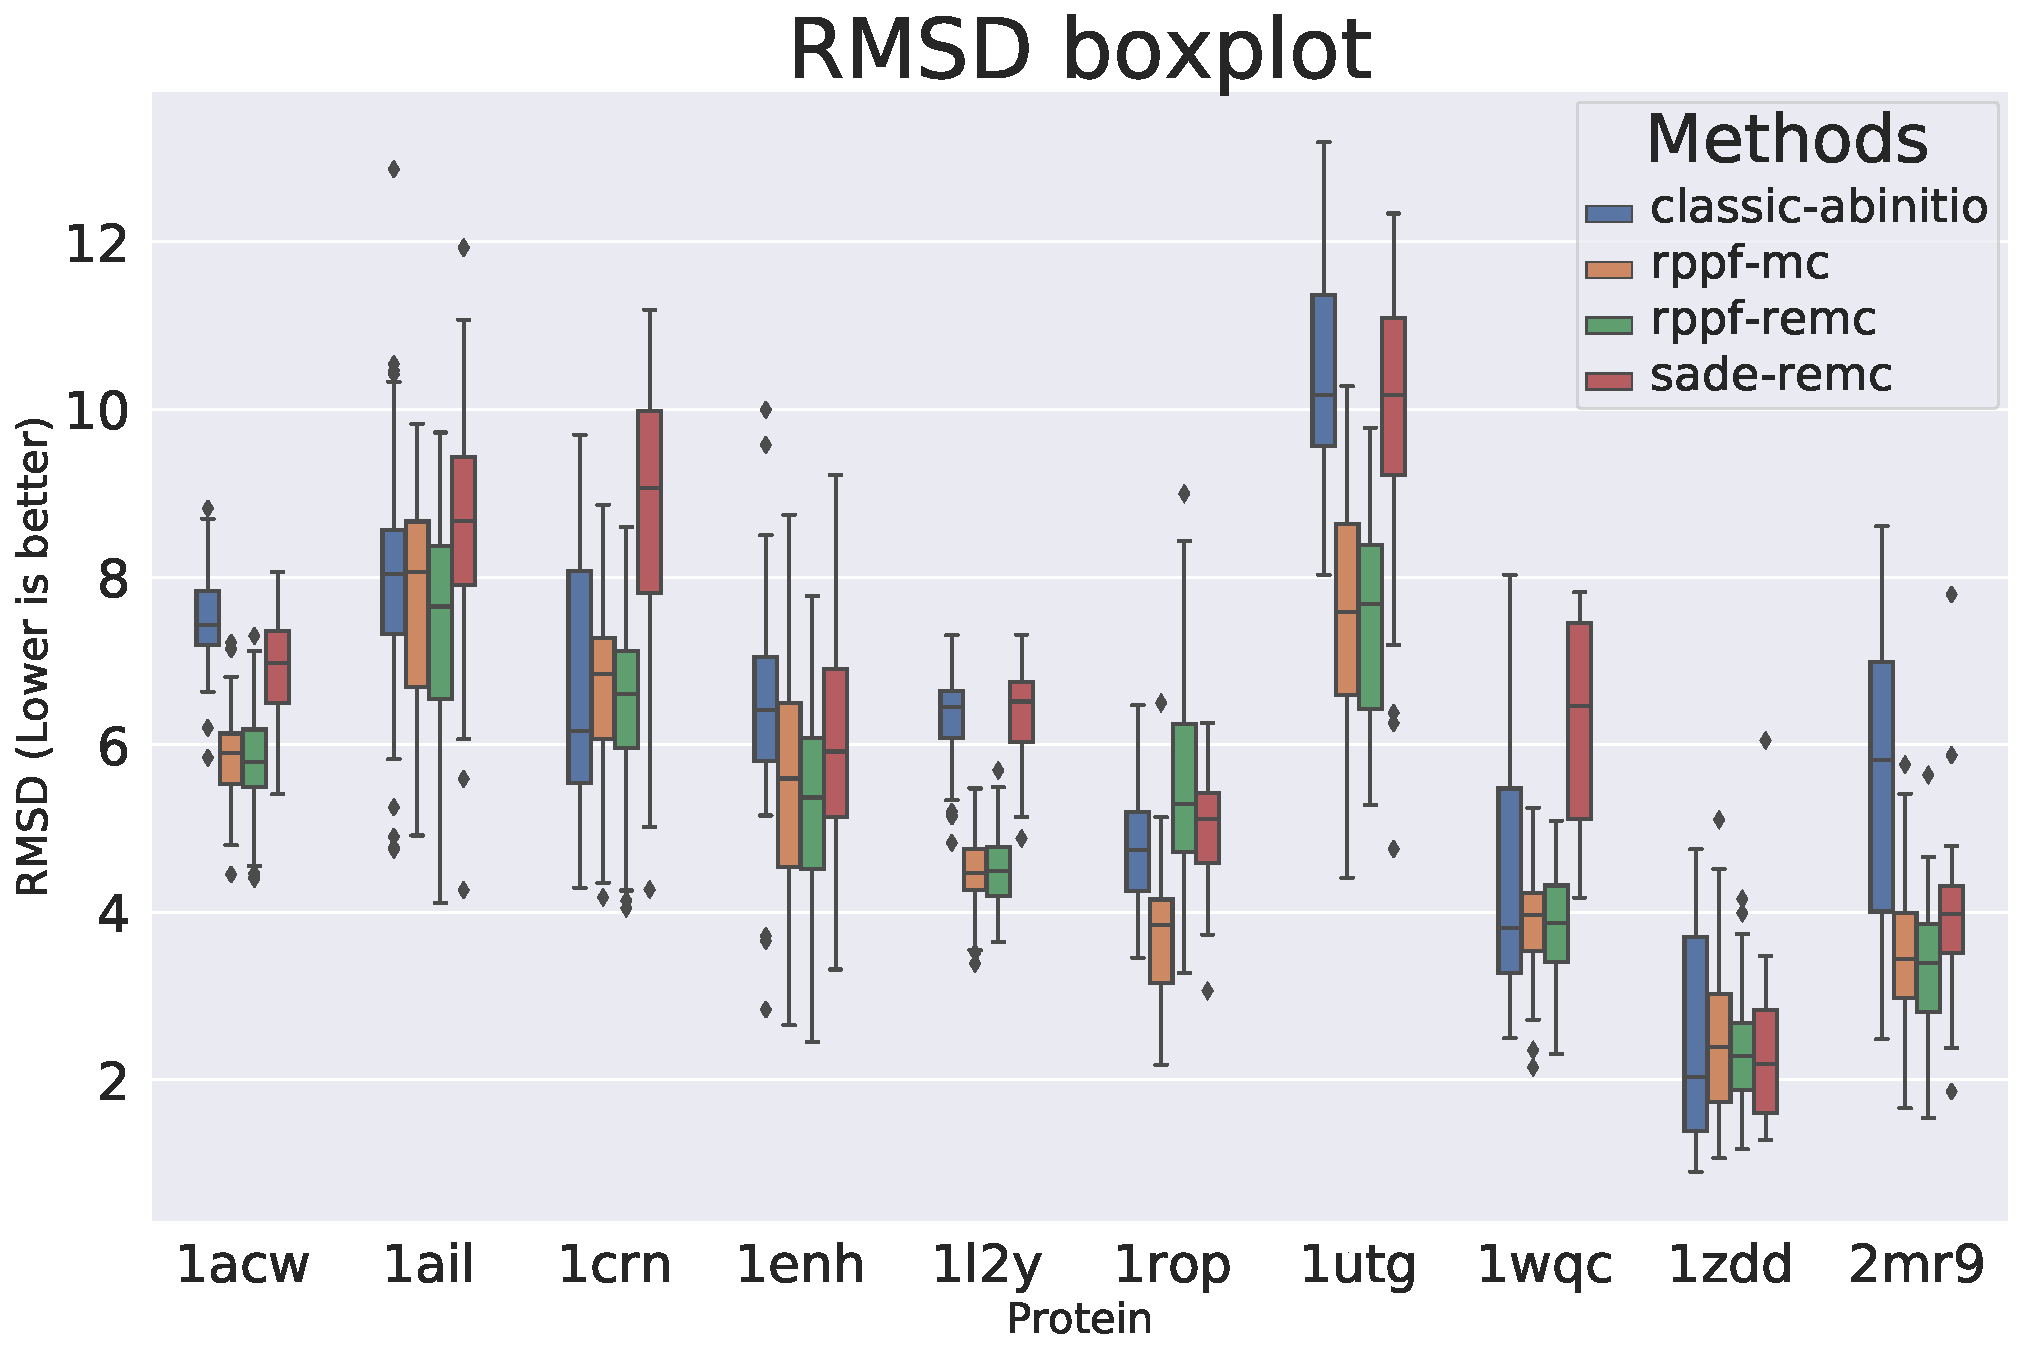
\includegraphics[width=\linewidth]{Figuras/boxplots/boxplot_best_by_rmsd_rmsd_after.pdf}
  \caption{Boxplot presenting the RMSD for the protein predictions with the
    competing methods. For the two proposed methods, the \texttt{best-by-rmsd}
    data was used}
  \label{fig:boxplot-rmsd}
\end{figure}

Figure~\ref{fig:boxplot-energy} presents data similarly to the previous figure,
however, the y-axis now represents the \texttt{scorefxn} energy function. Considering
the energy results, when compared to the rmsd boxplot, the results are relatively
more similar. Nevertheless, for some proteins there are some behaviours that are
more visible. For 1rop, PPF-REMC appears to have had a worst performance
than the other methods. Same as with the RMSD data. For 1crn, rosetta and the two
proposed methods appears to have a better overall result. For 2mr9, rosetta
appears to be lagging behind in performance. These observations are just visual
trends which helps understand the relative performance.
% In order to properly
% access their differences a more rigorous statistical approach is required and exposed next.

\begin{figure}
  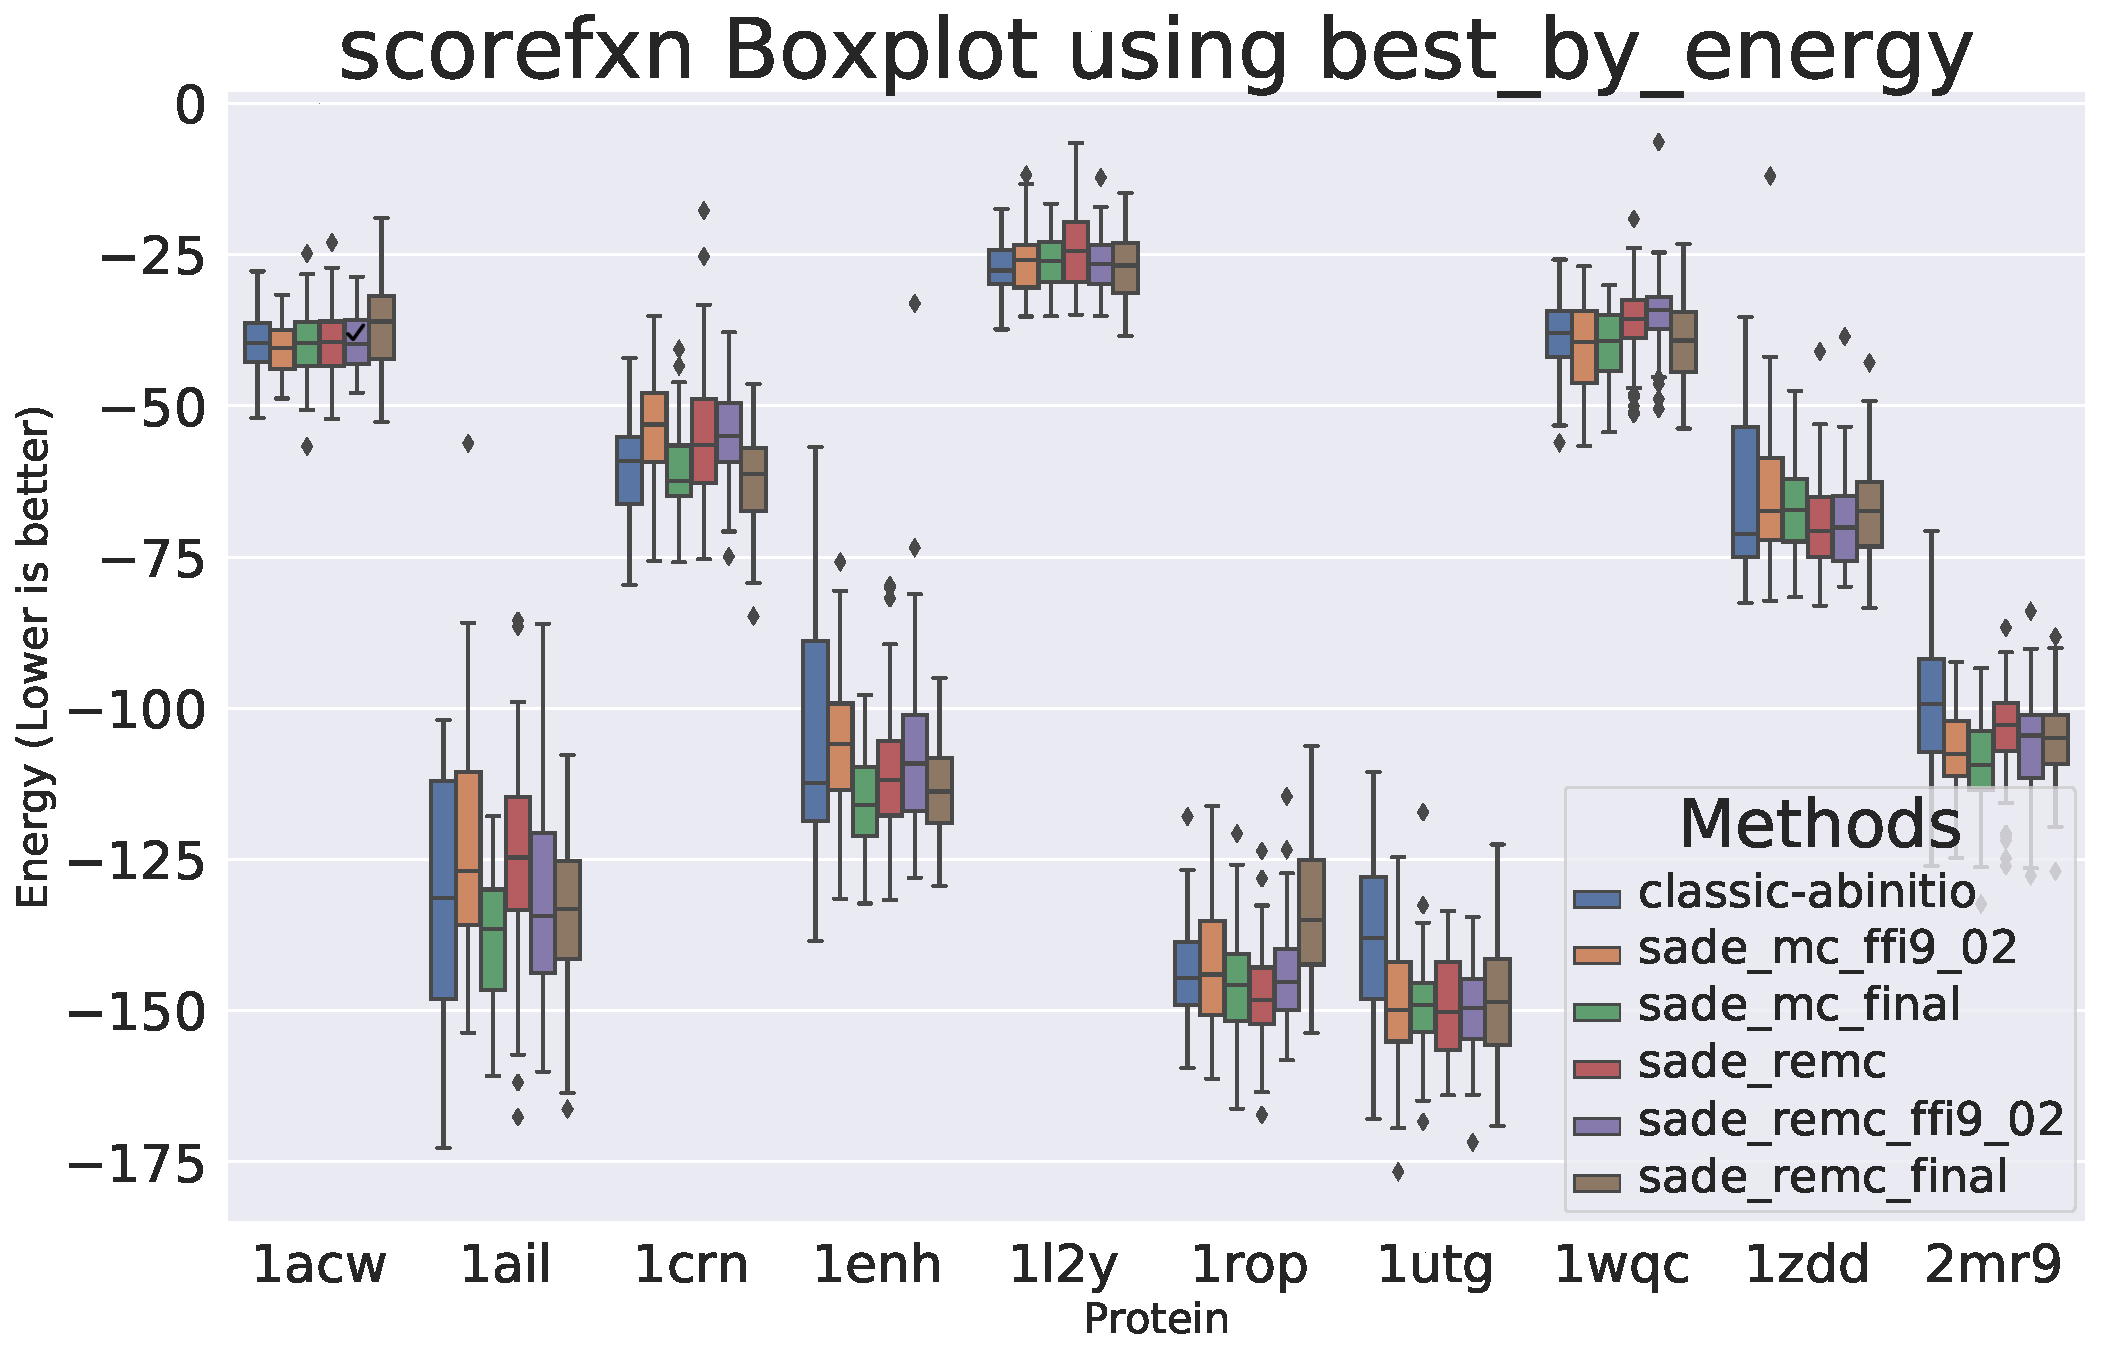
\includegraphics[width=\linewidth]{Figuras/boxplots/boxplot_best_by_energy_scorefxn.pdf}
  \caption{Boxplot presenting the \texttt{scorefxn} for the protein predictions with the
    competing methods. For the two proposed methods, the \texttt{best-by-energy}
    data was used}
  \label{fig:boxplot-energy}
\end{figure}

% \subsection{Statistical Analysis}
% \label{sec:statistical-analysis}

% Present Shapiro-Wilk RESULTS
To scientifically assess the performance of the proposed methods relative to
other competing methods, proper statistical tests are required. A prerequisite
before applying the tests which evaluate performance is to detect the
underlying distribution of the data to be analysed. There are several ways to
accomplish this. One, is to visually inspect a histogram or a Quantile-Quantile
plot. A more rigorous approach is to use a statistical test which can evaluate
the presence of a gaussian distribution. One such test is the Shapiro-Wilk and it
will be utilized for this purpose.

For the statistical analysis, an $\alpha = 0.05$ was utilized indicating a confidence level of 5\%. The RMSD and \texttt{scorefxn} of both the \texttt{best-by-rmsd} and \texttt{best-by-energy} were analysed for all the methods. For the sake of brevity the results are exposed outside this
text, in Appendix~\ref{appendix:shapiro}. The null hypothesis, $H_0$, is that
the samples belong to a normal distribution. Therefore, if the test returns a $p$
value less than $\alpha$, $H_0$ is rejected and the underlying distribution is
not gaussian. If $p$ is equal or bigger than $\alpha$, then the test failed to
reject $H_0$. Considering the data to be analyzed, this is not so straight
forward. There are 2 metrics to be analysed, the RMSD and \texttt{scorefxn}.
There are several methods which were executed. Furthermore, several proteins
were utilized for testing. Not only this gives a big amount of data to analyze,
it is possible that some method, protein or metric may lead to a gaussian
distribution, where others don't.

The tests were applied for RMSD and Energy, which lead to mixed results. Some
combinations of methods and proteins had gaussian distributions while others did
not. Considering this, both Kruskal-Wallis and Mann-Whitney tests can deal with
both gaussian and non-gaussian distributions with little cost of accuracy.
%
% For the RMSD using \texttt{best-by-rmsd}, there were $37$ cases where $H_0$
% failed to be rejected, and $23$ where it was rejected. All methods when applied
% to protein 1acw gave a gaussian distribution. For 1zdd, 5 of the 6 methods gave
% a non-gaussian distribution. The proteins, 1crn, 1l2y and 2mr9, had split results
% where half the methods rejected $H_0$ and half didn't. Some proteins appear to
% be more propense to generate gaussian distributions than others. By analysing
% the methods instead of the proteins, a new insight is given. The two proposed
% methods had $2$ and $1$ rejection of $H_0$, for PPF-MC and PPF-REMC,
% respectively. Whereas sade-mc-ffi and SADE-REMC both had $6$ rejections. This
% indicates that some methods are more propense to generate gaussian distribution
% than others.
% 
% Considering \texttt{scorefxn} with \texttt{best-by-energy}, there were $46$
% cases where $H_0$ failed to be rejected, and $14$ were it was rejected. On this
% situation, with the given metric, more methods are generating gaussian
% distributions. Three proteins, 1acw, 1crn and 1l2y, failed all times to reject $H_0$.
% For 1ail and 1enh, the results were split in the middle. 1zdd had the most
% rejections of $H_0$, with $4$. The remaining proteins had only a single
% rejection of $H_0$. with both metrics, 1zdd had the most rejections of $H_0$,
% whereas all methods on 1acw failed to reject $H_0$. Looking at the methods,
% there is no clear trend. The proposed method PPF-REMC had no rejection
% of $H_0$, while PPF-MC had two.
%
% Conclude the analysis and introduce the next analysis
% Given this, it appears that the underlying distribution, in most cases,
% is gaussian. However, there are consistent, albeit fewer, situations where they are
% not gaussian. As such, a non-parametric test must be employed.
%
In this case, the analysis is split in two steps.
Firstly, Kruskal–Wallis test is applied in order
to detect if there is a significant difference between the distribution, i.e.
if there is a method that is better than some other. If there is, then
a pairwise Mann-Whitney is utilized. Even though it is a non-parametric test, it
has, relative to Student's t test, a similar performance. Therefore,
Mann-Whitney's test can suit the needs to analyse the data at hand. Running
Mann-Whitney only if Kruskal–Wallis detects a significant difference is
important, as it helps to prevent inference errors.

% Present kruskal-wallis RESULTS
The Kruskal–Wallis test was performed with an $\alpha = 0.05$. The null-hypothesis
is that all the samples were drawn from the same distribution, i.e. all the
methods have equivalent performance.
Table~\ref{tab:kruskal-wallis-best-by-rmsd-RMSD} presents the result of the
tests for the RMSD.
The column protein indicates the name of the protein, and the column
$p$-value indicates the result of the test. When the $p$-value is less than
$\alpha$ it is highlighted in boldface. The result if very straightforward to
interpret. All the proteins with the exception of 1zdd had a $p$-value less
than the selected $\alpha$. Moreover, when $H_0$ was rejected, the $p$-value
was less than $1e-05$ in all cases. For 1zdd, $H_0$ failed to be rejected, the
most likely reason is that since this protein is (arguably) the easiest one,
all methods reached near-native conformations.

Table~\ref{tab:kruskal-wallis-best-by-energy-scorefxn} reads the same
as the previous one, however, the data it displays regards to \texttt{scorefxn}.
Protein 1zdd failed to reject $H_0$ again, as did 1l2y, another relatively
simple and short protein. For all the remaining proteins $H_0$ was rejected.
Therefore, it is safe to do a pair-wise test using Mann-Whitney's.

\begin{table}
  \begin{minipage}{.5\linewidth}
  \centering
  \begin{tabular}{r|c}
  Protein & $p$-value \\ \hline \hline
  1acw & $\bm{0.0000}$ \\ \hline
  1ail & $\bm{0.0000}$ \\ \hline
  1crn & $\bm{0.0000}$ \\ \hline
  1enh & $\bm{0.0000}$ \\ \hline
  1l2y & $\bm{0.0000}$ \\ \hline
  1rop & $\bm{0.0000}$ \\ \hline
  1utg & $\bm{0.0000}$ \\ \hline
  1wqc & $\bm{0.0000}$ \\ \hline
  1zdd &     $0.4145$  \\ \hline
  2mr9 & $\bm{0.0000}$ \\ \hline
  \end{tabular}
  \caption{Kruskal-Wallis for \texttt{best-by-rmsd} using RMSD}
  \label{tab:kruskal-wallis-best-by-rmsd-RMSD}
  \end{minipage}
% \end{table}
%
% \begin{table}
  \begin{minipage}{.5\linewidth}
  \centering
  \begin{tabular}{r|c}
  Protein & $p$-value \\ \hline \hline
  1acw & $\bm{0.0177}$ \\ \hline
  1ail & $\bm{0.0000}$ \\ \hline
  1crn & $\bm{0.0000}$ \\ \hline
  1enh & $\bm{0.0001}$ \\ \hline
  1l2y &     $0.2930$  \\ \hline
  1rop & $\bm{0.0000}$ \\ \hline
  1utg & $\bm{0.0000}$ \\ \hline
  1wqc & $\bm{0.0001}$ \\ \hline
  1zdd &     $0.1558$  \\ \hline
  2mr9 & $\bm{0.0000}$ \\ \hline
  \end{tabular}
  \caption{Kruskal-Wallis for \texttt{best-by-energy} using scorefxn}
  \label{tab:kruskal-wallis-best-by-energy-scorefxn}
  \end{minipage}
\end{table}

% Present mann-whitney RESULTS
The Mann-Whitney test was applied with $\alpha = 0.05$. The null hypothesis is
that the two distributions are equal, i.e. both methods have the same
performance. Rejection of $H_0$ indicates that one method is better than other.
Considering that both RMSD and \texttt{scorefxn} will be analyzed, each for
10 proteins, a total of $20$ tables are necessary to expose all the data. As
such, this information is exposed in Appendix~\ref{appendix:mann-whitney-rmsd}
and~\ref{appendix:mann-whitney-scorefxn}, where the first presents the data for
RMSD and the second for the energy, respectively. The results will be summarized reporting the
overall results from the test. To keep focus and simplicity, first, the two
proposed methods will be compared against the other method. Then, they will be
compared against rosetta. In both cases, the RMSD and \texttt{scorefxn} will be
considered for the analysis.

\begin{table}
  \begin{minipage}{.5\linewidth}
  \centering
  \begin{tabular}{r|r|r|r}
  Protein & Wins & Loses & Draws \\ \hline \hline
   1acw &  6 &  0 &  4 \\ \hline
   1ail &  6 &  0 &  4 \\ \hline
   1crn &  7 &  1 &  2 \\ \hline
   1enh &  4 &  0 &  6 \\ \hline
   1l2y &  6 &  0 &  4 \\ \hline
   1rop &  4 &  3 &  3 \\ \hline
   1utg &  6 &  0 &  4 \\ \hline
   1wqc &  6 &  0 &  4 \\ \hline
   1zdd &  0 &  0 & 10 \\ \hline \overtabline
   2mr9 &  3 &  0 &  7 \\ \hline
  \end{tabular}
  \caption{Summary of Mann-Whitney \texttt{best-by-rmsd} using RMSD compared agaisnt the previous methods}
  \label{tab:mann-whitney-summary-internal-best-by-rmsd-RMSD}
  \end{minipage}
%\end{table}
%
%\begin{table}
  \begin{minipage}{.5\linewidth}
  \centering
  \begin{tabular}{r|r|r|r}
  Protein & Wins & Loses & Draws \\ \hline \hline
   1acw &  1 &  4 &  5 \\ \hline
   1ail &  5 &  1 &  4 \\ \hline
   1crn &  6 &  0 &  4 \\ \hline
   1enh &  5 &  0 &  5 \\ \hline
   1l2y &  1 &  0 &  9 \\ \hline \overtabline
   1rop &  1 &  4 &  5 \\ \hline
   1utg &  0 &  0 & 10 \\ \hline
   1wqc &  4 &  0 &  6 \\ \hline
   1zdd &  0 &  3 &  7 \\ \hline \overtabline
   2mr9 &  3 &  2 &  5 \\ \hline
  \end{tabular}
  \caption{Summary of Mann-Whitney \texttt{best-by-energy} using scorefxn compared agaisnt the previous methods}
  \label{tab:mann-whitney-summary-internal-best-by-energy-scorefxn}
  \end{minipage}
\end{table}

Starting with the RMSD using \texttt{best-by-rmsd}, comparing the two proposed
methods against the ones from a previous work, SADE-REMC, the results are shown in
Table~\ref{tab:mann-whitney-summary-internal-best-by-rmsd-RMSD}. The column
Protein displays the protein name.
Columns \textbf{Wins}, \textbf{Loses} and \textbf{Draws} show the number of
times that any of the two proposed methods outperformed, were outperformed,
or had the same performance than SADE-REMC (not including rosetta).
Based on the results from Kruskal–Wallis, as show in
Tables~\ref{tab:kruskal-wallis-best-by-rmsd-RMSD} and
Tables~\ref{tab:kruskal-wallis-best-by-energy-scorefxn}, there is no
difference between the methods for protein 1zdd both when considering RMSD and
\texttt{scorefxn}. For 1l2y also there is no difference, however, only with
\texttt{scorefxn}. As such, these rows in the table should be ignored.
These proteins are marked with an strike-through line in the following tables.

For all but two proteins, namely 1zdd and 1rop, the two proposed methods outperformed SADE-REMC.
On 1zdd, the three methods had statistically equivalent performance. For
1rop, SADE-REMC was able to outperform PPF-REMC. Going back to the boxplots,
this was expected. Interestingly, for 1rop, PPF-MC outperformed SADE-REMC, which means
that PPF-MC also outperformed PPF-REMC.

The summary concerning the energy of the conformations is show in
Table~\ref{tab:mann-whitney-summary-internal-best-by-energy-scorefxn}. It
reads the same as the table before.
For proteins 1ail, 1crn, and 1wqc the proposed methods both outperformed
SADE-REMC. On 1acw, SADE-REMC outperformed PPF-REMC and was statistically
equivalent to PPF-MC. For 1enh only PPF-MC outperformed SADE-REMC. For 1rop
SADE-REMC outperformed PPF-REMC. The only situation so far where all the
methods had statistically equivalent performance, without counting the results
from Kruskal–Wallis, was on 1utg and 1zdd.
Interestingly, on 1l2y, Mann-Whitney detected performance differences, disagreeing with
the results from Kruskal–Wallis. Nevertheless, for these protein, the result
from Kruskal–Wallis will be considered to be the correct one.

\begin{table}
  \begin{minipage}{.5\linewidth}
  \centering
  \begin{tabular}{r|r|r|r}
  Protein & Wins & Loses & Draws \\ \hline \hline
  1acw &  2 &  0 &  0 \\ \hline
  1ail &  1 &  0 &  1 \\ \hline
  1crn &  0 &  1 &  1 \\ \hline
  1enh &  2 &  0 &  0 \\ \hline
  1l2y &  2 &  0 &  0 \\ \hline
  1rop &  1 &  1 &  0 \\ \hline
  1utg &  2 &  0 &  0 \\ \hline
  1wqc &  0 &  0 &  2 \\ \hline
  1zdd &  0 &  0 &  2 \\ \hline \overtabline
  2mr9 &  2 &  0 &  0 \\ \hline
  \end{tabular}
  \caption{Summary of Mann-Whitney \texttt{best-by-rmsd} using RMSD compared agaisnt rosetta}
  \label{tab:mann-whitney-summary-rosetta-best-by-rmsd-RMSD}
  \end{minipage}
%\end{table}
%
%\begin{table}
  \begin{minipage}{.5\linewidth}
  \centering
  \begin{tabular}{r|r|r|r}
  Protein & Wins & Loses & Draws \\ \hline \hline
  1acw &  0 &  1 &  1 \\ \hline
  1ail &  1 &  0 &  1 \\ \hline
  1crn &  0 &  0 &  2 \\ \hline
  1enh &  1 &  0 &  1 \\ \hline
  1l2y &  0 &  0 &  2 \\ \hline \overtabline
  1rop &  0 &  1 &  1 \\ \hline
  1utg &  2 &  0 &  0 \\ \hline
  1wqc &  0 &  0 &  2 \\ \hline
  1zdd &  0 &  0 &  2 \\ \hline \overtabline
  2mr9 &  2 &  0 &  0 \\ \hline
  \end{tabular}
  \caption{Summary of Mann-Whitney \texttt{best-by-energy} using scorefxn compared agaisnt rosetta}
  \label{tab:mann-whitney-summary-rosetta-best-by-energy-scorefxn}
  \end{minipage}
\end{table}

In Table~\ref{tab:mann-whitney-summary-rosetta-best-by-rmsd-RMSD} the
two proposed methods is compared against Rosetta using RMSD. For 1acw, 1enh, 1l2y, 1utg and 2mr9, totalling 5 proteins, both
proposed methods outperformed rosetta. For 1ail only PPF-REMC
outperformed rosetta. On 1rop, PPF-MC outperformed rosetta, while
PPF-REMC was outperformed. On 1crn, only PPF-MC was outperformed
by rosetta. From this, it is demonstrated that both the proposed methods
consistently outperform rosetta. In fact, rosetta outperformed the proposed
methods only in 2 occasions when considering the RMSD.

The comparison of rosetta and the proposed methods using \texttt{scorefxn}
is presented in Table~\ref{tab:mann-whitney-summary-rosetta-best-by-rmsd-RMSD}.
For this particular case, for 2 proteins, 1utg and 2mr9, both proposed
methods outperformed rosetta. On 1acw and 1rop rosetta outperformed only
PPF-REMC. On 1ail, only PPF-MC outperformed rosetta. Overall,
the proposed methods outperformed rosetta in some cases and had equal
significance in others.

In light of these observations, it is safe to consider that the two proposed
methods outperform the SADE-REMC. It also outperforms rosetta, one of
the state of the art methods in the literature and CASP winners.

\subsection{Pareto Front Analysis}\label{sec:pareto-front-analysis}

In this Section an analysis of the Pareto front of the four methods under
analysis is presented.
Considering that the end user would most likely only be
interested in the best prediction, this analysis considers the conformation with
the best RMSD and its respective energy, taken from all the runs of all methods under
analysis.

\begin{figure}
  \begin{subfigure}{0.49\linewidth}
    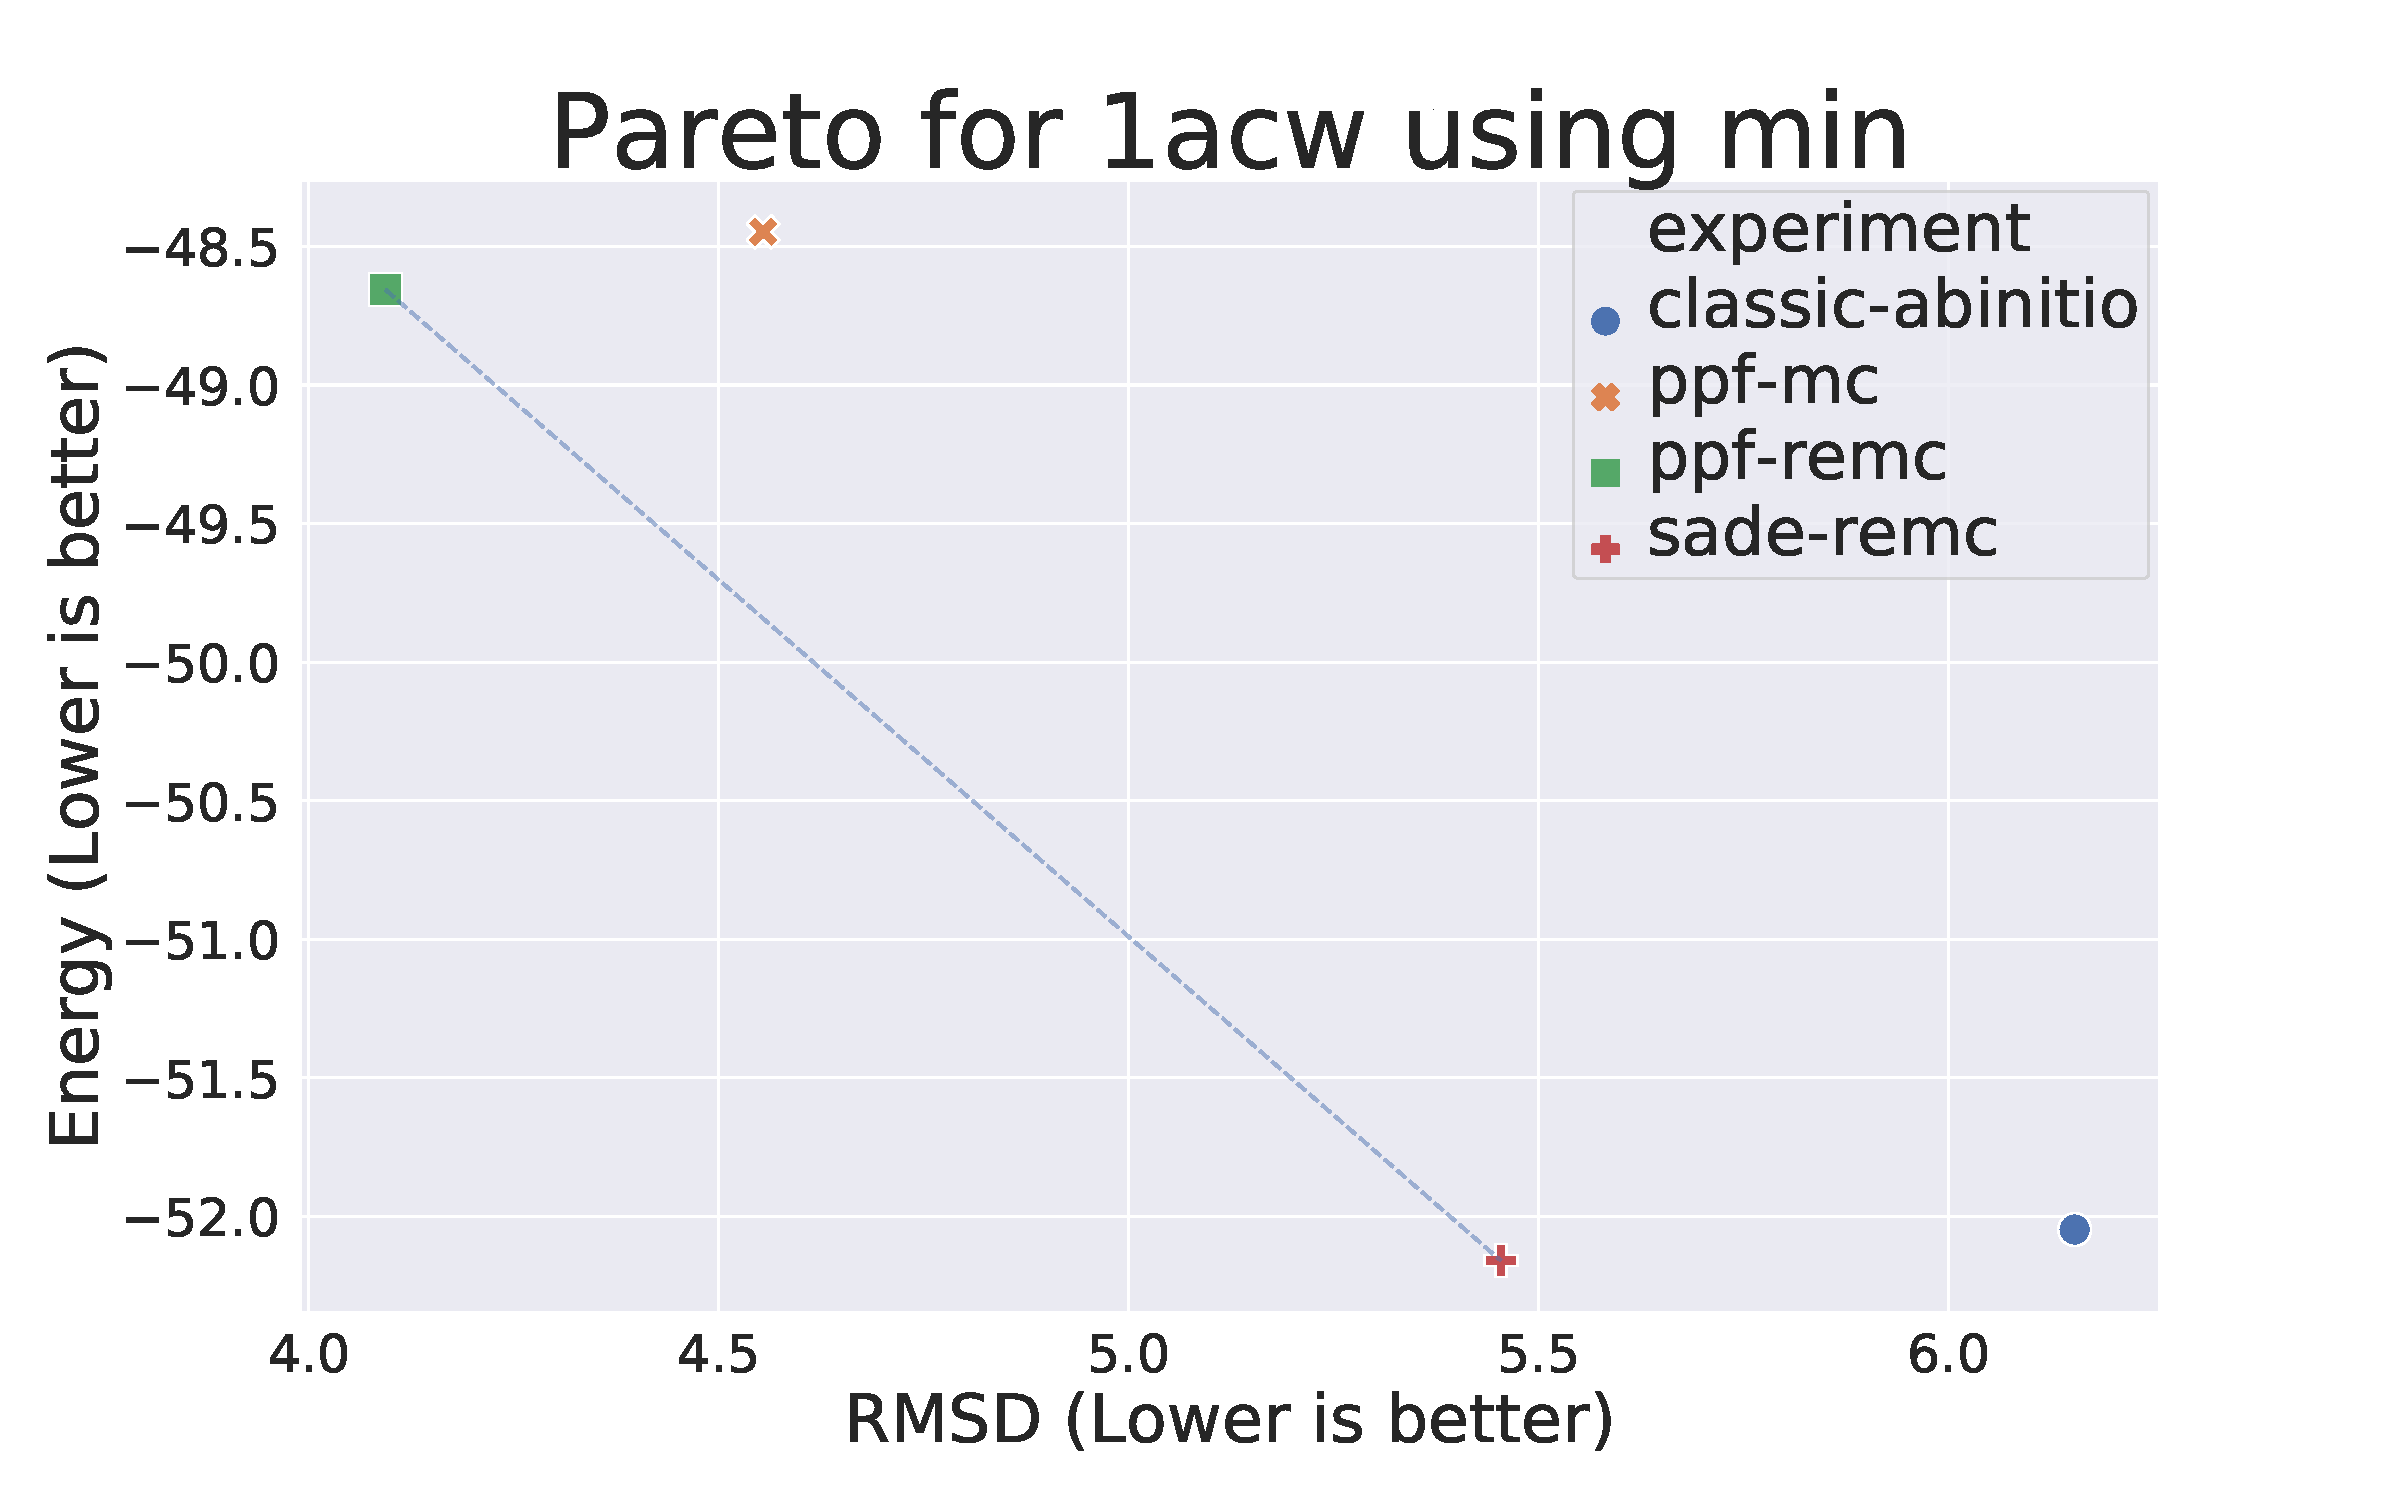
\includegraphics[width=1\linewidth]{Figuras/pareto/1acw_best_by_rmsd_min.pdf}
  \end{subfigure}
%
  \begin{subfigure}{0.49\linewidth}
    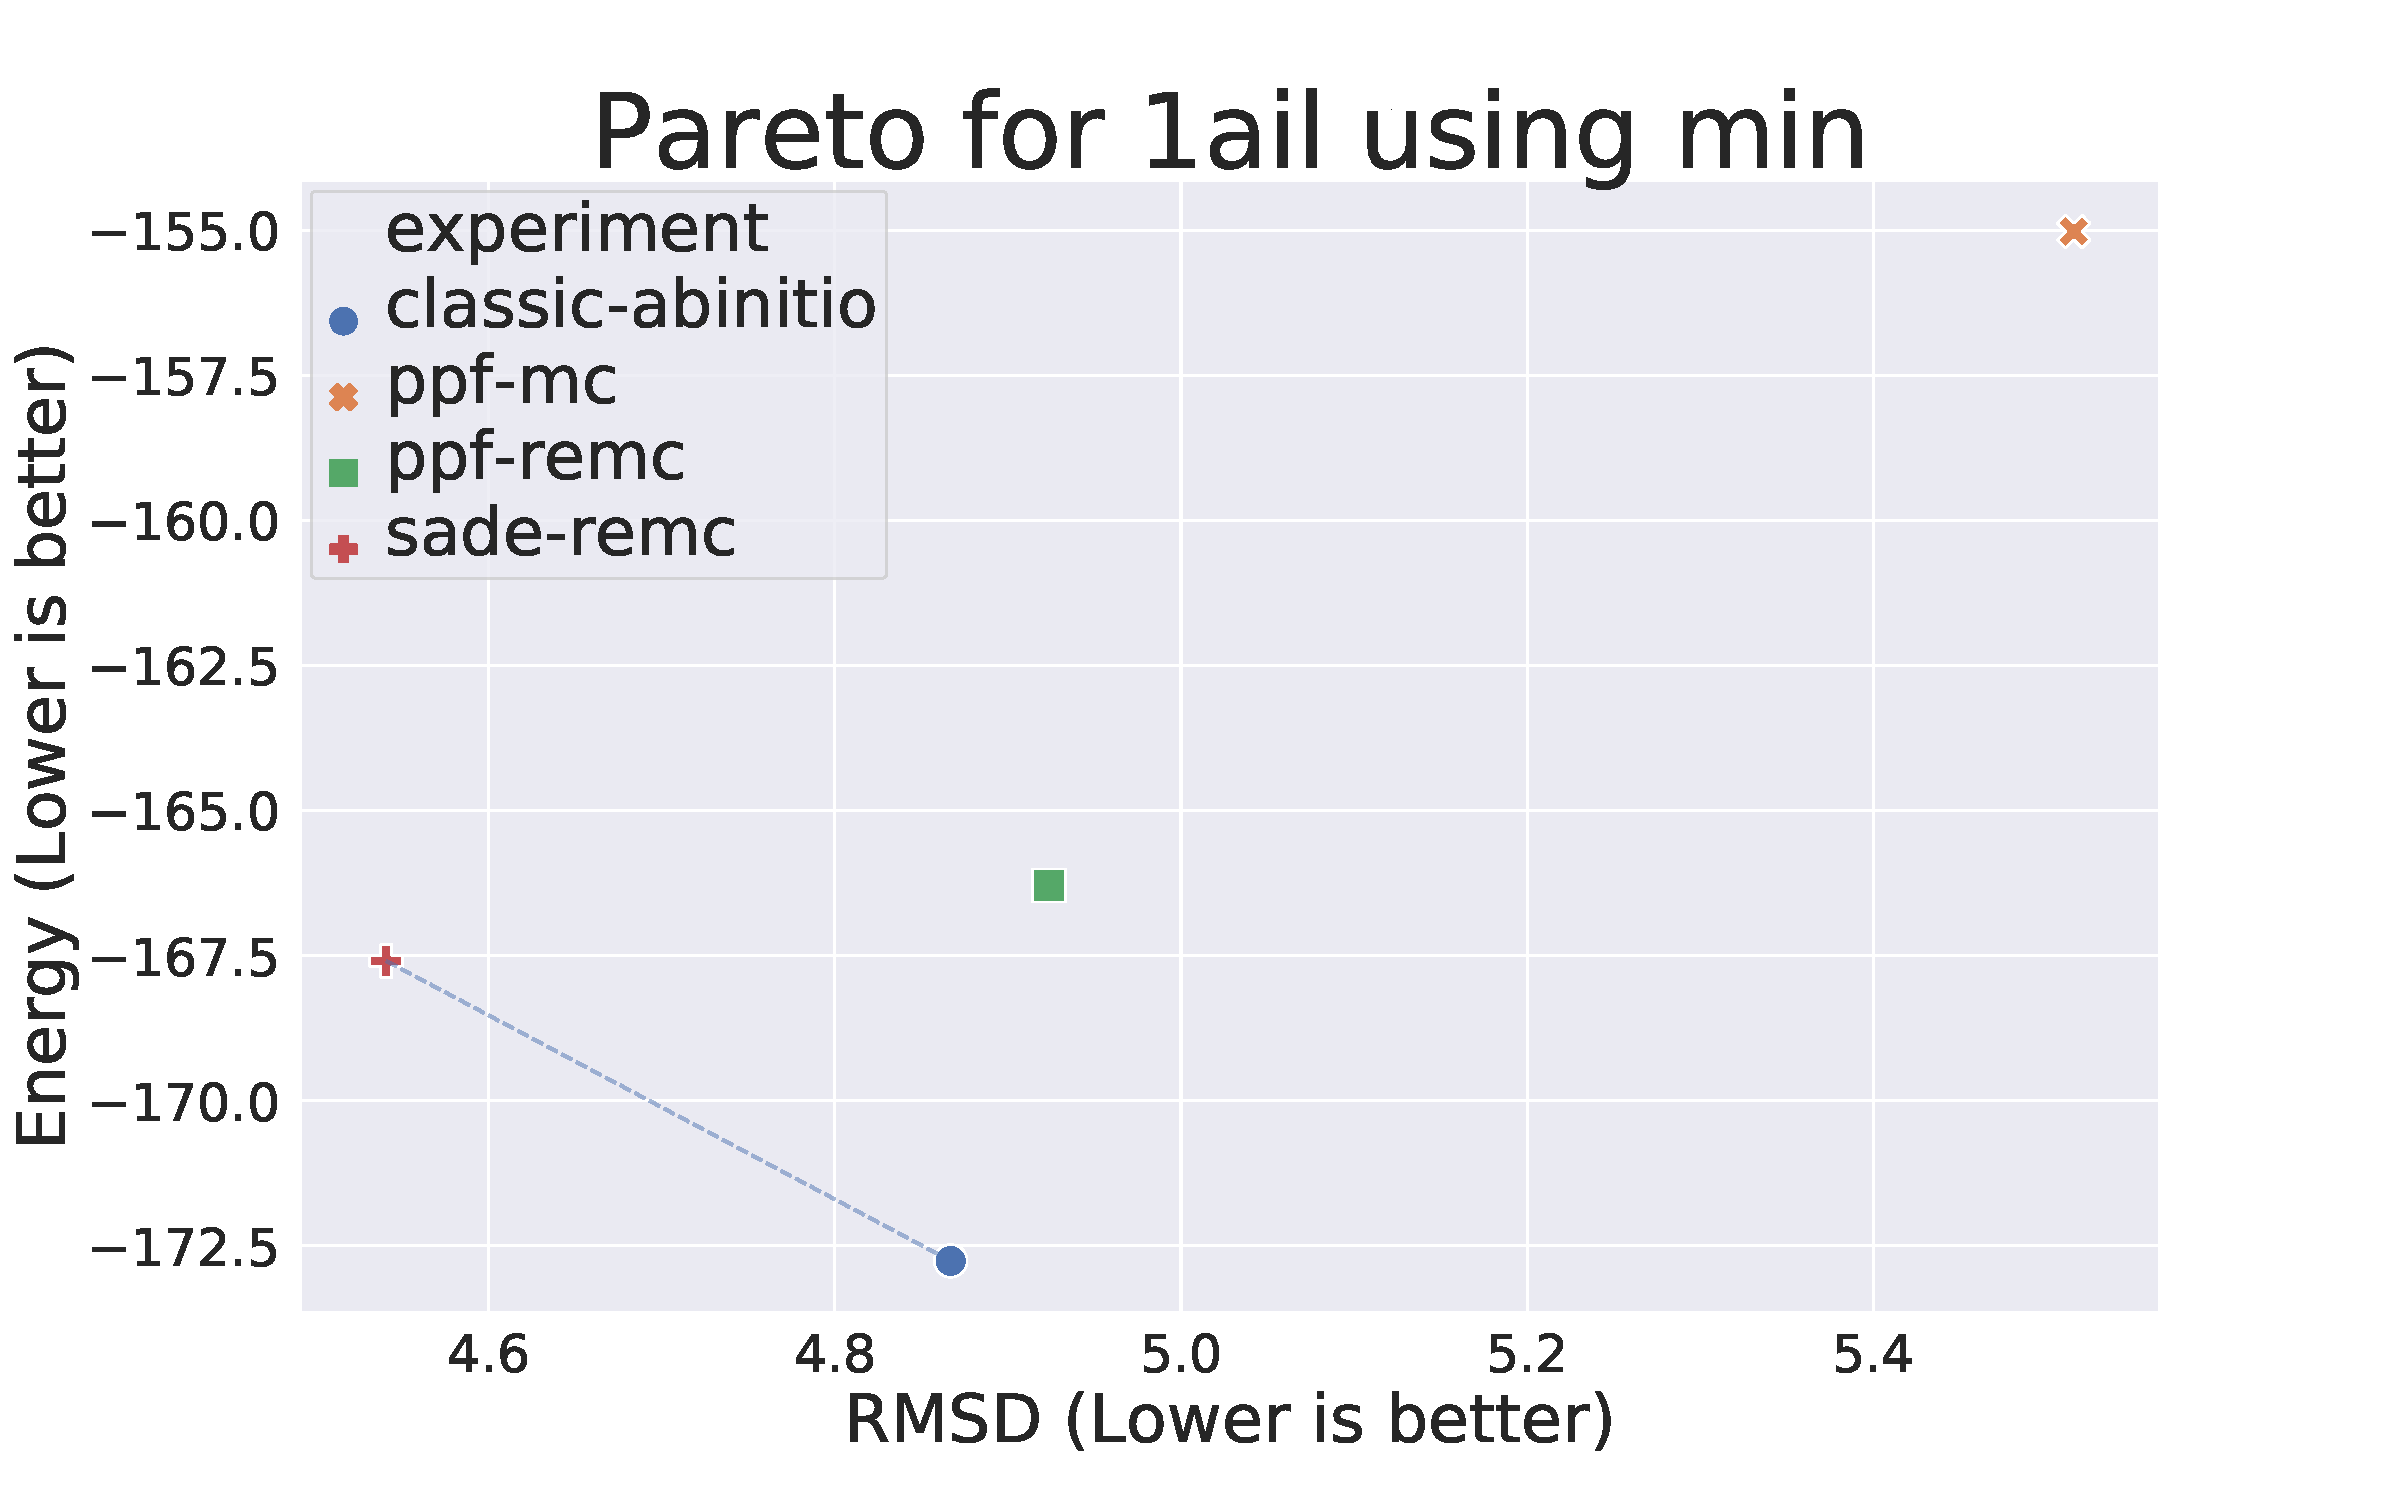
\includegraphics[width=1\linewidth]{Figuras/pareto/1ail_best_by_rmsd_min.pdf}
  \end{subfigure}
%
  \begin{subfigure}{0.49\linewidth}
    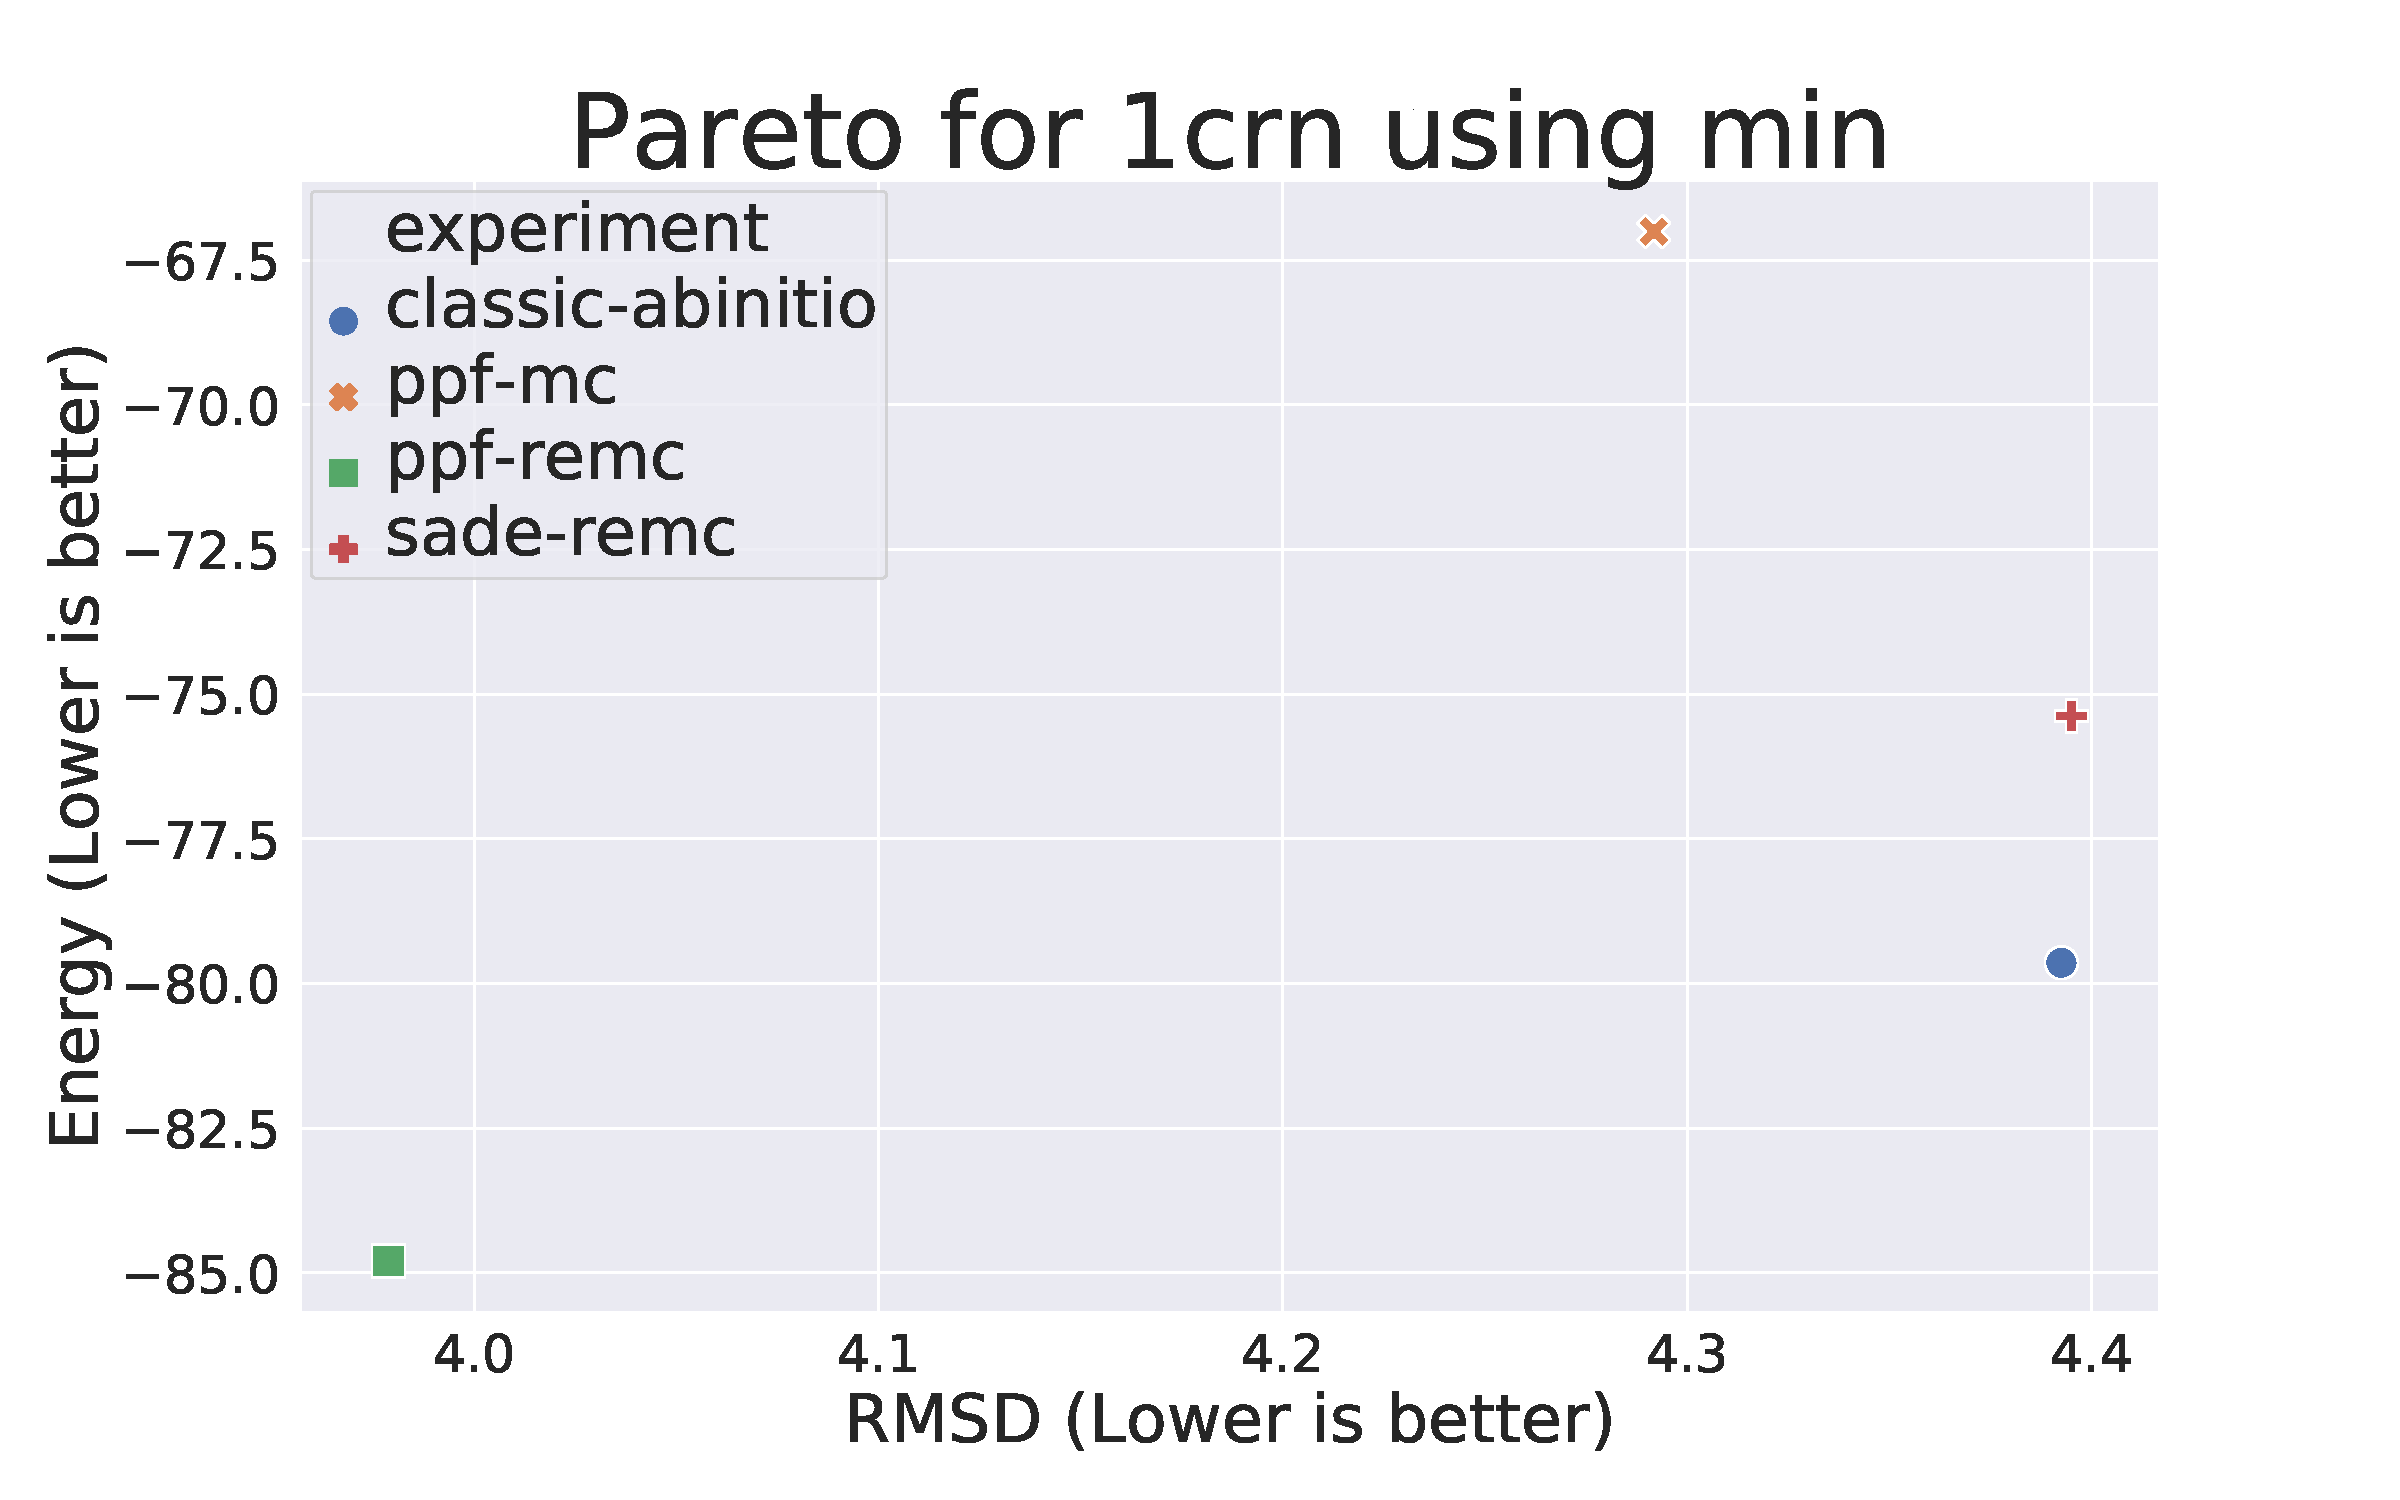
\includegraphics[width=1\linewidth]{Figuras/pareto/1crn_best_by_rmsd_min.pdf}
  \end{subfigure}
%
  \begin{subfigure}{0.49\linewidth}
    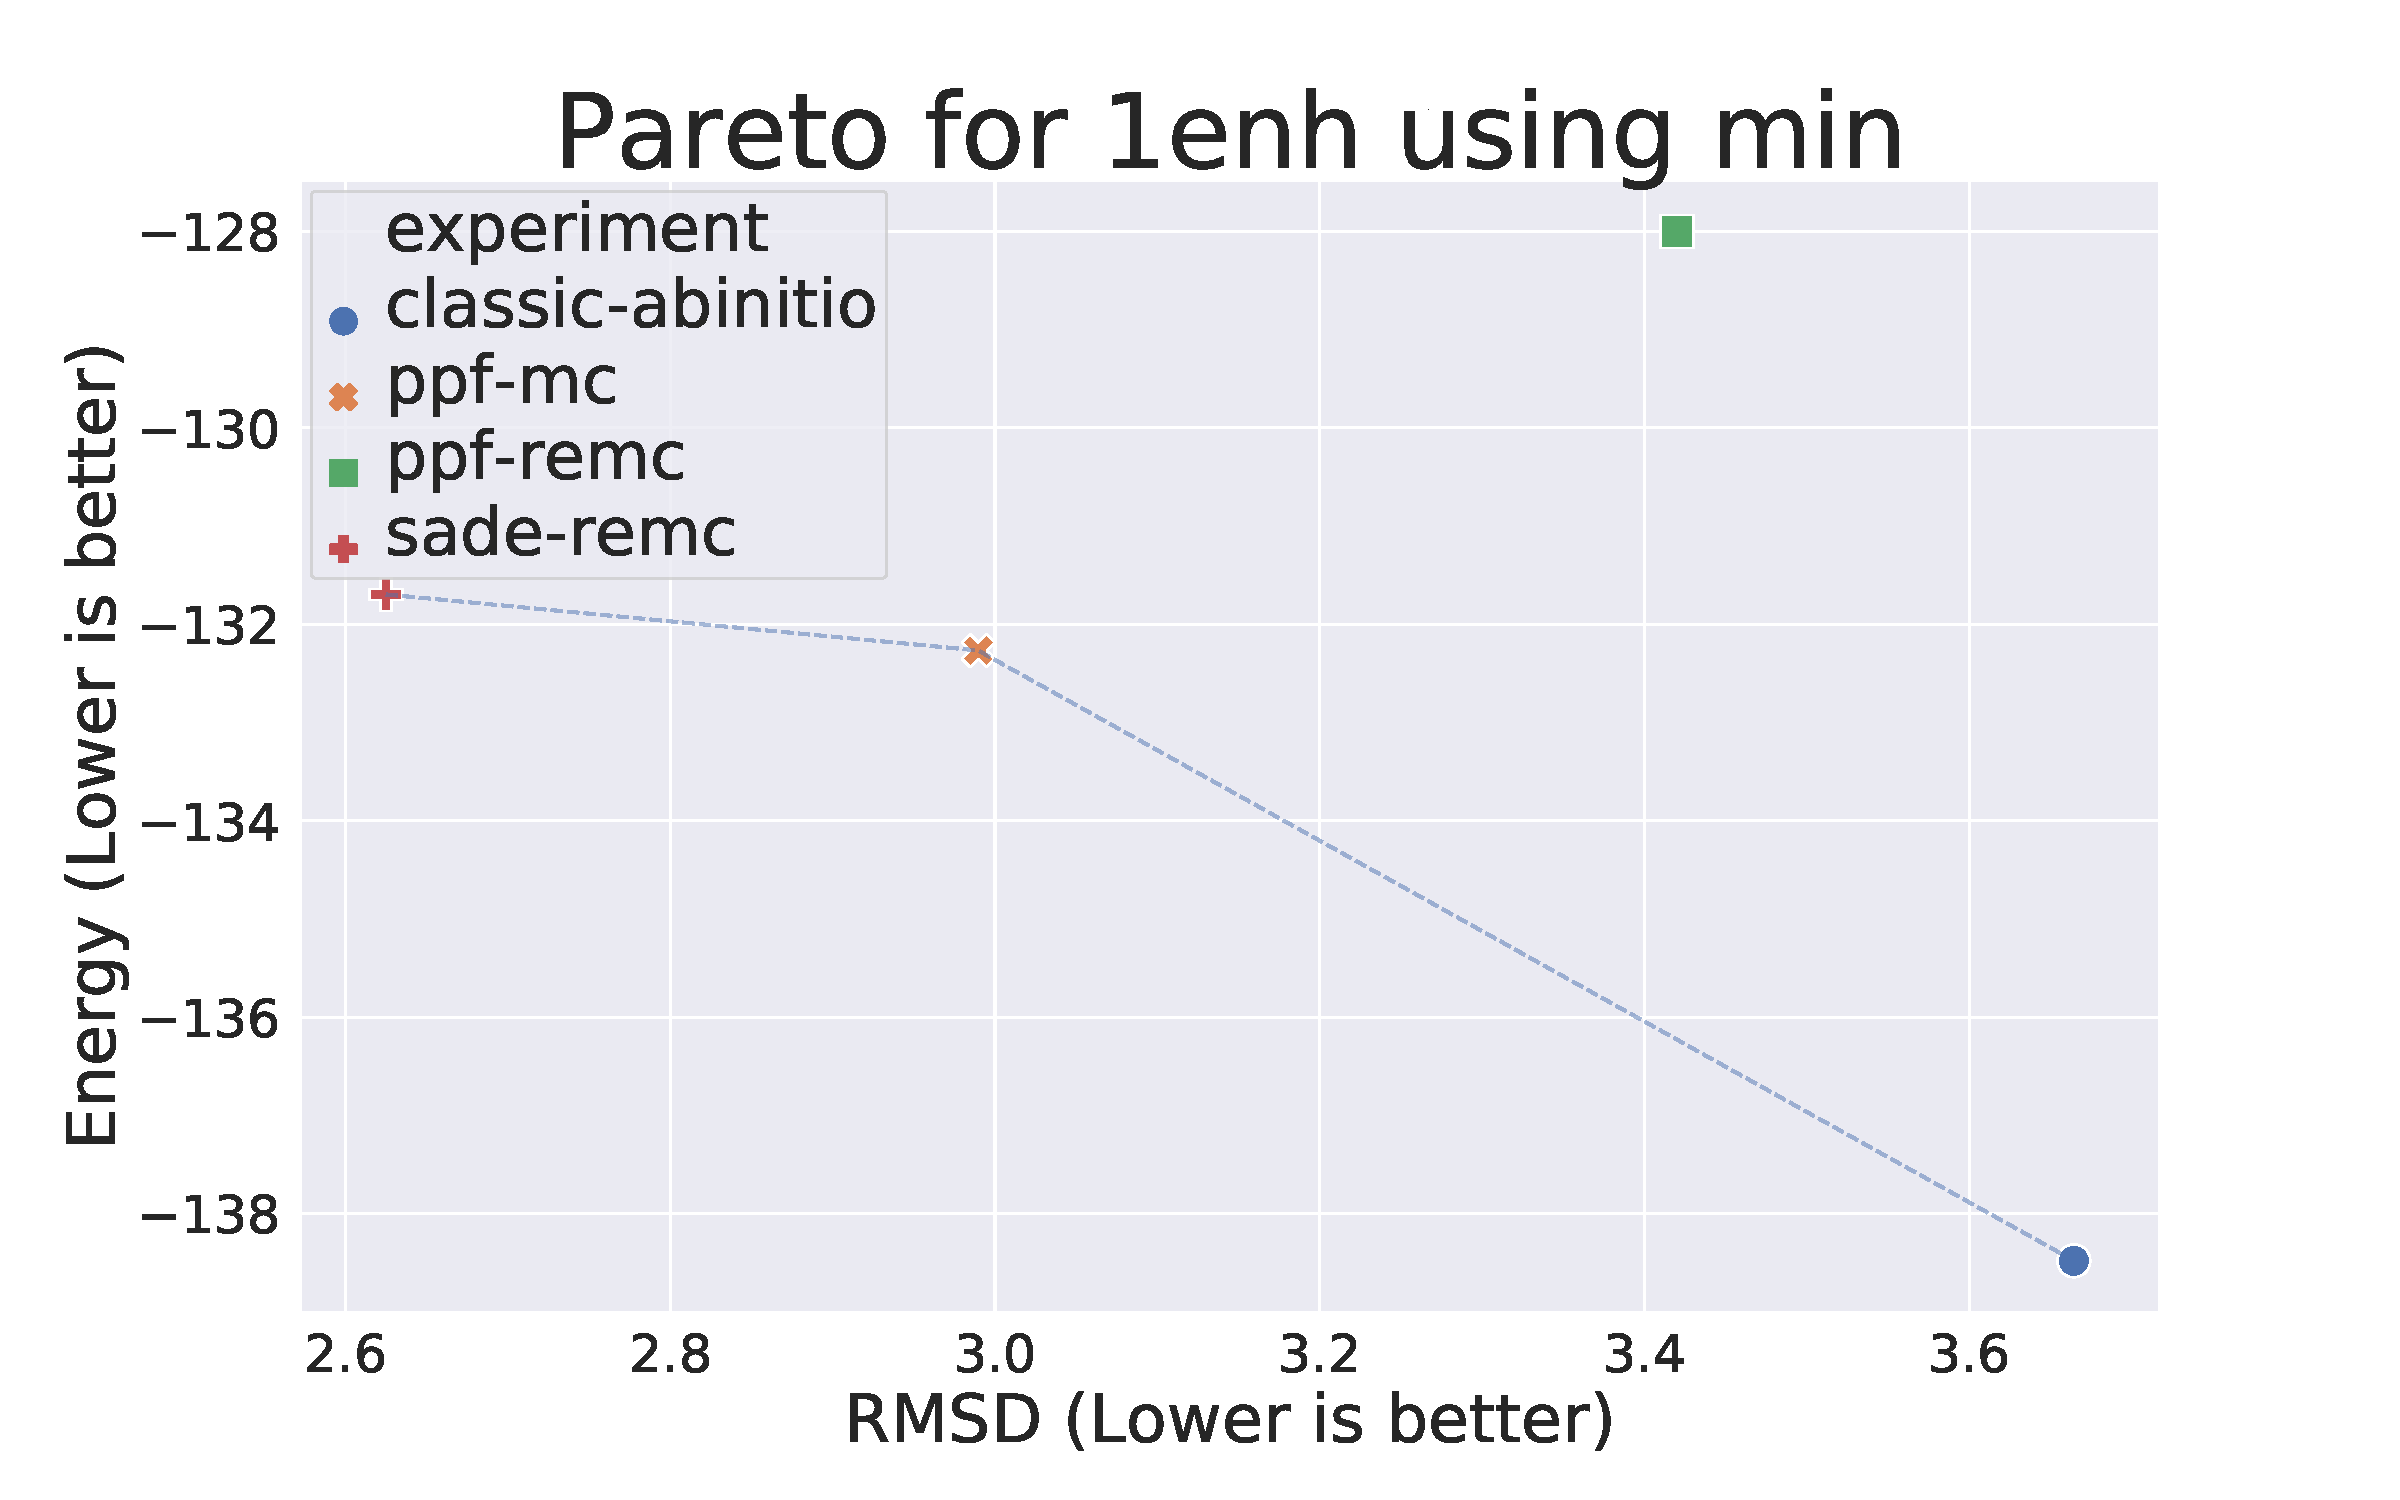
\includegraphics[width=1\linewidth]{Figuras/pareto/1enh_best_by_rmsd_min.pdf}
  \end{subfigure}
%
  \begin{subfigure}{0.49\linewidth}
    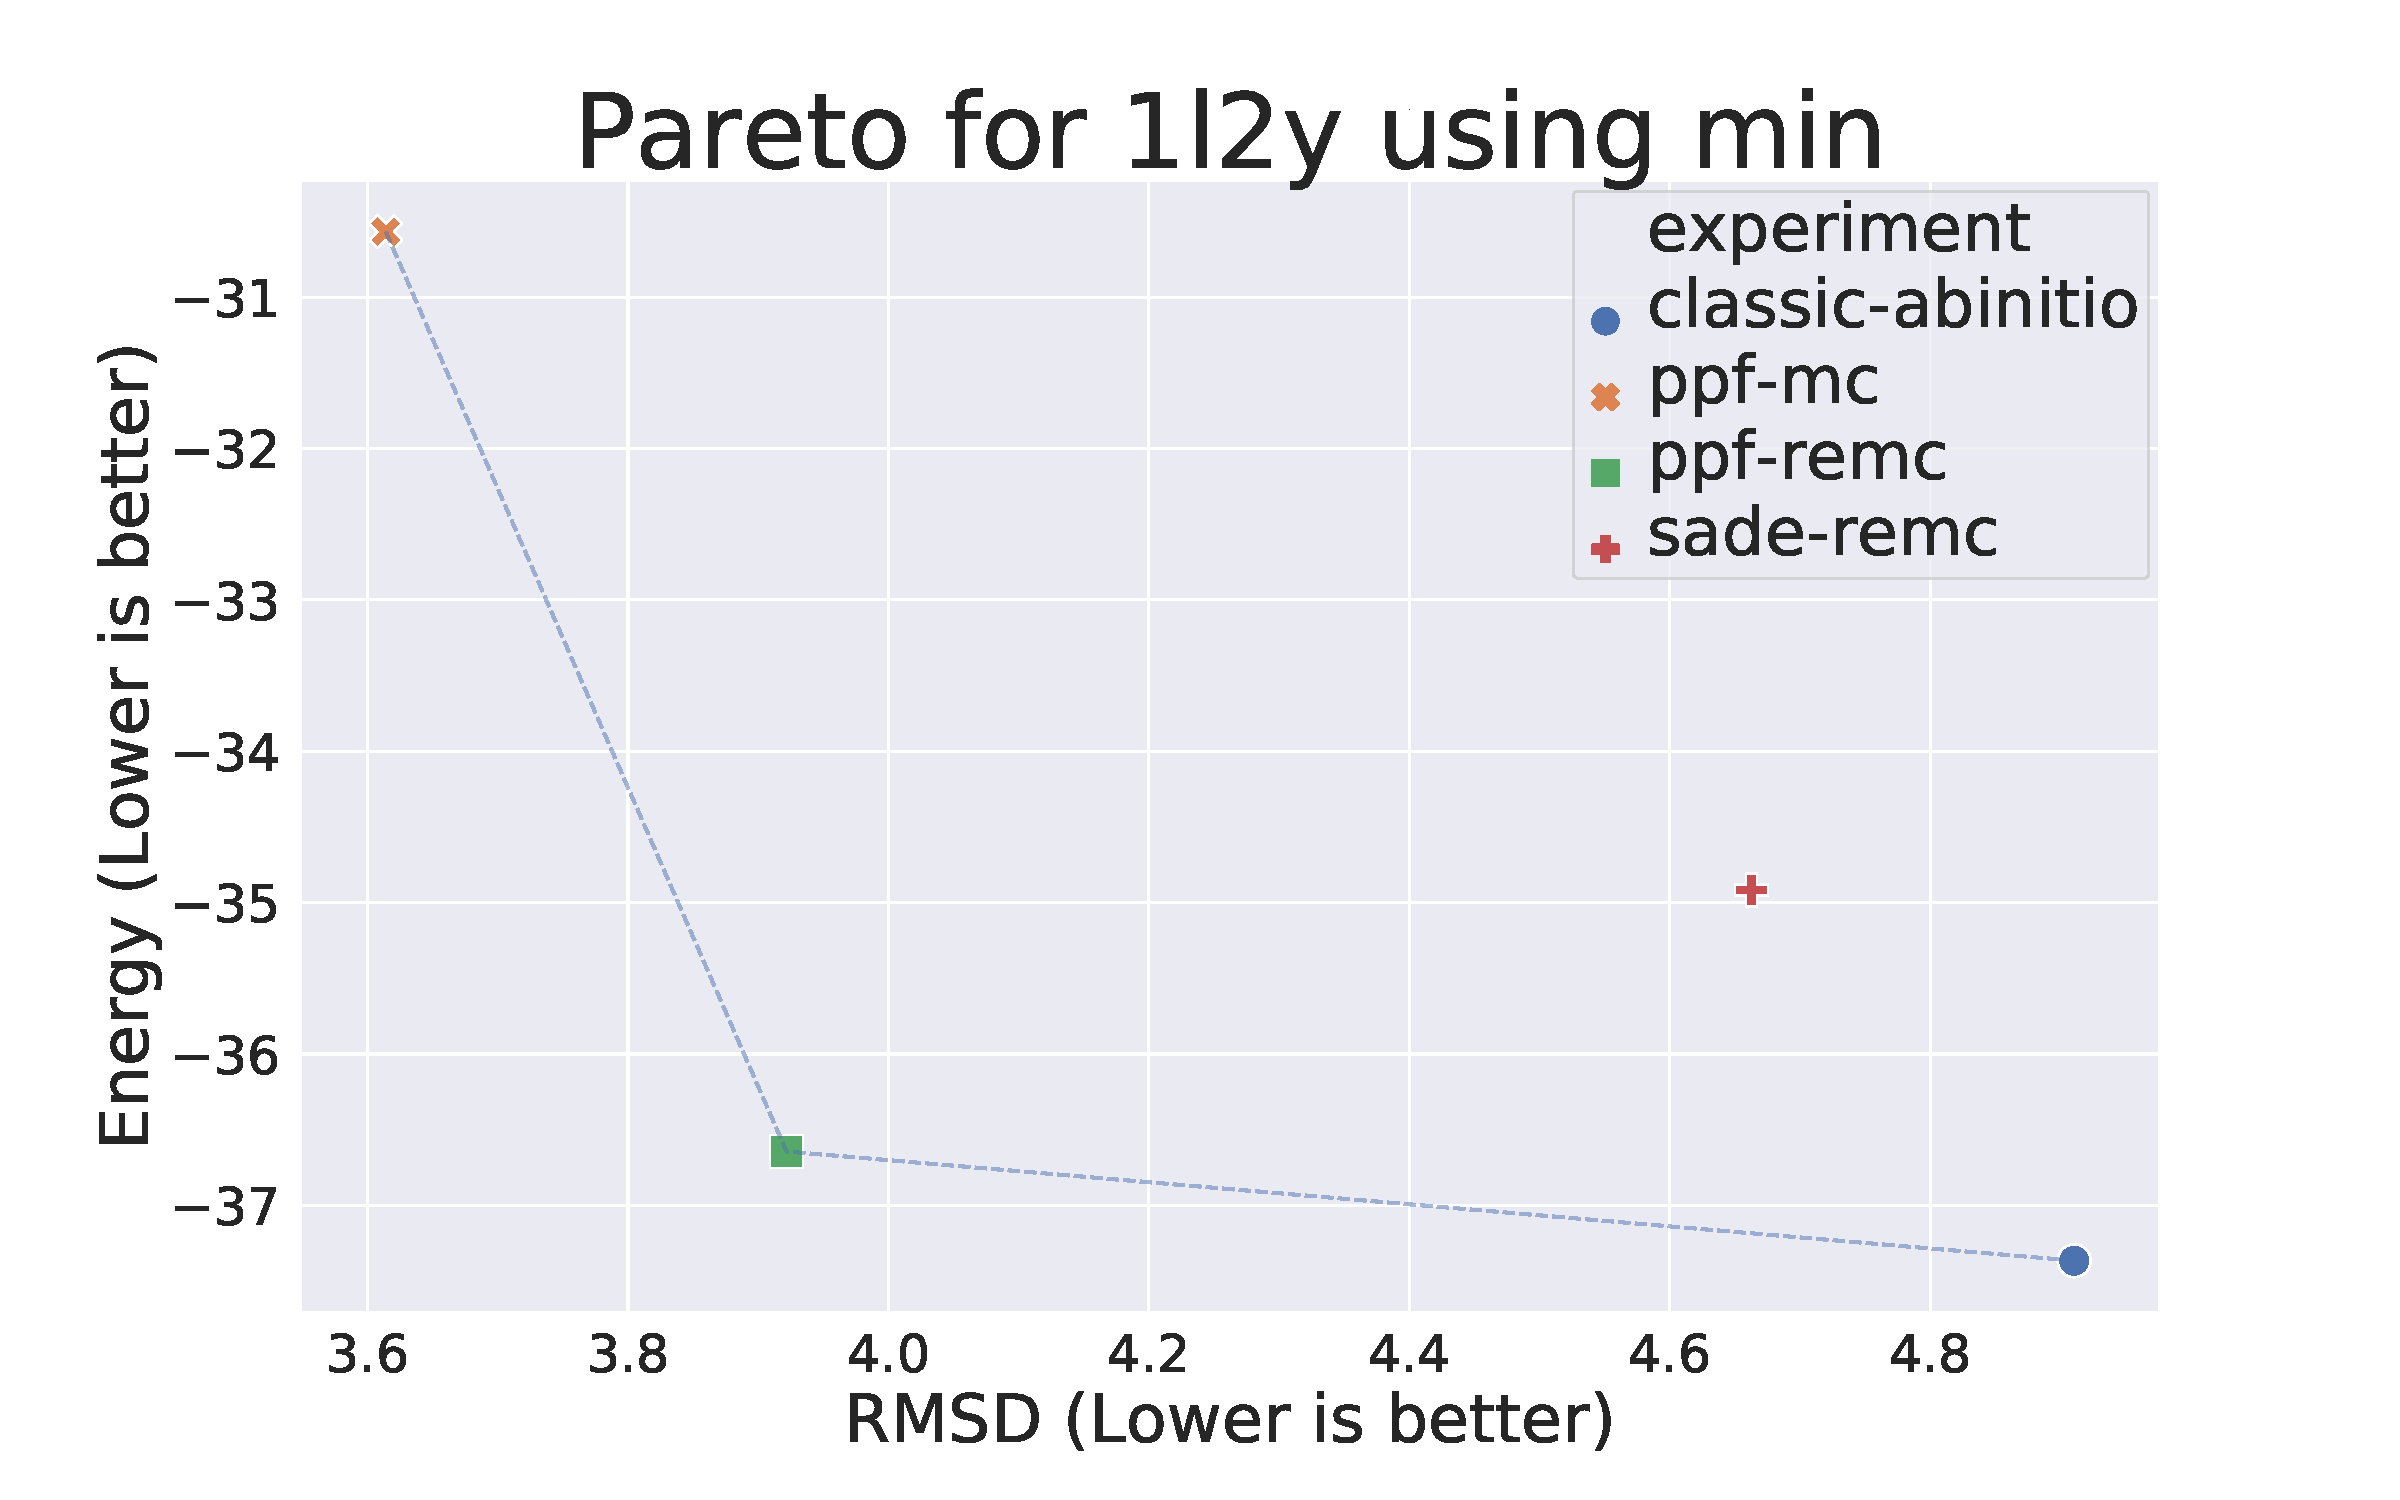
\includegraphics[width=1\linewidth]{Figuras/pareto/1l2y_best_by_rmsd_min.pdf}
  \end{subfigure}
%
  \begin{subfigure}{0.49\linewidth}
    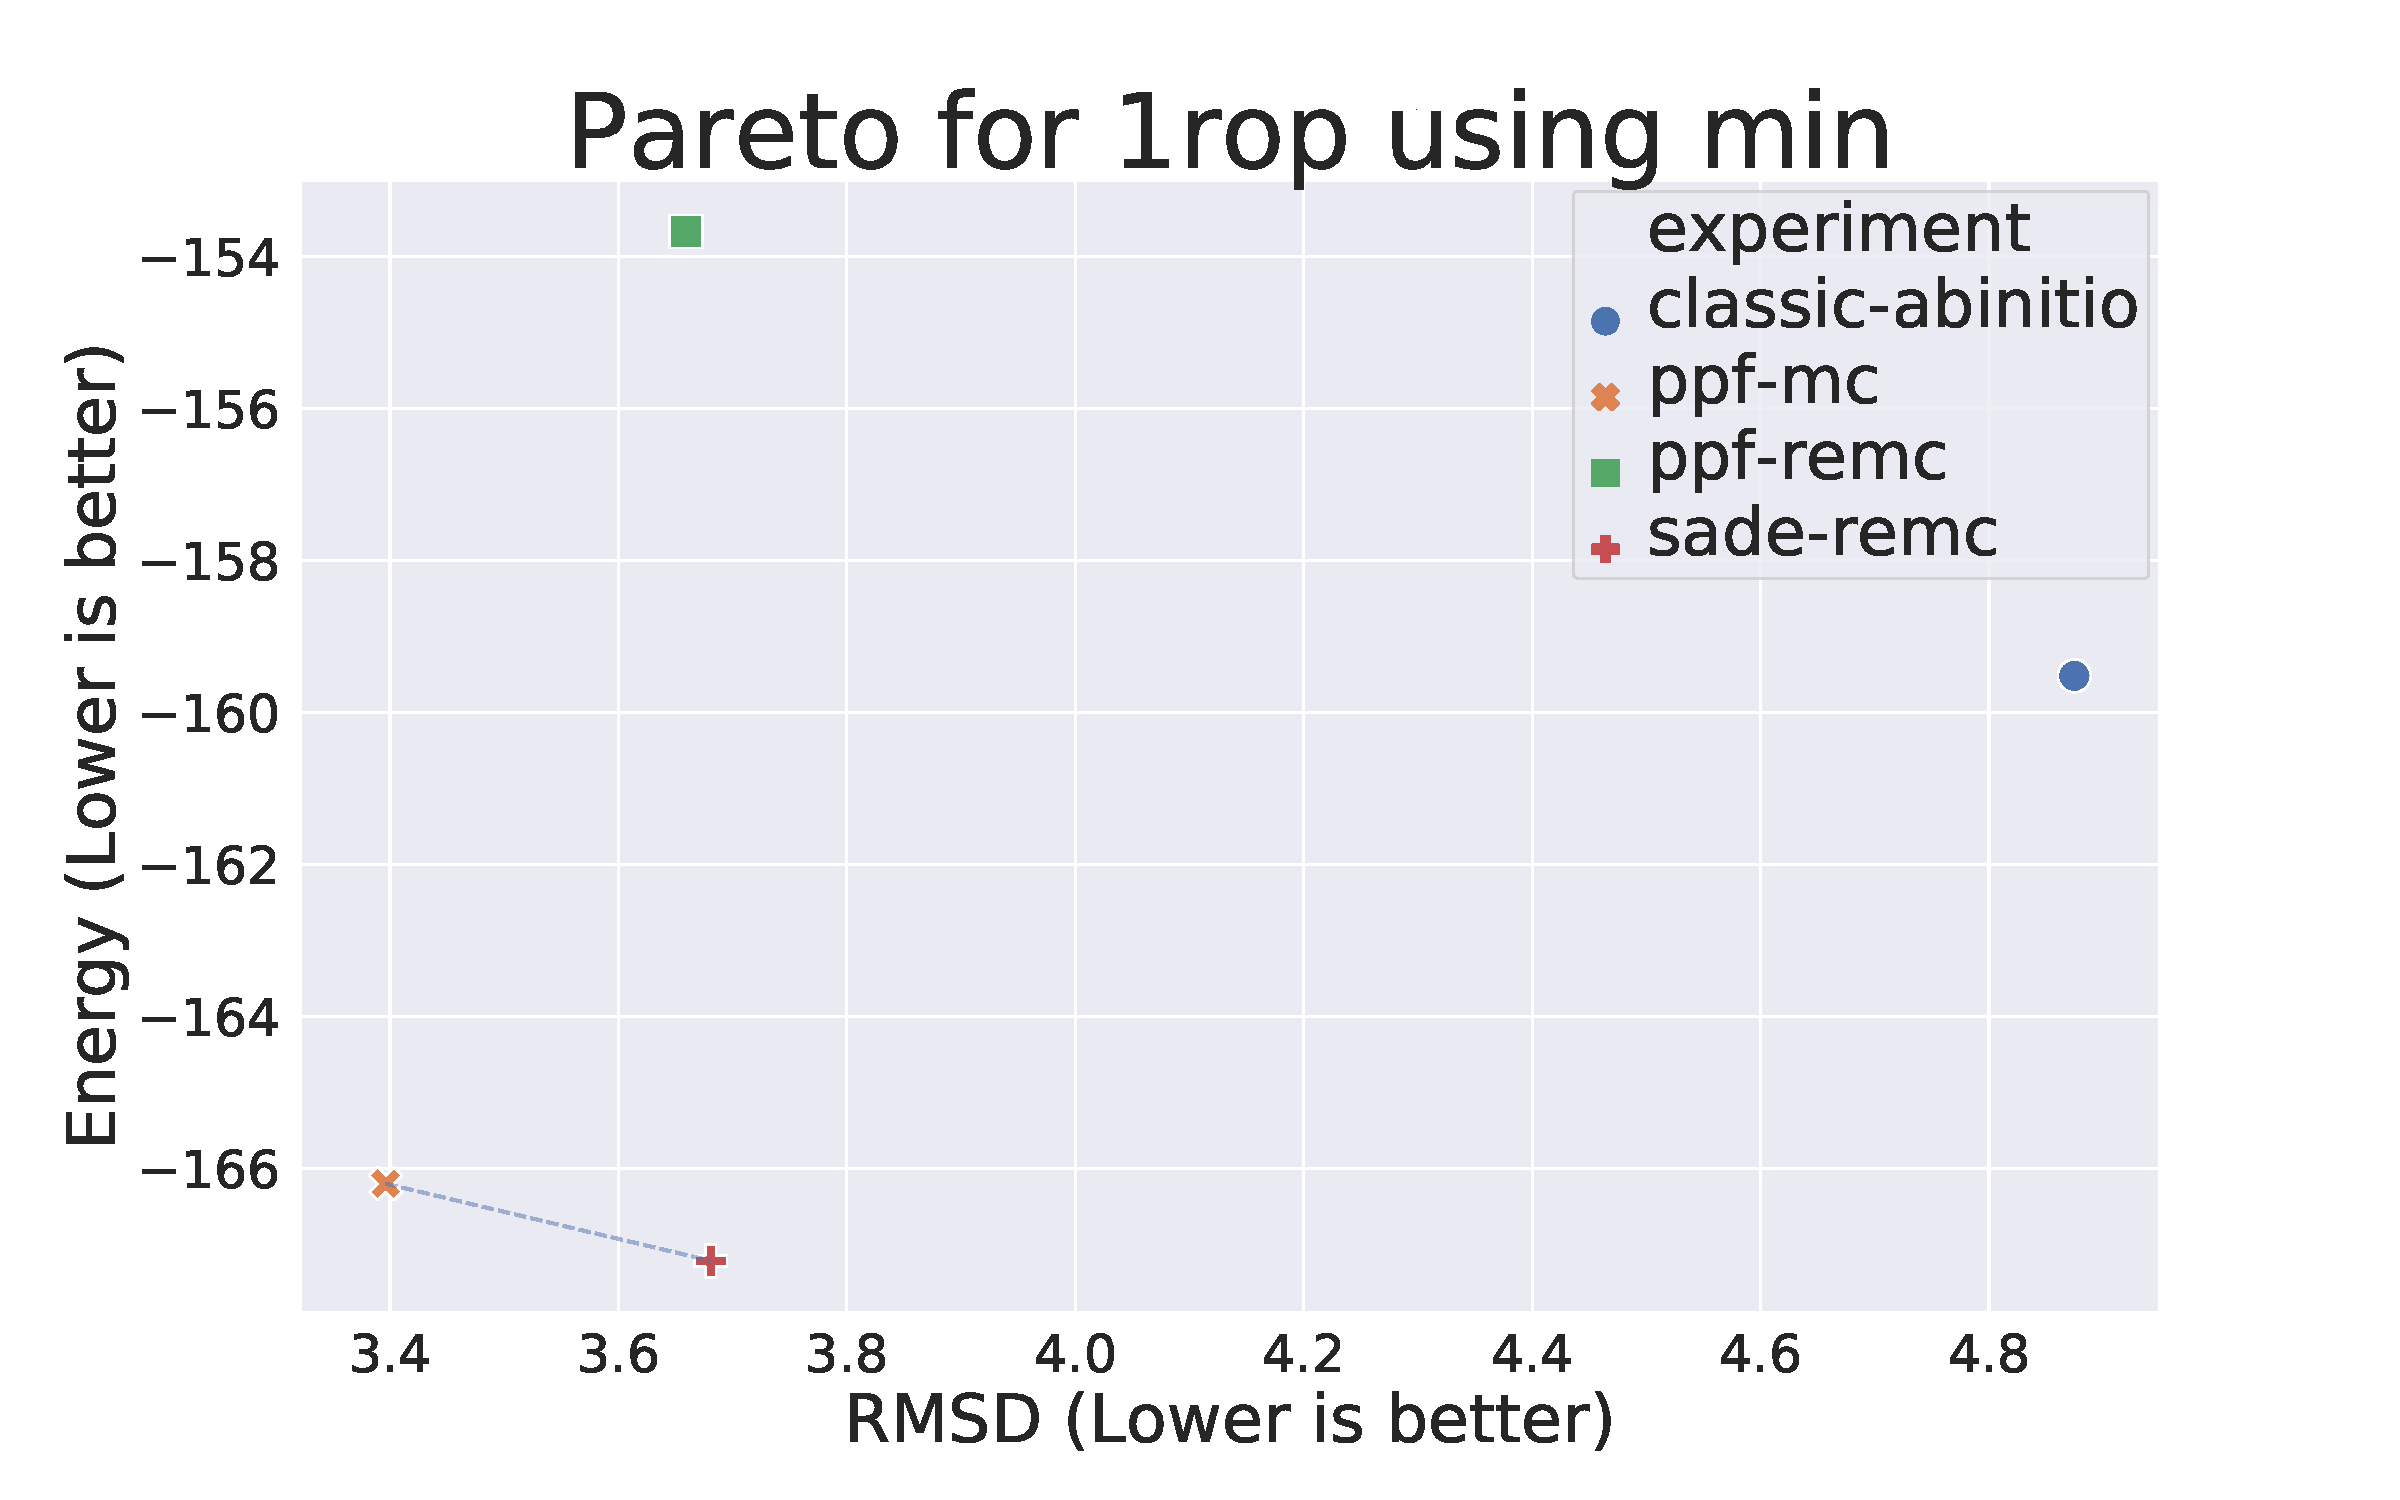
\includegraphics[width=1\linewidth]{Figuras/pareto/1rop_best_by_rmsd_min.pdf}
  \end{subfigure}
%
  \begin{subfigure}{0.49\linewidth}
    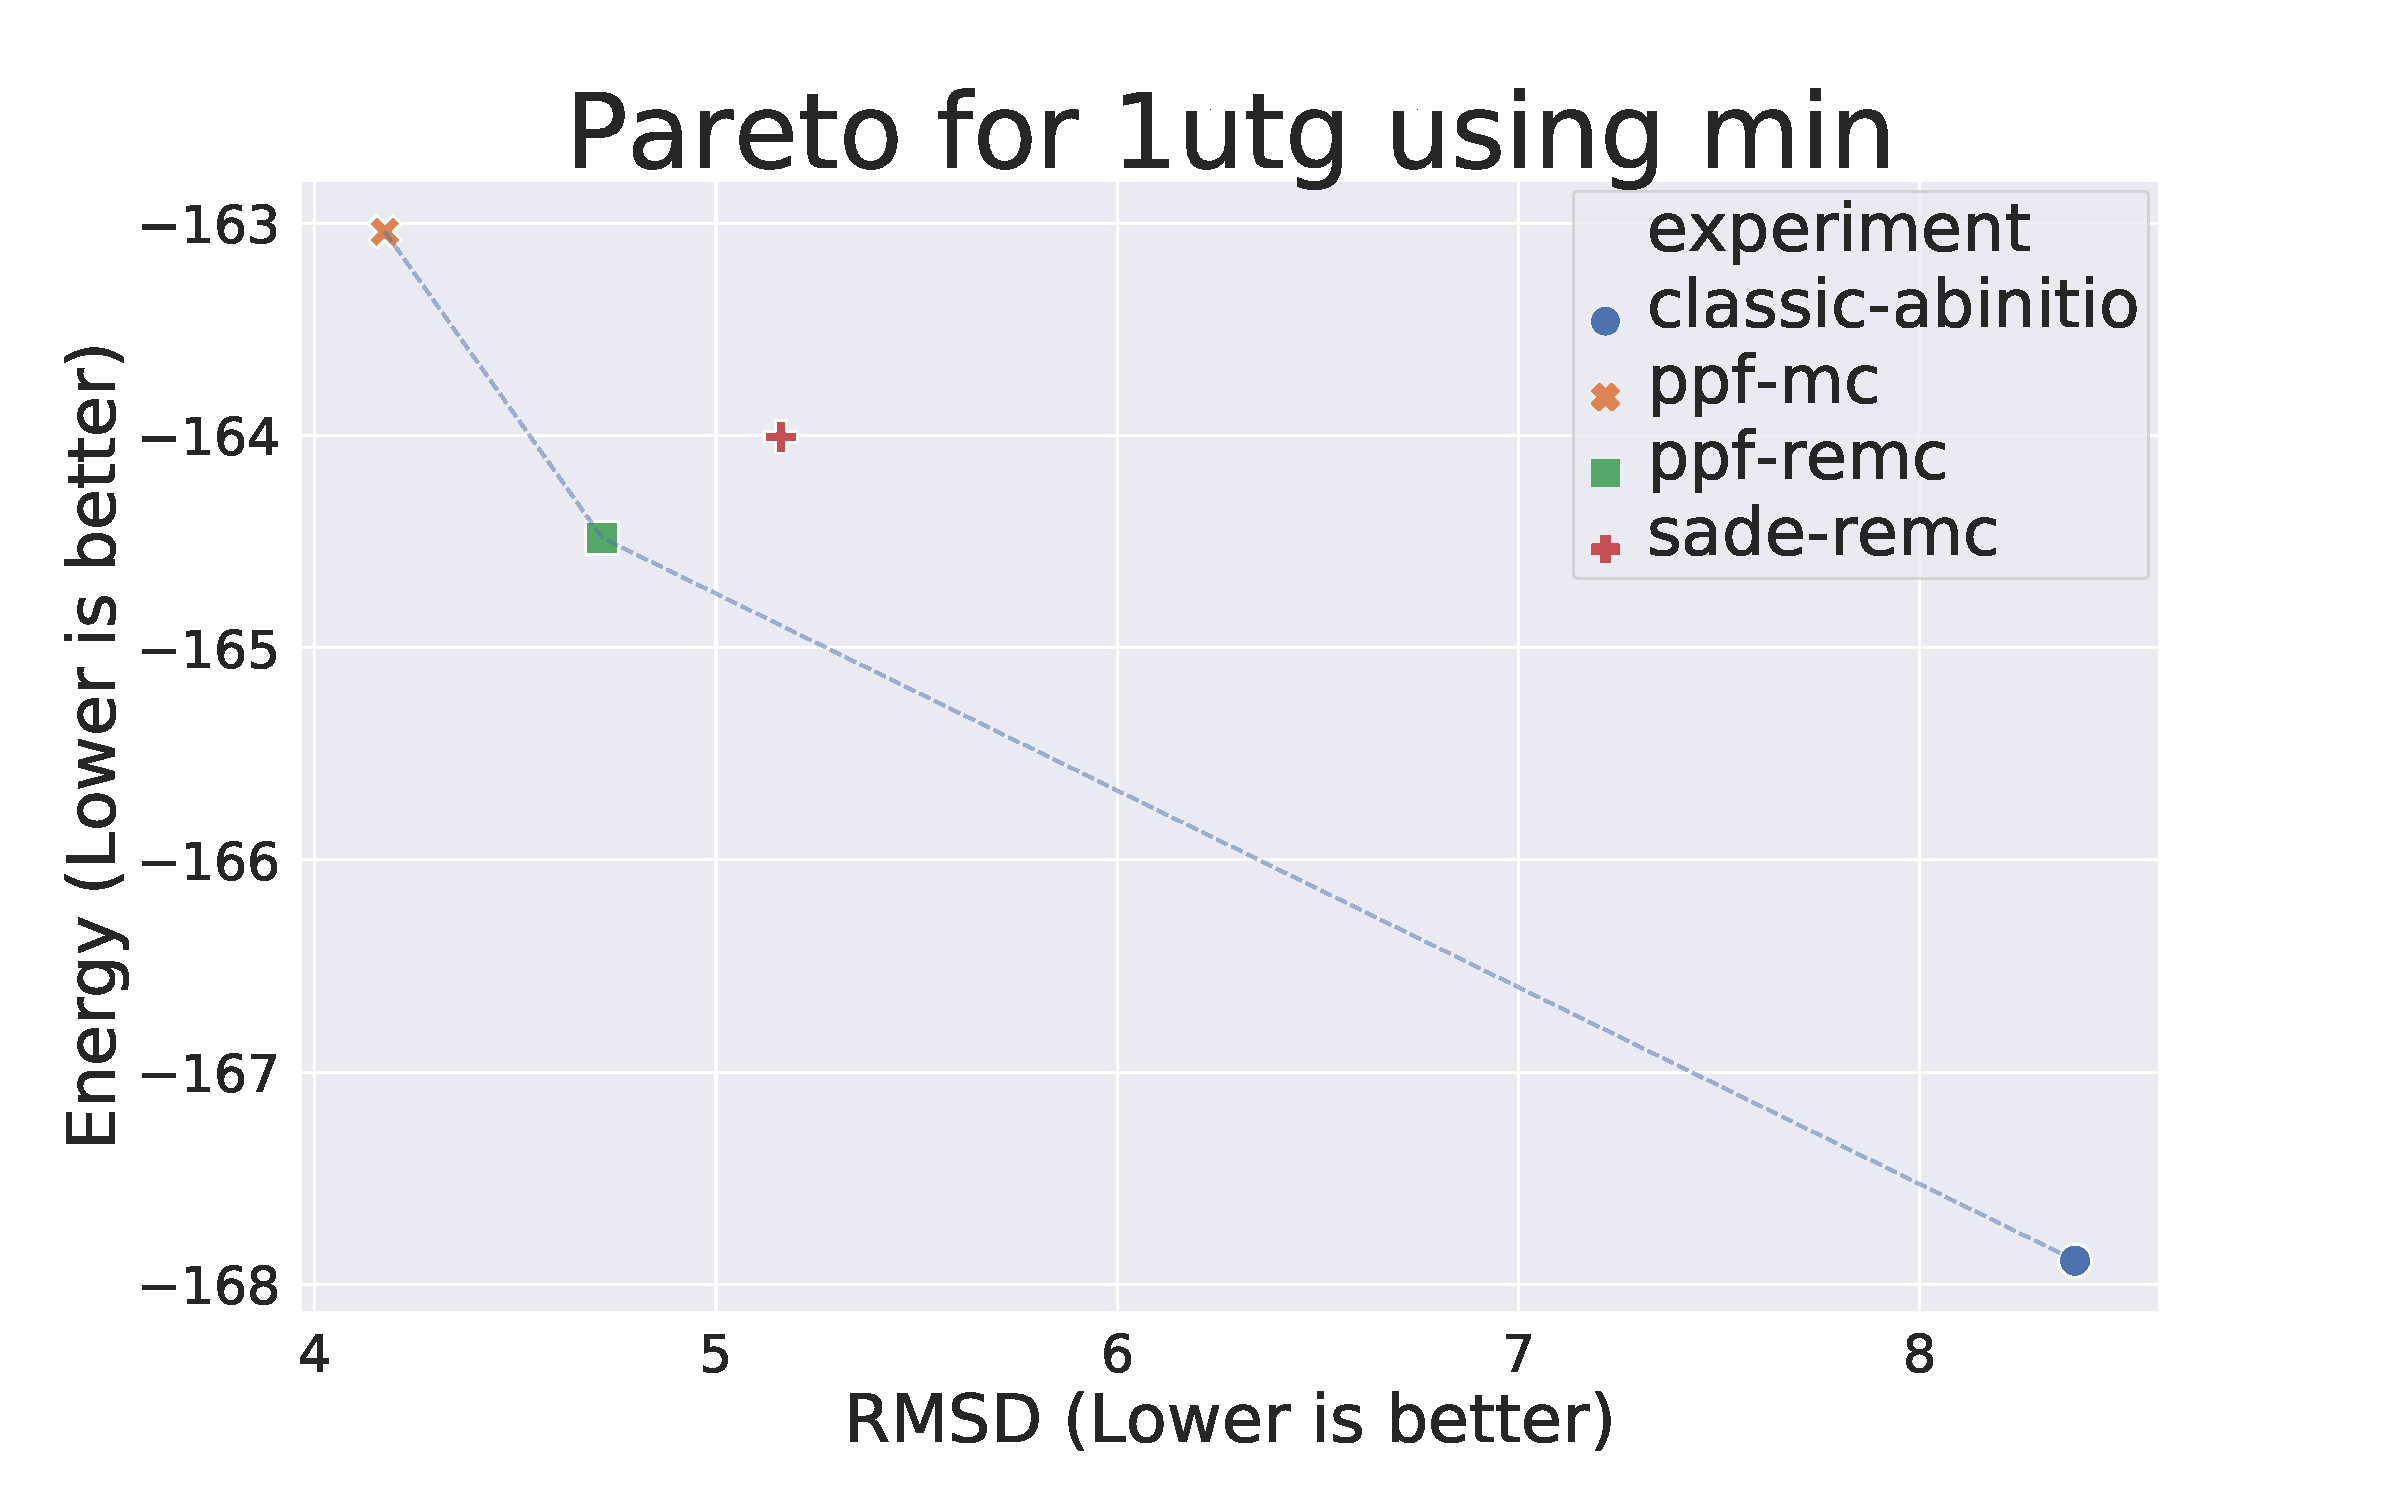
\includegraphics[width=1\linewidth]{Figuras/pareto/1utg_best_by_rmsd_min.pdf}
  \end{subfigure}
%
  \begin{subfigure}{0.49\linewidth}
    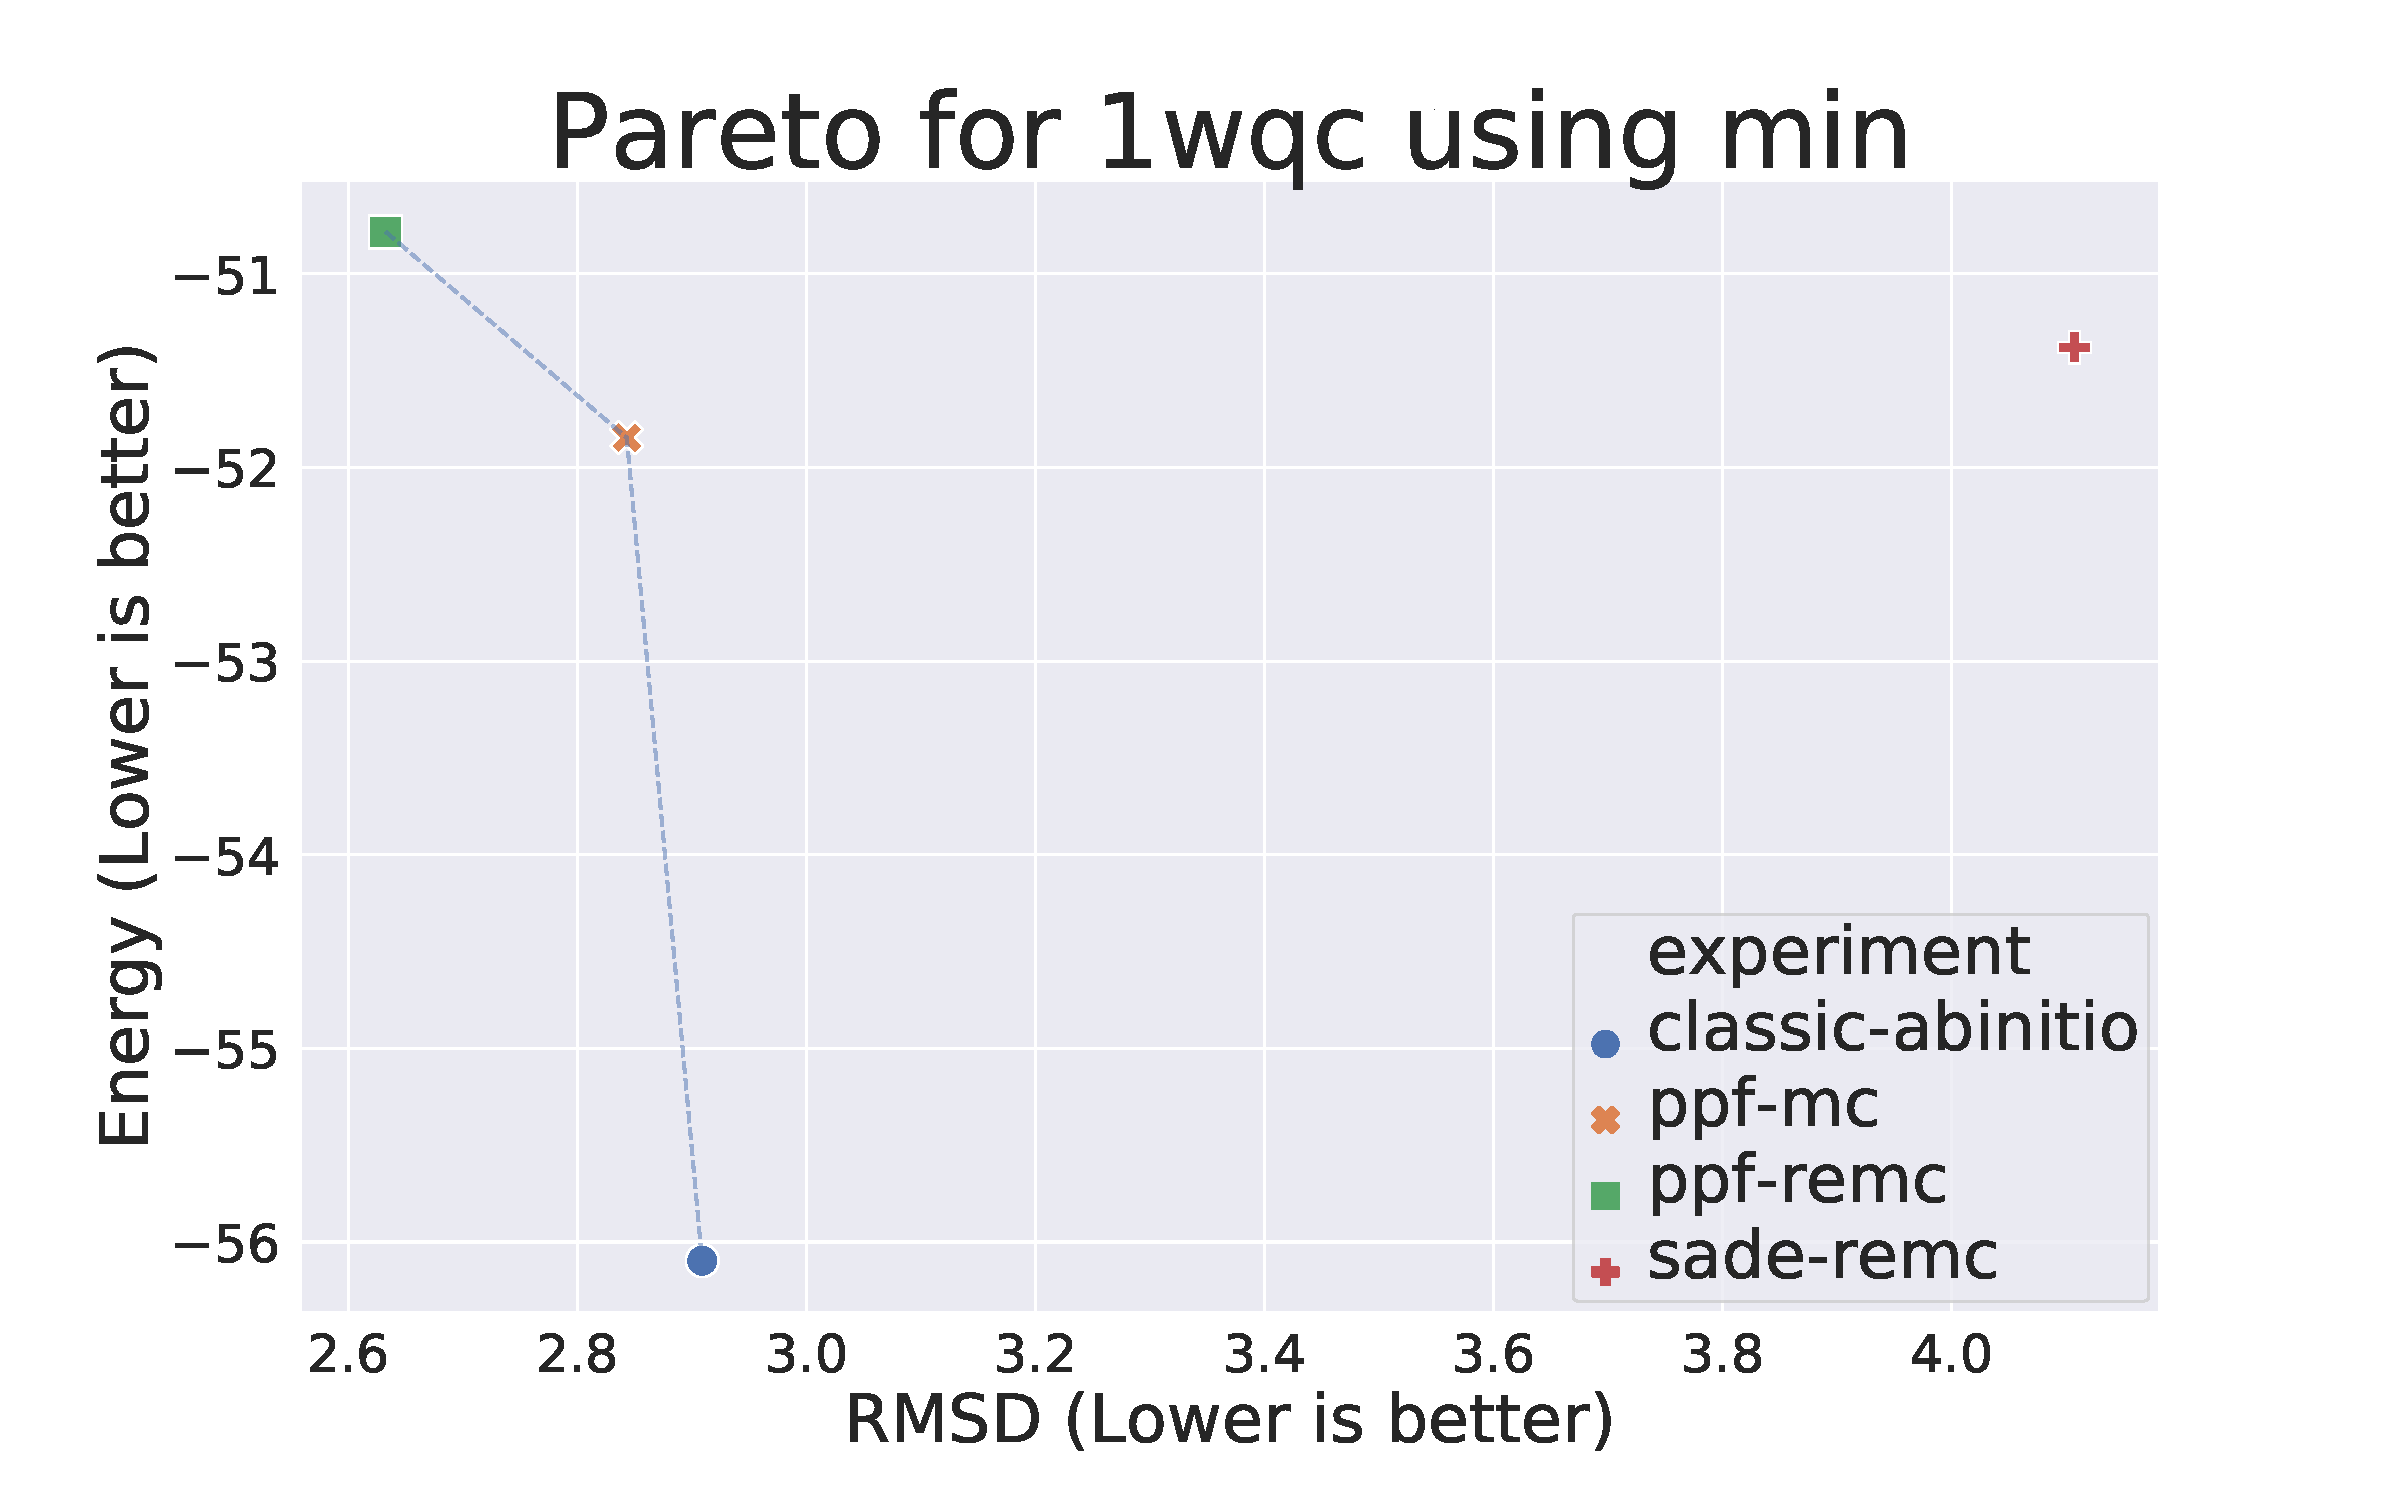
\includegraphics[width=1\linewidth]{Figuras/pareto/1wqc_best_by_rmsd_min.pdf}
  \end{subfigure}
%
  \begin{subfigure}{0.49\linewidth}
    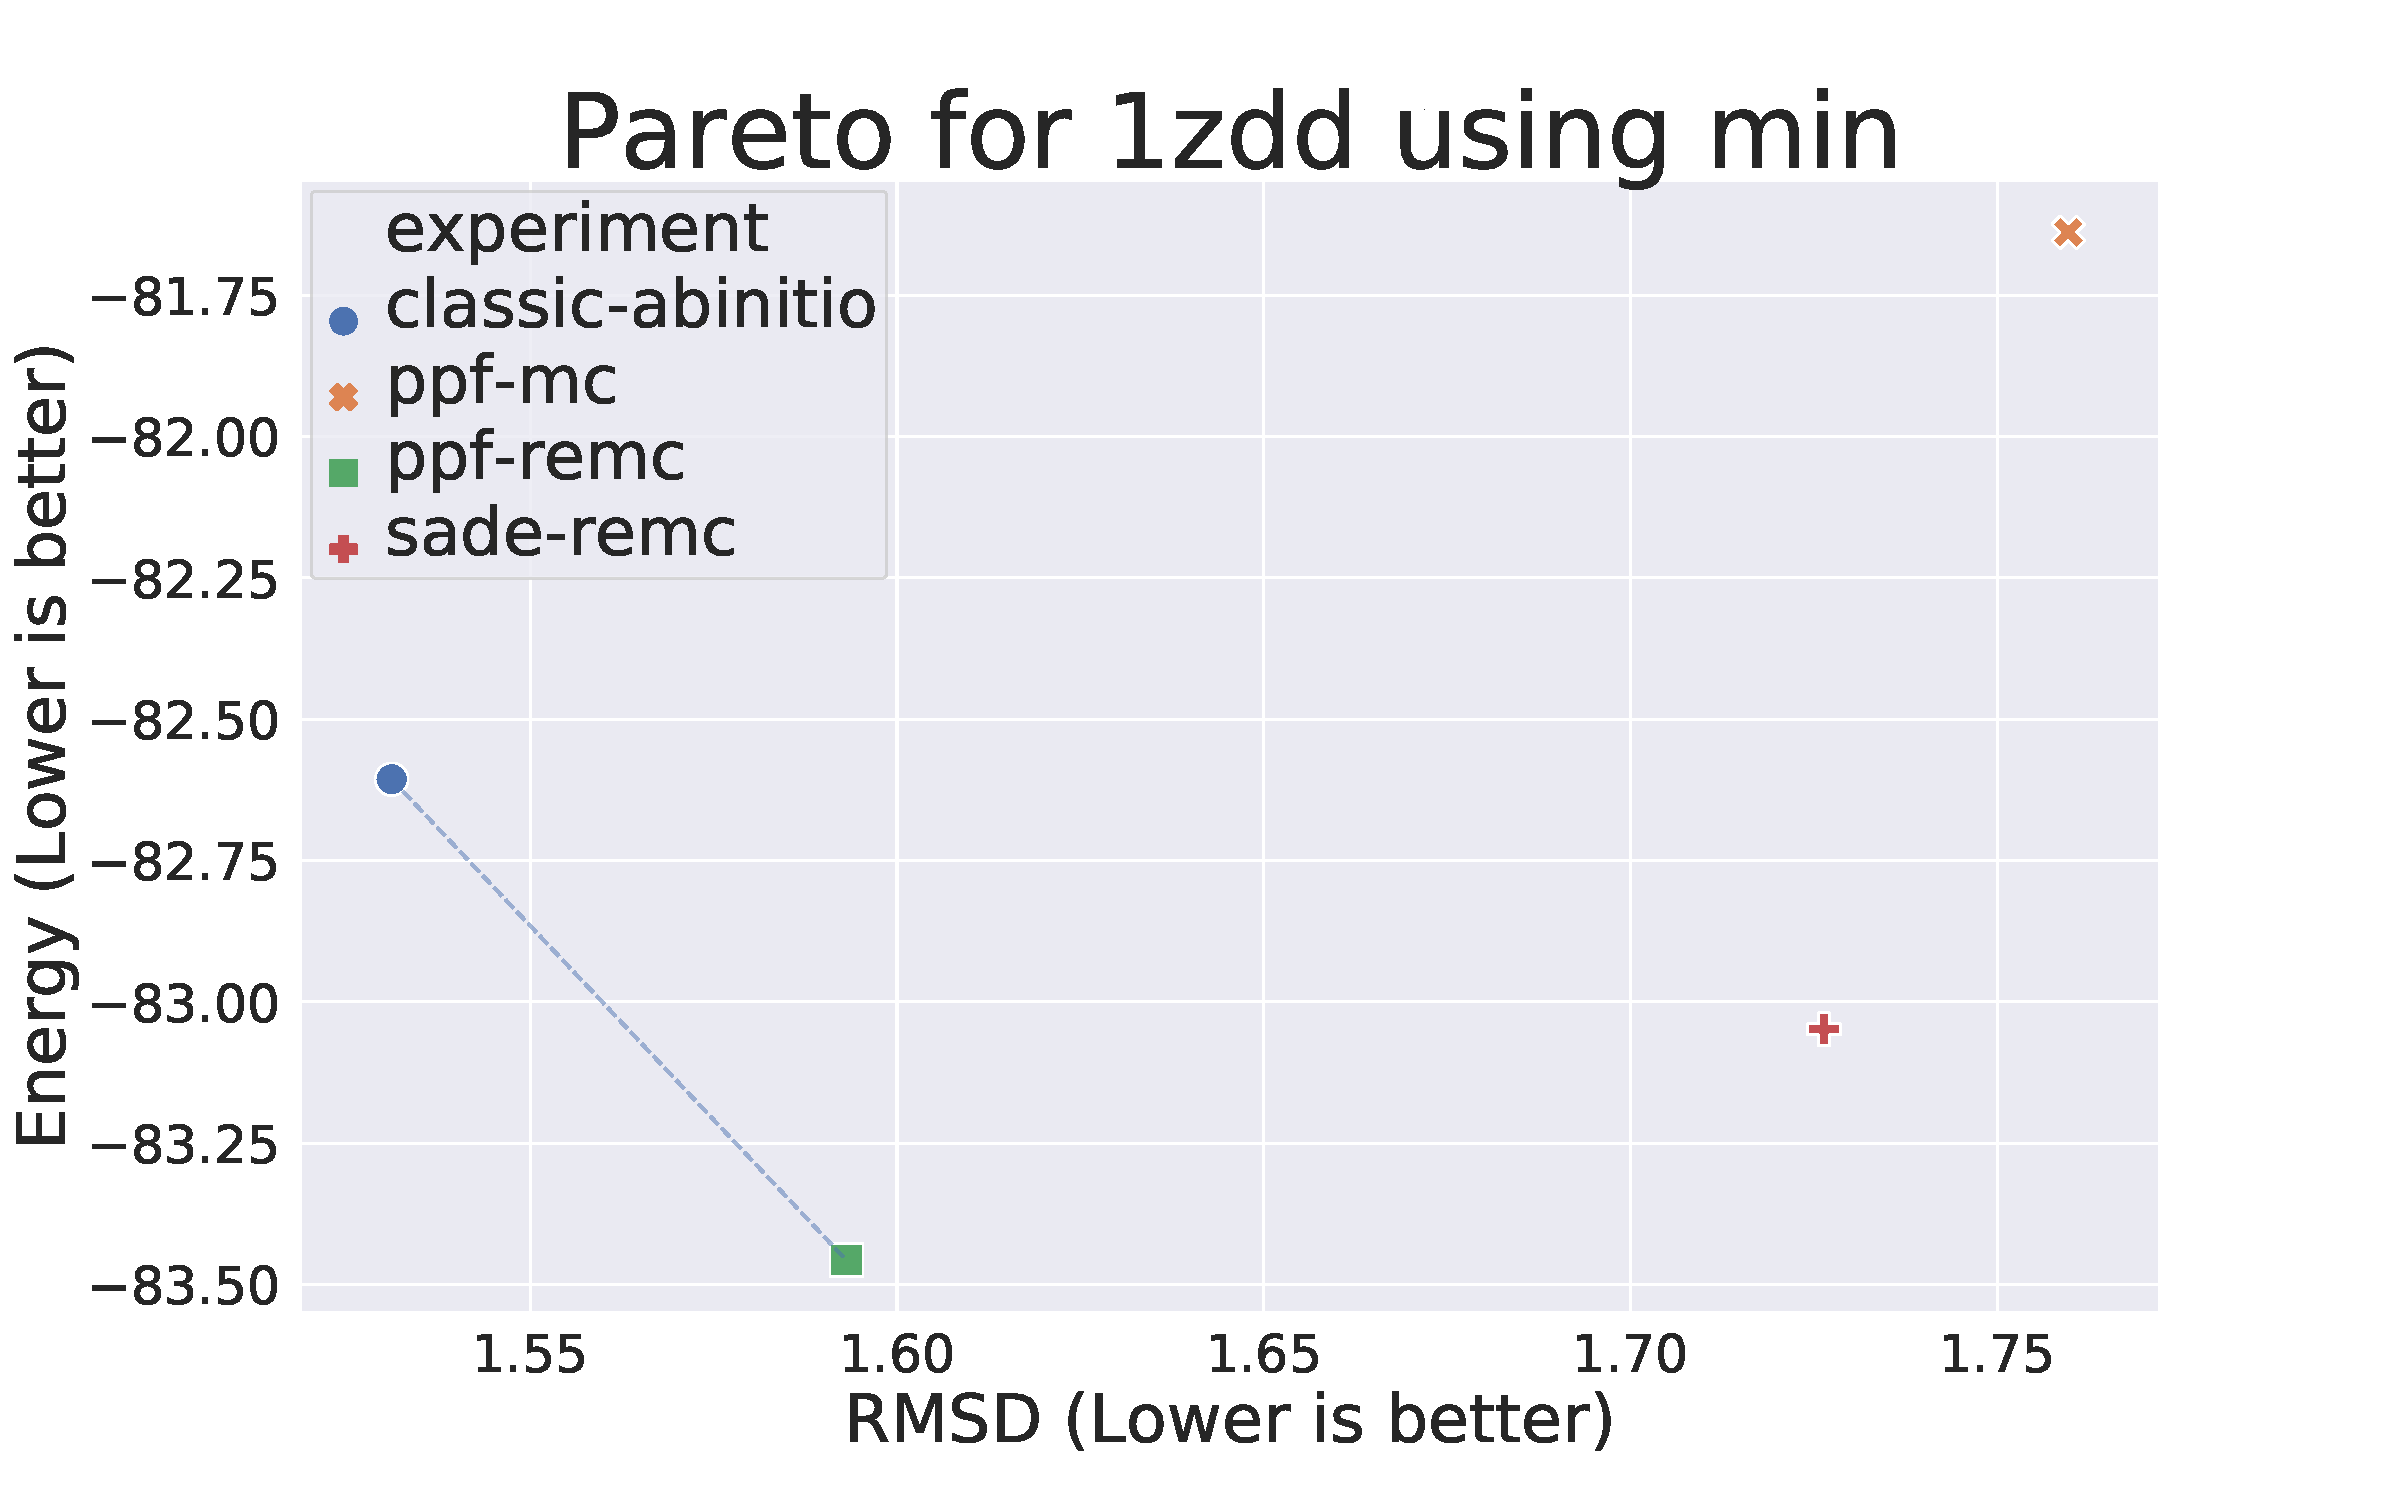
\includegraphics[width=1\linewidth]{Figuras/pareto/1zdd_best_by_rmsd_min.pdf}
  \end{subfigure}
%
  \begin{subfigure}{0.49\linewidth}
    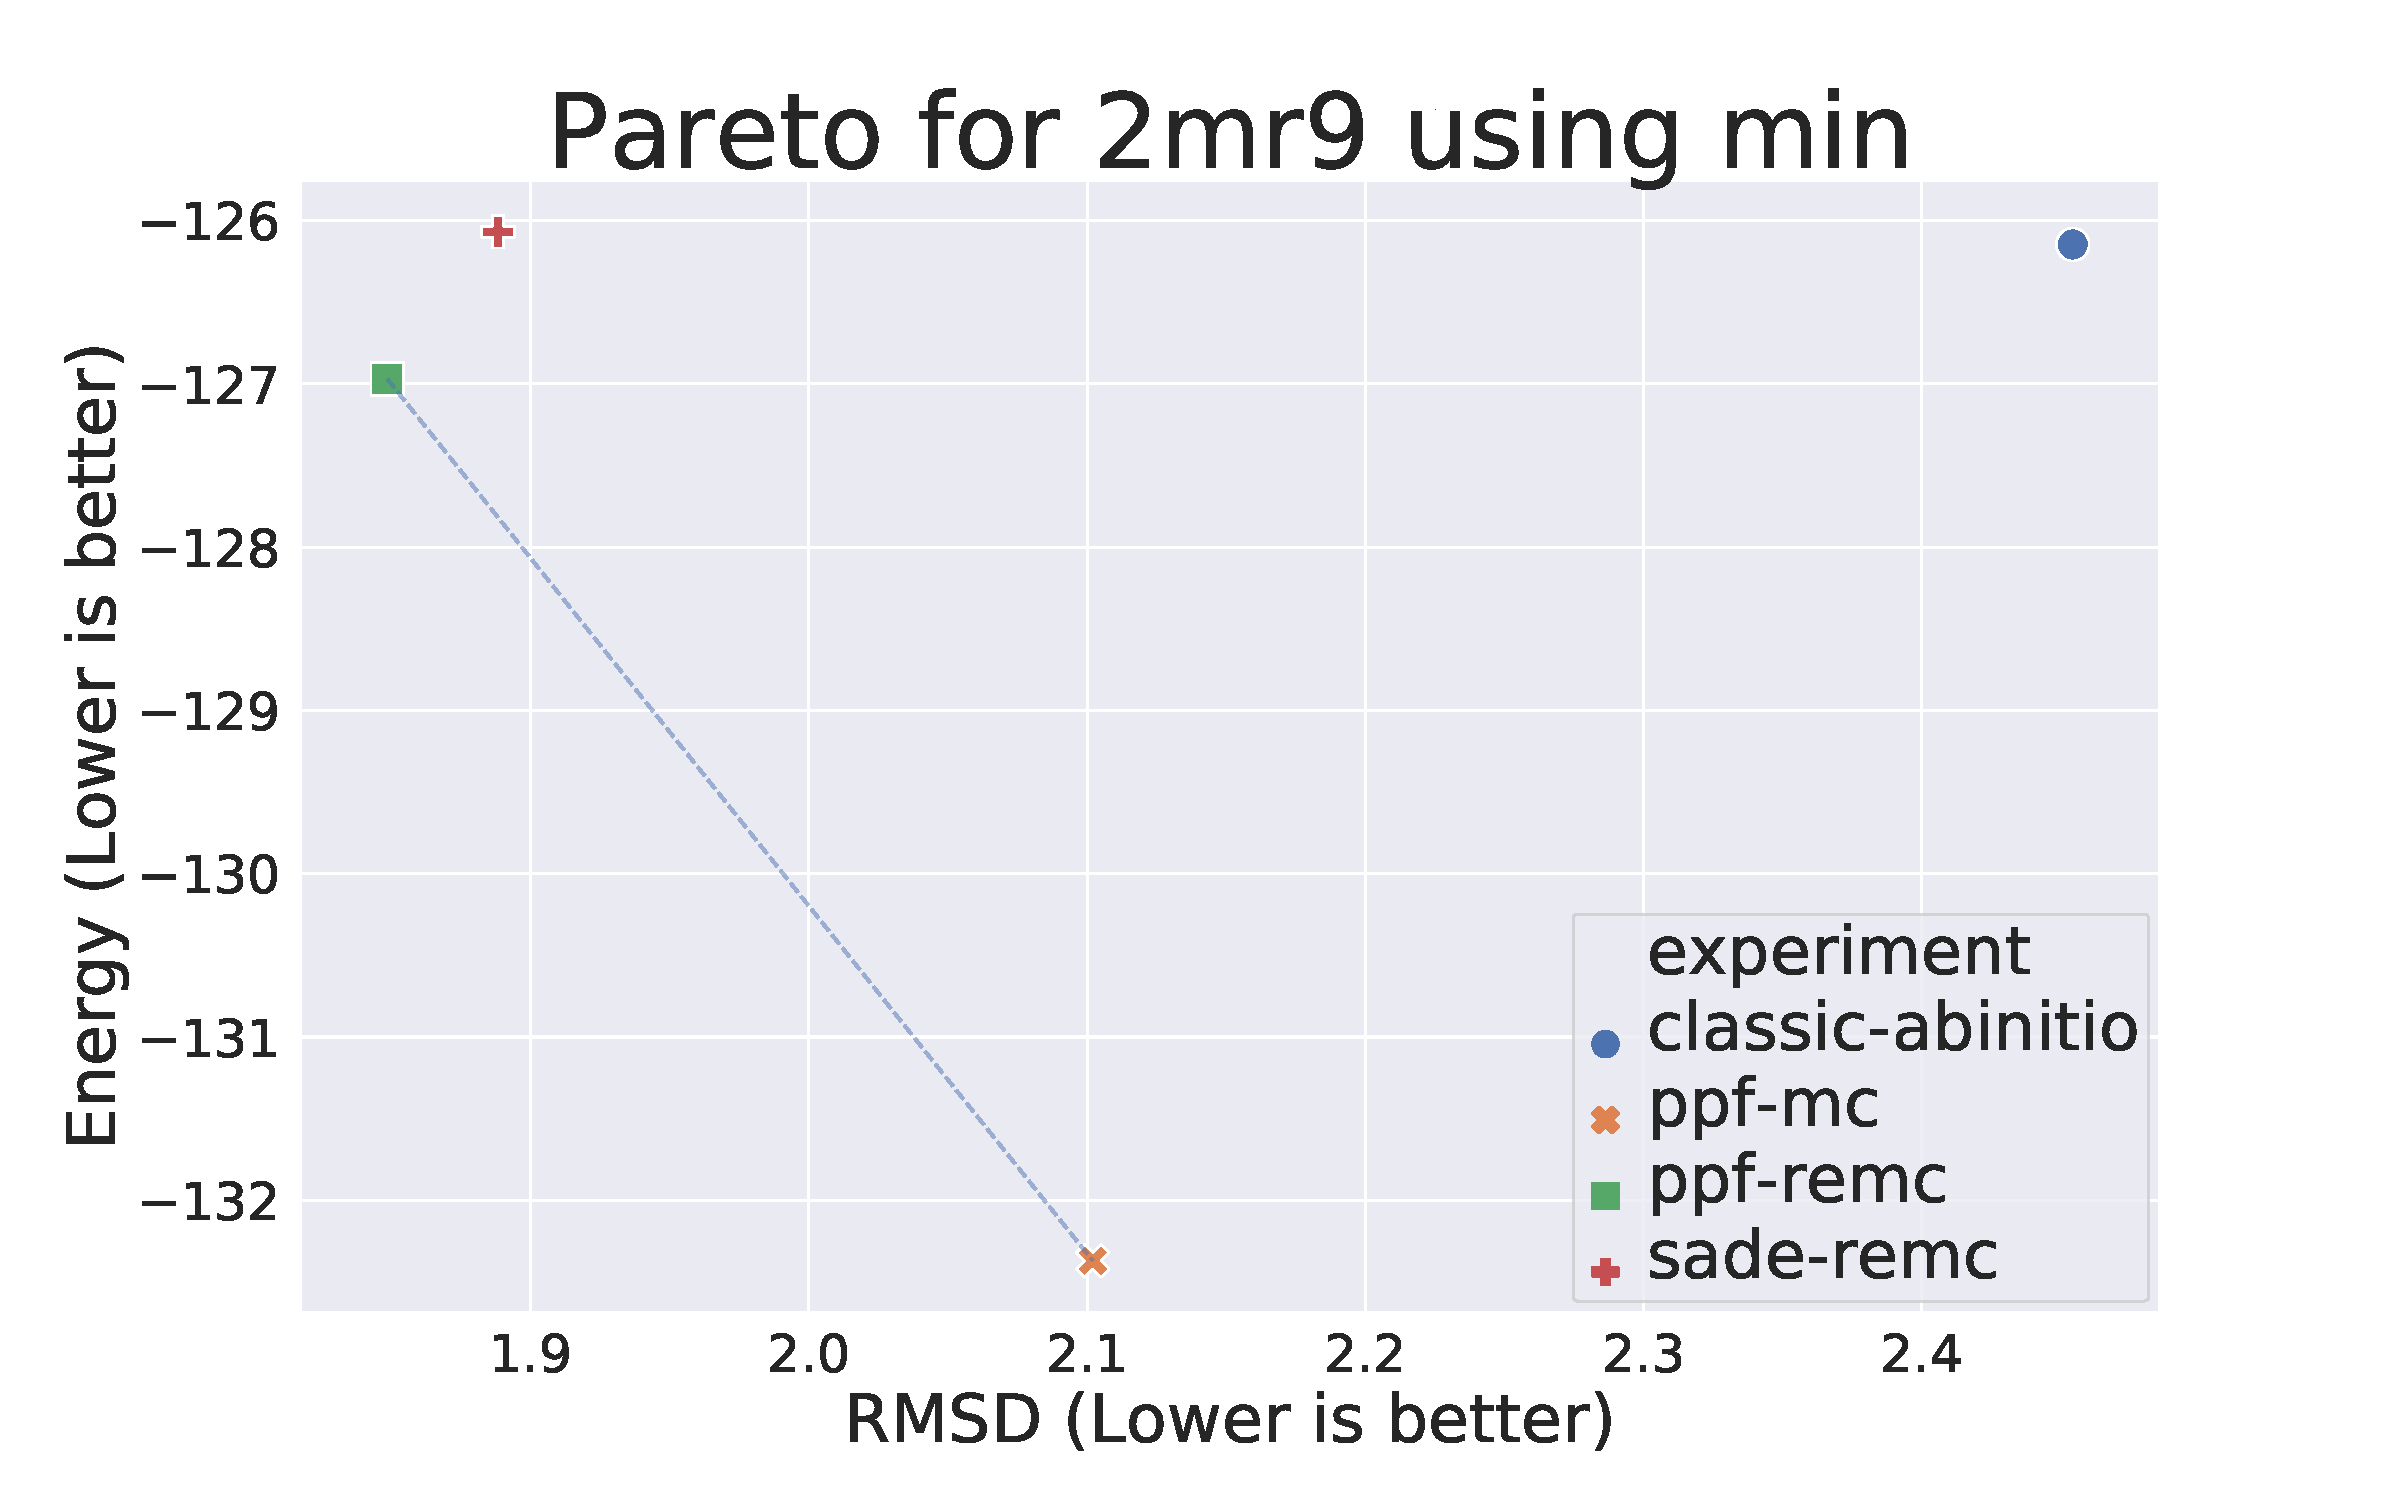
\includegraphics[width=1\linewidth]{Figuras/pareto/2mr9_best_by_rmsd_min.pdf}
  \end{subfigure}
  \caption{Pareto front of the methods using RMSD and Energy}
  \label{fig:pareto-front}
\end{figure}

The Pareto front for all 10 proteins is presented in
Figure~\ref{fig:pareto-front}. Each subfigure represents one protein.
The x-axis contains the RMSD and the y-axis contains the Energy. For proteins 1acw,
1ail, 1rop, 1zdd and 2mr9 there are two methods in the Pareto front. For
protein 1crn, there is one method which dominates all others. The remaining
proteins have three methods in the Pareto front, meaning that there is only one
method being dominated.

A summary of the which methods are present in the Pareto front is presented
in Table~\ref{tab:pareto-front-summary}. Column \textbf{Method} contains the method,
sorted by the number of times it appeared in the front. The second column,
\textbf{Proteins}, contains the proteins in which the method was in the Pareto front.
The third column, \textbf{Total}, contains the number of times the protein appeared in the
front.

\begin{table}
  \centering
  \begin{tabular}{r | r | c}
    Method    & Proteins                           & Total \\ \hline \hline
    PPF-REMC  & 1acw 1crn 1l2y 1utg 1wqc 1zdd 2mr9 & 7     \\ \hline
    PPF-MC    & 1enh 1l2y 1rop 1utg 1wqc 2mr9      & 6     \\ \hline
    rosetta   & 1ail 1enh 1l2y 1utg 1wqc 1zdd      & 6     \\ \hline
    SADE-REMC & 1acw 1ail 1enh 1rop                & 4     \\
  \end{tabular}
  \caption{Summary of the method in the Pareto front}
  \label{tab:pareto-front-summary}
\end{table}

One of the proposed methods, PPF-REMC, appeared in the Pareto front for $7$ out of 
$10$ proteins. Both rosetta and PPF-MC appeared in $6$ proteins. Finally,
SADE-REMC appeared only in $4$. On 1acw, 1crn, 1rop and 2mr9 at least one of the
proposed methods appeared in the front while rosetta did not. The converse,
rosetta being in the front while none of the proposed methods were, happened
only for 1ail.

Considering these observations, the two proposed methods and rosetta have a
similar performance regarding the Pareto front. However, rosetta was only
able to dominate the two proposed method in one occasion. Meanwhile, rosetta was
dominated in $4$.
Moreso, with the exception of 1zdd, the proposed methods
always appeared to the left of rosetta in the pareto front, indicating
a lower RMSD.
Taking this into account, it can be concluded that the two
proposed methods are able to give good conformations with varying properties
where an human expert can choose from.

\section{Convergence and Diversity Analysis}
\label{sec:convergence-analysis}

In this Section, the behaviour of the two proposed methods is analysed. The
analysis is divided in a genotipic and a phenotypic convergence analysis. The
genotipic analysis is related to how diverse the conformations are. This is
measured as the mean pairwise RMSD between all $100$ conformations in the
population. The phenotypic analysis is made considering both the energy of
the best individual and the mean energy in the population. Considering that
$50$ independent runs of each method were ran, the data to be analysed is
the mean over all runs. That is, the data on the following graphs are
the mean of mean pairwise rmsd, the mean of the best individual and the mean
of the mean population energy. Moreover, there are $20$ convergence graphs. As such,
a few select proteins are selected for analysis.
Appendix~\ref{appendix:convergence-plots} contains the plots for all 10
proteins.

\begin{figure}[ht]
  \begin{subfigure}{0.499\linewidth}
    \centering
    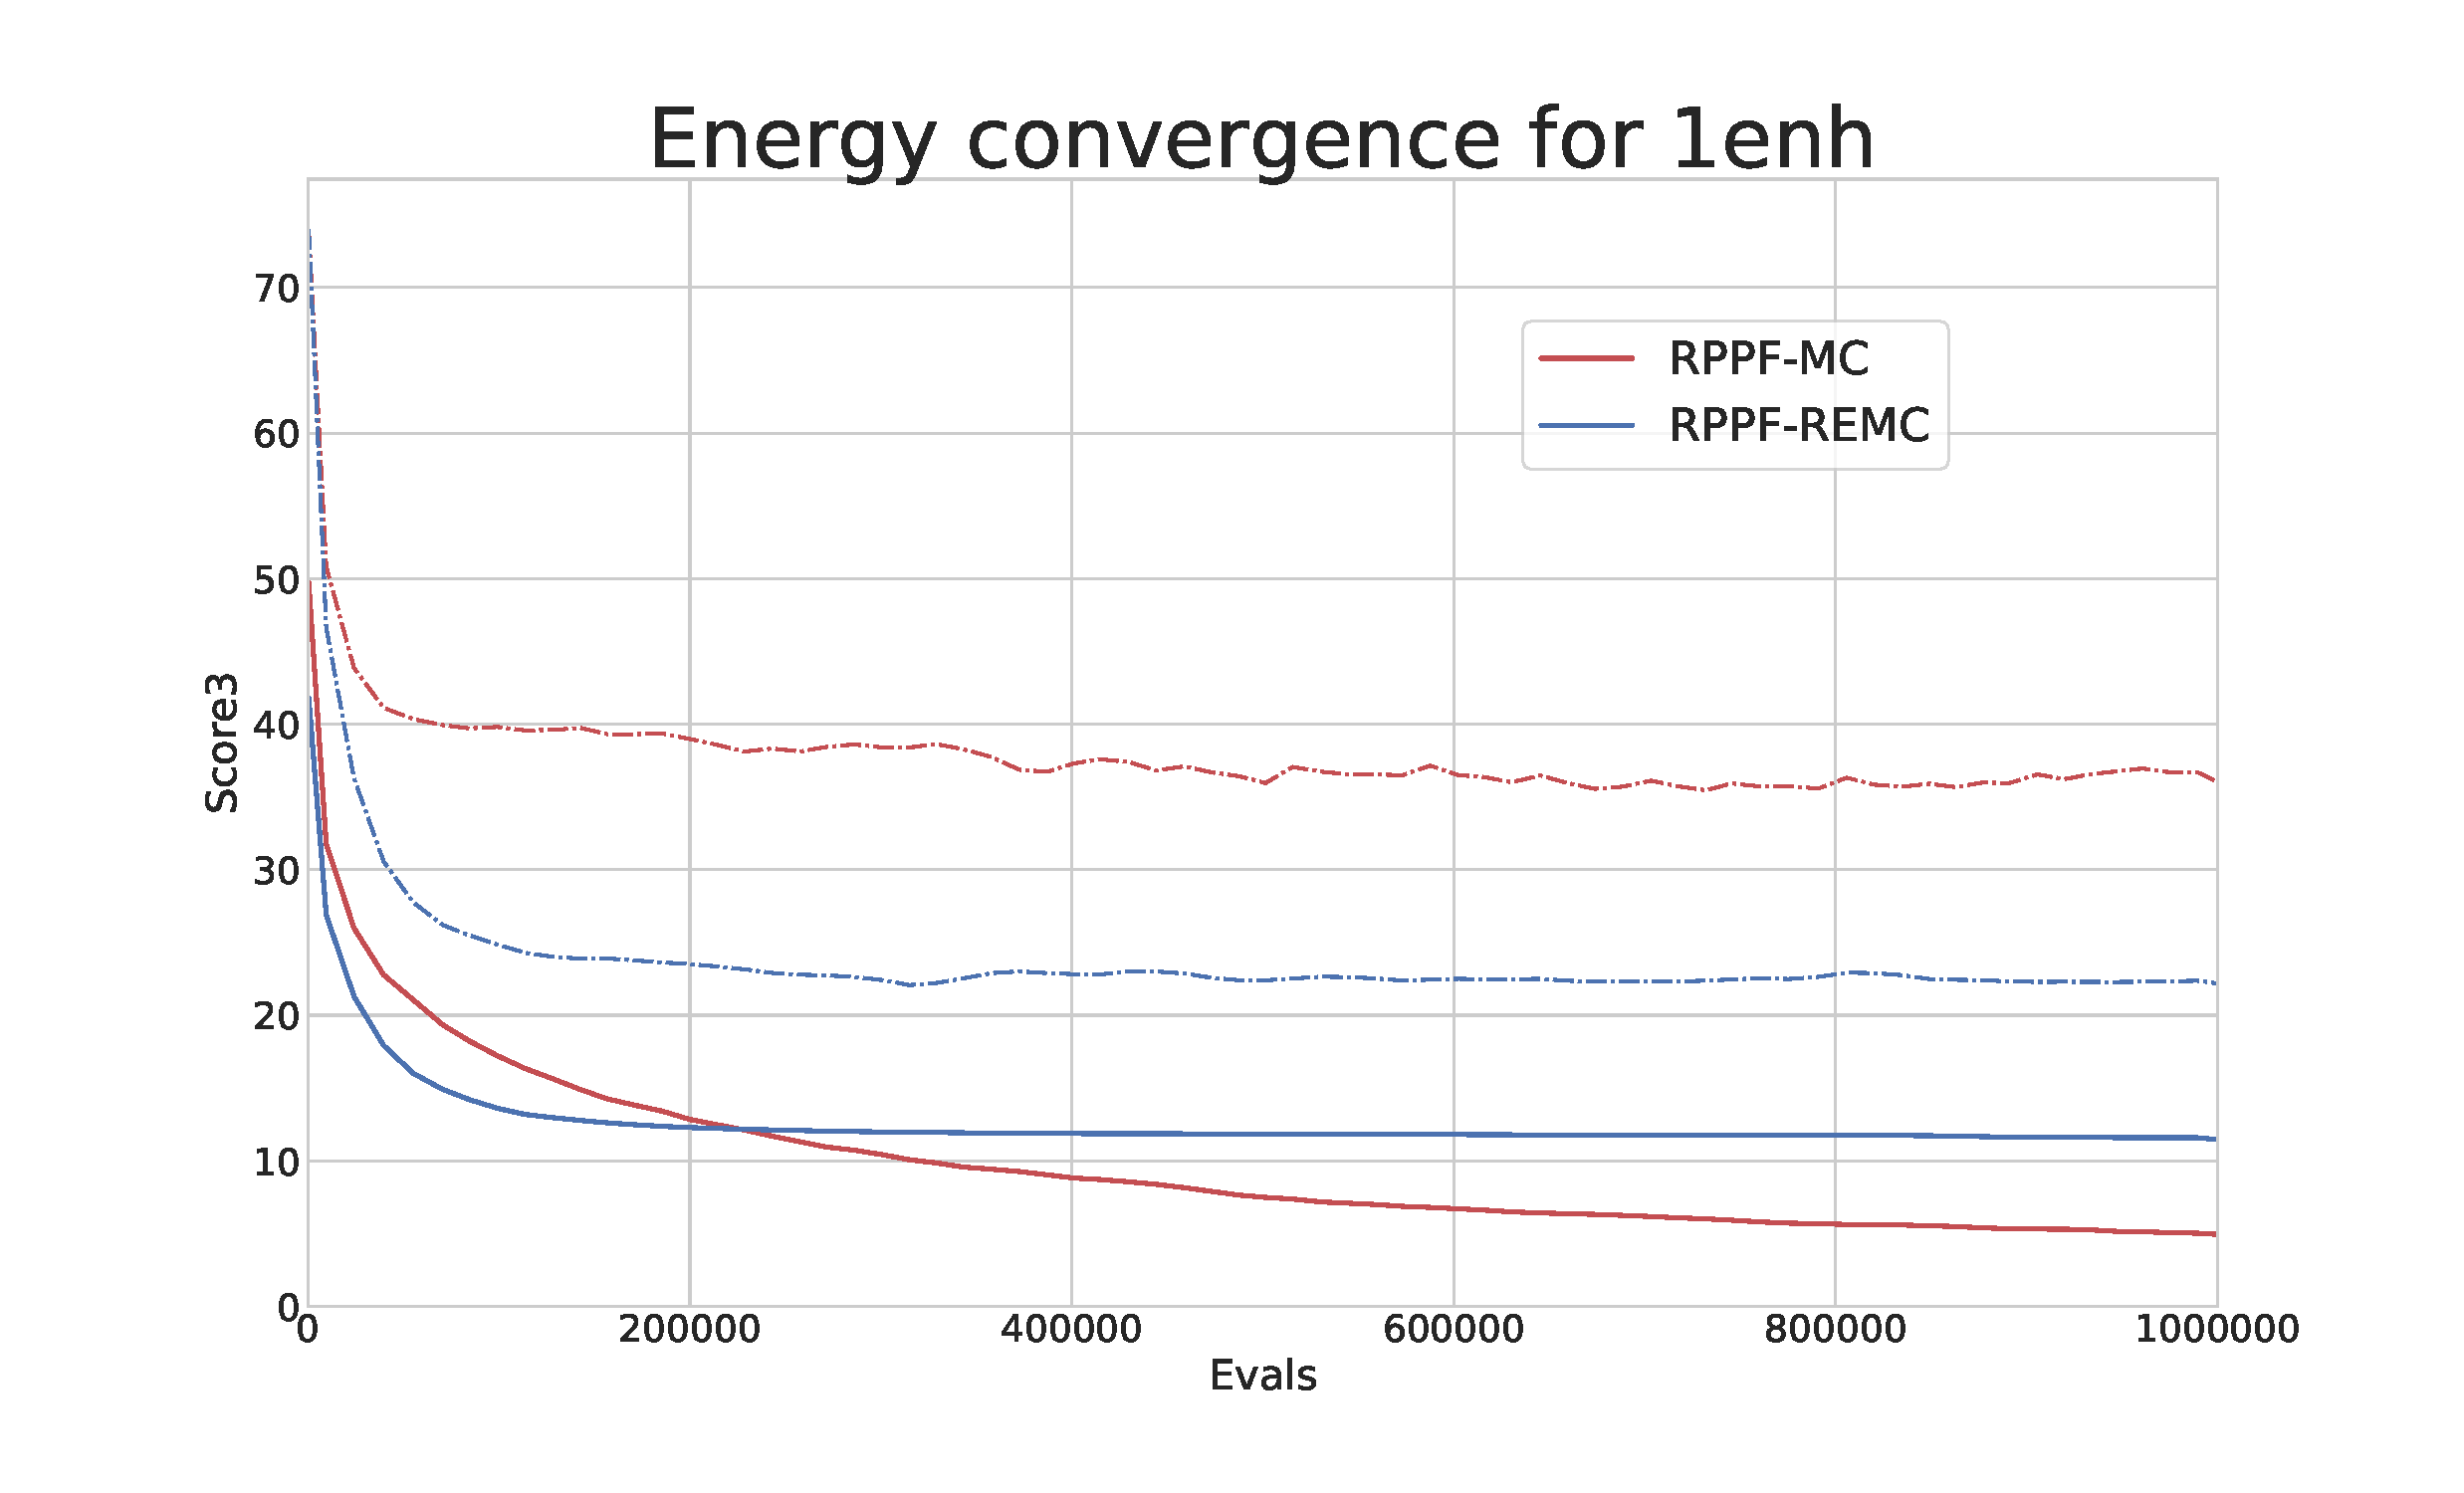
\includegraphics[width=1\linewidth]{Figuras/plots/energy_convergence/energy_convergence_1enh.pdf}
    \caption{1enh}
    \label{fig:1enh-energy-convergence}
  \end{subfigure}
%
  \begin{subfigure}{0.499\linewidth}
    \centering
    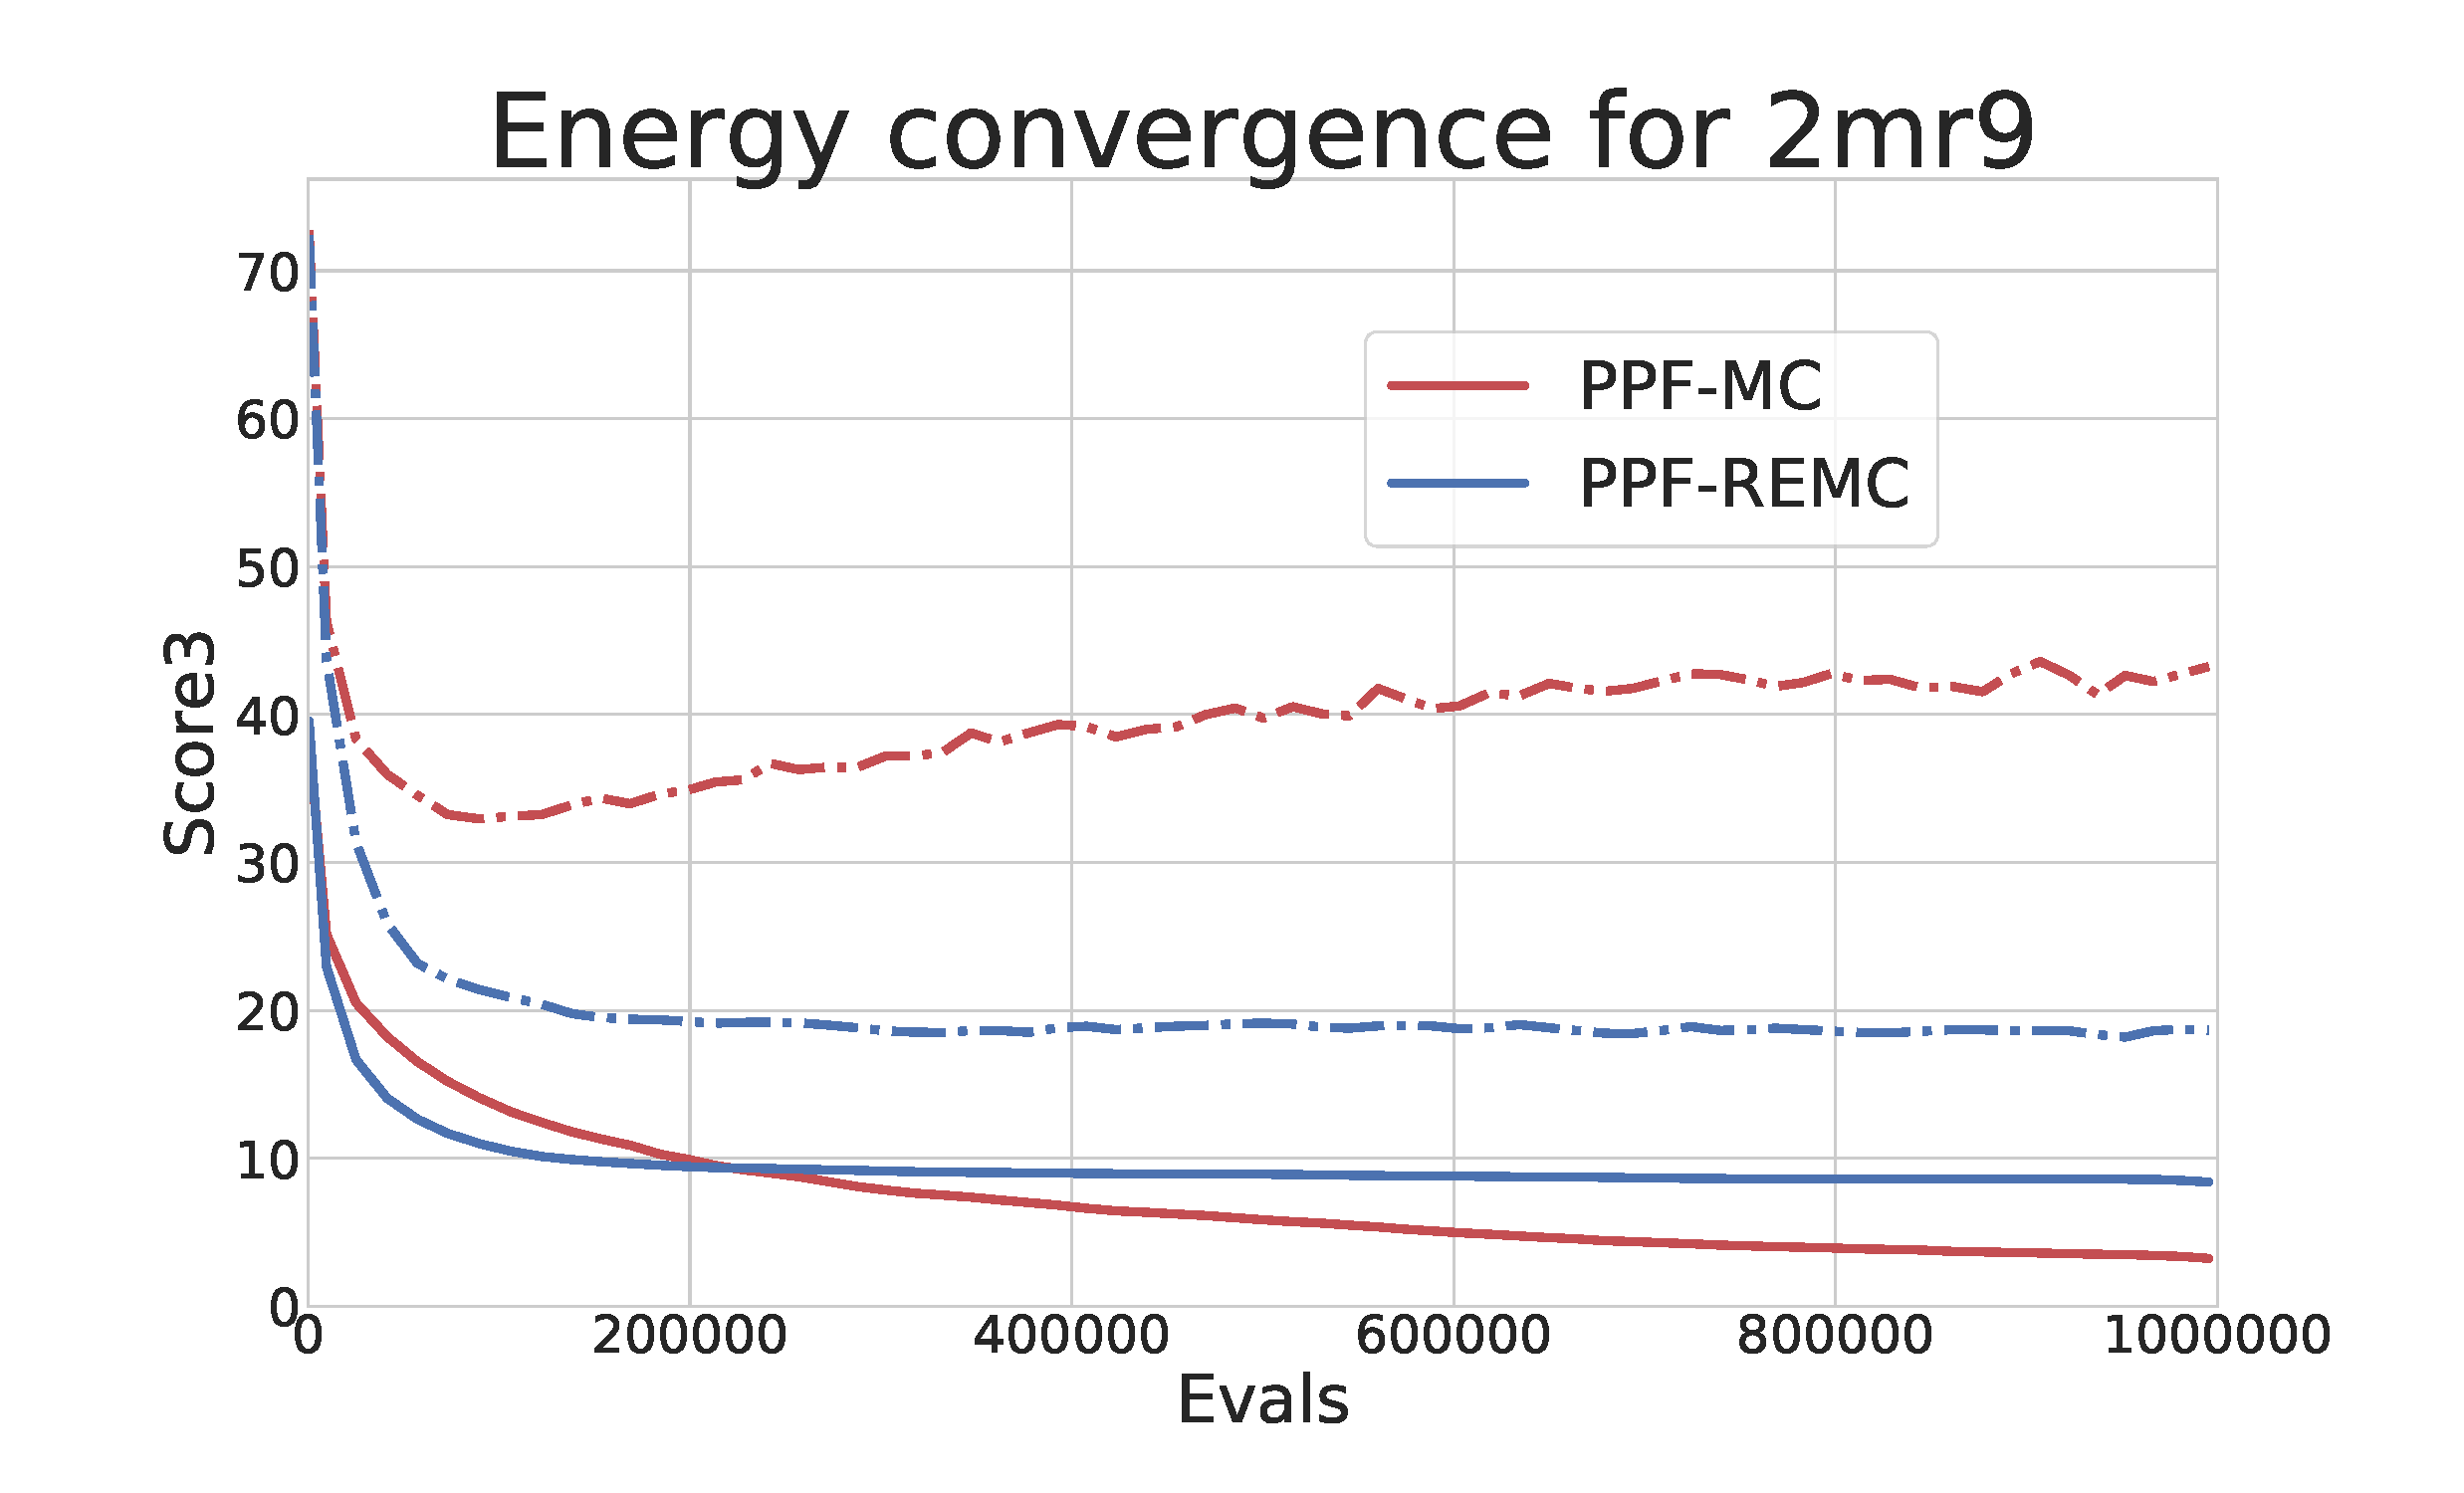
\includegraphics[width=1\linewidth]{Figuras/plots/energy_convergence/energy_convergence_2mr9.pdf}
    \caption{2mr9}
    \label{fig:2mr9-energy-convergence}
  \end{subfigure}
  \caption{The best energy and average energy for proteins 1enh and 2mr9. The
  continuous line represents the best energy. The dashed line represents the
  average of the population. The X Axis represents the function evaluations and
  the Y Axis indicates the value of the \texttt{score3} energy function being
  optimized.}
  \label{fig:energy-convergence-1enh-2mr9}
\end{figure}

In Figure~\ref{fig:energy-convergence-1enh-2mr9} the behaviour of the two
proposed methods is displayed. Protein 1enh was chosen as a representative
of standard behaviour.
There are seven other proteins with the same overall characteristics. That is,
the conclusions drawn from 1enh are also found in the other proteins.
In blue, it is possible to see that PPF-REMC has a very fast
convergence during the first 50 thousand function evaluations. After that, it
quickly comes down to a halt in convergence. This, is a classic symptom of
premature convergence. With the dashed lines, representing the average of the
population, the same overall behaviour is observable. It is worth noting that
the line is not smooth. The small "bumps" presents are caused by FFI, which
can disrupt the mean energy of the population. For PPF-MC the convergence
starts slower than for PPF-REMC, however, the best energy keeps improving
for more than three fifths of the available budget of functions evaluations.
Furthermore, on the dashed line representing the average energy, it is possible
to see that the the average improved over time as well.

When comparing PPF-MC and PPF-REMC, by looking at the best energy of the two
methods, there is a lead for PPF-REMC during the first 50 thousand function
evaluations. However, eventually PPF-MC achieves a best result and keeps
improving for the bigger part of the process. For all 10 proteins this can be
observed. Furthermore, when considering the average, PPF-REMC had the best
results in all cases.

Two of the proteins had an increase of the average populational energy over time.
This happened only for protein 2mr9 with PPF-MC. This is the reason that this
protein was selected for analysis. The best energy for both methods and the
average energy for rppc-remc shows the same behavior as 1enh. However, the
average energy for PPF-MC, after approximately 70 thousand function iterations
starts to increase until reaching a point of equilibrium at 700 thousand
function evaluations, where it starts relatively stable. This behaviour is
caused by FFI. FFI has a $2\%$ chance of being applied before any other operator
is applied. For this particular protein, FFI managed to destroy more information
than the MC fragment insertion could recover.

A similar situation happened on 1l2y, however, for the best energy for
rppc-remc. There, the best energy eventually started to increase and continued
to steadily decrease until the optimization stopped. This can also be explained
by FFI.

\begin{figure}[ht]
  \begin{subfigure}{0.499\linewidth}
    \centering
    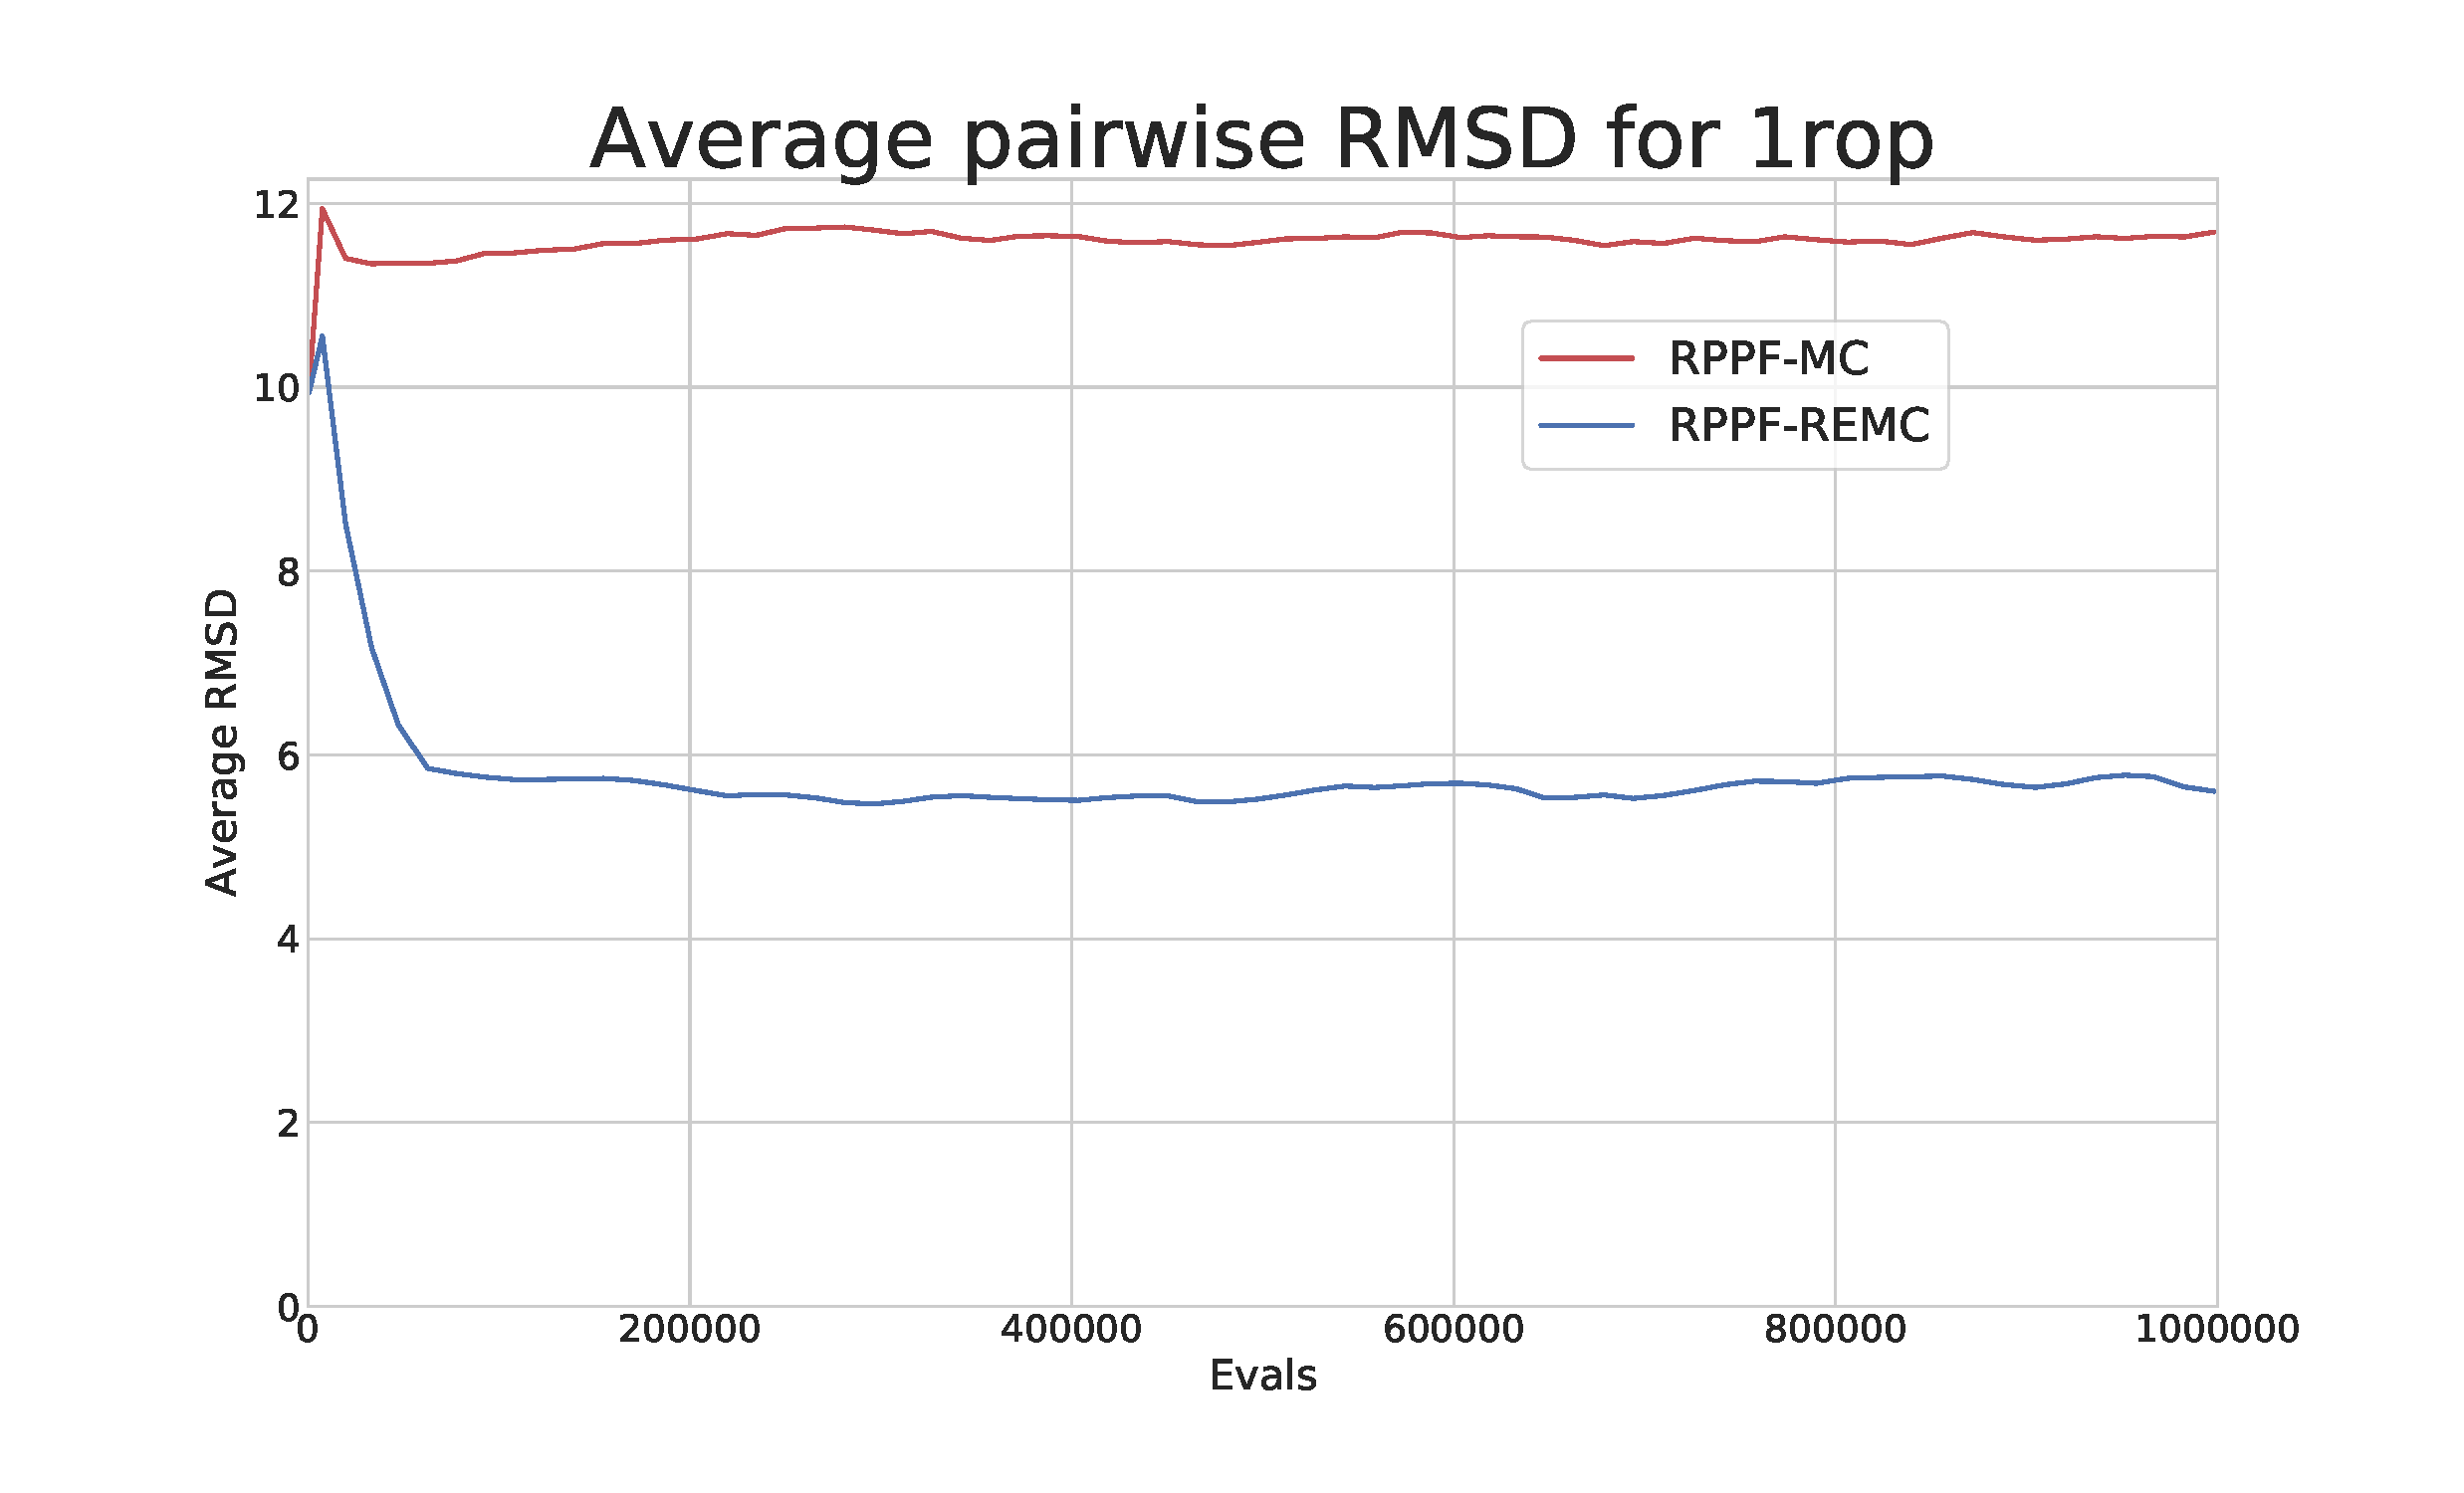
\includegraphics[width=1\linewidth]{Figuras/plots/rmsd_convergence/avg_rmsd_1rop.pdf}
    \caption{1rop}
    \label{fig:1rop-rmsd-convergence}
  \end{subfigure}
%
  \begin{subfigure}{0.499\linewidth}
    \centering
    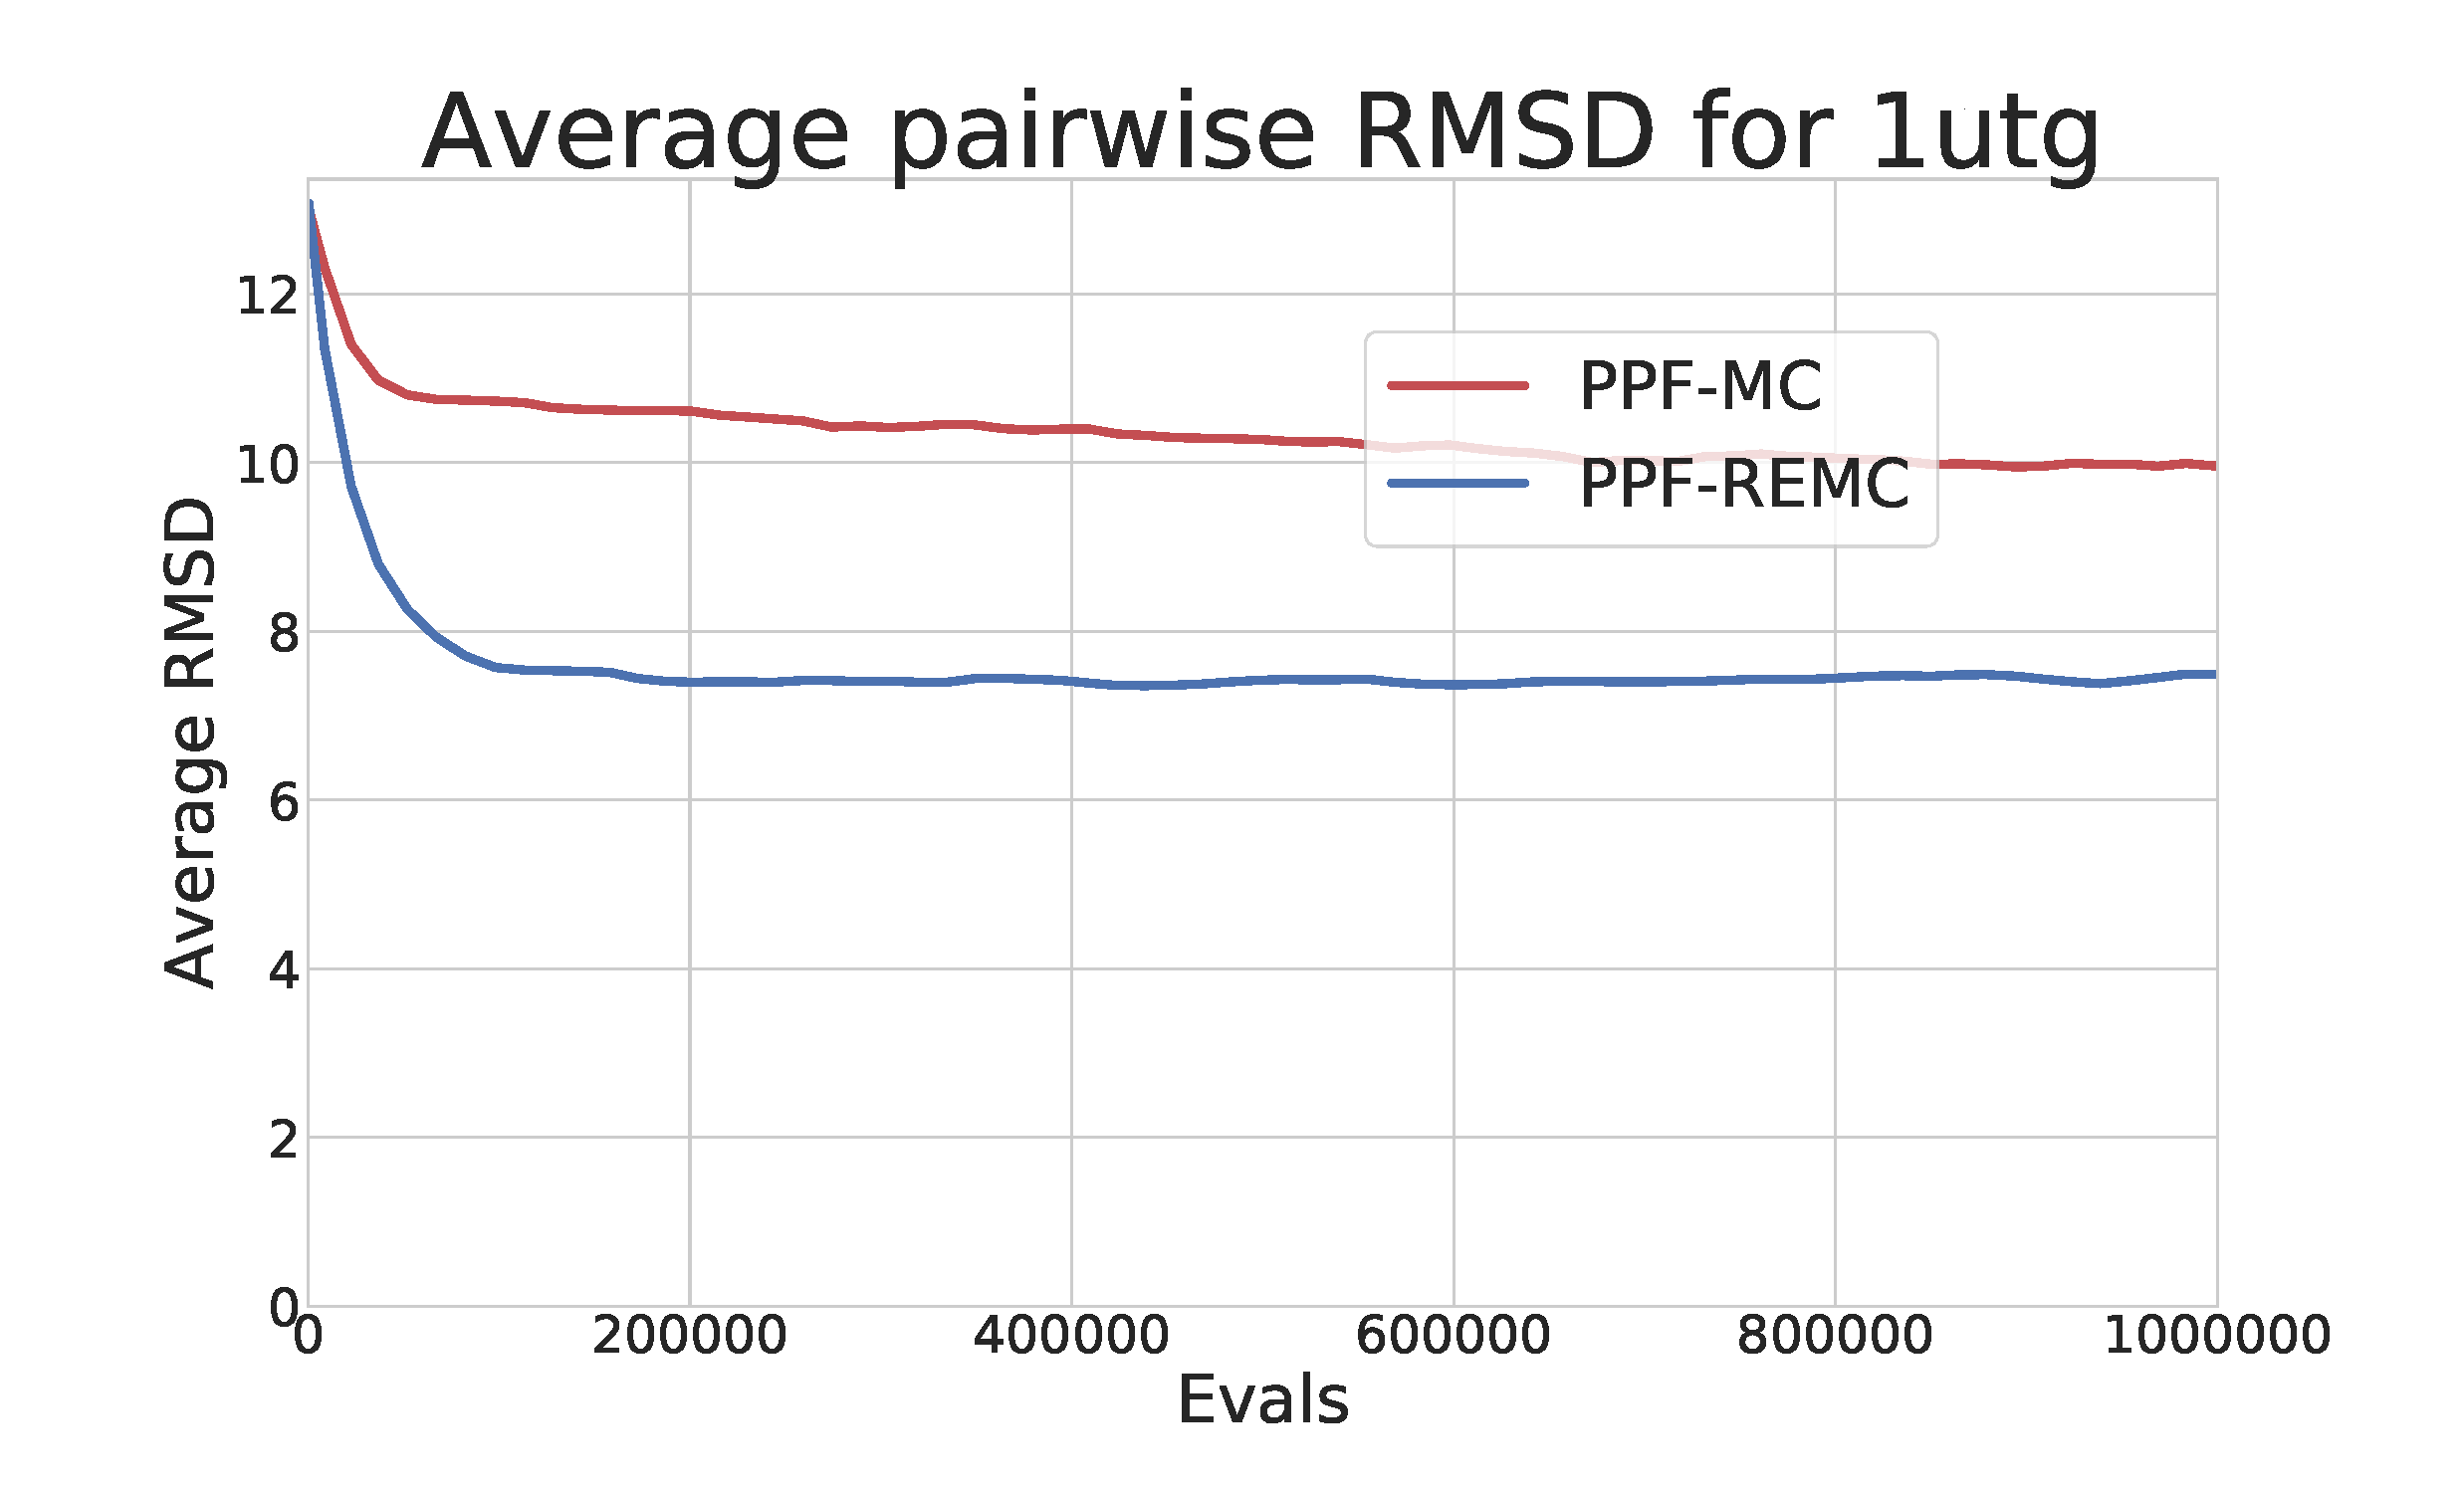
\includegraphics[width=1\linewidth]{Figuras/plots/rmsd_convergence/avg_rmsd_1utg.pdf}
    \caption{1utg}
    \label{fig:1utg-rmsd-convergence}
  \end{subfigure}
  \caption{The average pairwise RMSD for proteins 1rop and 1utg.
  The X Axis represents the function evaluations and
  the Y Axis indicates the value of the \texttt{score3} energy function being
  optimized.}
  \label{fig:rmsd-convergence-1rop-1utg}
\end{figure}

The genetopic convergence of the methods is presented in
Figure~\ref{fig:rmsd-convergence-1rop-1utg}, where the average pairwise RMSD of
the population is measured. Two proteins were selected as representatives.
Both proteins, 1rop and 1utg, have the same overall behavior as the other 8.
In both Figures~\ref{fig:1rop-rmsd-convergence}
and~\ref{fig:1utg-rmsd-convergence} PPF-REMC has a lower diversity. For 9 of
the then proteins this distance is around 2 or less. Both methods sharply
decrease the diversity during the first few thousands function evaluations.
After that, it stays relatively stable. For PPF-MC, in some proteins, such as
1utg, the diversity slowly decreases. Since there is no exchange of information
between trajectories in this method, this indicates that the whole population
is slowly converging to the same direction. The sharp decrease in diversity for
PPF-REMC is explained by its Replica Exchange mechanism, where one trajectory
can be copied to another, replacing it.

The protein where rppc-remc has the worst performance was 1rop, where it was
statistically worst than the other methods analysed. Comparing the average
diversity of both ppf derived methods, it is possible to see that there is a
gap of about $6$\AA, where the other proteins had a gap of $2$\AA  or less.
Since the population feeds the repacking stage with information, a low diversity
for such a big protein, might have lead to too many conformations being to close.
This, in turn generated clusters that are too close together.

With this analysis, is possible to detect that PPF-MC has better
convergence for the best individual than PPF-REMC. However, when considering
the average energy of the population, PPF-REMC has the best results.
Nevertheless, PPF-MC would be an interesting candidate for expanding the
budget of function evaluations available, since it keeps improving for a
longer period of time than PPF-REMC and contains a bigger overall diversity in
the population.

\section{Monte Carlo vs Replica Exchange Monte Carlo}
\label{sec:methods-duel}
% Compare PPF-MC and PPF-REMC

In this Section the two proposed methods are compared against each other, with
the goal of assessing if there is a method with a better performance. If that is
the case, then determing which one. For this, an initial visual inspection
using boxplots is first realized. Figures~\ref{fig:duel-boxplot-rmsd}
and~\ref{fig:duel-boxplot-energy} presents a direct comparison of the two
proposed methods. By inspecting the RMSD, in Figure~\ref{fig:duel-boxplot-rmsd},
it is possible to see that the two proposed methods closely match each other for
most of the proteins. For 1rop, was noticed in previous analysis, PPF-REMC was
outmatched for all other methods being analysed. In fact, as confirmed by
Kruskal–Wallis (data not shown), 1rop is the only protein where there was
a statistical significance between the two proposed method.

\begin{figure}
  \centering
  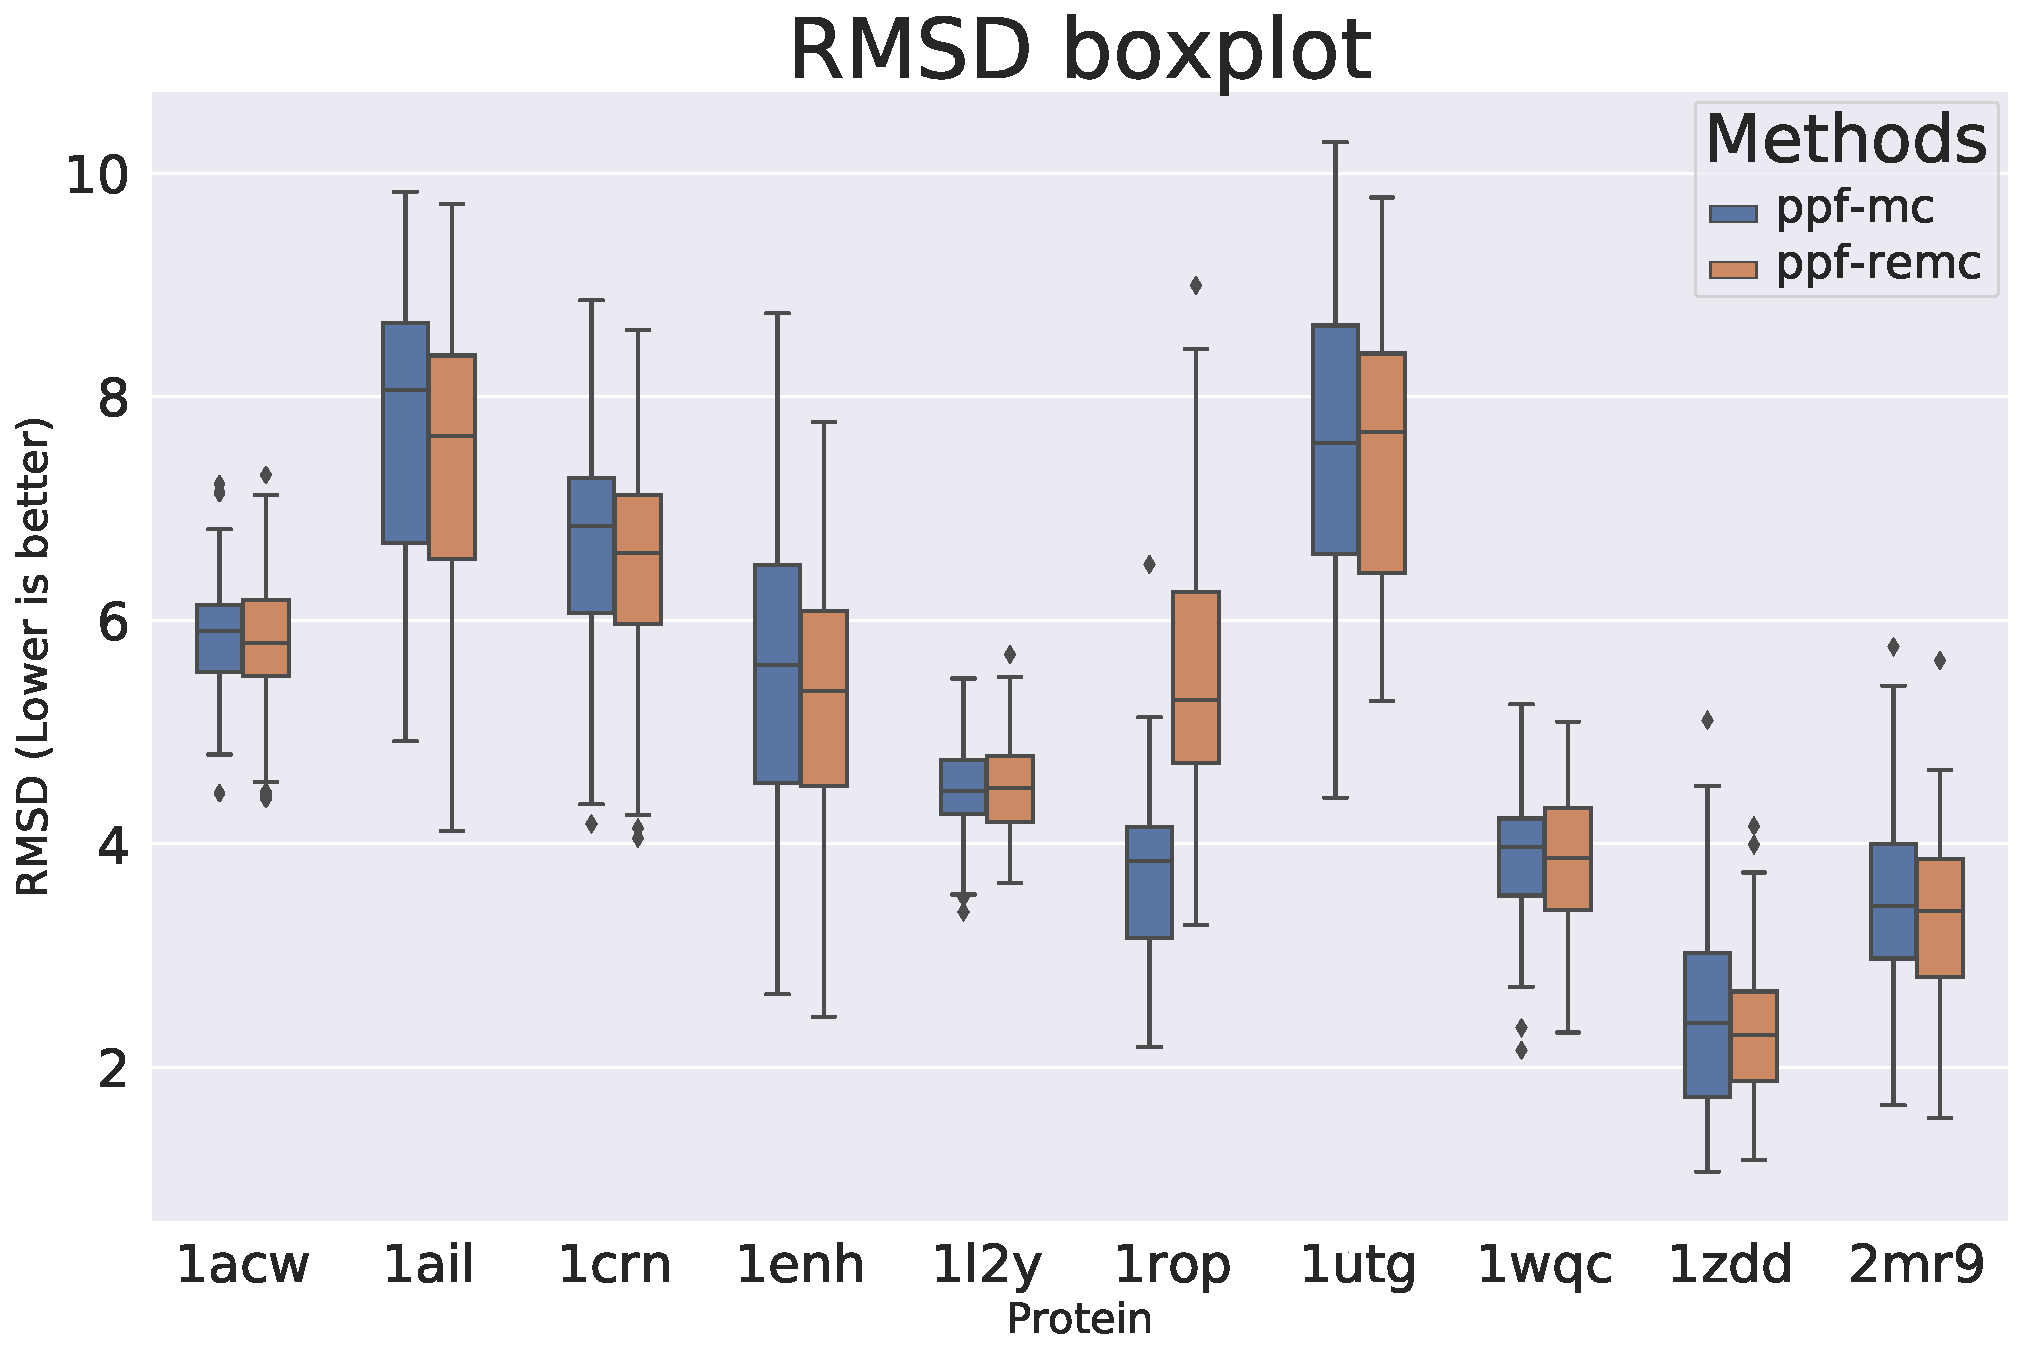
\includegraphics[width=1\textwidth]{Figuras/boxplots/duel_boxplot_best_by_rmsd_rmsd_after.pdf}
  \caption{RMSD comparison of PPF-MC and PPF-REMC.}
  \label{fig:duel-boxplot-rmsd}
\end{figure}

By analysing the Energy data, as displayed in
Figure~\ref{fig:duel-boxplot-energy}, it is possible to see that the performance
of the two proposed methods varied more than when RMSD was analysed. For protein
1rop, as expected, there is a clear difference in performance. However, for
several other proteins PPF-MC appears to have consistently reached lower
energies. In fact, by applying the Mann-Whitney test, PPF-MC outperformed
PPF-REMC for proteins 1acw, 1ail, 1enh, 1rop and 2mr9.

\begin{figure}
  \centering
  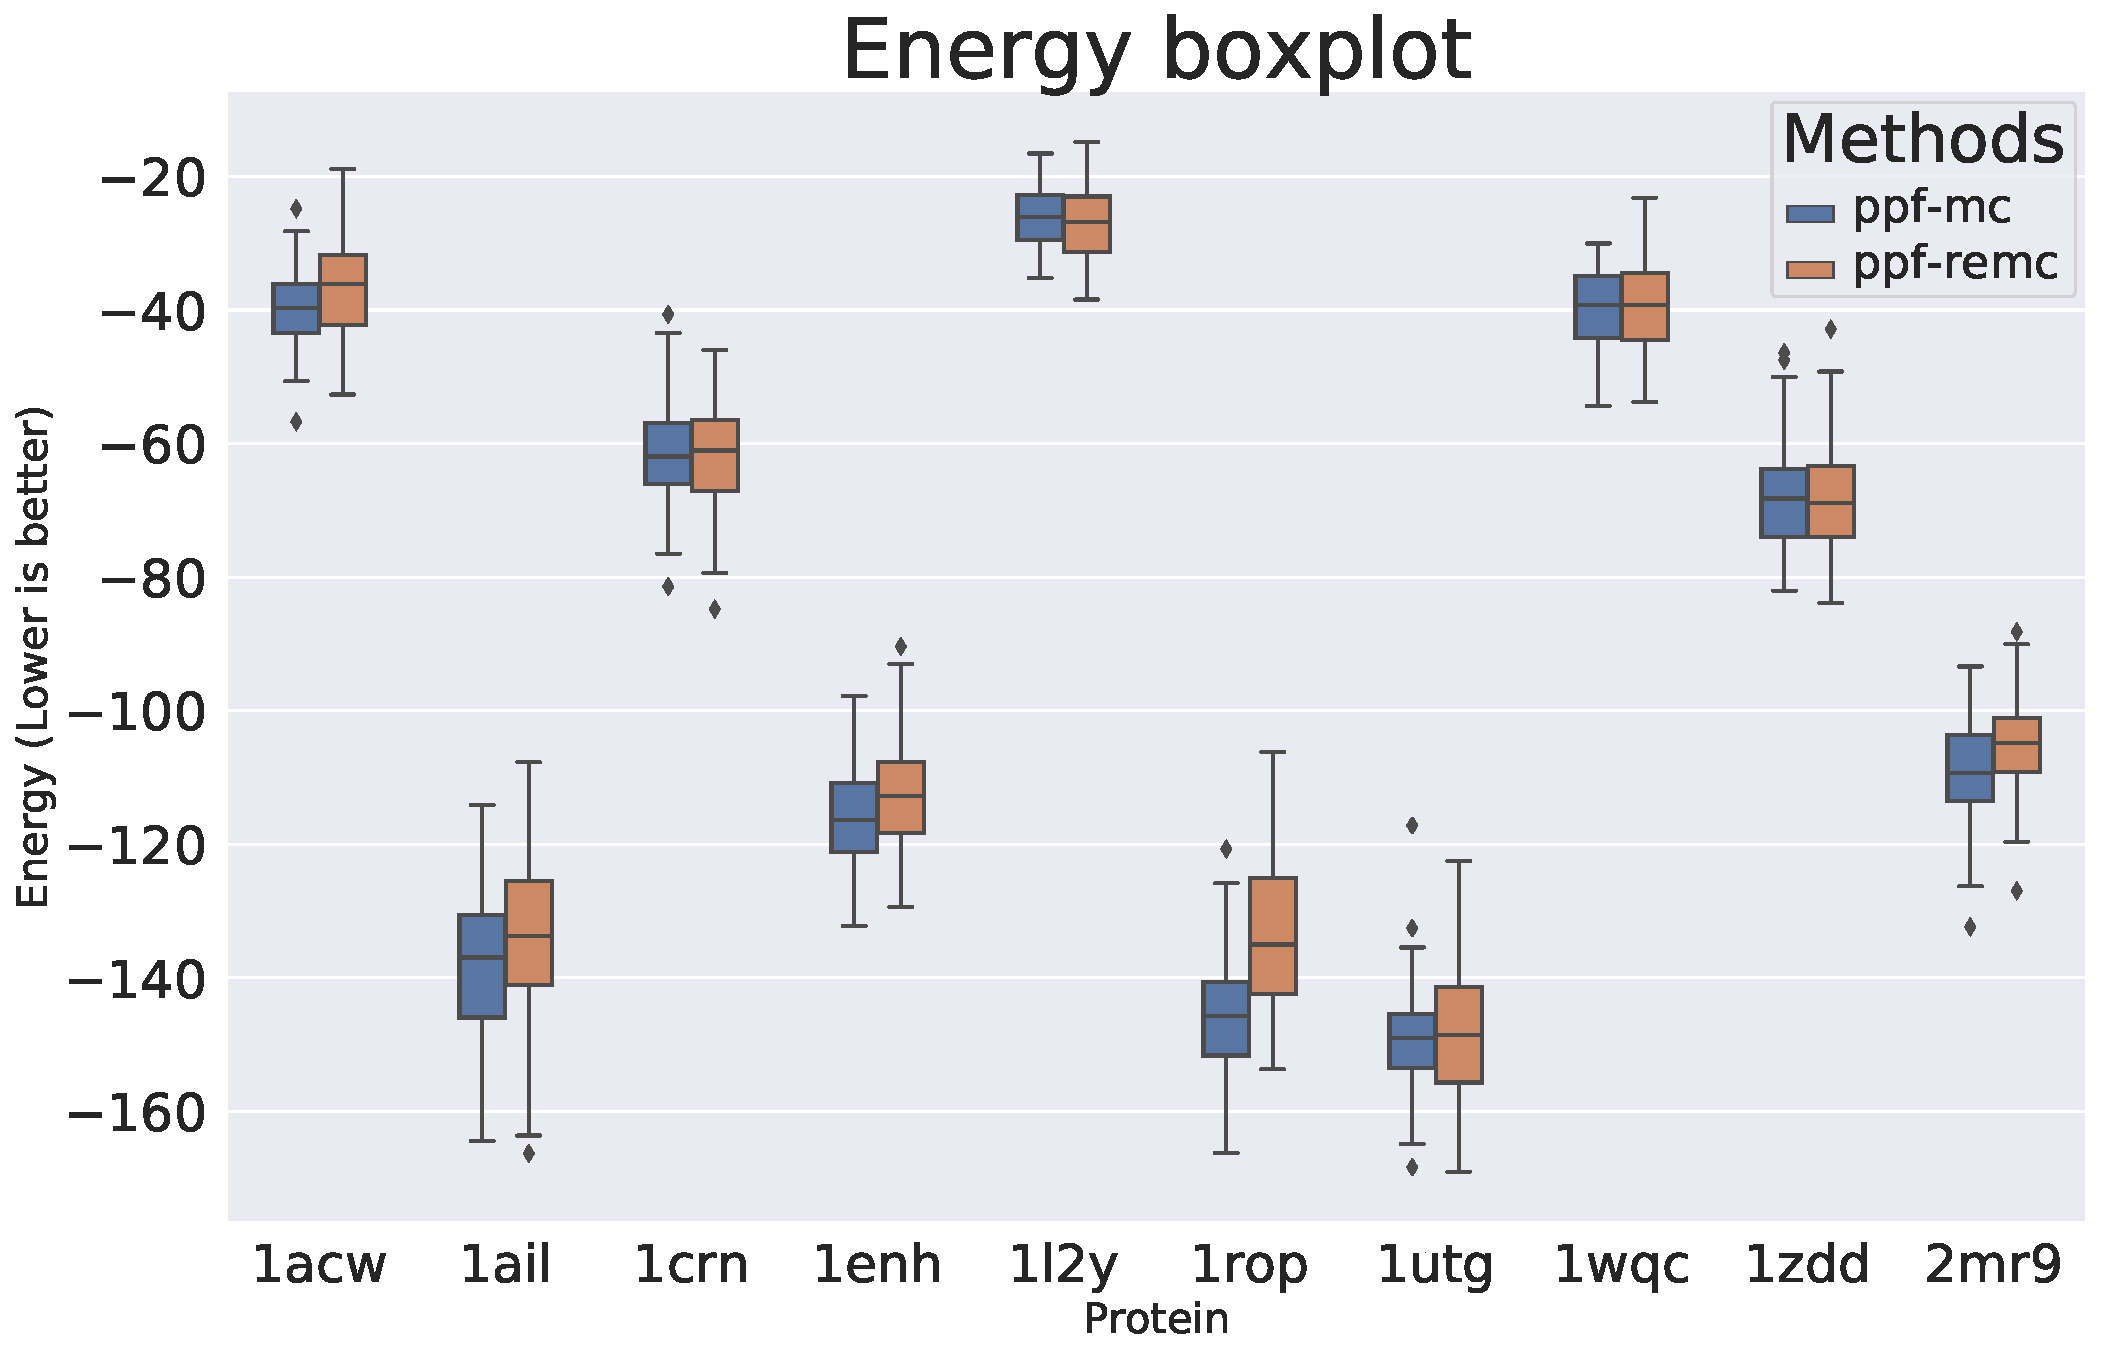
\includegraphics[width=1\textwidth]{Figuras/boxplots/duel_boxplot_best_by_energy_scorefxn}
  \caption{Energy comparison of PPF-MC and PPF-REMC.}
  \label{fig:duel-boxplot-energy}
\end{figure}

Interestingly, while PPF-MC outperformed PPF-REMC for 1 protein considering
the rmsd and on 5 proteins, it also had the best conformation prediction
prediction in 5 of proteins too (data shown in Appendix~\ref{appendix:table-results}).
Furthermore, by combining this analysis with the one
from Section~\ref{sec:convergence-analysis}, where PPF-MC had a higher
diversity, a desirable property to match with clustering, it is safe to consider
PPF-MC as the better method of the two.

\section{Repacking Impact} \label{sec:repacking-impact}
% How much does the rmsd change before after
% If ranked by energy, does the ranking change before/after repacking

A major component of the proposed methods is the use of repacking. It allows for
the method to operate on a simplified model, with side chain represented as
centroids, that has a more smooth energy landscape and is fast to evaluate. On
the other hand, this model has reduced biological plausibility. As such,
repacking allows for this centroid model to be converted to a full atomic
representation of the protein. As such, investigating the impact that repacking
has is crucial in order to understand the performance of the proposed methods.
In order to understand it, two analysis must be made, one of the RMSD, which is
straight forward. The other, for the energy, is more complex. The energies before
and after the repacking are essentially different units of measure. Therefore, a
more careful analysis is required.

\begin{table}
  \centering
  \begin{tabular}{r|r|c||r|c||r|c}
            & \multicolumn{2}{c}{classic-abinitio} & \multicolumn{2}{||c}{PPF-MC} & \multicolumn{2}{||c}{PPF-REMC} \\ \hline
    protein & mean      & stddev   & mean      & stddev   & mean      & stddev   \\ \hline \hline
    1acw    & $-0.1656$ & $0.3372$ & $0.2616$  & $0.4944$ & $0.2589$  & $0.5765$ \\ \hline
    1ail    & $-0.1113$ & $0.4629$ & $0.2470$  & $0.7731$ & $0.2379$  & $0.7278$ \\ \hline
    1crn    & $-0.0620$ & $0.4203$ & $-0.0297$ & $0.5865$ & $-0.1128$ & $0.4368$ \\ \hline
    1enh    & $-0.0558$ & $0.4854$ & $-0.1277$ & $0.5577$ & $-0.1380$ & $0.6081$ \\ \hline
    1l2y    & $0.2505$  & $0.3773$ & $0.3856$  & $0.5036$ & $0.6653$  & $0.7176$ \\ \hline
    1rop    & $0.8336$  & $0.4484$ & $0.7814$  & $0.9170$ & $1.2214$  & $1.3530$ \\ \hline
    1utg    & $-0.3506$ & $0.4712$ & $0.1346$  & $0.5762$ & $0.1793$  & $0.7202$ \\ \hline
    1wqc    & $-0.2543$ & $0.4381$ & $0.1729$  & $0.5624$ & $0.2160$  & $0.6377$ \\ \hline
    1zdd    & $0.2283$  & $0.4144$ & $0.7429$  & $0.6098$ & $0.7470$  & $0.9897$ \\ \hline
    2mr9    & $-0.2667$ & $0.6094$ & $0.2190$  & $0.5679$ & $0.1875$  & $0.6957$ \\ \hline
  \end{tabular}
  \caption{RMSD change caused by repacking}
  \label{tab:repack-impact-rmsd}
\end{table}

Table~\ref{tab:repack-impact-rmsd} presents the RMSD delta from before and after
the repacking. A negative delta value indicated that repacking increased the RMSD,
i.e. made it worse. Conversely, a positive value indicates that the RMSD decreased,
i.e. improved.
Since the proposed methods are mainly compared against rosetta,
it was included here as well. With this, it is possible to detect if repacking
gave unfair advantage to any of the three methods. A few patterns are detected
in the results. Firstly, both 1crn and 1enh had a increase of RMSD. While
relatively small, specially for rosetta, it is interesting that it happened for
the two proteins for all three methods. No other protein has this happen.
Another interesting point is that with the exception of 1l2y, 1rop and 1zdd,
rosetta had an increase of RMSD for all the remaining seven proteins. The
biggest mean difference was on 1utg, with a value of $-0.3506$. Comparing these
results with the medians from Table~\ref{fig:boxplot-rmsd} shows that the
impact of repacking for the RMSD has no impact in the statistical tests. Rosetta,
for 1utg, had a median above $10$, while the two proposed methods had a median
below $8$. Finally, the third noteworthy aspect of the results is that the only
mean above $1$ was on 1rop for PPF-REMC, which had the worst performance
on that protein. This result could be explained due to the method having poor
optimization performance for this particular case. As such, repacking had more
room for improvement.

The energy impact of using repacking is more complex to conduct. As an
alternative of doing a direct delta of the values before and after, it is
possible to apply the same statistical analysis from
Section~\ref{sec:methods-analysis}. The results can then be compared
against Table~\ref{tab:mann-whitney-summary-rosetta-best-by-energy-scorefxn}.
If the repacking procedure had an unfair advantage to any of the methods
it will be detectable.

\begin{table}
  \centering
  \begin{tabular}{r|r|r|r}
  Protein & Wins & Loses & Draws \\ \hline \hline
   1acw &  2 &  0 &  0 \\ \hline
   1ail &  0 &  0 &  2 \\ \hline
   1crn &  1 &  1 &  0 \\ \hline
   1enh &  1 &  0 &  1 \\ \hline
   1l2y &  2 &  0 &  0 \\ \hline
   1rop &  2 &  0 &  0 \\ \hline
   1utg &  2 &  0 &  0 \\ \hline
   1wqc &  2 &  0 &  0 \\ \hline
   1zdd &  2 &  0 &  0 \\ \hline
   2mr9 &  2 &  0 &  0 \\ \hline
  \end{tabular}
  \caption{Summary of Mann-Whitney using score3, using the energy before repacking.
  The two proposed methods are compared agaisnt rosetta.}
  \label{tab:mann-whitney-summary-best-by-energy-score3}
\end{table}

The same sequence of statistical tests from
Section~\ref{sec:methods-analysis} were applied again, but now, only
considering the energy from before repacking, as scored by~\texttt{score3}.
In order to keep the analysis short, yet complete, only a summary of the
results is provided, presented in
Table~\ref{tab:mann-whitney-summary-best-by-energy-score3}.
This table can directly be compared against
Table~\ref{tab:mann-whitney-summary-rosetta-best-by-energy-scorefxn}.
It is worth noting that the results from Kruskal–Wallis (not shown) returned that there is
statistical difference for all the proteins, therefore, all proteins are
considered this time.

With the energy data from after the repacking, there were $2$ proteins,
2mr9 and 1utg, where the
two proposed methods outperformed rosetta. Using the data from before, there are
$7$ proteins (1acw, 1l2y, 1rop, 1utg, 1wqc, 1zdd and 2mr9).
A clear indicator that repacking had a considerable impact in the
energy of the final conformations. Furthermore, with \texttt{scorefxn} there
were two times were rosetta outperformed one of the proposed methods, with
\texttt{score3} there is only one. The number of draws between rosetta and the
proposed methods was also reduced. With \texttt{scorefxn} there were $12$
occurrences, while for \texttt{score3} here are $3$.

With these results, it is clear that repacking had a significant impact in the
energy of the final predicted conformations. By applying repacking, which is
essentially another optimizer, the results of the proposed methods and rosetta
reached close energy distributions several times. Nevertheless, even with
repacking the proposed methods were able to outperform rosetta in multiple
occasions. With this, it can be concluded two main points. Firstly, using
repacking did not benefit only the proposed methods. Secondly, repacking
appears to impact more the energy than RMSD.

\section{Processing time and functions evaluations} \label{sec:time-and-evals}

In Table~\ref{tab:processing-times} the processing times for the two proposed
methods are displayed. The first column shows the protein name, the second and
third column show the data for each of the methods. Each sub-column for the
methods contains the mean time and its standard deviation, measured in seconds.
The total processing time of the method does not include the preprocessing
steps, i.e. secondary structure prediction, the fragment picker, etc. The total
time considered is the sum of several steps of the algorithm. The time starts
counting for the main optimization phase when the initial population is
generated and it stops when the defined 1 million function evaluations is
spent. Then, the post processing phase starts, which is divided into three
sub steps. The first is the clustering, which overall averages less than a
second by itself. The second step is running Hooke-Jeeves for all the
conformations nearest to the cluster centroids. The final step is applying
repacking to the resulting conformations from Hooke-Jeeves. The final
processing time is the sum of all these steps.

\begin{table}
  \centering
  \begin{tabular}{r|c|c||c|c}
            & \multicolumn{2}{c}{PPF-MC} & \multicolumn{2}{||c}{PPF-REMC} \\ \hline
    protein & mean & stddev & mean & stddev \\ \hline \hline
    1acw & $ 381.8566$ & $ 76.8664$ & $ 397.3399$ & $ 39.2449$ \\ \hline
    1ail & $1141.1461$ & $142.2935$ & $1127.3899$ & $139.9729$ \\ \hline
    1crn & $ 721.0492$ & $118.6126$ & $ 696.0591$ & $ 78.4302$ \\ \hline
    1enh & $ 763.7677$ & $ 86.2599$ & $ 783.4028$ & $ 95.5297$ \\ \hline
    1l2y & $ 252.8980$ & $ 19.1262$ & $ 252.7463$ & $ 18.8516$ \\ \hline
    1rop & $ 963.2695$ & $124.7610$ & $ 940.5557$ & $203.5212$ \\ \hline
    1utg & $1010.0412$ & $142.8927$ & $1018.6922$ & $193.5863$ \\ \hline
    1wqc & $ 341.4484$ & $ 35.1510$ & $ 346.3862$ & $ 36.6248$ \\ \hline
    1zdd & $ 462.3010$ & $127.2581$ & $ 483.3383$ & $ 50.8998$ \\ \hline
    2mr9 & $ 702.5817$ & $ 95.6492$ & $ 695.9580$ & $189.4521$ \\ \hline
  \end{tabular}
  \caption{Processing times, in seconds, for PPF-MC and PPF-REMC}
  \label{tab:processing-times}
\end{table}

As expected, there is a direct correlation between the number of residues in a
given protein and the time required to predict its structure. The two smallest
proteins, 1l2y and 1wqc, had the faster processing times, while the bigger proteins,
1utg and 1ail, had the
highest times. The prediction times on average range from about 4 minutes up to
20 minutes per run.

For the majority of proteins, both methods had very close means. One interesting
difference noticed was the standard deviation for 1rop. For PPF-MC,
which had a relatively good prediction performance, on this protein it had
a standard deviation around $124$. The other method, PPF-REMC, had a
standard deviation around $203$. There might be a correlation between the
poor performance of this method and the more spread out processing times.
For 1utg a similar situation happened, however, the performance of the two
methods was much closer.

Another performance analysis that can be made on top of the proposed methods
is the study of the spent function evaluations. The main optimization phase has
a fixed budged of 1 million function evaluations. The post-processing phase,
however, uses a separate budget, which is non fixed. The Hooke-Jeeves
search procedure is applied multiple times successively, until no improvement
is detected. In order to prevent a single run from running from too long or
using too many evaluations a strategy is employed. If a single call to
Hooke-Jeeves spends more than $5000$ evaluations, it is flagged for termination
at the next iteration. As such, each call spends around $5000$ to $6000$
evaluations. However, multiple calls can be made in succession.

\begin{table}
  \centering
  \begin{tabular}{r|c|c||c|c}
            & \multicolumn{2}{c}{PPF-MC} & \multicolumn{2}{||c}{PPF-REMC} \\ \hline
    protein & mean         & stddev       & mean         & stddev \\ \hline \hline
    1acw    & $19894.6690$ & $9323.3251$  & $19818.5598$ & $8795.8194$  \\ \hline
    1ail    & $23215.9890$ & $12096.6411$ & $24927.3000$ & $11983.8881$ \\ \hline
    1crn    & $23704.9947$ & $11297.4331$ & $22657.6200$ & $10469.2788$ \\ \hline
    1enh    & $21141.6667$ & $11922.8046$ & $24419.4684$ & $13052.6594$ \\ \hline
    1l2y    & $16022.7659$ & $7145.3393$  & $15968.0817$ & $6859.0816$  \\ \hline
    1rop    & $21008.9153$ & $11595.2773$ & $23404.5686$ & $11476.0593$ \\ \hline
    1utg    & $23257.8303$ & $13708.3805$ & $26221.2802$ & $20265.7668$ \\ \hline
    1wqc    & $18342.0987$ & $8163.8972$  & $18962.6016$ & $8634.9350$  \\ \hline
    1zdd    & $21848.3618$ & $10229.3850$ & $21914.6842$ & $9503.5863$  \\ \hline
    2mr9    & $22260.8176$ & $11415.6200$ & $24356.2630$ & $31478.7399$ \\ \hline
  \end{tabular}
  \caption{Function evaluations spent on Hooke-Jeeves, for PPF-MC and PPF-REMC}
  \label{tab:spent-evals}
\end{table}

Table~\ref{tab:spent-evals} presents the mean spent function evaluations and
the respective standard deviations. For all ten proteins and the two methods,
the mean stays relatively close to $20000$. A manual inspection of the logs
reveals that no methods spent more than $100000$ evaluations, with two rare
exceptions. As can be seem for 1utg and 2mr9, the standard deviation is very
large. The root cause of this value is a single outlier in each of the runs
for these proteins. For 2mr9 there was a single call to Hooke-Jeeves which spent
$803278$ function evaluations. The same happened with 1utg, where a single call
spent $412117$ function evaluations. Nevertheless, by inspection the logs it
was found that all these function evaluations did not impact the energy nor the
RMSD. %In fact, it appears that the root cause of such a high amount of spent energy evaluations was spent due to numeric instability, which caused a fault in the convergence of the method.

\section{Comparison with Competing Methods}
\label{sec:competing-methods}
% Big table here

A comparison against methods in the literature is very difficult to conduct.
Most of the methods in the literature are relatively superficial in their
explanations of how a given algorithm was implemented and what testing
methodology was employed. Paper space seems to be a possible cause for this,
since articles that spans more pages are usually more detailed about the
implementation and methodology. As such, a comparison has to be based on the
data provided in the works, which in most cases is not enough for a proper
rigorous analysis to be conducted. Nevertheless, this work attempts to provide
a simple framework for comparing the proposed methods with works in the
literature. Several works were selected, where the model utilized was the
full atomic model with and ab initio method, and their proteins and the RMSD
of the best prediction was recorded. From these, the proteins which appeared in
more than four works were selected.

\begin{sidewaystable}
  \begin{tabular}{c|l|c|c|c|c|c|c|c|c|c|c} \hline \hline
    Year & Source                            & 1ROP  & 1CRN  & 1UTG  & 1ZDD & 1ENH  & 2MR9 & 1L2Y & 1ACW  & 1AIL  & 1WQC \\ \hline \hline
%
    2019 & sade-remc-final                   & 3.28  & 4.14  & 5.28  & 1.17 & 3.26  & 1.55 & 3.65 & 4.40  & 4.79  & 2.31 \\ \hline
    2019 & sade-mc-final                     & 2.18  & 4.35  & 4.41  & 1.07 & 2.74  & 1.66 & 3.39 & 4.45  & 4.92  & 2.15 \\ \hline
%
    2019 & Rosetta                           & 3.46  & 4.30  & 8.03  & 0.91 & 2.84  & 2.48 & 4.83 & 5.85  & 4.75  & 2.50 \\ \hline
%
    2019 & {\cite{silva2019self}}            & -     & 6.08  & -     & 1.16 & 3.23  & -    & -    & -     & 4.46  & -    \\ \hline
    2019 & {\cite{narloch2019knowledge}}     & 6.02  & 4.53  & 6.38  & 2.35 & 5.56  & 2.49 & -    & 1.67  & -     & -    \\ \hline
    2018 & {\cite{song2018adoption}}         & 2.21  & 5.16  & 5.68  & 1.84 & 5.81  & -    & -    & -     & -     & -    \\ \hline
    2018 & {\cite{borguesan2018genetic}}     & -     & -     & 4.29  & -    & -     & 2.39 & -    & 2.00  & -     & -    \\ \hline
    2018 & {\cite{silva2018multistage}}      & -     & 6.96  & -     & 2.62 & 5.70  & -    & -    & -     & 8.27  & -    \\ \hline
    2017 & {\cite{de2018three}}              & 1.80  & 3.80  & 3.30  & 1.90 & 2.10  & 2.60 & 1.00 & -     & -     & 2.50 \\ \hline
    2017 & {\cite{narloch2017protein}}       & -     & 15.44 & -     & 9.42 & 19.28 & -    & -    & -     & 16.88 & -    \\ \hline
    2017 & {\cite{gao2018incorporation}}     & 3.07  & 5.34  & -     & -    & -     & -    & -    & -     & -     & -    \\ \hline
    2016 & {\cite{borguesan2016improving}}   & -     & -     & -     & -    & -     & 9.25 & -    & 11.10 & -     & 2.98 \\ \hline
    2016 & {\cite{venske2016ademo}}          & 4.48  & 6.06  & -     & -    & -     & -    & -    & -     & -     & -    \\ \hline
    2015 & {\cite{borguesan2015apl}}         & -     & 19.30 & -     & 9.50 & 20.23 & -    & -    & -     & 24.65 & -    \\ \hline
    2015 & {\cite{shehu2015review}}          & 3.37  & 4.43  & 3.60  & -    & -     & -    & -    & -     & -     & -    \\ \hline
    2015 & {\cite{rocha2015multiobjective}}  & -     & 4.98  & -     & -    & 4.23  & -    & 3.53 & -     & -     & 2.29 \\ \hline
    2013 & {\cite{olson2013off}}             & -     & -     & -     & -    & -     & -    & -    & -     & 3.90  & -    \\ \hline
    2013 & {\cite{brasil2013multiobjective}} & -     & 5.36  & -     & -    & 6.32  & -    & 2.31 & -     & -     & 2.97 \\ \hline
    2013 & {\cite{dorn2013knowledge}}        & -     & -     & -     & -    & -     & -    & 4.12 & 9.90  & -     & -    \\ \hline
    2013 & {\cite{venske2013multiobjective}} & -     & -     & -     & 2.16 & -     & -    & -    & -     & -     & -    \\ \hline
    2009 & {\cite{mansour2009scatter}}       & 17.25 & -     & 20.63 & -    & -     & -    & -    & -     & -     & -    \\ \hline
    2008 & {\cite{kehyayan2008evolutionary}} & 17.25 & -     & -     & -    & -     & -    & -    & -     & -     & -    \\ \hline
    2008 & {\cite{judy2009multi}}            & 3.48  & -     & 4.43  & 2.15 & -     & -    & -    & -     & -     & -    \\ \hline
    2006 & {\cite{cutello2005multi}}         & 3.70  & -     & 4.60  & 2.27 & -     & -    & -    & -     & -     & -    \\ \hline
  \end{tabular}
  \caption{A comparison of the RMSD from the best prediction}
  \label{tab:literature-comparison}
\end{sidewaystable}


In Table~\ref{tab:literature-comparison}, the results obtained are presented. The first
column indicates the year of the publication presented in
decreasing order. The column \textbf{Source} presents the source of the data, which is one of the proposed methods, the results
from rosetta, or a work in the literature. The
remaining columns present several proteins, sorted by the frequency in which it
appears in the literature. The data in these columns is the best RMSD from the
method in the given work.

Given that more than 20 works are cited in this table, doing a detailed
analysis and description would be rather cumbersome. Instead, some keynotes are
provided. First, there appears to be a weak trend where the RMSD is slowly
decreasing. Albeit this trend has several counter examples.
For instance, the works of~\cite{cazacu2014steel} and~\cite{judy2009multi}
have competitive results even by today standards, even though they are more than
a decade old. Another major point, is that the results are getting extremely
competitive in the last years. The competition probably is not any bigger due to
the lack of common proteins between the works. It is not rare to find works
from the same author where a different set of proteins is utilized.

Even in face of the competitiveness of the problem, the proposed methods were
able to achieve the best RMSD in a couple of proteins. In many other proteins
the results were competitive with the state of the art. For the protein 1wqc
the best RMSD was achieved by PPF-MC. On 2mr9 the proposed methods
achieved the best and second best results. For 1rop and 1crn, the two most used
proteins in the literature, one of the proposed methods was able to achieve
the second best result. The same occurred for 1enh. Another point worth stating
is that some proteins might be way too easy for the current methods. Take 1zdd
for example, all but two methods, the works from \citeonline{narloch2017protein}
and \citeonline{borguesan2015apl}, had RMSD smaller than 2.62. Considering that
most proteins in PDB have a resolution ranging from 1 to 2\AA, trying to go
smaller than that is more a pursue of luck than science. As such, this protein
might only be useful to validating new methods, but not for measuring progress.

\section{GDT-TS and TM-Score metrics}
\label{sec:other-metrics}

This section provides an in depth analysis of the results obtained in this
work using the GDT-TS and the TM-Score metrics of the predicted proteins.
The conformations analysed are the ones selected using \texttt{best-by-rmsd} strategy.
The results can also be used by other works to compare against our own using
these metrics. Tables~\ref{tab:gdtts-data} and~\ref{tab:tmscore-data} present
for the PPF-REMC and PPF-MC, their
GDT-TS and TM-Score values, respectively. Both tables follows the same format. The
first column presents the protein name. The results for both methods are
presented in separated columns. Each one of the
method's column is split into three sub-columns with the best result, the mean
and the standard deviation, respectively.

Both GDT-TS and TM-Score share the same property where values can be used as
thresholds for prediction quality. A value close to $0.2$ indicates the performance of
a random prediction, while the value of $0.5$ or above indicates a prediction that has
the same overall fold. Considering that, values of $0.5$ or above are marked
in boldface font. Values closer to $1.0$ indicates a near-perfect prediction.

\begin{table}
  \centering
  \begin{tabular}{r|c|c|c||c|c|c}
            & \multicolumn{3}{c}{PPF-MC} & \multicolumn{3}{||c}{PPF-REMC} \\ \hline
    Protein & best          & mean          & stddev   & best          & mean          & stddev   \\ \hline \hline
    1acw    & $\bm{0.5172}$ & $0.4605$      & $0.0302$ & $\bm{0.5603}$ & $0.4648$      & $0.0359$ \\ \hline
    1ail    & $0.4932$      & $0.3794$      & $0.0473$ & $\bm{0.5856}$ & $0.3999$      & $0.0710$ \\ \hline
    1crn    & $\bm{0.5870}$ & $0.4343$      & $0.0560$ & $\bm{0.5815}$ & $0.4245$      & $0.0525$ \\ \hline
    1enh    & $0.4861$      & $0.4262$      & $0.0369$ & $0.4907$      & $0.4425$      & $0.0328$ \\ \hline
    1l2y    & $\bm{0.6625}$ & $\bm{0.5773}$ & $0.0439$ & $\bm{0.6625}$ & $\bm{0.5657}$ & $0.0344$ \\ \hline
    1rop    & $\bm{0.6825}$ & $\bm{0.5772}$ & $0.0517$ & $\bm{0.6151}$ & $0.4985$      & $0.0551$ \\ \hline
    1utg    & $\bm{0.5571}$ & $0.4346$      & $0.0631$ & $\bm{0.5607}$ & $0.4391$      & $0.0508$ \\ \hline
    1wqc    & $\bm{0.7885}$ & $\bm{0.6446}$ & $0.0451$ & $\bm{0.7500}$ & $\bm{0.6390}$ & $0.0493$ \\ \hline
    1zdd    & $0.4412$      & $0.4193$      & $0.0160$ & $0.4338$      & $0.4060$      & $0.0166$ \\ \hline
    2mr9    & $\bm{0.8807}$ & $\bm{0.6891}$ & $0.0720$ & $\bm{0.8750}$ & $\bm{0.6920}$ & $0.0618$ \\ \hline
  \end{tabular}
  \caption{GDT-TS for PPF-MC and PPF-REMC}
  \label{tab:gdtts-data}
\end{table}

Analysing the GDT-TS values, comparing one method against the other, there are no
major differences between the two methods.
With the exception of 1rop, due a difference of $0.0025$, all
methods had the same results regarding valued above $0.5$. In fact, both methods
have very similar results for all proteins, with little difference. The protein
with the biggest difference was 1rop, where the means were $0.0787$ units apart
and the best value was $0.0674$ units apart. Interestingly, 1zdd, the protein
with the lowest RMSD has a GDT-TS of $0.41$ and $0.43$ for the two methods.
Meanwhile, 1wqc and 2mr9 had values above $0.75$ and $0.87$, respectively.
Meaning that the two metrics, namely GDT-TS and RMSD, don't always agree.

\begin{table}
  \centering
  \begin{tabular}{r|c|c|c||c|c|c}
            & \multicolumn{3}{c}{PPF-MC} & \multicolumn{3}{||c}{PPF-REMC} \\ \hline
    Protein & best          & mean          & stddev   & best          & mean          & stddev   \\ \hline \hline
    1acw    & $0.2475$      & $0.1930$      & $0.0202$ & $0.2583$      & $0.1945$      & $0.0280$ \\ \hline
    1ail    & $0.4468$      & $0.3039$      & $0.0457$ & $\bm{0.5461}$ & $0.3336$      & $0.0697$ \\ \hline
    1crn    & $0.3986$      & $0.2762$      & $0.0462$ & $0.3987$      & $0.2669$      & $0.0468$ \\ \hline
    1enh    & $0.3489$      & $0.2628$      & $0.0272$ & $0.3397$      & $0.2725$      & $0.0315$ \\ \hline
    1l2y    & $0.2495$      & $0.1924$      & $0.0294$ & $0.2304$      & $0.1771$      & $0.0362$ \\ \hline
    1rop    & $\bm{0.6229}$ & $0.4588$      & $0.0646$ & $\bm{0.5006}$ & $0.3915$      & $0.0565$ \\ \hline
    1utg    & $0.4938$      & $0.3676$      & $0.0632$ & $\bm{0.5154}$ & $0.3756$      & $0.0506$ \\ \hline
    1wqc    & $0.3757$      & $0.2852$      & $0.0346$ & $0.3861$      & $0.2831$      & $0.0463$ \\ \hline
    1zdd    & $0.3178$      & $0.2797$      & $0.0276$ & $0.3104$      & $0.2628$      & $0.0202$ \\ \hline
    2mr9    & $\bm{0.7514}$ & $\bm{0.5117}$ & $0.0900$ & $\bm{0.7456}$ & $\bm{0.5186}$ & $0.0769$ \\ \hline
  \end{tabular}
  \caption{TM Score for PPF-MC and PPF-REMC}
  \label{tab:tmscore-data}
\end{table}

Considering the TM-Score, there is a very low number of values above the
threshold of $0.5$. Again, both methods had similar values overall with very
little difference. Furthermore, not only RMSD and GDT-TS disagree on some cases,
such as for 1zdd, 1wqc and 2mr9, but
TM-Score can differ from the other two metrics in some cases as well. For
instance, on 1wqc the GDT-TS value was $0.75$ or higher, while the respective
TM-Scores were $0.31$ or lower. Also, TM-Score evaluated some methods as having
a performance worst than random search for 1acw and 1l2y. This contradicts the results
both from RMSD and GDT-TS.

One noteworthy aspect of GDT-TS and TM-Score is that they appear to be more
rigorous than RMSD. Take 1enh for example, it had the second best RMSD found
in the literature, yet, with GDT-TS, it did not make the cut of $0.5$. More so,
both 1enh and 1ail, two relatively big proteins, had their best RMSD more
than two units apart with PPF-MC. However, with the GDT-TS for the same
method, the two conformations are less than $0.01$ units apart. This is possible
due to RMSD being a metric with an unbounded upper limit, which scales
quadratically with the number of residues. GDT-TS on the other hand, has a
normalized value between $0$ and $1$, which allows the predictive performance
to be compared not only across different methods, but across proteins of different sizes.
Unfortunately, very few works in the literature use these metrics. This work,
with the goal of improving future comparisons of higher quality than the allowed
at the time of writing this work, shares these metrics. Complementary, the raw data is
provided in Appendix~\ref{appendix:gdtts-data} and~\ref{appendix:tmscore-data},
with the goal of allowing future methods to do a rigorous statistical analysis
using this one as reference.

Furthermore, considering that TM-Score had a tendency to underestimate the quality
of the predictions, it might not be the best for tracking performance in a
method under development. On the other hand, GDT-TS was able to identify both
good and bad predictions, making it a more suitable metric for such conditions.

\section{Visual Representation of the Predictions}
\label{sec:visual-analysis}

A final step in the analysis of the proposed methods is to do a visual
inspection. Considering that two methods were proposed, and that there are 10
proteins being analysed, comparing the 20 best predictions would be very
extensive. For this reason, PPF-MC was selected to be inspected, since
its predictions were overall more accurate.

\begin{figure}
  \begin{subfigure}{0.24\linewidth}
    \centering
    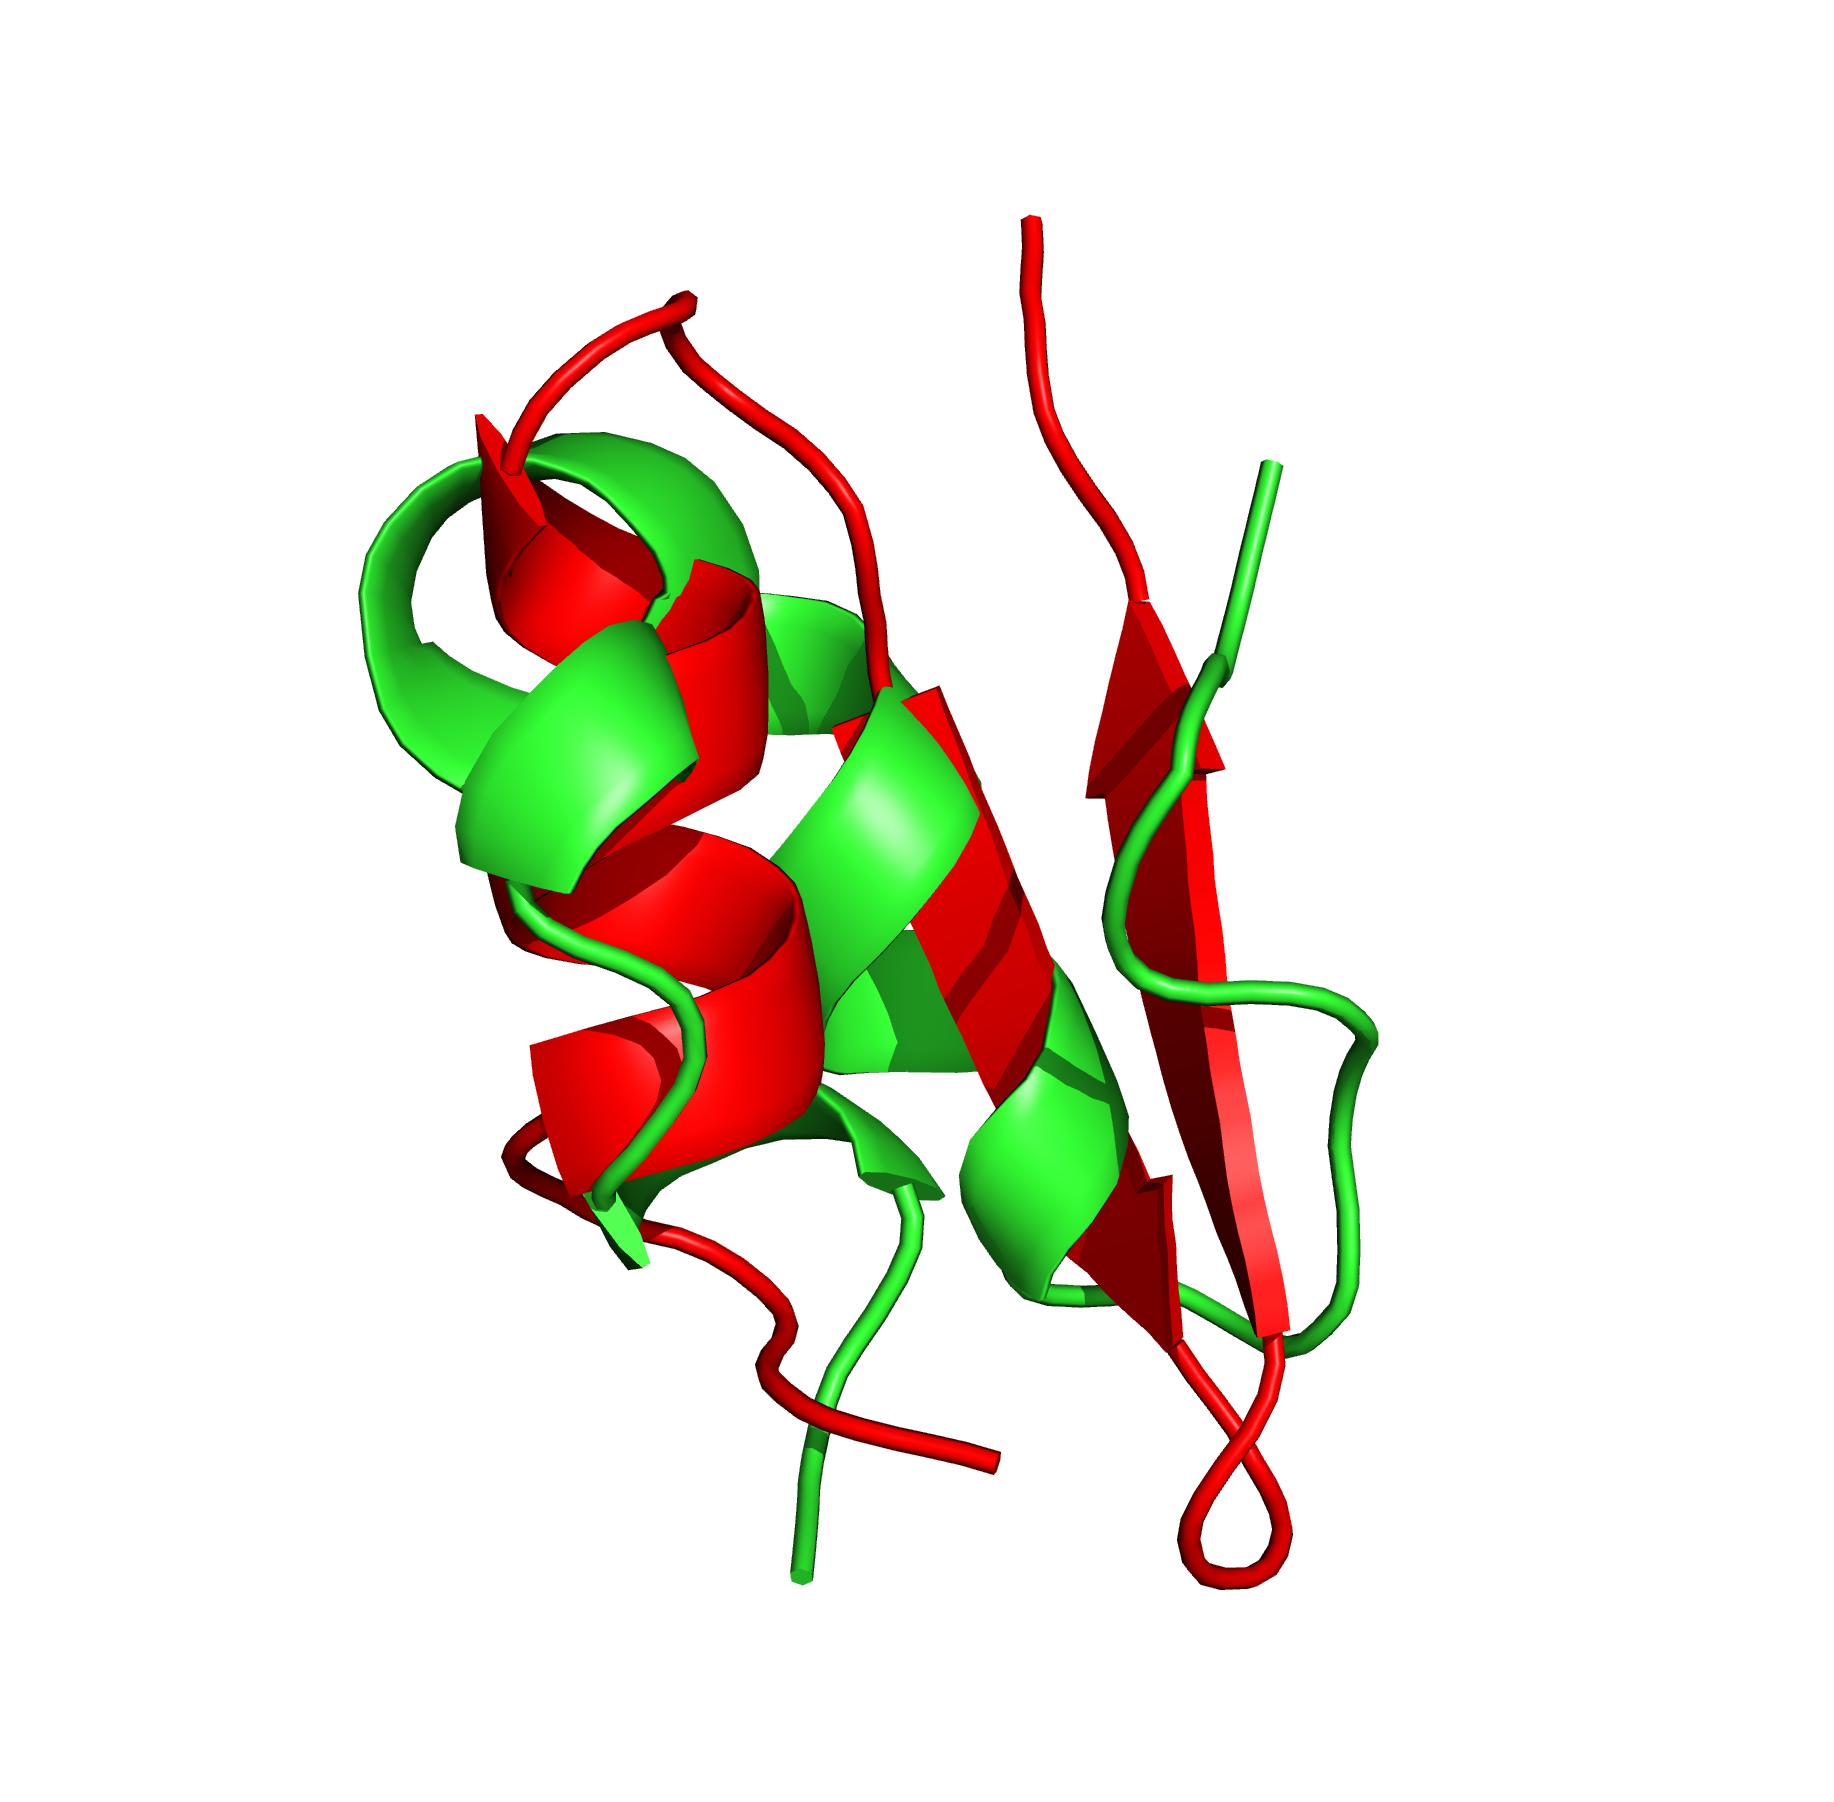
\includegraphics[width=0.9\linewidth]{Figuras/prots/1acw_render.png}
    \caption{1acw (4.45\AA)}
    \label{fig:1acw-conformation}
  \end{subfigure}
%
  \begin{subfigure}{0.24\linewidth}
    \centering
    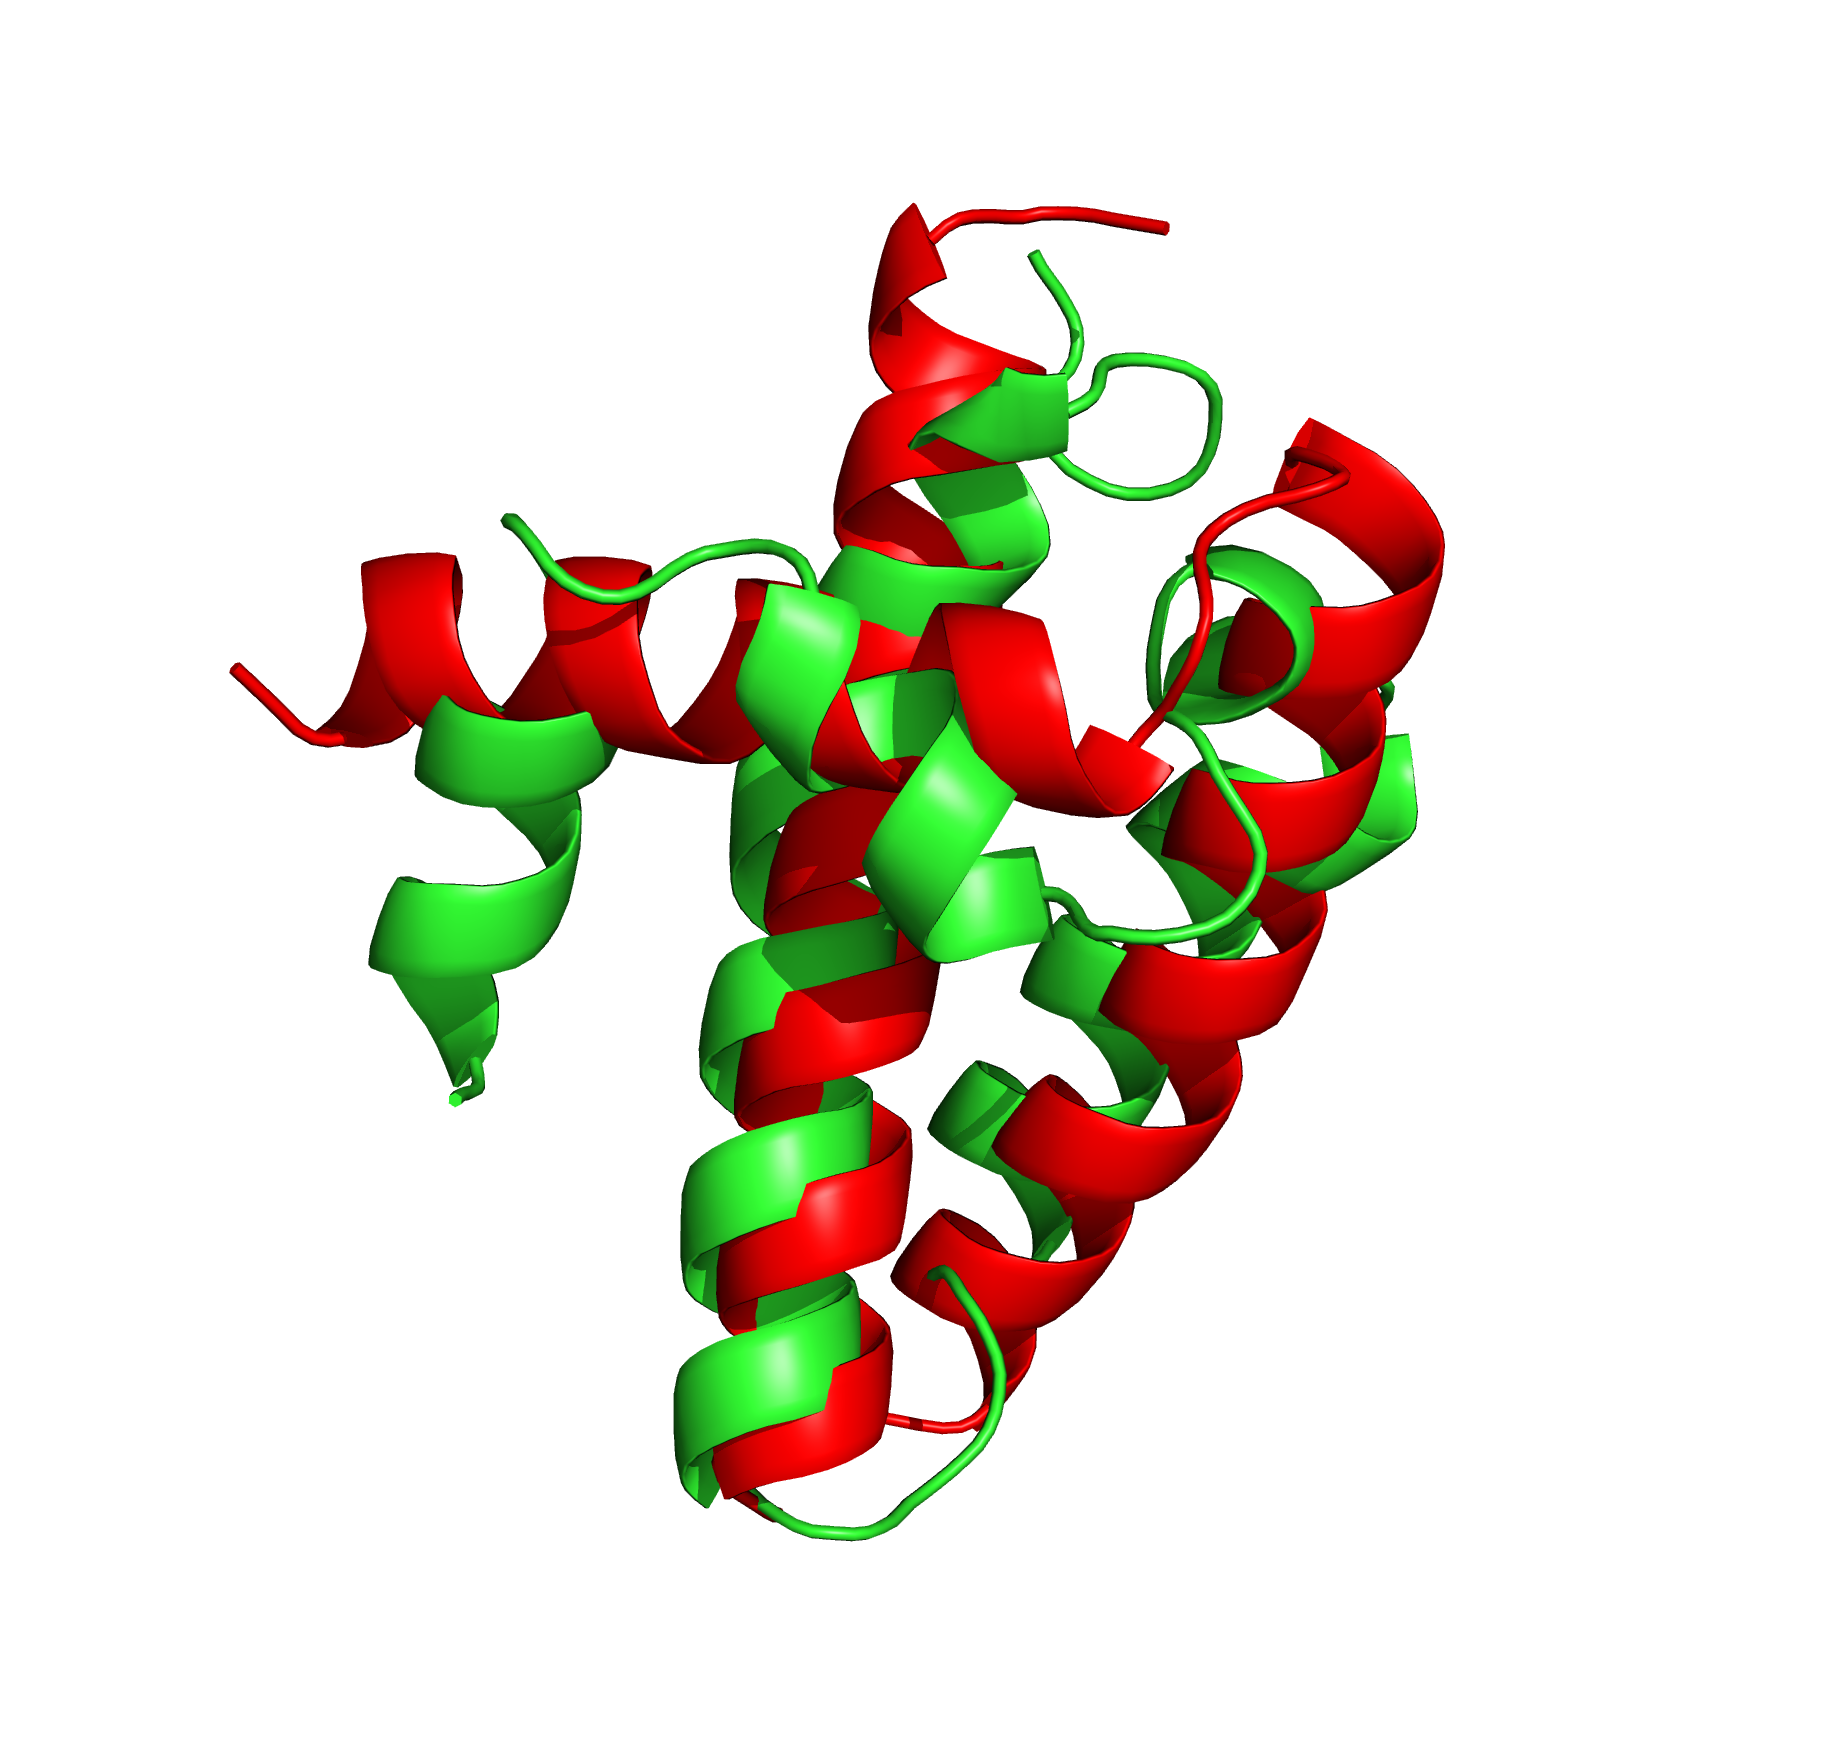
\includegraphics[width=0.9\linewidth]{Figuras/prots/1ail_render.png}
    \caption{1ail (4.26\AA)}
    \label{fig:1ail-conformation}
  \end{subfigure}
%
  \begin{subfigure}{0.24\linewidth}
    \centering
    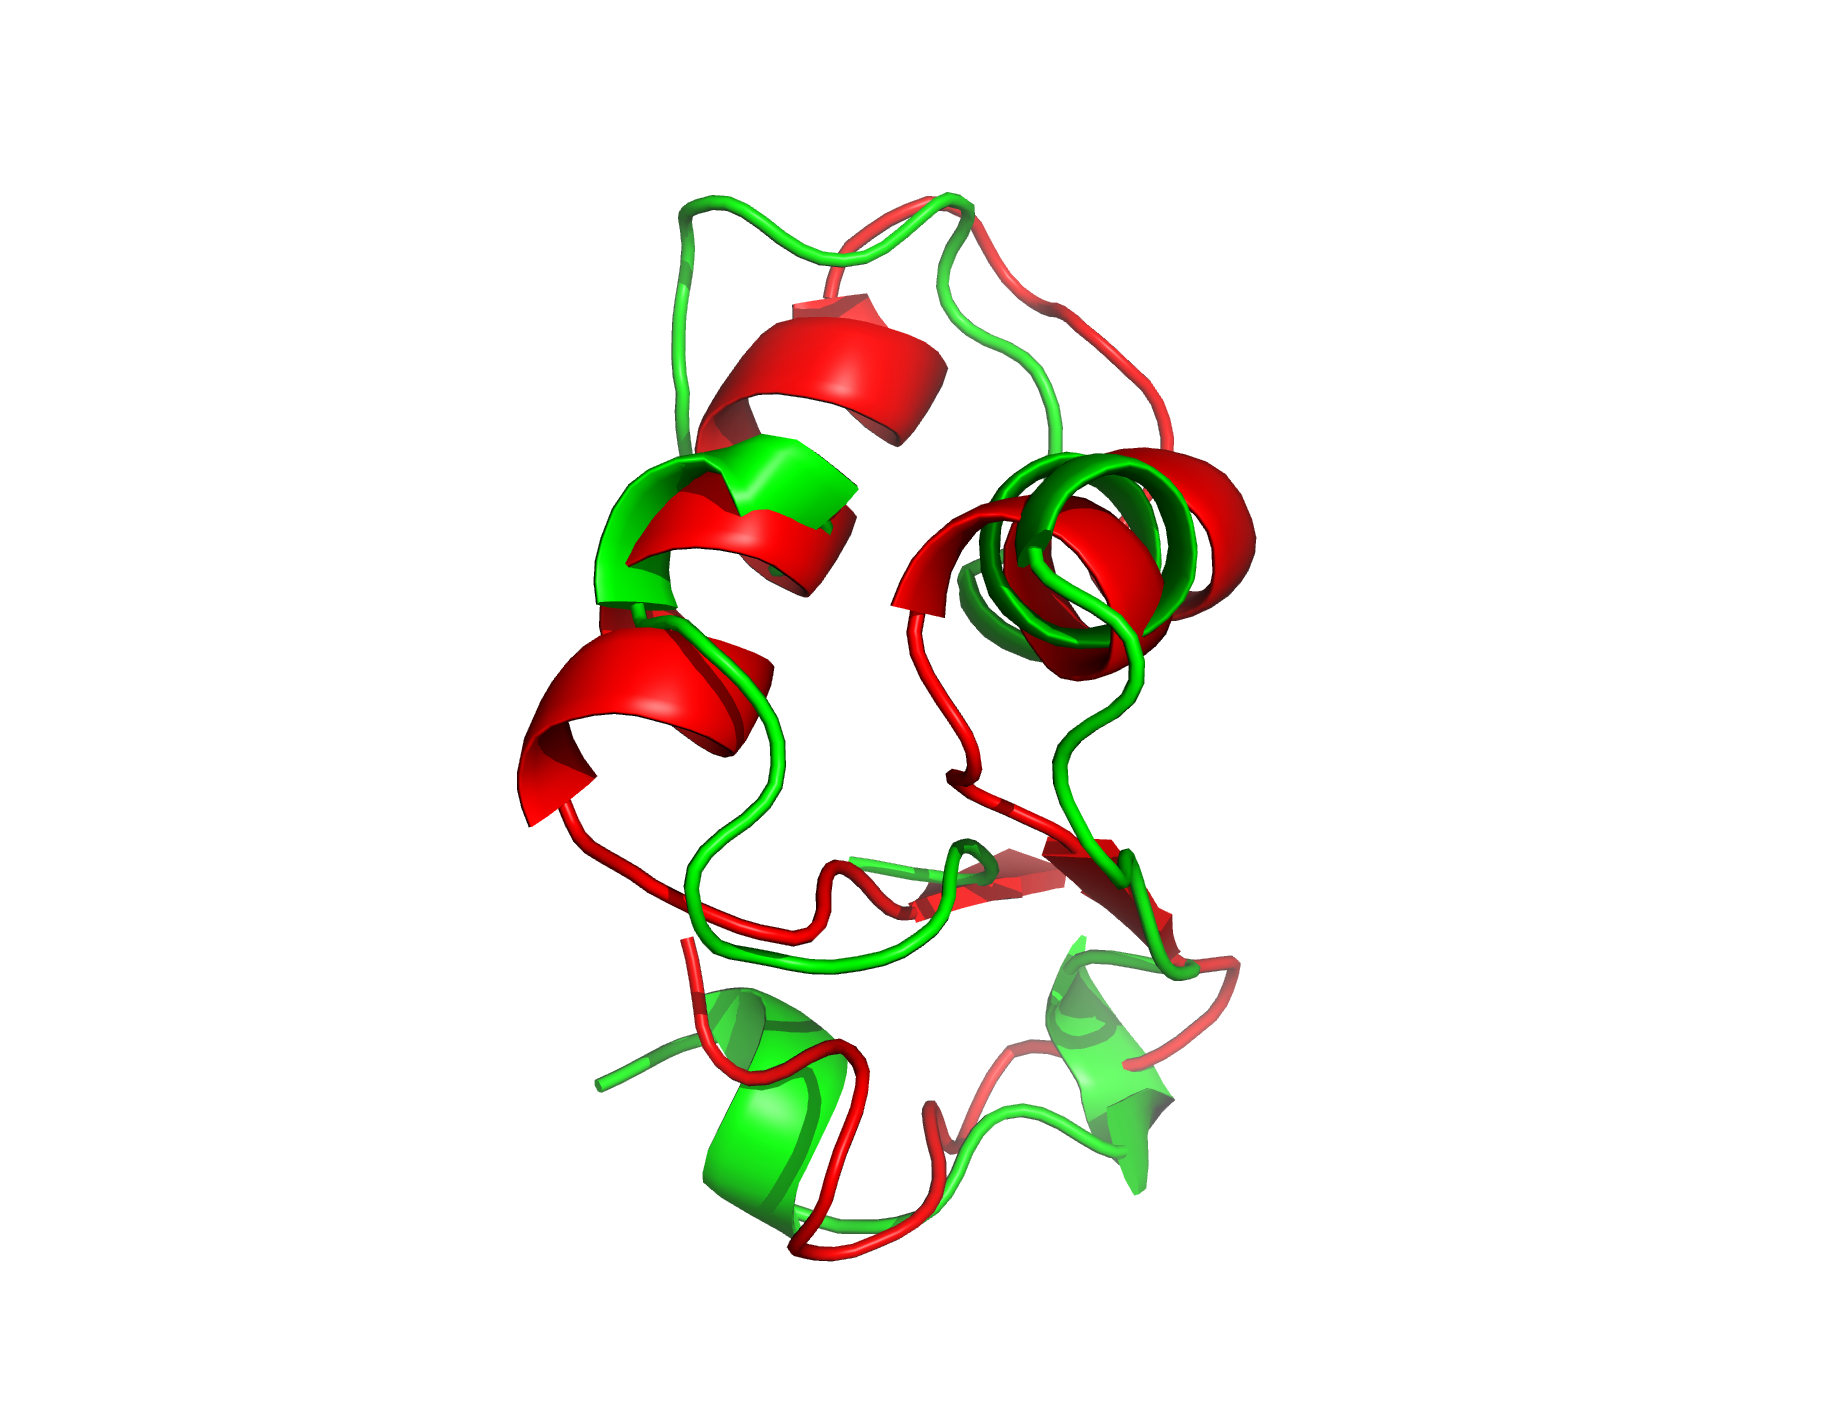
\includegraphics[width=0.9\linewidth]{Figuras/prots/1crn_render.png}
    \caption{1crn (4.18\AA)}
    \label{fig:1crn-conformation}
  \end{subfigure}
%
  \begin{subfigure}{0.24\linewidth}
    \centering
    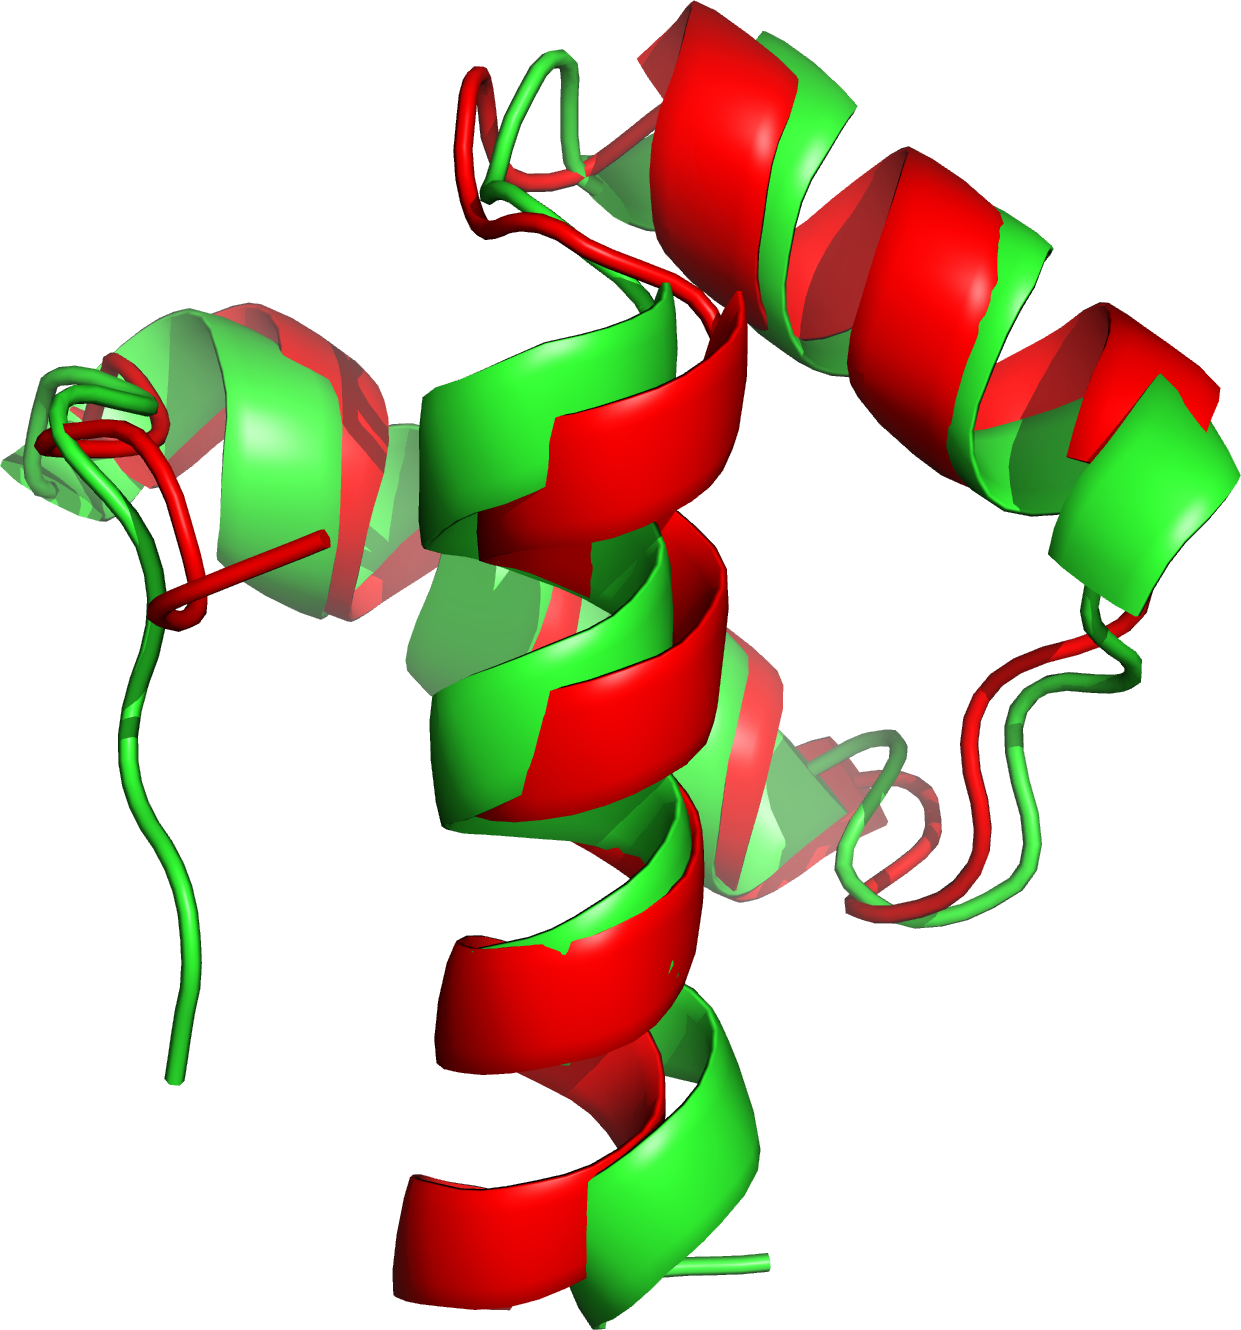
\includegraphics[width=0.9\linewidth]{Figuras/prots/1enh_render.png}
    \caption{1enh (2.65(\AA))}
    \label{fig:1enh-conformation}
  \end{subfigure}
% \end{figure}
% \begin{figure}
  \begin{subfigure}{0.32\linewidth}
    \centering
    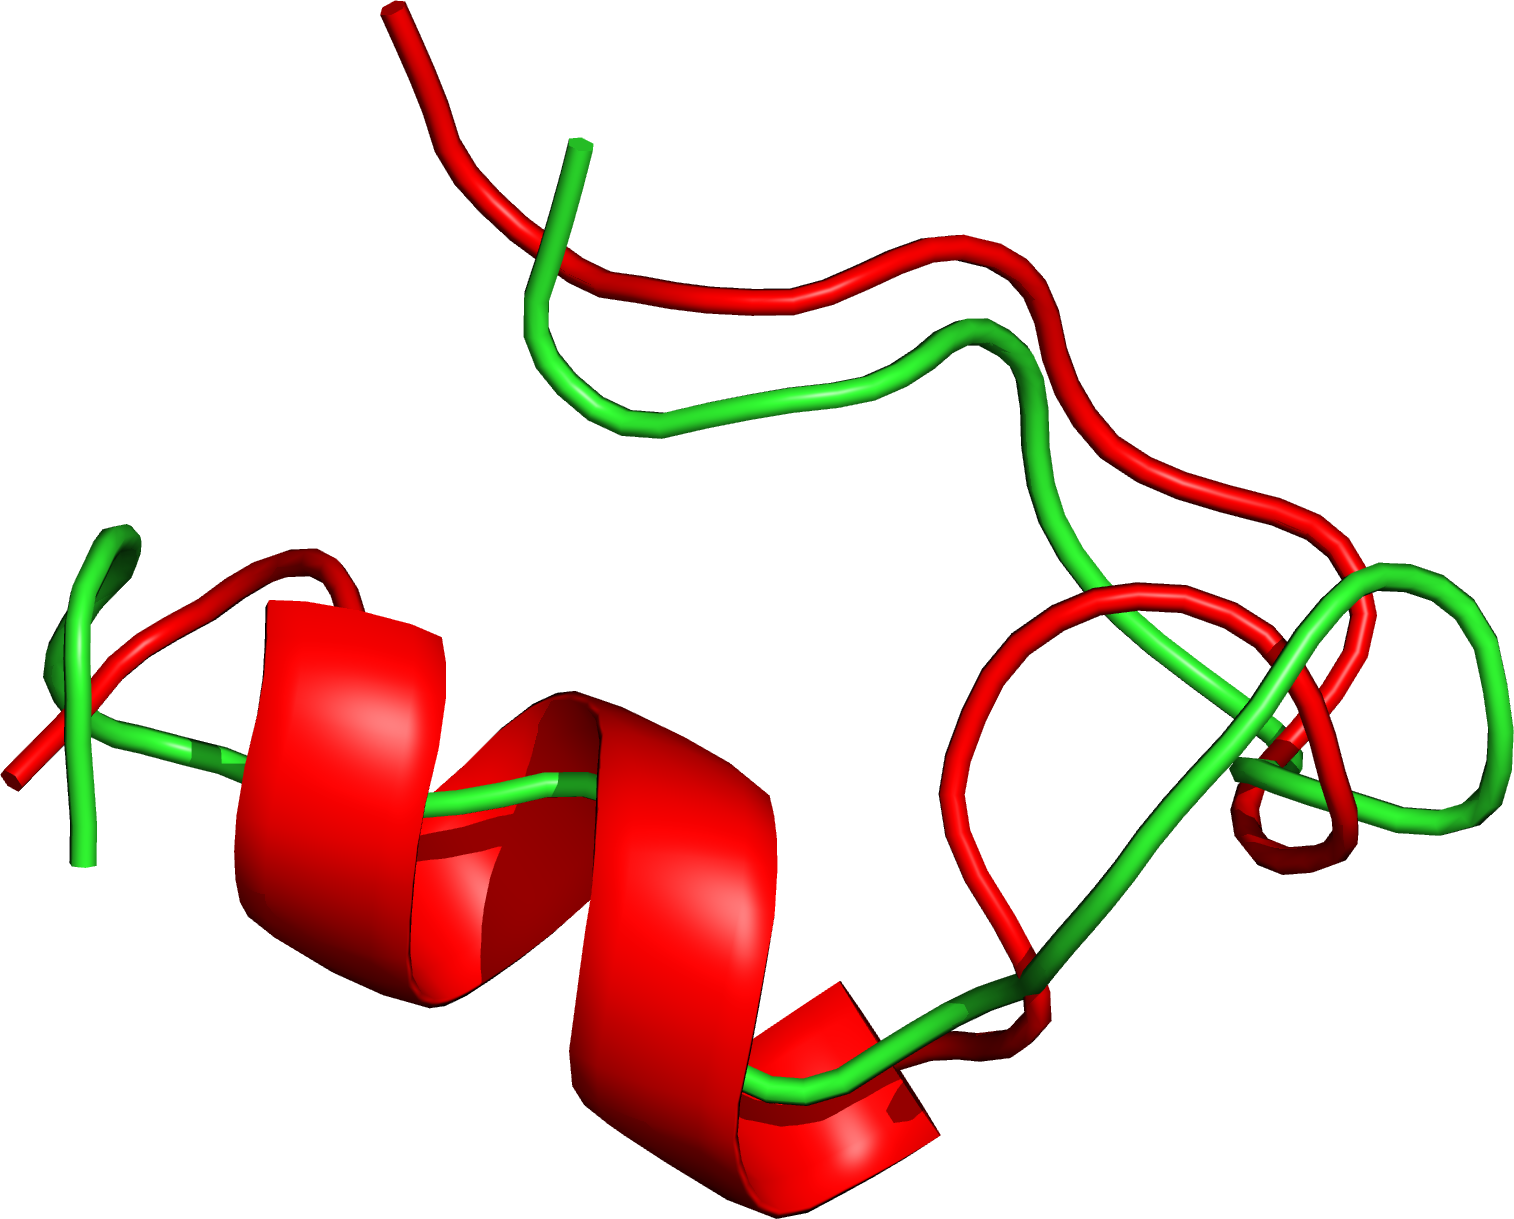
\includegraphics[width=0.9\linewidth]{Figuras/prots/1l2y_render.png}
    \caption{1l2y (3.39\AA)}
    \label{fig:1l2y-conformation}
  \end{subfigure}
%
  \begin{subfigure}{0.32\linewidth}
    \centering
    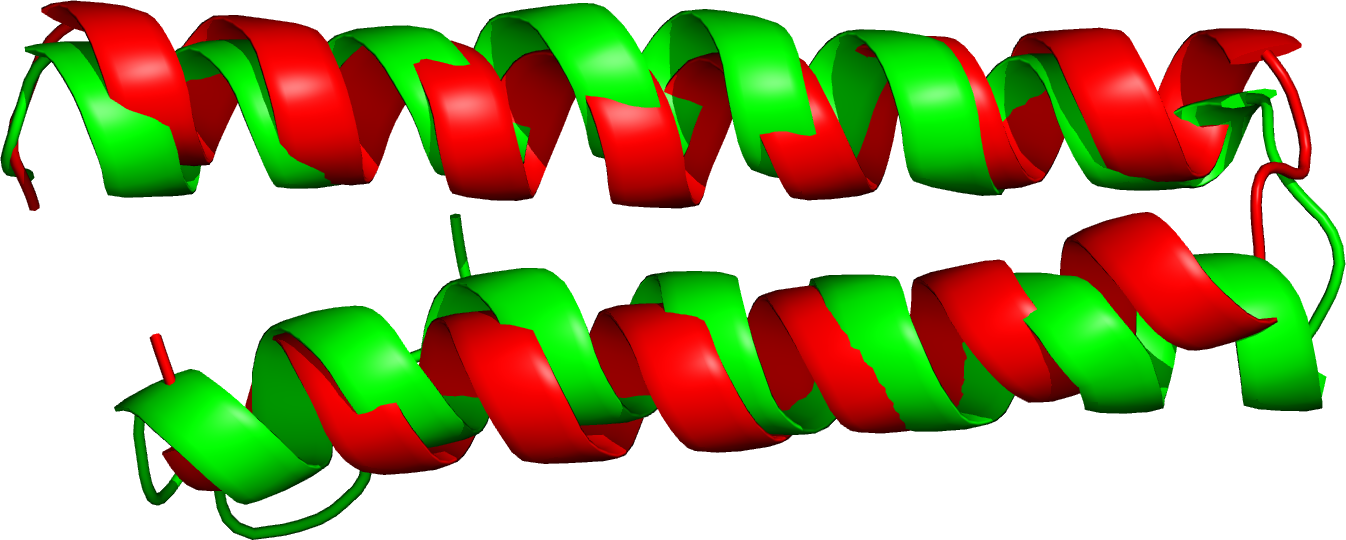
\includegraphics[width=0.9\linewidth]{Figuras/prots/1rop_render.png}
    \caption{1rop (2.18\AA)}
    \label{fig:1rop-conformation}
  \end{subfigure}
%
  \begin{subfigure}{0.32\linewidth}
    \centering
    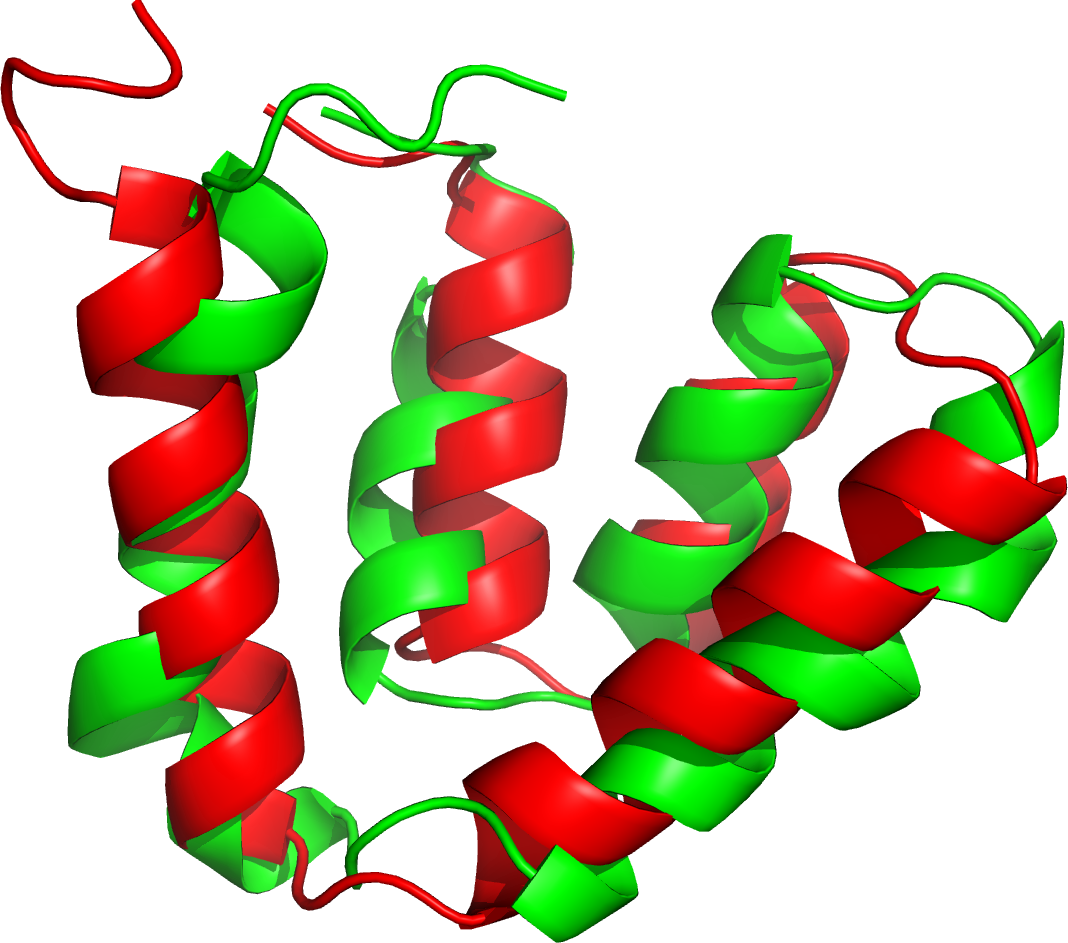
\includegraphics[width=0.9\linewidth]{Figuras/prots/1utg_render.png}
    \caption{1utg (4.41\AA)}
    \label{fig:1utg-conformation}
  \end{subfigure}
% \end{figure}
% \begin{figure}
  \begin{subfigure}{0.32\linewidth}
    \centering
    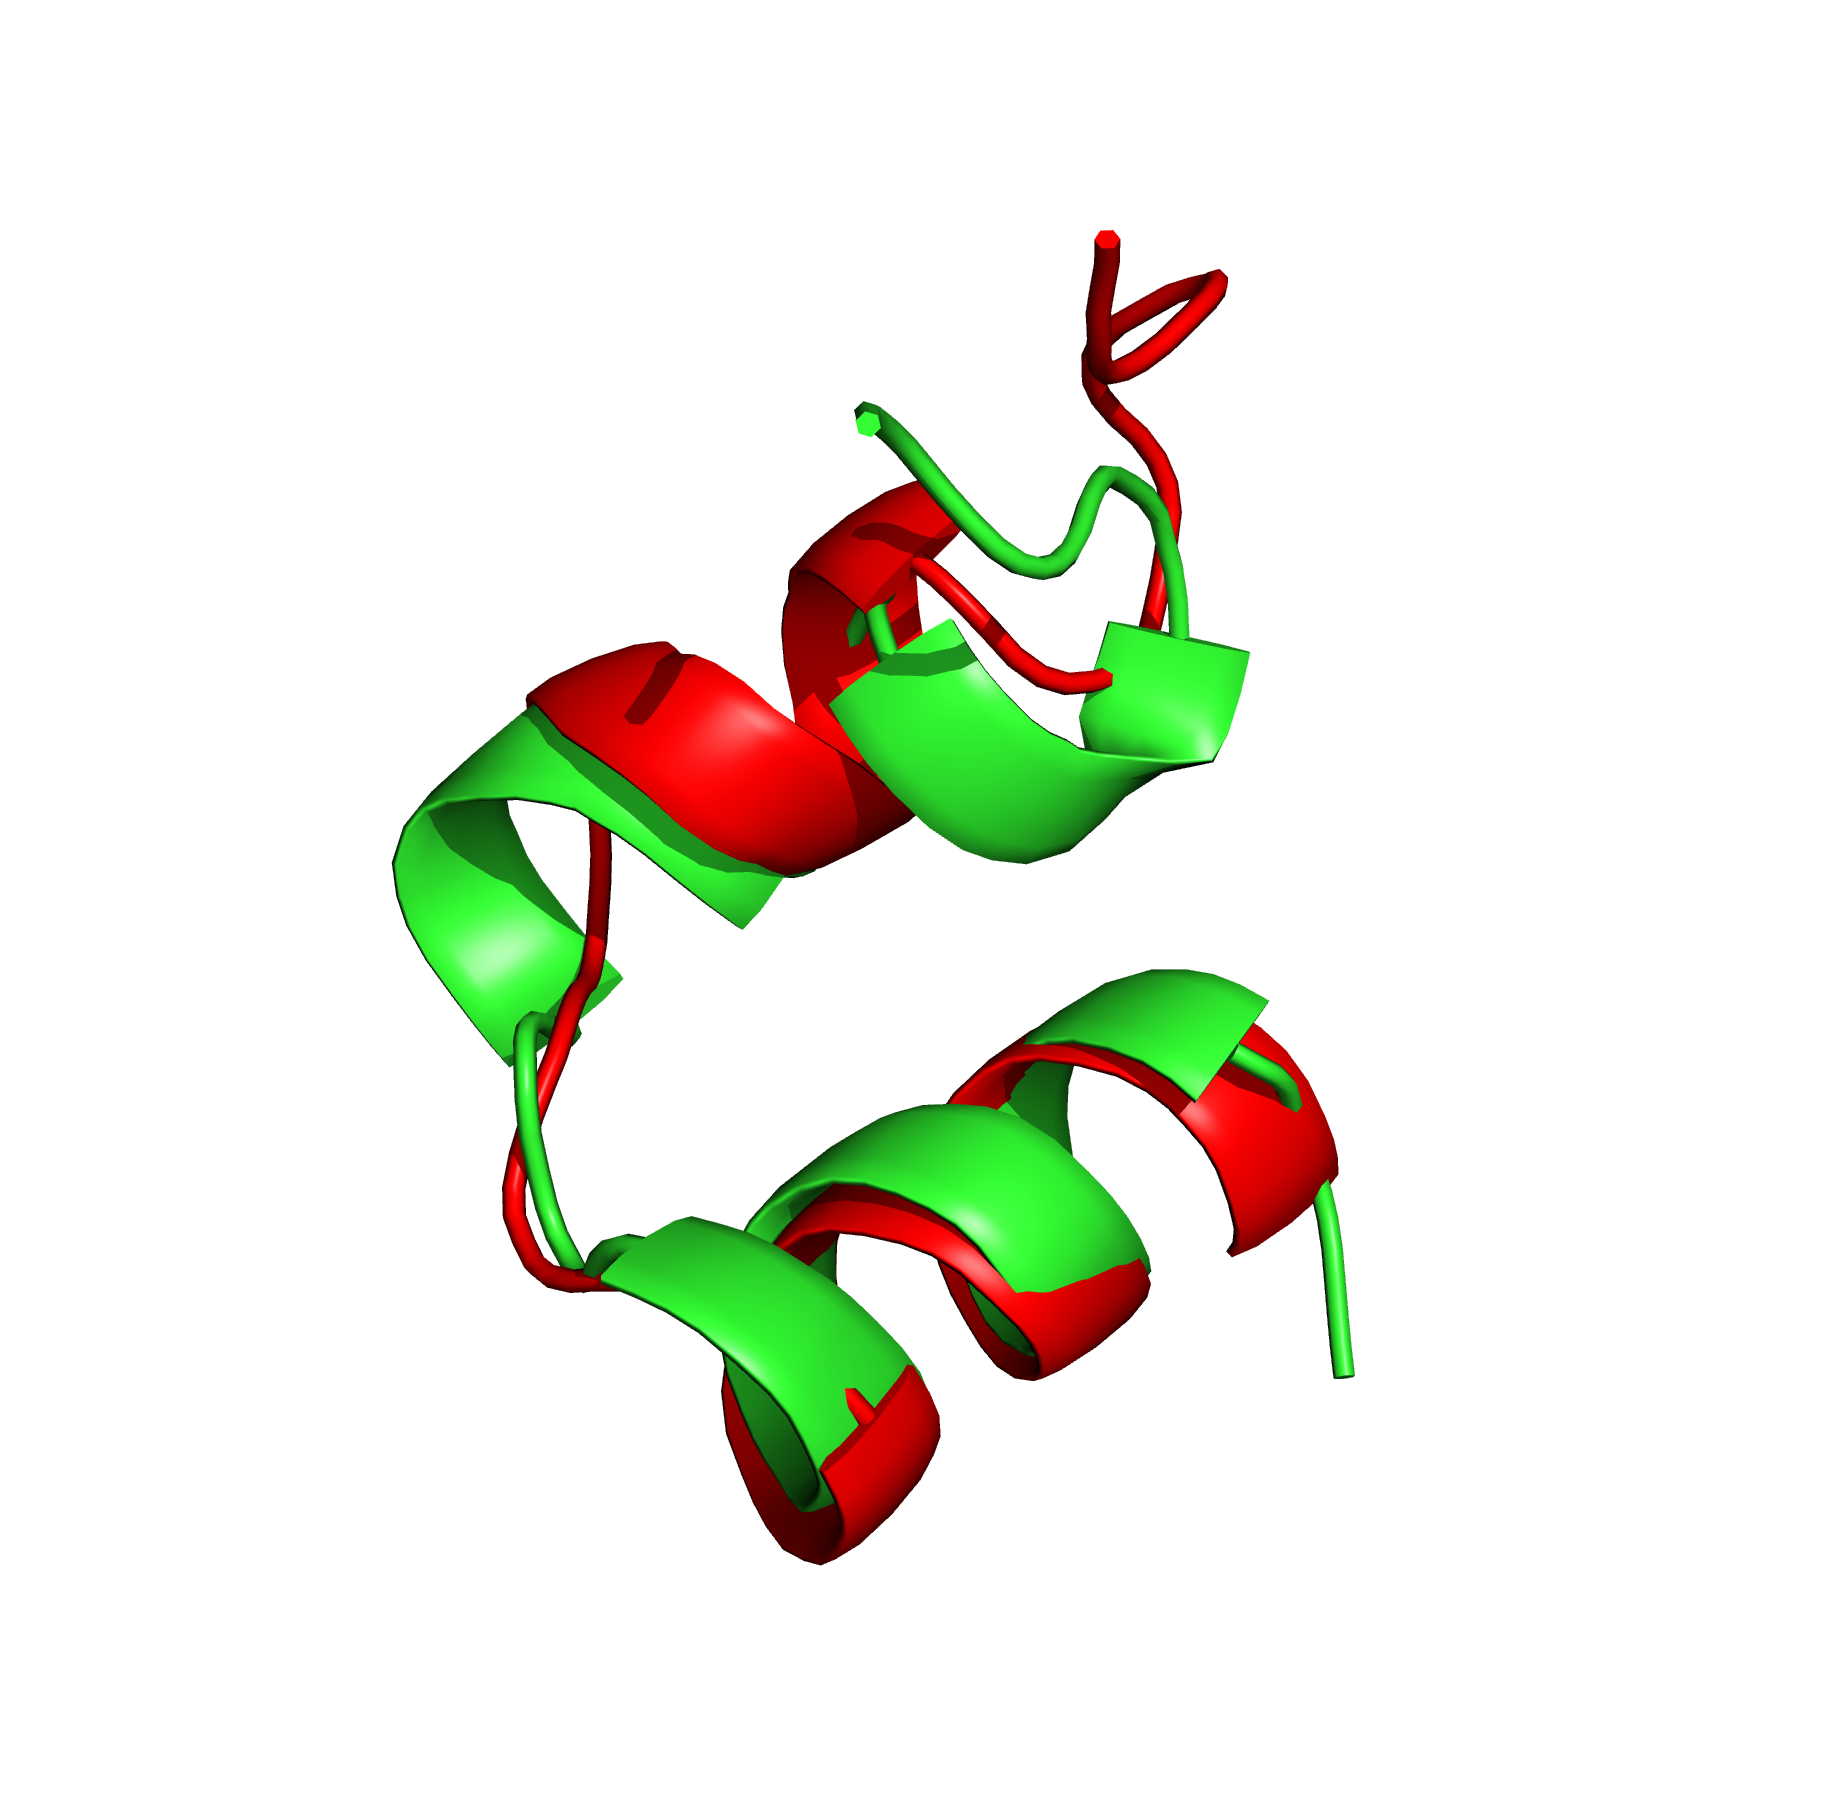
\includegraphics[width=0.9\linewidth]{Figuras/prots/1wqc_render.png}
    \caption{1wqc (2.15\AA)}
    \label{fig:1wqc-conformation}
  \end{subfigure}
%
  \begin{subfigure}{0.32\linewidth}
    \centering
    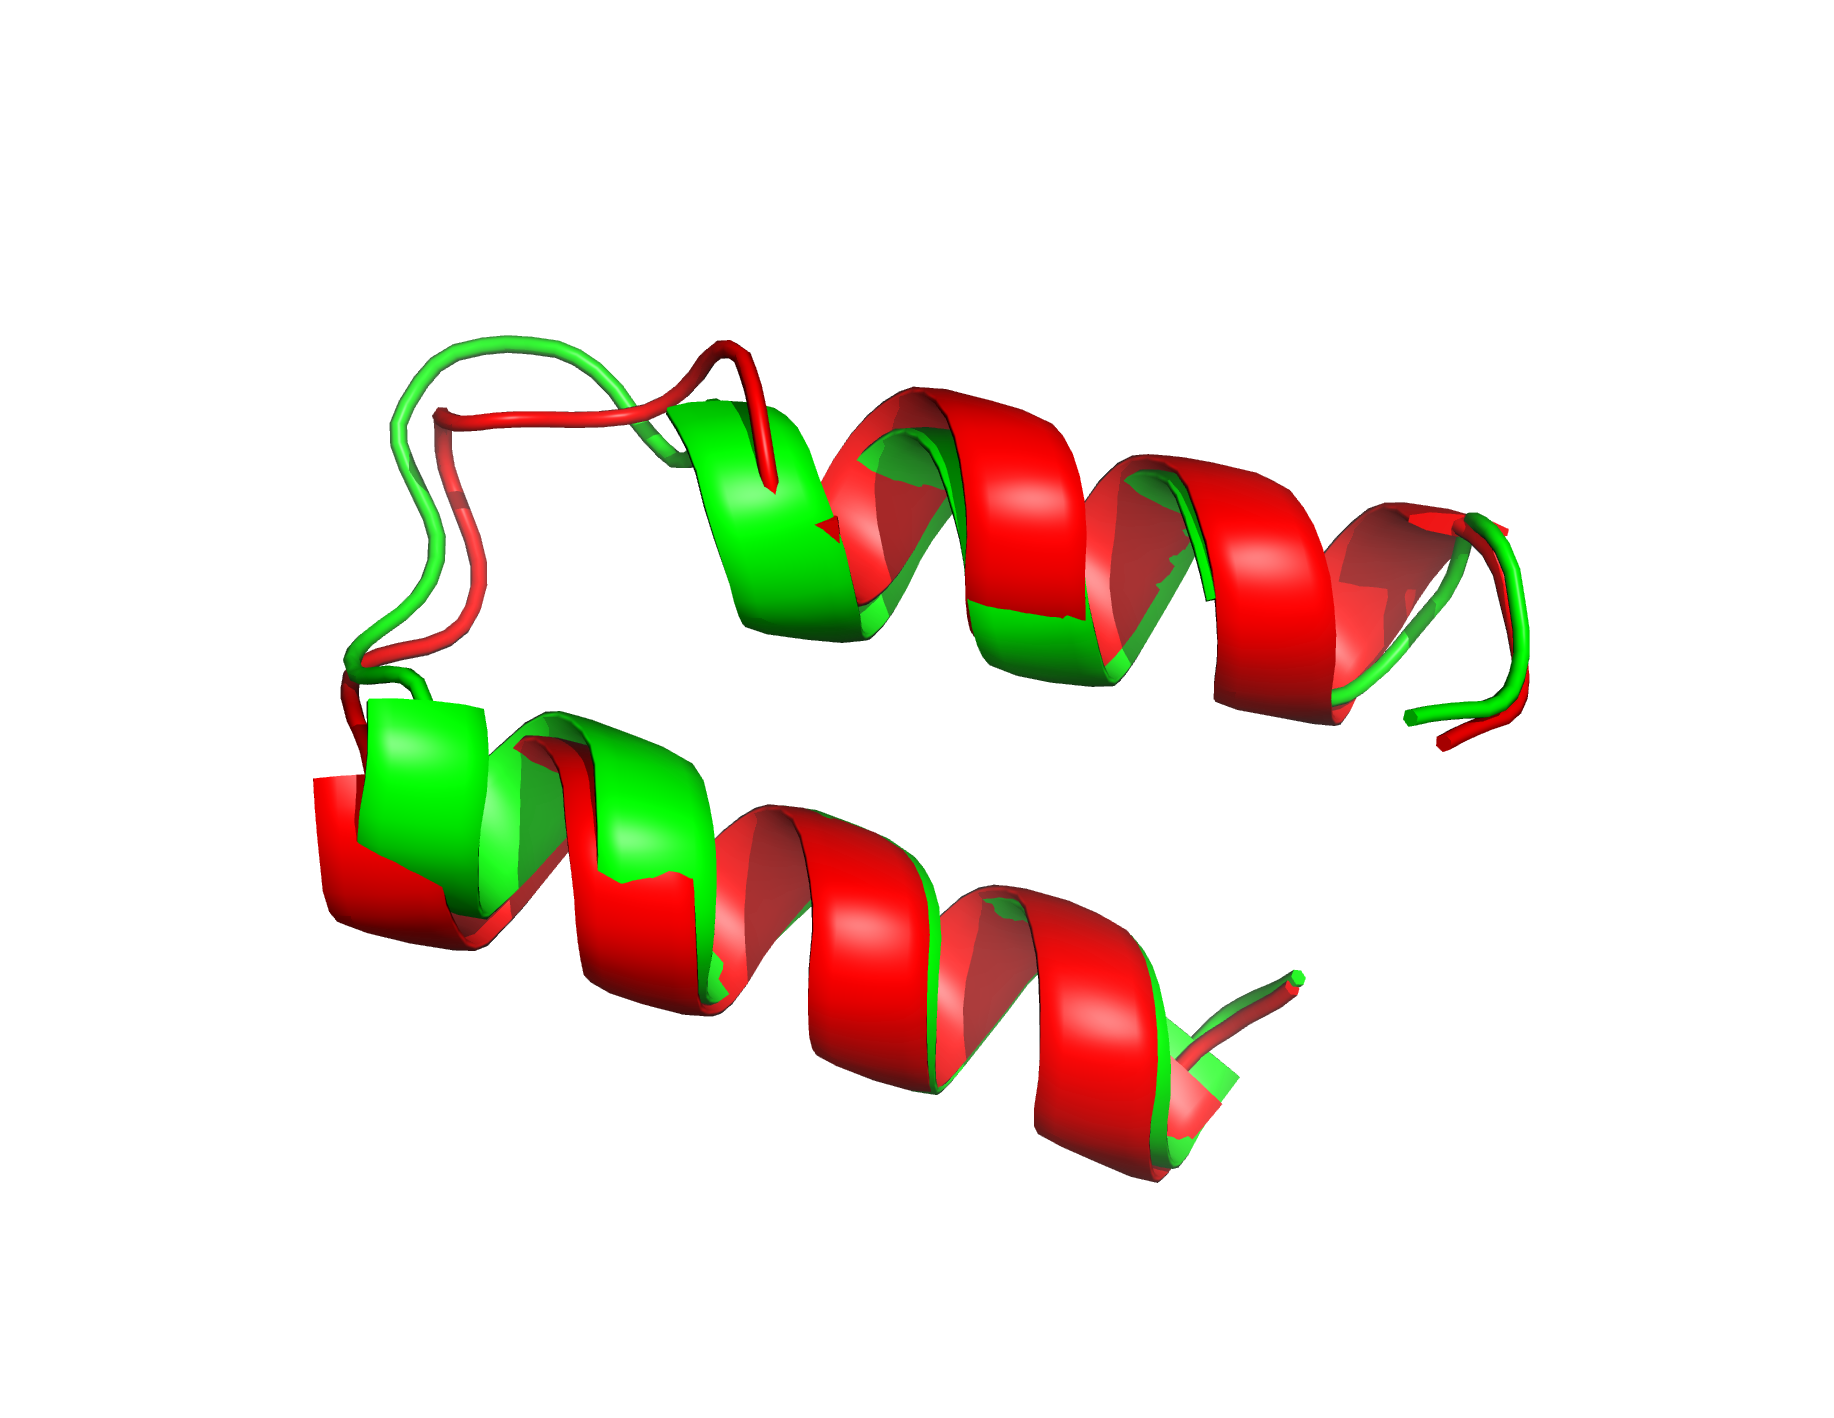
\includegraphics[width=0.9\linewidth]{Figuras/prots/1zdd_render.png}
    \caption{1zdd (1.07\AA)}
    \label{fig:1zdd-conformation}
  \end{subfigure}
%
  \begin{subfigure}{0.32\linewidth}
    \centering
    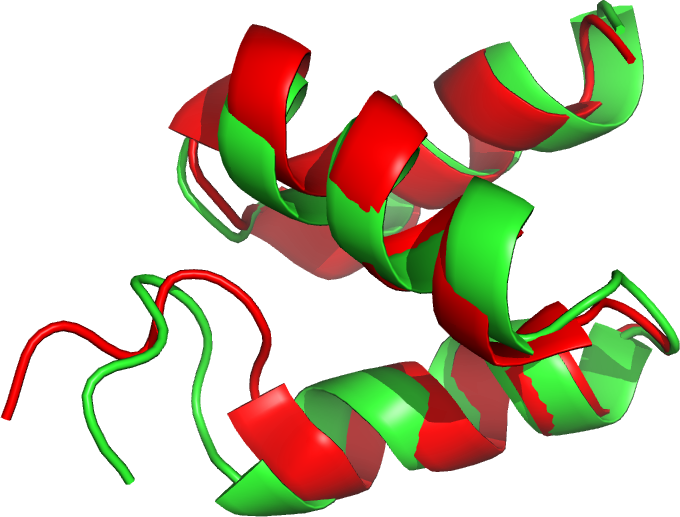
\includegraphics[width=0.9\linewidth]{Figuras/prots/2mr9_render.png}
    \caption{2mr9 (1.66\AA)}
    \label{fig:2mr9-conformation}
  \end{subfigure}
  \caption{The predicted conformations (in green/light gray) compared to the
  native conformation (in red/darker gray). The RMSD between the predicted and
  native conformation is show between parenthesis.}
  \label{fig:all-conformations}
\end{figure}


In Figure~\ref{fig:all-conformations} all conformations from the 10 best
predictions measured by RMSD from PPF-MC are presented. The proteins are presented in
lexicographical order. The predicted conformation is presented in green and the
native conformation is presented in red\footnote{For the readers with a black
and white copy, the predicted conformation is in a light shade of grey, while
the native conformation is in dark grey.}.

Proteins 1enh, 1rop, 1utg, 1wqc, 1zdd and 2mr9 had near native conformations.
%There is very little to comment for these particular predictions.
All the secondary structures are present in their respective regions and the
coil sections closely match their native counterparts.
For protein 1acw,
which had a relatively high RMSD, considering the size of the protein, there are
two main prediction errors. Firstly, the $\beta$-sheets did not form, and, where
should be one, there is an $\alpha$ helix instead. The second error, is that the
$\alpha$ helix is in the wrong place and split. It starts where it should,
however, it only has a single turn. A second helix forms at the eighth residue
and goes on for ten more residues. Both these errors can be traced down to an
error in the Secondary Structure Prediction, which the proposed methods have no
way to avoid. For 1ail, the prediction is mostly correct, however, two helices
are split apart. The first, to the left of the image, and the second, in the
middle helix. These errors were prediction failures that occurred in the proposed methods.
This protein in particular has a correct secondary structure as an starting
point.

On 1crn, a relatively complex protein, has an overall correct fold. The fine
details, however, are lacking. The two helices are mostly missing and the
sheets did not fold. These two errors can be traced down to the secondary
structure prediction used as input. For 1l2y a similar scenario occurs, where
the main source of error is in the data fed to the prediction engine. The
overall shape of the protein was correctly predicted. The helix is completely
missing.

Interestingly, on 4 of the proteins with the biggest visually detectable error
(1acw, 1ail, 1crn and 1l2y)
3 of them (1acw, 1crn and 1l2y) had its source of error outside to the prediction. The proposed method
relies heavily on the predicted secondary structure, and as such, has to deal
with uncertainty. In only a single case the major error in a prediction was
generated during the prediction itself, as occurred on 1ail.

\chapter{Final Considerations and Future Work}
\label{chap:final_considerations}

% Intro to the final considerations
Proteins are macromolecules found in all known living forms and are
considered to be the working horses of the cells. The biological
function of any given protein is directly dependent on its
function, in a way that knowing it is a very valuable information
for several fields of science. The
%Human Genome\footnote{\url{https://www.genome.gov/10001772/all-about-the--human-genome-project-hgp/}}
Human Proteome\footnote{\url{https://hupo.org/human-proteome-project}} project
lead to an exponentially increasing number of sequenced proteins.
However, due to the price and time efforts required to structure
these proteins, a gap quickly formed between the number of sequenced
and the number of structured proteins. This gap now spans more than 3 orders
of magnitude. With that in mind, computer scientists, mathematicians,
physicists, chemists and biologists have been working to accurately
predict the structure of a protein from its primary
sequence and it is known as \textit{ab initio} PSPP.

In light of this, this work proposed two methods, ppf-mc and
ppf-remc, to attempt to solve the problem. The proposed methods make use of the \texttt{score0}, \texttt{score3} and \texttt{scorefxn} energy functions
from Rosetta. The protein was modeled using a full atomic model of the backbone,
manipulated using fragments and torsions angles, as well as side chain centroids.
In later stages of the prediction the model was switch to a full atomic
representation of the protein. The proposed method is capable of outputting
several conformations that are different from each other, this is accomplished
by using a clustering process. This, in turn, would allow for a human expert to
evaluate each of the cluster centroids and choose the best conformation based
on its knowledge and intuition. However, the human input was not explored in this
work. Instead, an oracle was used to replace the human input.

% RMSD and Energy with sade-remc and rosetta
The proposed method were compared against a method from a previous work, SADE-REMC, as
well as rosetta. In a first stage, the two proposed methods were compared
against SADE-REMC using both the RMSD and potential energy.
For both metrics a rigorous set of statistical tests was applied, which identified that
the proposed methods consistently outperformed the competitor both with lower
RMSD and lower potential energies. In a second stage, rosetta, one of the
winners and top competitors at CASP was chosen to be compared against, as a
representative of state-of-the-art. The same statistical framework was applied.
The results indicates that the proposed methods are able to give equal or better
predictions than rosetta for the majority of proteins.

% Convergence
The behavior of the two proposed methods was then inspected and analysed. It was
found that PPF-MC maintained an average pairwise RMSD consistently higher than PPF-REMC.
This lead to more variation in the clusters centroids, which in turn lead to
better predictions. PPF-REMC suffered from premature convergence and stagnation.
The lack of active control of convergence and populational diversity could be
considered as point worth being addressed.
% For one of the targets, this difference was
% of $6\AA$. On the remaining targets this difference varied between $1$ to about
% $2\AA$. One of the properties of PPF-REMC is the capacity of one trajectory to
% effectively copy and replace another, which may lead to faster convergence and
% exploitation. However, as observed, this lead to premature convergence and, in
% some cases, worst results. Meanwhile, PPF-MC was able to cope well with the
% clustering phase of the resulting conformation, thanks to its high diversity.
% Nevertheless, during this analysis, it was observed by tracking the best energy
% and average energy, that FFI was worsening the convergence for some methods.
% Due to its nature, for 1enh and 2mr9 it was observed that despite the greedy
% selection of conformation FFI was making the energy increase faster than the
% optimizer could keep up.

% MC vs REMC
With data from the convergence of the two proposed methods and statistical
analysis, a direct comparison of both methods was realized. When considering
only the RMSD there was statistical significance only for one protein, 1rop.
However, when considering the potential energy, PPF-MC had statistically
significant better energies for $5$ out of $10$ protein targets. Moreover,
despite the statistical significance of RMSD for only one target, PPF-MC had
the conformations with the best RMSD for $5$ targets. This, plus the fact that
PPF-MC has more diversity combined with the conformational clustering leads to
the conclusion that PPF-MC is the superior method. 

% Repacking Impact
% An analysis to assess the impact of repacking was also realized. The goals were
% twofold. Firstly, there was the interest in verifying that the repacking process
% was not misleading or interfering in the results. Secondly, just the plain
% documentation of how much repacking impacted the process was desirable. This
% information was not found in the literature.
Based on an analysis of repacking, it was found that
the repacking process had a small negative impact in the energies of the
proposed methods. Before repacking, both proposed methods had more results that
were better than rosetta with statistical significance. After applying repacking,
this number decreased. The mean change in RMSD was also documented. It was found
to be very low. In most cases it was lower than $0.5\AA$ on average.

% Processing time and function evaluations
% The processing time was also documented. There was no significant difference
% between the proposed methods. The main goal of analysing the processing time was
% to give a time-frame of how long it took for the prediction to be made. Along
% with this, an analysis of the total of function evaluations spent also was
% presented. The methods, on average, take less than 20 minutes to run, even for
% the bigger proteins. For the smaller proteins, the targets can be predicted in
% 10 minutes or less.

% The optimization phase of the proposed method uses 1 million of function
% evaluations, using the \texttt{score3} energy function. This is were the bulk
% of processing happen. Before this phase, the \texttt{score0} energy function
% can spend up to 10 thousand function evaluations for generating the initial
% population. Finally, in the post processing phase, the Hooke-Jeeves search
% procedure spends on average 20 thousand function evaluations. A value relatively
% small compared to the budged from the optimization phase. Nevertheless, this
% data is made available in order to give a solid ground for future comparisons
% with the presented methods.

% Literature comparison
To be able to compare the proposed methods against the literature, a literature
review was realized, which selected the 10 most common proteins.
Based on this, it was found that the proposed methods are
competitive with several methods in the literature. For two targets 1wqc and
2mr9 the proposed methods were able to overpass the best result found in the
literature. For 1rop and 1crn, the two proteins used more often in the
literature, one of the proposed methods were able to get the second best
prediction. The same occurred for 1enh. For the remaining targets the proposed
methods achieved results that were often close to the best results available.

% GDT-TS and TMScore
A second analysis of prediction error was realized using GDT-TS and TM-Score,
which provided further insights, complementary to RMSD. Firstly, it was observed
that GDT-TS appears to be more strict about the results than RMSD. Furthermore,
TM-Score appears to be even stricter. Another key-point observed, is that the
three metrics does not always agree, where they gave values significantly
apart. Nevertheless, studying the GDT-TS and TM-Score gave the insights that
the prediction could be improved even further for several of the proteins which
judging just by RMSD alone were considered near native conformations. In the end,
the raw data from these observations was made available in order to allow for
future works to compare against ours using rigorous statistical methods.

% Visual Analysis
A visual analysis was utilized to try and identify what the main prediction
errors were. Four proteins were detected as having major errors. From these,
three had its errors tracked down to the predicted secondary structure, which is
and input of the proposed methods. As such, the predictions were made using
incorrect data, leading to a sub par performance. The dependency on
uncertain data is potentially one of the major weak-spots of the proposed methods.
Nevertheless, for the majority of the predictions correct predictions were made.

\section{Future Works}\label{sec:future_works}

% Secondary Structure Prediction
A future research direction
would be to employ more than one predictor, in a way that if one is wrong,
there is a chance that the other is not. It is also possible to research in the
direction of making the Tertiary Structure Prediction either less dependent on
the Secondary Structure Prediction or making it more resilient to faulty
information.

% Better frags
The use of better generated fragments is also a research direction, since a big
portion of the conformation sampling method is dependent on it. A fragment
library of poor quality will lead to a poor prediction.
% More hybridization
The further hybridization with methods can also be considered. One possible
direction is the inclusion on gradient descent methods to quickly find nearby
areas of low energy.
% Diversity
%Another weak point of this work is that there is no passive or active method of
%controlling the diversity of the population.
As show in works~\citeonline{narloch2016diversification,simoncini2017balancing},
actively or passively acting on populational diversity can lead to
better predictions. As such, managing populations diversity might further
extend the potential of using conformational clustering.

% Better conformation sampling
A recent trend worth exploring is the focusing the search on loops and coil
regions of the proteins. These areas usually have a lower acceptance rate of
perturbation due to the high impact they have on the overall conformation.  In
contrast, $\alpha$-helices are relatively stable and have a much higher
acceptance rate while having a low impact in the overall structure.

% Add restarts
Running a method for too long will most likely given diminishing returns, as
the diversity decreases. One way to give better predictions is to periodically
reset parts of the population or the full population if stagnation occurs. This
can allow for the method to run longer and possibly lead to better predictions.
In particular, partial population re-initialization can allows for old information
to contribute to the newer generated individuals.

% LS for SaDE
The proposed methods applied Hooke-Jeeves pattern search as one of the last steps.
However, on direction would be to use Hooke-Jeeves, or other local search
procedure as an operator for SaDE. This would allow for the method to quickly
find local regions of good potential energy. However, this could also lead to
premature convergence, and as such, it must have a counter acting way of
preventing the population from getting stuck. Further, due to the nature of
SaDE, it is possible that the local search operators perform too well at the
start, making SaDE heavily prefer it. Then, at latter stages, they will
have diminishing returns. However, SaDE will keep heavily applying the
same operators over and over again. Therefore, it might be required for another
strategy to be utilized to control which operator is applied.


\bookmarksetup{startatroot}

\postextual

\bibliography{references}

\begin{apendicesenv}
  \chapter{Graphical Representation of the Predicted Conformations}\label{appendix:visual}

\begin{figure}[ht]
    \centering
    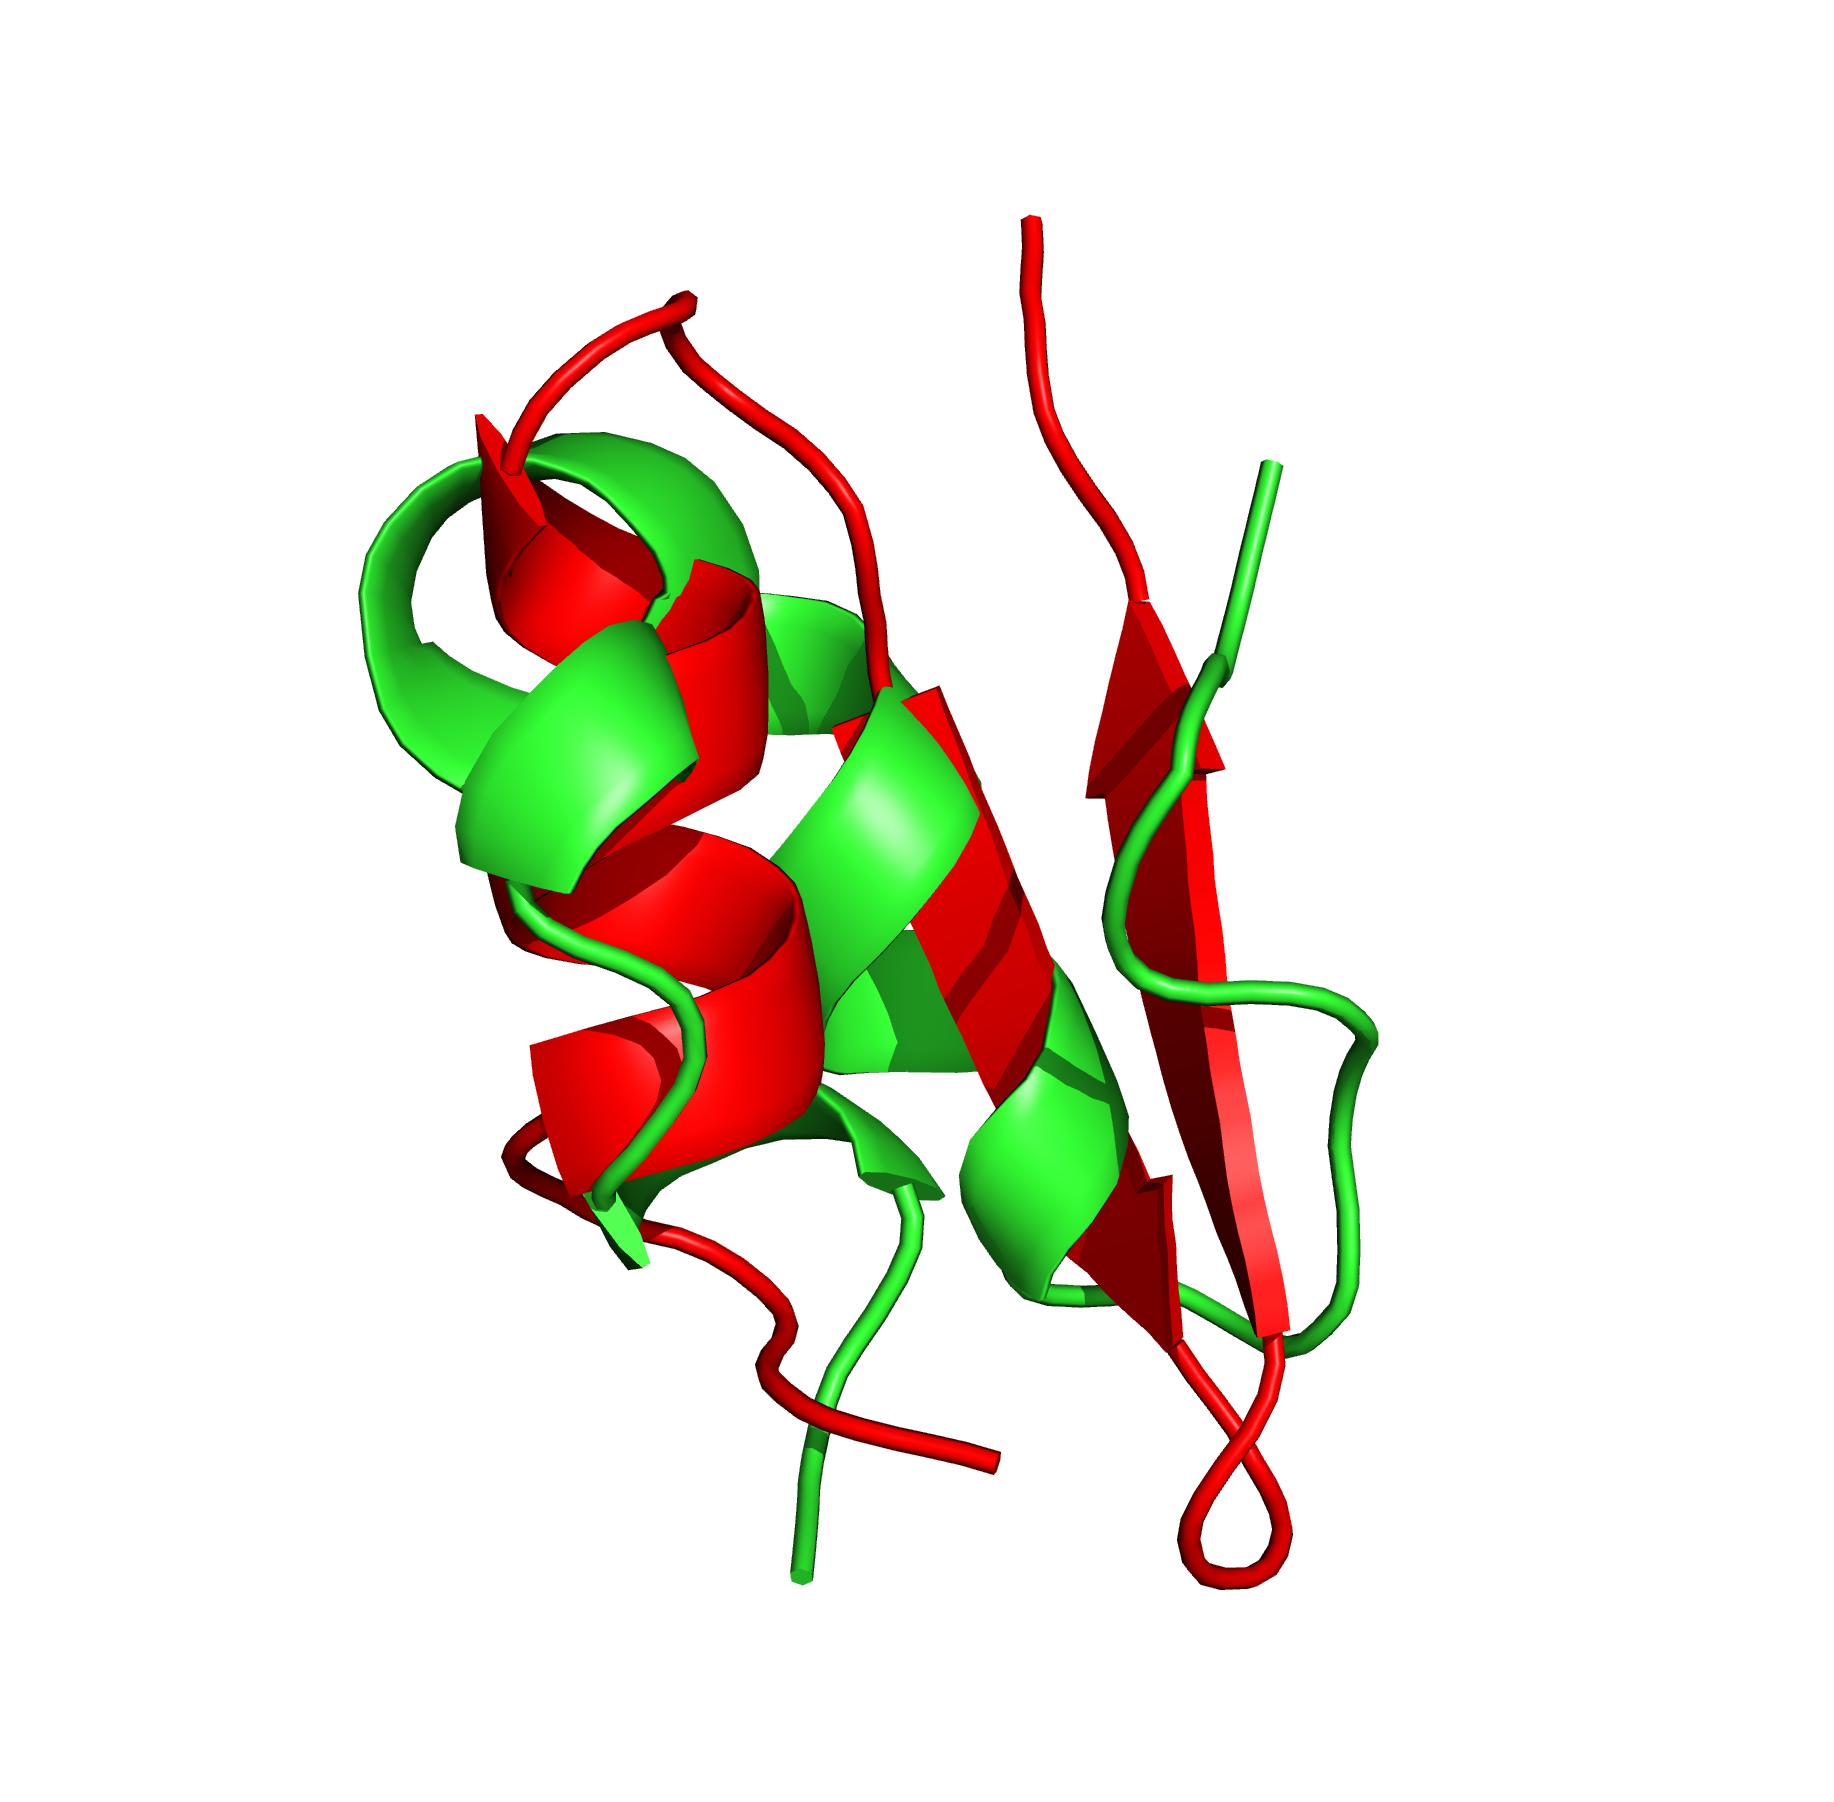
\includegraphics[width=0.9\linewidth]{Figuras/prots/1acw_render.png}
    \caption{Predicted Conformation of 1acw (green, light) over the Native Conformation}
    \label{fig:1acw-visual}
\end{figure}

\begin{figure}[ht]
    \centering
    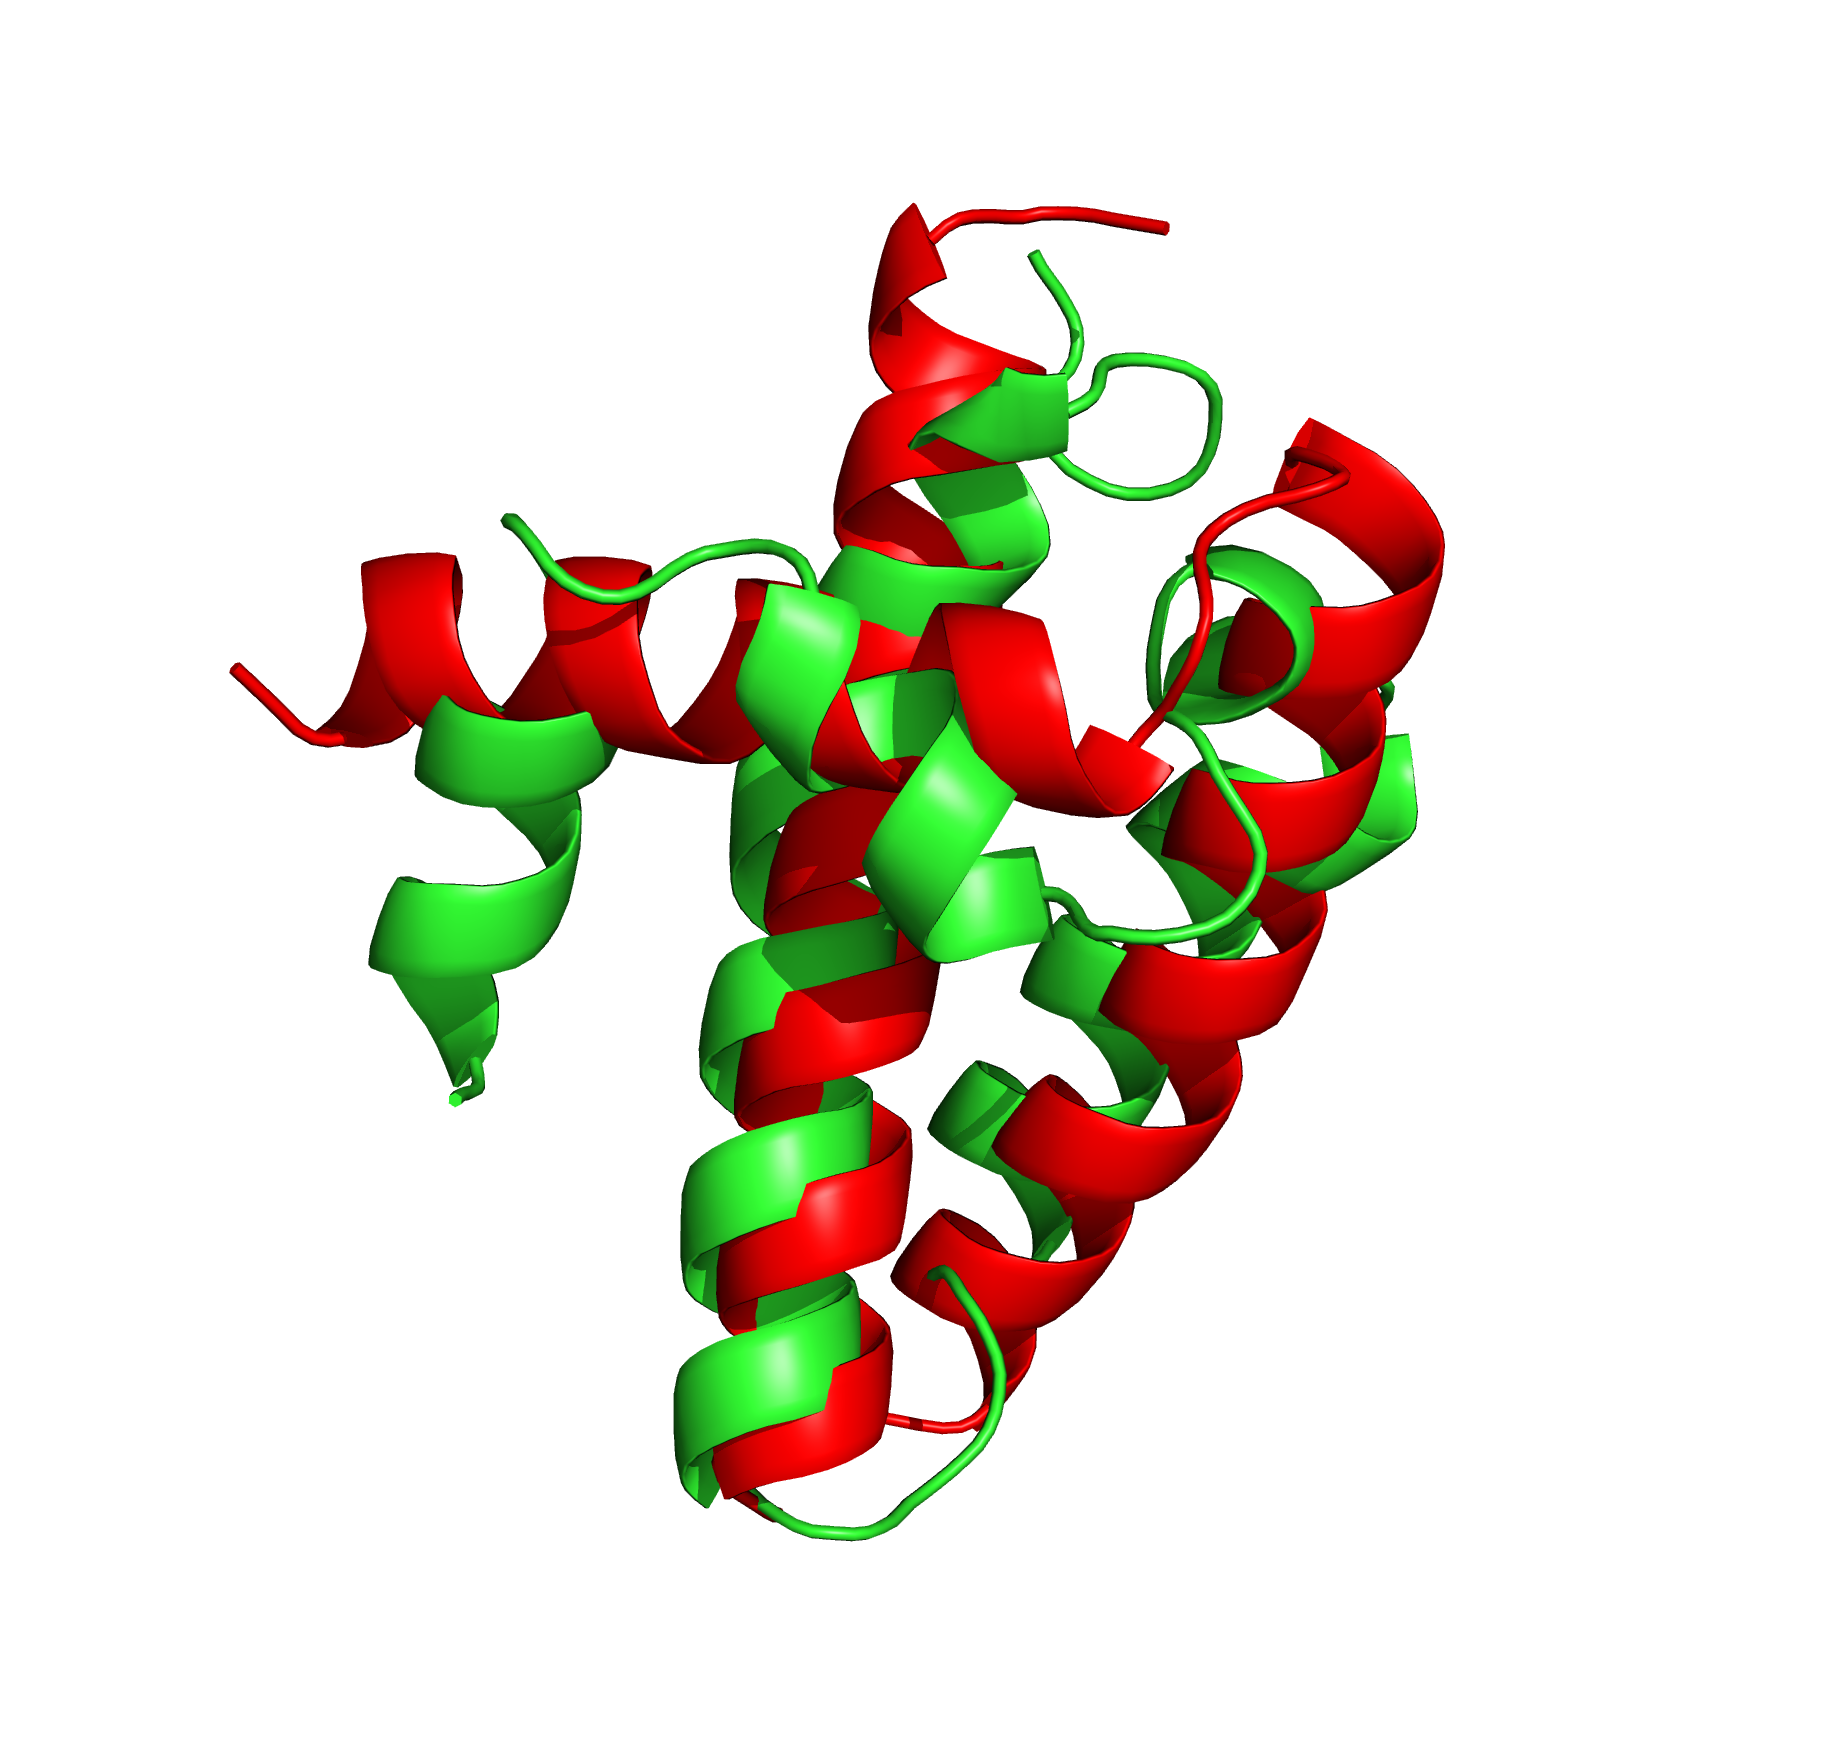
\includegraphics[width=0.9\linewidth]{Figuras/prots/1ail_render.png}
    \caption{Predicted Conformation of 1ail (green, light) over the Native Conformation}
    \label{fig:1ail-visual}
\end{figure}

\begin{figure}[ht]
    \centering
    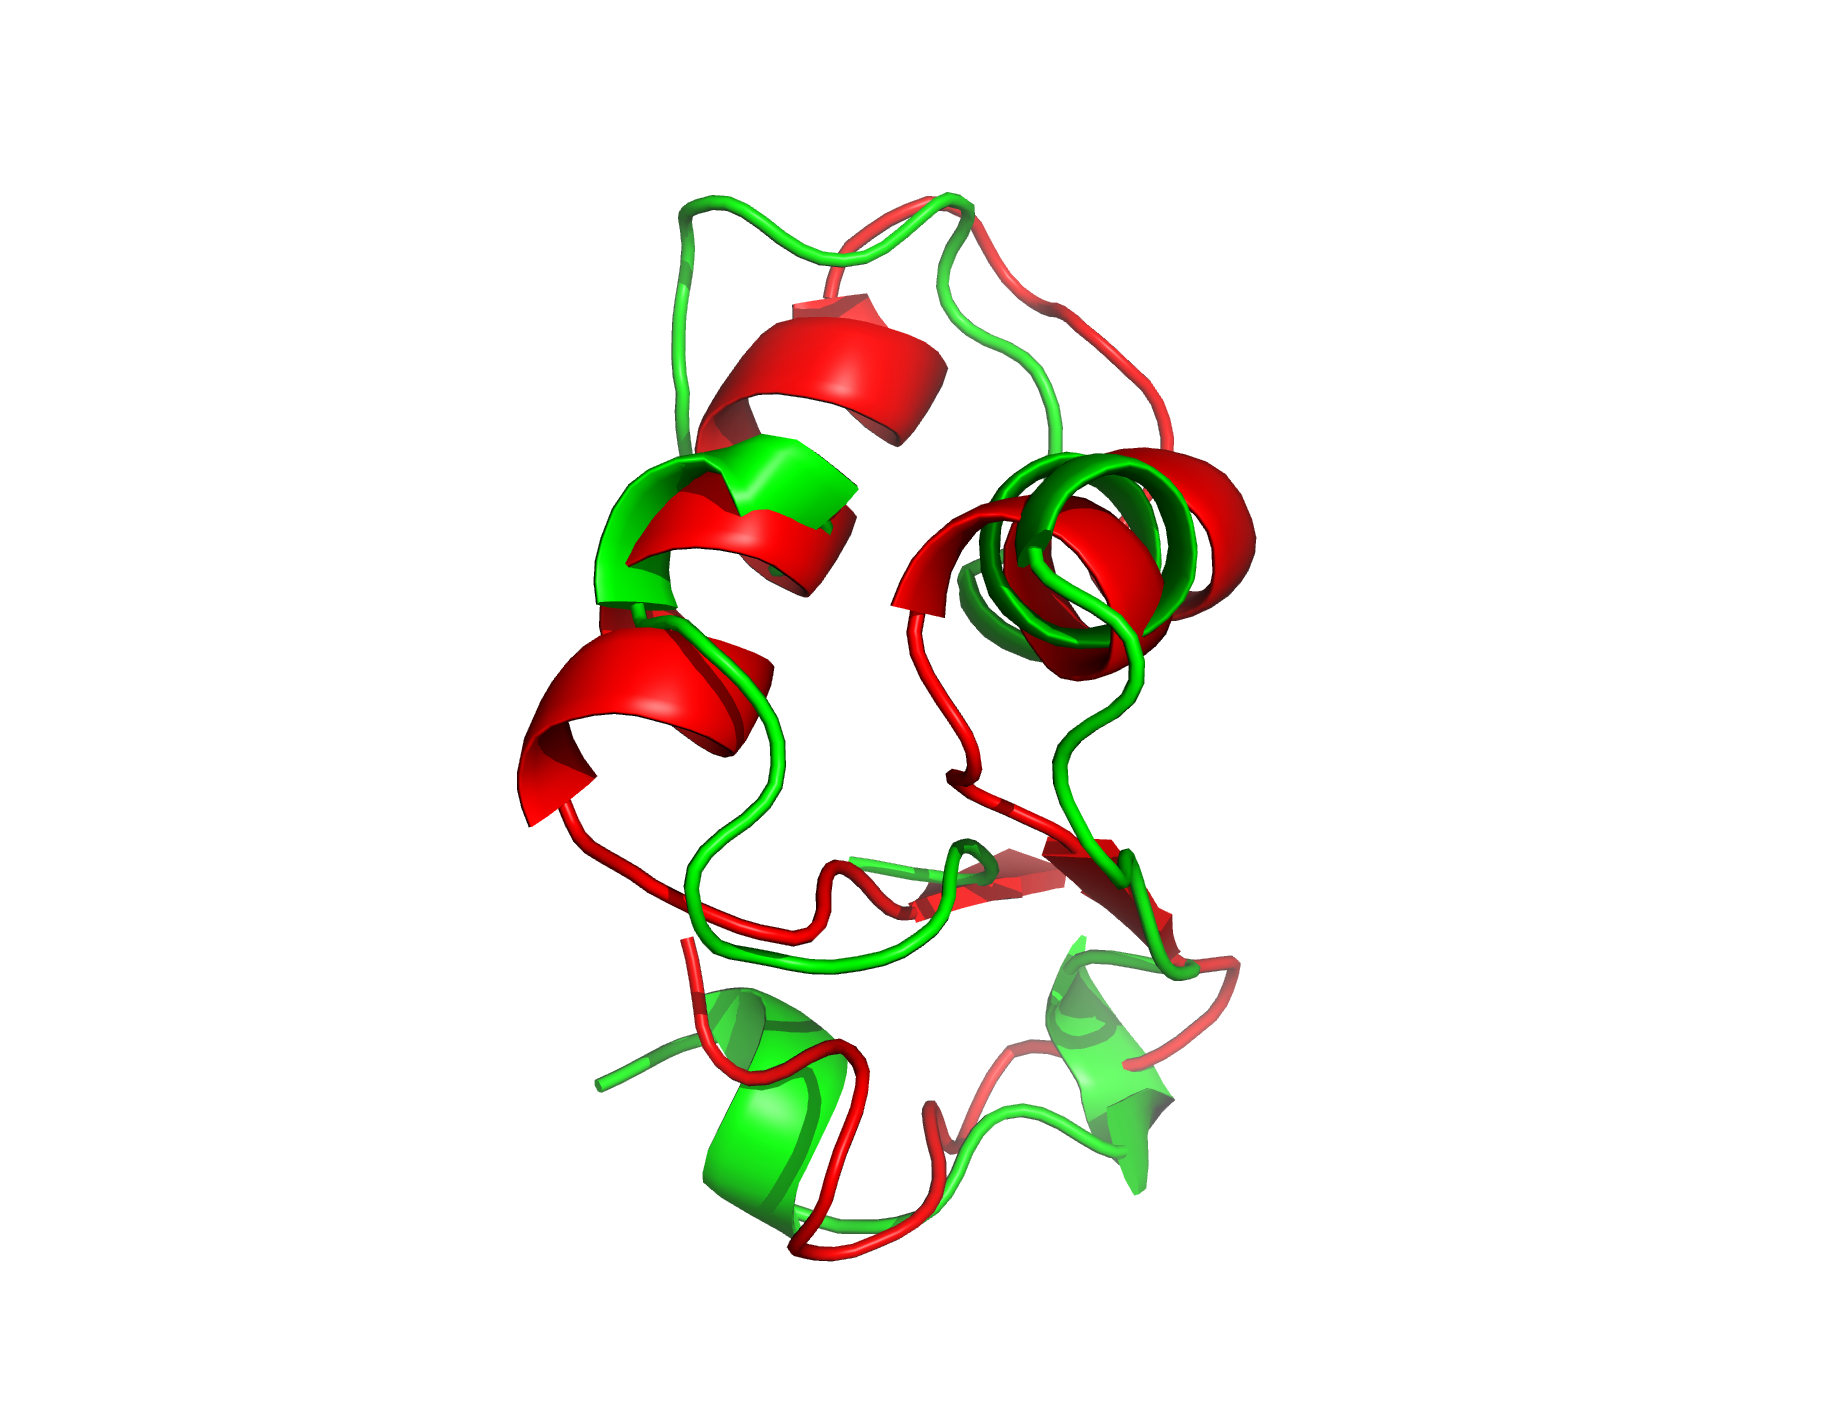
\includegraphics[width=0.9\linewidth]{Figuras/prots/1crn_render.png}
    \caption{Predicted Conformation of 1crn (green, light) over the Native Conformation}
    \label{fig:1crn-visual}
\end{figure}

\begin{figure}[ht]
    \centering
    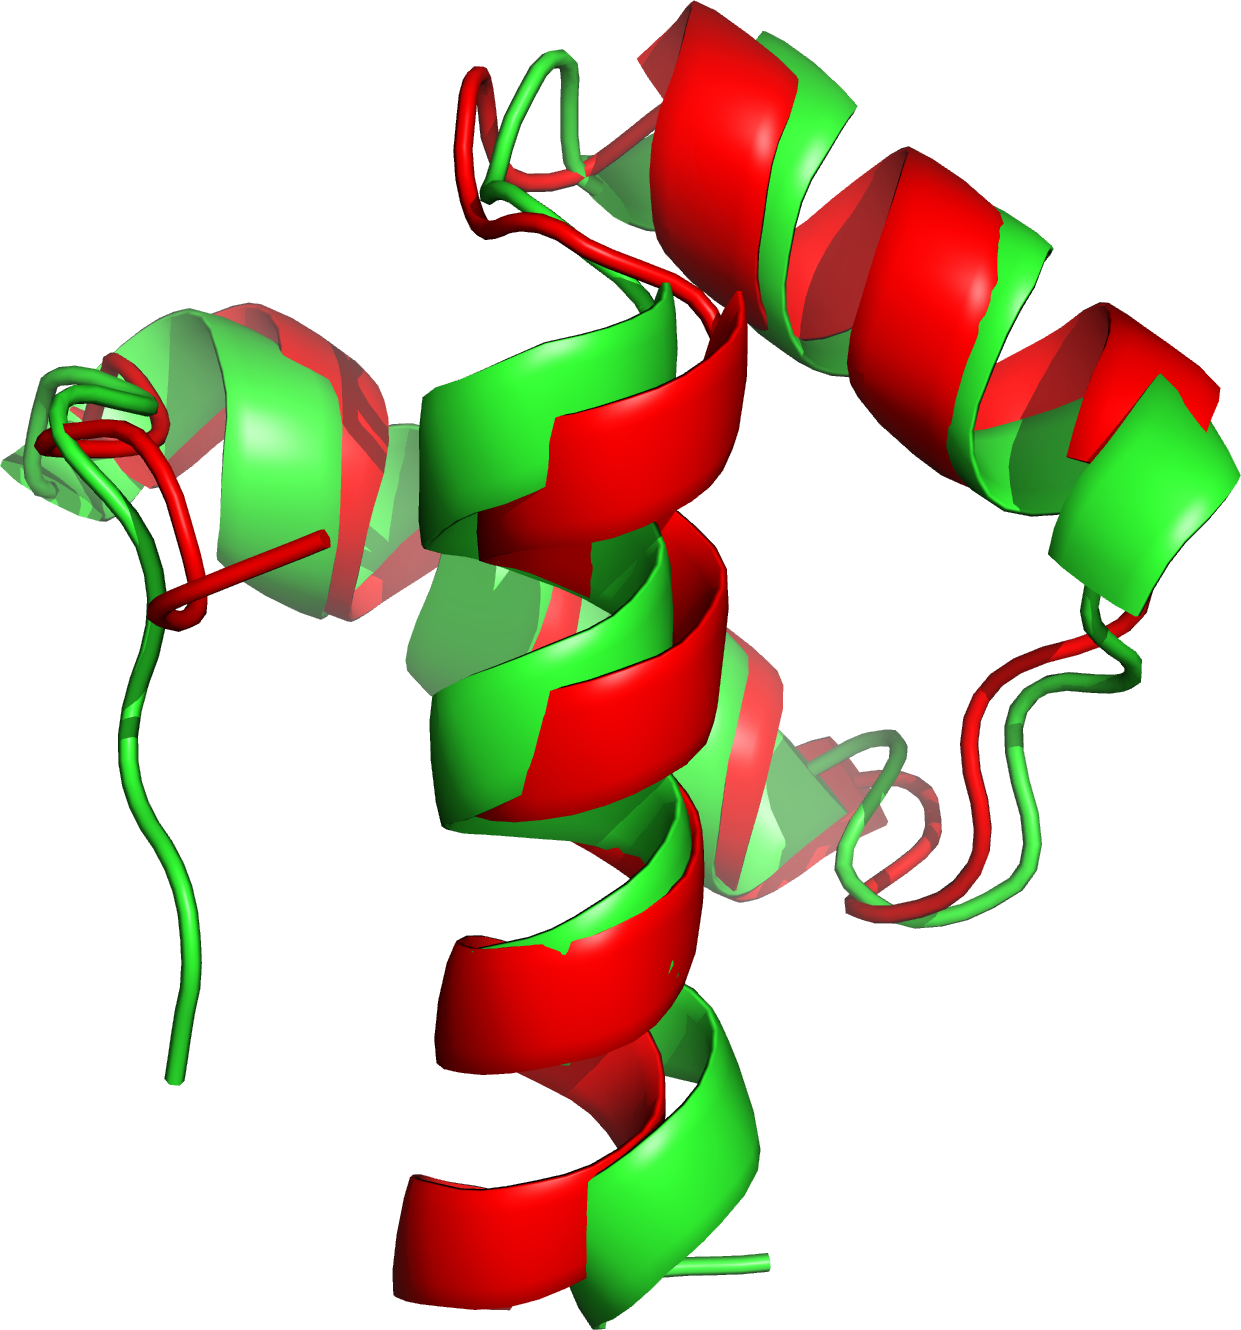
\includegraphics[width=0.9\linewidth]{Figuras/prots/1enh_render.png}
    \caption{Predicted Conformation of 1enh (green, light) over the Native Conformation}
    \label{fig:1enh-visual}
\end{figure}

\begin{figure}[ht]
    \centering
    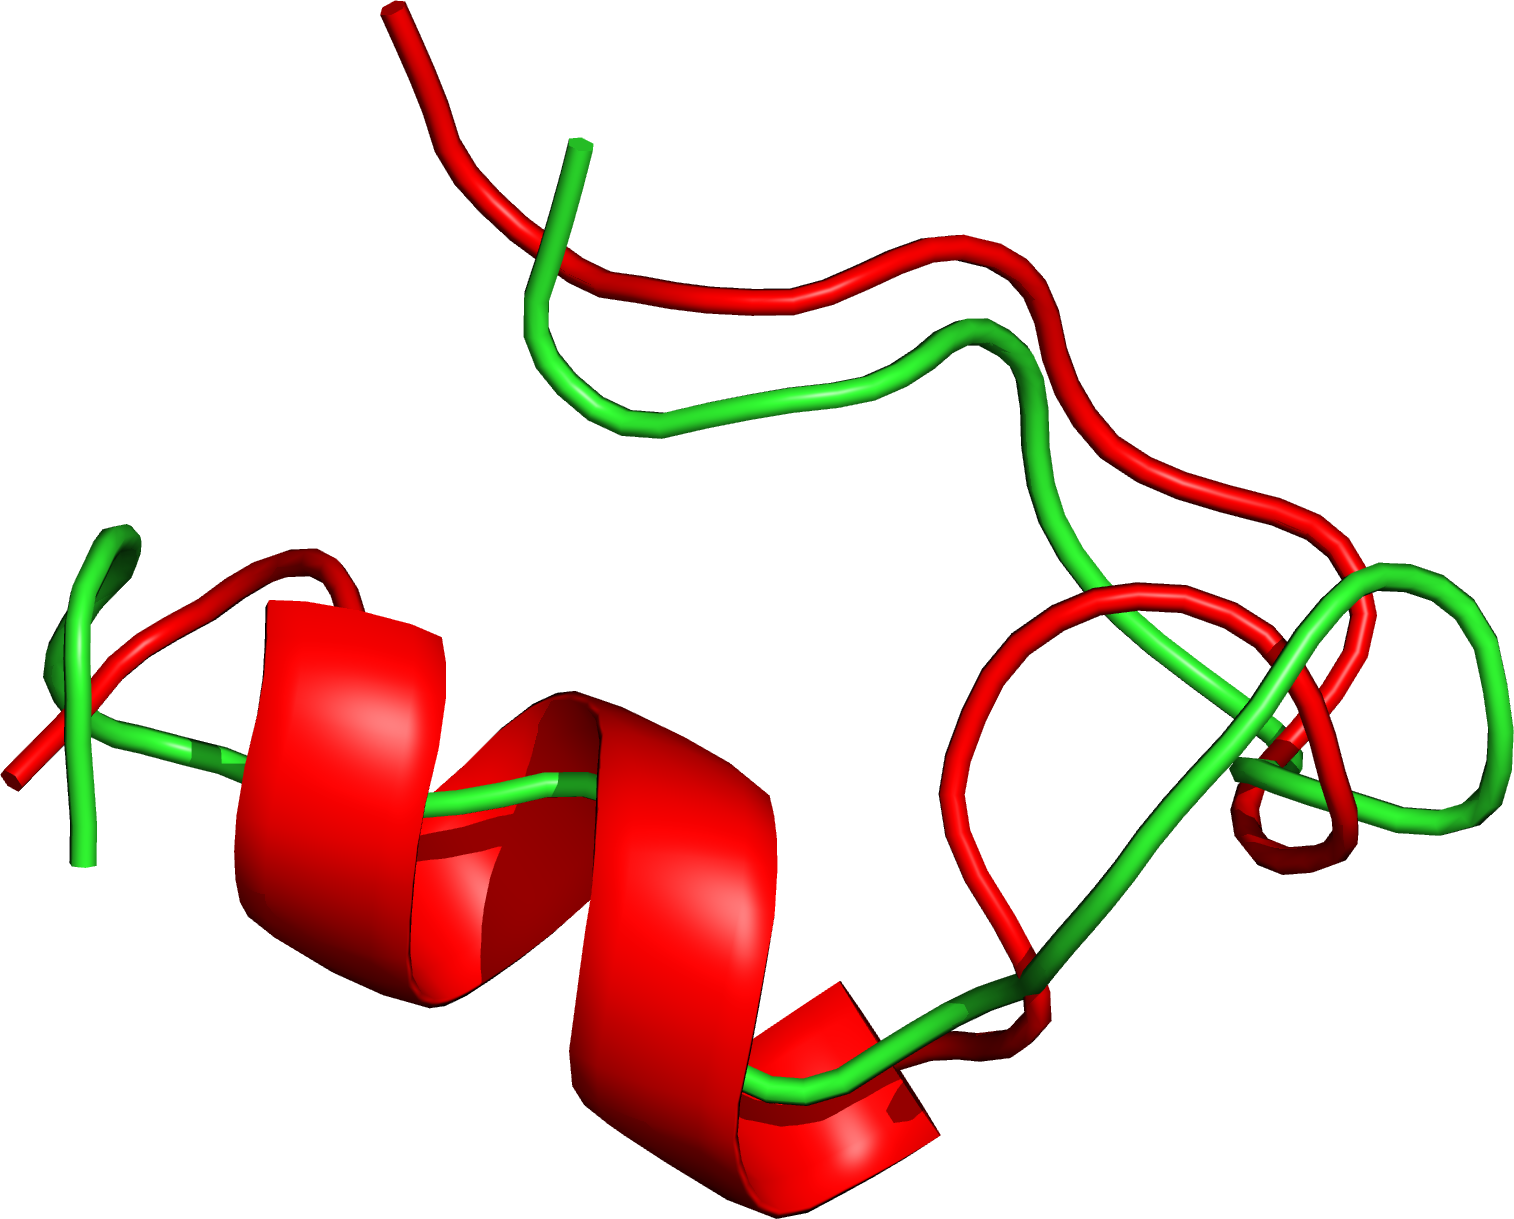
\includegraphics[width=0.9\linewidth]{Figuras/prots/1l2y_render.png}
    \caption{Predicted Conformation of 1l2y (green, light) over the Native Conformation}
    \label{fig:1l2y-visual}
\end{figure}

\begin{figure}[ht]
    \centering
    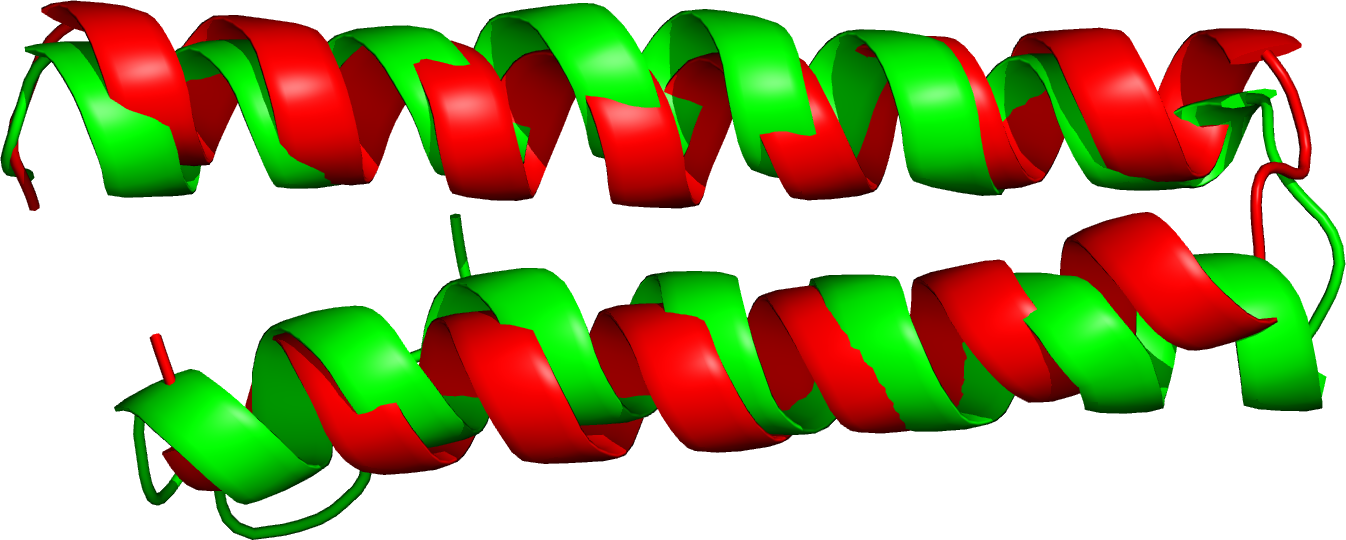
\includegraphics[width=0.9\linewidth]{Figuras/prots/1rop_render.png}
    \caption{Predicted Conformation of 1rop (green, light) over the Native Conformation}
    \label{fig:1rop-visual}
\end{figure}

\begin{figure}[ht]
    \centering
    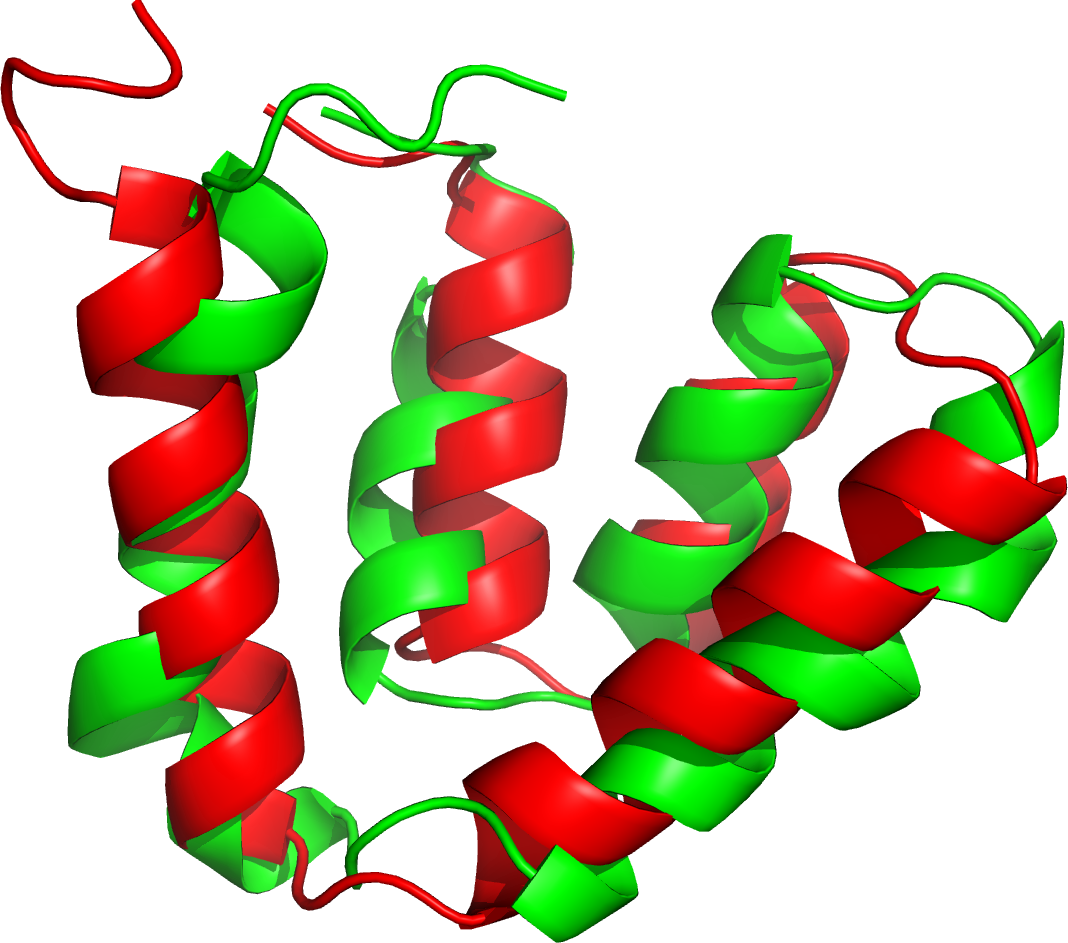
\includegraphics[width=0.9\linewidth]{Figuras/prots/1utg_render.png}
    \caption{Predicted Conformation of 1utg (green, light) over the Native Conformation}
    \label{fig:1utg-visual}
\end{figure}

\begin{figure}[ht]
    \centering
    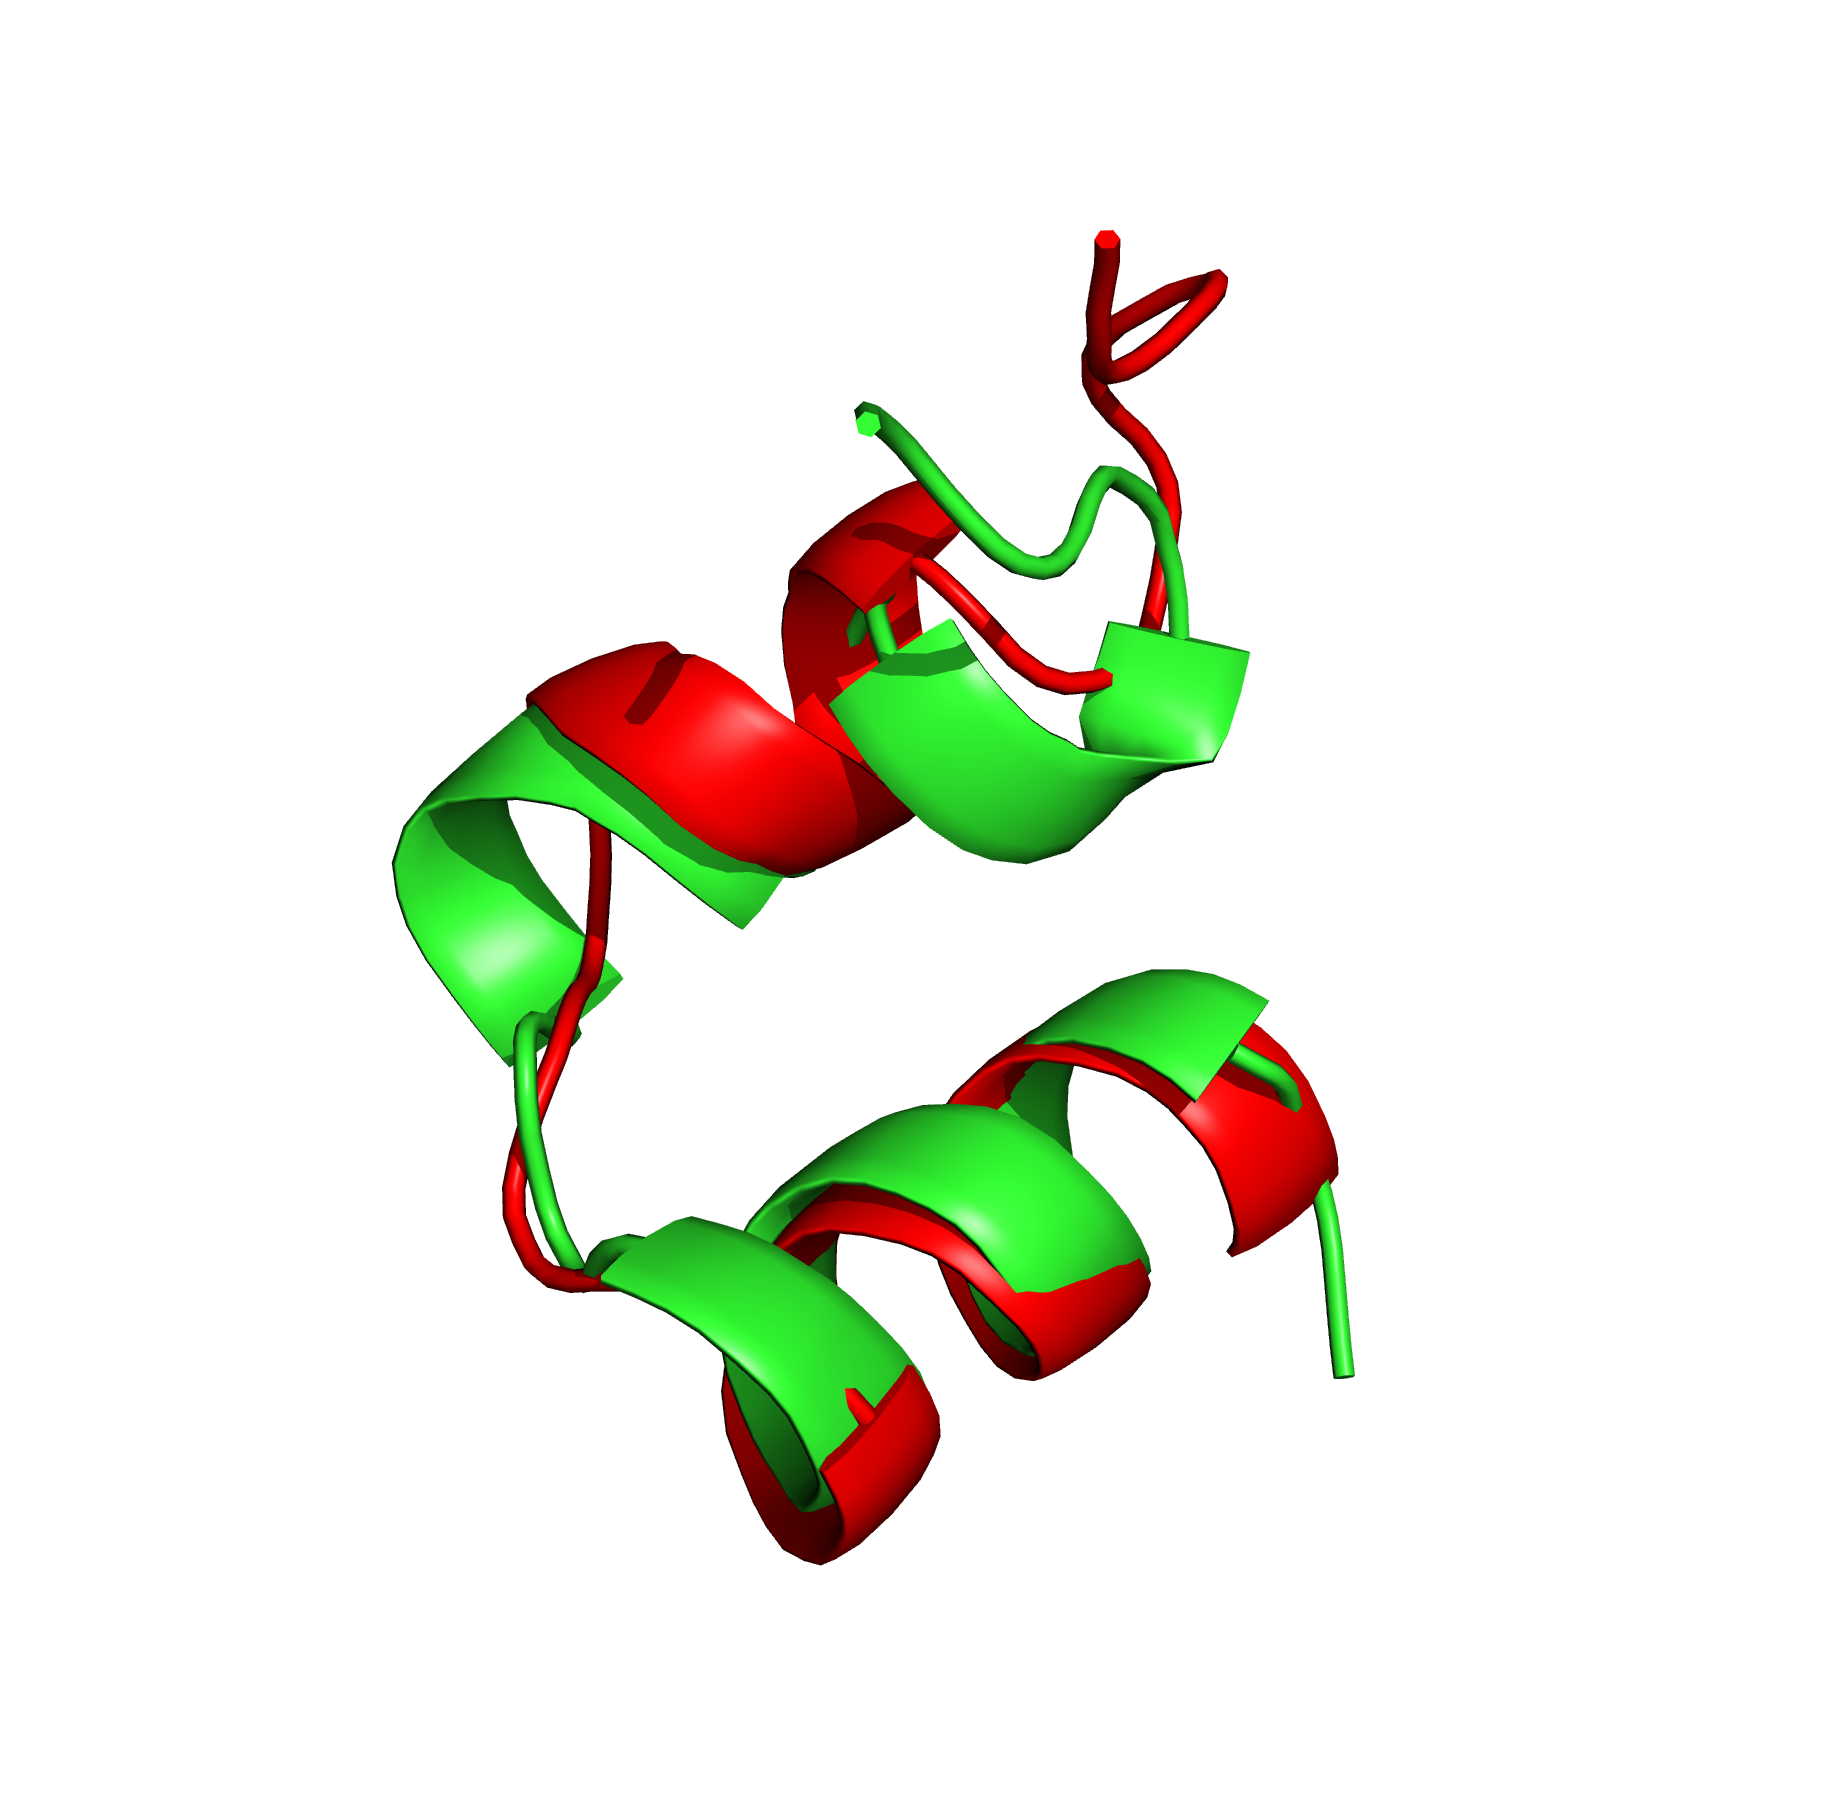
\includegraphics[width=0.9\linewidth]{Figuras/prots/1wqc_render.png}
    \caption{Predicted Conformation of 1wqc (green, light) over the Native Conformation}
    \label{fig:1wqc-visual}
\end{figure}

\begin{figure}[ht]
    \centering
    \includegraphics[width=0.9\linewidth]{Figuras/prots/1zdd_render.png}
    \caption{Predicted Conformation of 1zdd (green, light) over the Native Conformation}
    \label{fig:1zdd-visual}
\end{figure}

\begin{figure}[ht]
    \centering
    \includegraphics[width=0.9\linewidth]{Figuras/prots/2mr9_render.png}
    \caption{Predicted Conformation of 2mr9 (green, light) over the Native Conformation}
    \label{fig:2mr9-visual}
\end{figure}


\end{apendicesenv}

% \begin{anexosenv}
% 	\include{Partes/aneA}
% \end{anexosenv}

\end{document}
